\documentclass[12pt, a4paper]{report} \usepackage[titletoc]{appendix}
%\linespread{1.5}
%\usepackage{lineno}
%\linenumbers
\usepackage{amsmath}
\usepackage{float}
\usepackage[utf8]{inputenc}
\usepackage[T1]{fontenc}
\usepackage{lmodern}
\usepackage{microtype} % optional, for aesthetics
\usepackage{tabularx} % nice to have
\usepackage{booktabs}
\usepackage{makecell}
\usepackage{cite}
\usepackage{multirow}
\usepackage{hhline}
\usepackage{parskip}
\usepackage{wrapfig}
\usepackage{lscape}
\usepackage{xcolor}
\usepackage{ragged2e}
\usepackage{enumitem}
\usepackage{graphicx}
\usepackage{booktabs}
\setlist[enumerate]{label*=\arabic*.}
\usepackage{makecell}
\usepackage{kantlipsum}
\usepackage{enumitem}
\usepackage{tabularx}
\usepackage{appendix}
\usepackage{multirow}
\usepackage{hhline}
\usepackage{array}
\usepackage{subcaption}
%\usepackage{caption}
\graphicspath{{images/}} 
\usepackage{geometry}
\geometry{a4paper,left=4cm,top=3cm,bottom=3cm,right=3cm}
\usepackage{multirow}
\usepackage{hyperref}
\hypersetup{colorlinks=true,allcolors=blue}
\usepackage{hypcap}
\usepackage{courier}
\usepackage[linesnumbered,ruled]{algorithm2e}
\usepackage{listings}
\lstset{
    basicstyle=\ttfamily,
    frame=none, 
    breaklines=true,
    numbers=left,
    xleftmargin=2.5em,
    framexleftmargin=0em,
    emphstyle=\textbf,
    float=t
}
\lstdefinestyle{ocl}{
    emph={
        context, inv
    }
}
\lstdefinestyle{cbp}{
    basicstyle=\ttfamily\scriptsize,
    emph={
        session, create, type,
        set, to, add, hire
    }
}
\lstdefinestyle{xmi}{
    basicstyle=\ttfamily\scriptsize,
    emph={
        Node, children
    }
}
\lstdefinestyle{xml}{
    basicstyle=\ttfamily\scriptsize,
    emph={
        register, create, add, to, resource, at,
        from, eattribute, remove, ereference,
        set, unset, session, Roy, Jen,
        Moss, Richmond
    }
}
\lstdefinestyle{java}{
    basicstyle=\ttfamily\scriptsize,
    emph={
        case, $unset$,
        instanceof, else, if, void,
        new, UnsetEAttributeEvent,
        UnsetEReferenceEvent,
        @override, public, class, extends
    }
}
\lstdefinestyle{eol}{
    basicstyle=\ttfamily\scriptsize,
    emph={
        var, new, for, in, create, set, with, type, at,
        unset, to, add, remove, delete, register, move,
        from, position, from, move-within, session, \.
    }
}

\hyphenation{op-tical net-works semi-conduc-tor Hybrid-Change-Event-Adapter Hybrid-XMI-Change-Event-Adapater
    Hybrid-Neo-EMF-Change-Event-Adapater change-events Change-Event-Adapter EContent-Adapter notify-Changed Hybrid-Resource Resource-Impl state-Based-Resource cbp-Output-Stream Output-Stream Hybrid-Change-Event-Adapater Output-Stream Hybrid-XMI-Resource-Impl Hybrid-Neo-EMF-Resource-Impl Persistence-Resource change events
}


\definecolor{gray1}{gray}{0.90}
\definecolor{gray2}{gray}{0.95}

%\renewcommand{\thelstlisting}{\arabic{lstlisting}}
\renewcommand{\labelitemi}{$\bullet$}
\newcommand{\AndA}{\textnormal{\textbf{and }}}
\newcommand{\Is}{\textnormal{\textbf{is }}}
\newcommand{\Not}{\textnormal{\textbf{not }}}
\newcommand{\In}{\textnormal{\textbf{in }}}
\newcommand{\Or}{\textnormal{\textbf{or }}}
\newcommand{\eqnum}{\refstepcounter{equation}\textup{\tagform@{\theequation}}}

\begin{document}

\begin{titlepage}
\begin{center}

\textbf{\large Change-Based Model Persistence}

\vfill
\begin{figure}[ht]
\centering

\includegraphics[width=0.5\linewidth]{uoy}
\label{fig:uoy}
\end{figure}
\vfill

Alfa Ryano Yohannis\\
ary506@york.ac.uk

\vspace{1cm}

Supervisors:\\
Dimitris Kolovos\\
Fiona Polack\\
Horacio Hoyos Rodriguez
\vspace{1cm}

Department of Computer Science\\
University of York\\
United Kingdom\\
\vspace{1cm}
\today

\vfill
A Thesis Submitted in Partial Fulfillment of the Requirements\\
for the Degree of Doctor of Philosophy in Computer Science


\end{center}
\end{titlepage}


\begin{abstract}
\label{abstract}
\addcontentsline{toc}{chapter}{Abstract}
Most of the models in Model-Driven Engineering are persisted in state-based formats. While state-based persistence has certain advantages, it is problematic when it comes to detecting changes in large-scale models. As an alternative, this work proposes a change-based approach that involves persisting the full sequence of changes made to models. Persisting a model in a change-based format has the potential to deliver benefits over state-based persistence, such as the ability to detect changes, compare and merge models much faster and more precisely, which can then yield positive knock-on effects on helping developers compare and merge models in collaborative modelling environments. Nevertheless, change-based persistence also comes with downsides, such as ever-growing model file sizes and increased model loading time. So far, the initial implementation has been presented at the FlexMDE 2017 workshop, the proposed algorithm to optimise the loading time of change-based persistence has been presented at the ECMFA 2018 conference, and a paper discussing hybrid model persistence also has been presented at the Models and Evolution 2018 workshop. Currently, this research is still working on the change-based model comparison and merging. The thesis writing up is planned to start next year. An adjustment of the previous research plan is also presented in this report.
\end{abstract}

\tableofcontents
\addcontentsline{toc}{chapter}{Contents}

\cleardoublepage
\listoffigures
\addcontentsline{toc}{chapter}{List of Figures}

\cleardoublepage
\listoftables
\addcontentsline{toc}{chapter}{List of Tables}

\cleardoublepage
\lstlistoflistings
\addcontentsline{toc}{chapter}{Listings}

\cleardoublepage
\chapter*{Preface}

\cleardoublepage
\chapter*{Acknowledgements}
This work was partly supported through a scholarship managed by 
\emph{Lembaga Pengelola Dana Pendidikan Indonesia}
(Indonesia Endowment Fund for Education).

\cleardoublepage
\chapter*{Declaration}
I declare that this thesis is a presentation of original work and 
I am the sole author. This work has not previously been presented 
for an award at this, or any other, University. All sources are 
acknowledged as References.

\cleardoublepage
\chapter{Introduction}
\label{ch:introduction}
This Chapter briefly presents the background of this work as well as the research questions that will be addressed in this project. Several research objectives are then defined to answer the research questions. Lastly, research outputs and scoping are also presented. 

\section{Background}
\label{sec:background}
Most of the models in the context of Model-Driven Engineering are persisted in state-based formats. In such approaches, model files contain snapshots of the models' contents, and activities like version control and change detection are left to external systems such as file-based version-control systems and model differencing facilities. Activities such as change-detection (identifying parts that have changed in a model compared to a previous version) and model comparison (finding differences between models) are computationally consuming for state-based models \cite{Kolovos:2009:DMM:1564596.1564641}.  Thus, a new approach is needed to make the computation more efficient.

As an alternative to state-based persistence, this work proposes that a model can also be persisted in a change-based format, which persists the full sequence of \emph{changes} made to the model instead. The concept of change-based persistence is not new and has been used in persisting changes to software, object-oriented databases, and hierarchical documents \cite{DBLP:journals/entcs/RobbesL07,DBLP:conf/sde/LippeO92,DBLP:conf/caise/IgnatN05}. The change-based approach can improve detecting differences more precisely at the semantic level -- that is by providing finer-granularity information (e.g. types of changes, the order of the changes, elements that were changed, previous values, etc.) -- and therefore provide support to resolve them \cite{mens2002state}. The ordered nature of change-based persistence means that changes made to a model can be identified sequentially without having to explore and compare all elements of the model and its previous version. Based on these arguments, this work explores the advantages and shortcomings of change-based persistence as an alternative approach to state-based persistence for models conforming to 3-layer metamodelling architectures such as EMF and MOF. Persisting models in a change-based format can bring a number of envisioned benefits over state-based persistence, such as the ability to detect changes much faster and more precisely, which can then have positive knock-on effects on supporting (1) developers compare and merge models in collaborative modelling environments, and (2) incremental model management ( e.g. incremental query \cite{DBLP:conf/ecmdafa/RathHV12} and model-to-text transformation \cite{Ogunyomi2018}). 

Nevertheless, change-based persistence also comes with downsides, such as ever-growing model files \cite{DBLP:journals/entcs/RobbesL07,DBLP:conf/edoc/KoegelHLHD10} and increased model loading time \cite{mens2002state} which increase storage and computation costs. A model that is frequently modified will increase considerably in file size since every change is added to the file. The increased file size (proportional to the number of persisted changes) will, in turn, increase the loading time of the model since all changes have to be replayed to reconstruct the model's eventual state. These downsides have to be mitigated to enable the practical adoption of change-based persistence. One approach to reducing the file size of change-based models is by removing changes that do not affect the eventual state of the model. For the increased loading time, it can be mitigated by ignoring -- i.e. not replaying -- changes that are cancelled out by later changes or employing change-based and state-based persistence side-by-side so that the benefits of state-based persistence on loading time can be obtained. Other downsides are change-based persistence requires integration with existing tools -- since it is still a non-standard approach -- for its adoption \cite{koegel2010emfstore}, and still has limited support for standard, text-based version controls for collaborative development \cite{koegel2010emfstore}. These downsides can be addressed by developing a change-based persistence plugin for a specific development environment (e.g. Eclipse) and persisting changes in text-based format to support text-based version controls (e.g. Git, SVN).

\section{Research Questions}
\label{sec:research_questions}
The hypothesis of this work is that \textbf{``Change-based persistence reduces the execution time of model change-detection, model comparison, and model merging for large models compared to their execution time in state-based persistence, with acceptable trade-offs on loading and persisting time, memory footprint, and storage space consumption''}. The execution time is the time required to complete the processes (e.g. change-detection, model comparison, model merging, or persisting changes). Model change-detection is identifying changed elements of a model compared to its previous version/ancestor while the model comparison is finding the differences between two models that come from the same ancestor. Model merging is reconciling two models that come from the same ancestor and combining them to produce a new model. Using the term ``large models'' we refer to models with more than 1M elements, consistently with \cite{daniel2016neoemf,DBLP:conf/models/Espinazo-PaganCM11}. Model load time is the amount of time required to load a model into memory. Persisting changes is saving changes made to a model into a persistent representation (e.g. a file). Memory footprints are the sizes of memory used to execute the processes. Disk space consumption is the amount of storage consumed by the persistence. The term ``acceptable'' means the cost for memory extension is significantly lower than the cost for extending processor to reach the same execution time, and the loading and persisting time should be faster or slightly slower than the state-based approach.\\

To assess the validity of the hypothesis, this work aims to answer the following research questions: 
\begin{enumerate} 
    \item \textbf{How to persist models in a change-based format? How does it perform compared to state-based persistence on saving changes?} 
    
    The concept of change-based persistence has to be translated into an implementation in a modelling framework context so that it can be applied for model persistence, and therefore its impact on model change-detection, model comparison, and model merging can be assessed.
    %It is expected that every change made to a model can be persisted by the implementation. Replaying all the persisted changes can reconstruct the same model as the model persisted in state-based format. 
    %It is also expected that change-based persistence will outperform state-based persistence on time required for saving changes since change-based persistence will only require persisting changes of a model while state-based persistence will persist the whole model. 
    
    %\item \textbf{How to mitigate the ever-growing file size and increased loading time of change-based models? To what extent can they be reduced?} 
    %
    %Change-based persistence comes with the downsides of larger file sizes and increased loading time. Mitigating these side effects will is essential for facilitating the practical adoption of change-based persistence. For the increased file size, the size can be reduced by removing changes that do not affect the eventual state of the model. For the increased loading time, it can be mitigated by ignoring -- not replaying -- changes that are cancelled out by subsequent changes or employing change-based and state-based persistence side-by-side (hybrid approach). Employing both persistence side-by-side can maintain the benefit of state-based persistence on loading time. It is expected that the mitigation approaches will (1) lead to loading time that is closer to the loading time of state-based format, (2) significantly load models faster than loading change-based models naively, and (3) significantly reduce change-based model file sizes compared to the naive approach on saving change-based model files. 
    %
    %For reducing the loading time using change-based and state-based persistence side-by-side, the impact of the approach will also be investigated on several qualities. It is expected that a hybrid persistence approach will: (1) be significantly slower than change-based persistence on persisting changes and slightly slower than state-based persistence on saving time as the hybrid approach will need to save changes to the other two types of persistence, (2) consume more disk space compared to change-based or state-based persistence since the hybrid approach will use them both simultaneously, and (3) facilitate loading time that is closer to the loading time of state-based persistence. 
    
    \item \textbf{How to detect changes in change-based models -- comparing them to their ancestors/previous versions? To what extent does change-detection in change-based models perform compared to change-detection in state-based models?} 
    
    The purpose of using change-based persistence in this work is to improve change-detection. The change-based persistence will have change-detection time that is smaller than the change-detection time of state-based persistence.        
    
    \item \textbf{How to compare change-based models that come from the same ancestor? How does the comparison of change-based models perform compared to the state-based model comparison?} 
    
    The knock-on effect of faster change-detection on model comparison will also be investigated. Due to the nature of change-based models, the mechanism to perform change-based model comparison will differ substantially from the current state-based model comparison. It is expected that comparison of change-based models will be significantly faster than the comparison of state-based models.
    
    \item \textbf{How to merge different change-based models that come from the same ancestor? How does the merging perform compared to model merging in state-based persistence?}
    
    Another knock-on effect of faster change-detection of change-based persistence is faster model merging. Similar to the change-based model comparison, the mechanism to merge change-based models will differ substantially from merging state-based models. It is expected that the change-based model merging will be much faster than state-based model merging.   
    
\end{enumerate}

\section{Research Objectives}
\label{sec:research_objectives}
This research aims to meet the following research objectives to answer the research questions.
\begin{enumerate}
    \item Develop an implementation of change-based persistence so it can be applied to persist models in change-based format, and evaluate the correctness of change-based models that it produces and its performance on saving changes against state-based persistence. 
    \item Develop a solution to detect changes in change-based models, and compare its execution time and memory footprint against change-detection in state-based models.
    \item Develop a solution to compare change-based models, and compare its execution time and memory footprint against model comparison in state-based models.
    \item Develop a solution to merge different change-based models, and compare its execution time and memory footprint against model-merging in state-based models. 
\end{enumerate}

\section{Research Outputs}
\label{sec:research_outputs}
By the end of this research, these following outputs will have been produced:
\begin{enumerate}
    \item Prototypes for change-based persistence. 
    \item Solutions -- including their implementation and evaluation -- for file size and loading time reduction, change-detection (finding parts that already changed of a model compared to its previous version/ancestor), model comparison (finding differences between models that come from the same ancestor), and model merging of change-based persistence.
    \item Publications and a thesis documenting the outcomes of this research.
\end{enumerate}


\section{Research Scope}
\label{sec:research_scope}
The scope of this research will be restricted to models conforming to 3-level metamodelling architectures. The Eclipse Modelling Framework will be used, as a representative example of such architectures, for the implementation of all algorithms and prototypes.

\chapter{Thesis Structure}
\label{sec:Thesis Structure}
This section provides the description of the planned thesis structure and its progress. Each subsection corresponds to a chapter in the thesis report and describes the purpose, contents, and progress of the chapter. Some of the contents have been discussed in this research's Progress Report \cite{yohannis2017progress}, Thesis Outline \cite{yohannis2018outline}, and written papers \cite{DBLP:conf/models/YohannisKP17,yohannis2018towards,DBLP:conf/models/YohannisRPK18}, and they will be transferred to the thesis report with proper adjustments. The planned time frame for each chapter is presented in Chapter \ref{ch:plan}.

\section{Chapter 1: Introduction}
\label{sec:chapter_1_introduction_plan}
This chapter is intended to present the motivation and purpose of this research. It will comprise the (1) background of the research as well as the (2) research hypothesis, (3) research questions, (4) research objectives, (5) research outputs, and (6) research scope. All of these contents have been defined in the Progress Report \cite{yohannis2017progress} and  this Thesis Audit, and they will be transferred to the Thesis Report with proper adjustments. 

\section{Chapter 2: Literature Review}
\label{sec:chapter_2_literature_review_plan}
This chapter is dedicated to summarise work related to change-based persistence and comparison, critically assesses the advantages and disadvantages of current approaches, and seek the opportunities to contribute novel knowledge to the field. The chapter will comprise (1) change-based approaches in software engineering, (2) change-based model persistence, (3) state-based model persistence, (4) text-based comparison and merging, (5) state-based model comparison and merging, and (6) change-based model comparison and merging. Most of these topics have been discussed briefly in the Progress Report \cite{yohannis2017progress}. %However, text-based comparison, state-based model comparison, and change-based model comparison and merging need more literature review and deeper analysis to support defining a new approach for change-based model comparison and merging.

\section{Chapter 3: Change-based Model Persistence}
\label{sec:chapter_3_Change-based_model_ersistence_plan}
This chapter is planned to present the concept of change-based model persistence and its core implementation. The chapter will comprise the concept of change-based model persistence, and the design of the core implementation. The implementation is evaluated by comparing the eventual model produced by replaying a change-based representation to the same model but loaded from a state-based persistence (e.g. XMI). These contents have been published in a workshop \cite{DBLP:conf/models/YohannisKP17}.


\section{Chapter 4: Optimised Loading of Change-based Models}
\label{sec:chapter_4_optimised_loading_change_based_model_persistence}

Change-based persistence comes with a downside of ever-growing file sizes \cite{DBLP:journals/entcs/RobbesL07,DBLP:conf/edoc/KoegelHLHD10} which causes increased loading time \cite{mens2002state}. Reducing the loading time is essential to facilitate the practical adoption of change-based persistence. One way to reduce the increased loading time is by ignoring -- not replaying -- changes that are cancelled out by subsequent changes. 

To evaluate the efficiency of the proposed approach, the optimised loading is compared to a naive loading of a change-based representation and loading the same model from a state-based representation. They are compared on time required to load models and the memory footprint after loading models. Evaluation is also performed on time required for persisting changes between change-based and state-based persistence to show the benefit of change-based persistence on saving changes. 

This chapter is intended to present the optimisation approach along with its implementation and evaluation. The contents of this chapter will be largely based on an accepted conference paper \cite{yohannis2018towards}. 


\section{Chapter 5: Hybrid Model Persistence}
\label{sec:chapter_5_hybrid_model_persistence}
While optimised loading is faster than the naive loading, the benefits are moderate and that the optimised loading is still slower than loading from a state-based representation \cite{yohannis2018towards}. This finding has motivated the design and development of a hybrid persistence approach, that is augmenting a change-based representation with a state-based representation. 

The hybrid model persistence approach is evaluated by comparing it to state-based persistence (e.g. XMI, NeoEMF \cite{daniel2016neoemf}) on time, memory footprint, and storage space required for loading models and persisting changes. The evaluation is also performed on time required for detecting changes between hybrid and state-based persistence to show the benefit of change-based persistence over state-based model comparison. 

This chapter is dedicated to present the hybrid model persistence approach together with its implementation and evaluation. The contents of this chapter will be largely based on a workshop paper \cite{DBLP:conf/models/YohannisRPK18} that is currently under review. 

\section{Chapter 6: Change-based Model Comparison}
\label{sec:chapter_6_change_based_model_comparison}
This chapter will present a change-based model comparison algorithm with its implementation and evaluation. Change-based persistence is expected to speed-up model comparison because the information required to identify changes is already contained in the models' representation. 

The proposed algorithm will be evaluated by comparing it to state-based model comparison (e.g. EMF Compare \cite{eclipse2017compare}) on the time and memory footprint required to find all differences between models. This research will derive synthetic models from branches of real-world software projects as datasets in the evaluation. The alternative strategy is to perform an experiment on modellers. They will be asked to develop models in parallel. The produced models will be upscaled and used in the evaluation. 

The findings of this chapter will be published together with the findings of Chapter 7.


\section{Chapter 7: Change-based Model Merging}
\label{sec:chapter_7_change_based_model_Merging}
This chapter is planned to present change-based model merging. After identifying the differences between two versions of a change-based model, there is a need to reconcile all the differences into a new version of the model. Thus, conflicts between the two versions have to be identified and resolved -- using predefined rules or based on users' decisions, and by then merging steps can be determined to merge the two versions. 

Similar to change-based model comparison in Section \ref{sec:chapter_6_change_based_model_comparison}, the proposed merging approach will also be evaluated by comparing it to the merging of state-based persistence (e.g. EMF Compare) on the affected time and memory footprint. The evaluation will also use the same datasets in Section \ref{sec:chapter_6_change_based_model_comparison}.

The findings of this chapter will be published together with the findings of Chapter 6.
\chapter{Literature Review}
\label{ch:literature_review}

This chapter presents the literature review of this study. Firstly, it discusses some work on model persistence by highlighting some key characteristics -- unique features, strong points, and downsides -- of some existing implementations. It then summarises the advantages and drawbacks of the two main types of persistence: state-based and change-based persistence, and introduces desirable characteristics for a new change-based persistence implementation. This chapter then reviews the related work on identifying differences and detecting conflicts between versions of models. It then presents the current challenges that model differencing and conflict detection are dealing with as well as the downsides of existing approaches in tackling the problems, which gives motivation to this research to come up with a new solution. Lastly, the conclusions of the literature review are presented.  

%\section{Introduction}
%\label{sec:introduction_2}
%The research introduced in this thesis aims at enabling high-performance model differencing and conflict detection through change-based persistence. This goal can only be delivered if this study can identify the strong points and downsides of current approaches of model persistence, differencing, and conflict detection and incorporate and address them in the solution of this research. Knowing the strong points and downsides is also helpful to find rooms for improvement and to deliver novelties in the solution. A literature review needs to be conducted in order to identify the strong points and downsides. The literature review of this study is presented in this chapter.
%
%Once the strong points, downsides, rooms for improvements and novelties have been gathered, they all need to be elaborated into a design of a solution. The solution needs to be translated into a working implementation, experimented, and evaluated to answer the research questions of this study. This sequence of work has to be guided by a research method to ensure it has been carried out properly. The research method employed in this study is also presented in this chapter. 
%
%The rest of this chapter is structured as follows. Section \ref{sec:model_persistence} reviews some key implementations of model persistence; their strong points and drawbacks. Section \ref{sec:model_differencing_and_conflict_detection} presents the current approaches in model differencing and conflict detection, their existing challenges, as well as the motivation for a new change-based model persistence. Section \ref{sec:benefits_and_novel_capabilities} presents briefly the research method employed in this research. Section \ref{sec:conclusions_2} concludes this chapter.

\section{Models in This Research}
\label{sec:models_in_this_research)}

A model is an abstract representation of an entity \cite{volter2013model}. It can be used for different purposes: as a sketch to communicate a system, as a blueprint to define the specification of a system, or as a modifiable artefact to generate a working system \cite{fowler2019umlmode}. In model-based software engineering, the latter is the scenario in which models are mainly used. 
In the scenario, a model is created using a modelling language, and the model should conform to its metamodel -- an abstraction that describes the model. Later, the model can be transformed to generate a software artefact through model transformation/code generation \cite{brambilla2012model}. The software artefact, its model, and the model's metamodel create a 3-layered abstraction which is known as the 3-layer metamodelling architecture.  

Eclipse Modeling Framework (EMF) \cite{steinberg2008emf} is a technical implementation of such architecture. It is a framework and code generation facility that allows developers to define metamodels, create models, and to generate implementations of the models \cite{steinberg2008emf}. In this research and literature review, we focus on models and modelling tools that support the 3-layer metamodelling architecture of EMF.

\section{Model Persistence}
\label{sec:model_persistence}
In constructing models, modelling tools should be able to support model persistence so that models that are under construction can be saved at any time and reloaded for further modification. Majority of the tools persist models in a state-based format that is capturing a snapshot of a model at a time and then persist its entire state into storage. The model state can be persisted in different forms, such as text files, relational databases, or NoSQL databases.

\subsection{Text Files}
\label{sec:text_file}
The simplest and most common way to save a model is to persist it into a text file. By default, modelling tools that support the 3-layer metamodelling architectures of Eclipse Modeling Framework (EMF) \cite{steinberg2008emf} persist a model in a text file with a format of Metadata Interchange (XMI) -- a standard issued by Object Management Group (OMG) for exchanging metadata information via Extensible Markup Language (XML) \cite{omg2018xmi}. 

Since it is the default standard for persisting EMF models, it is supported by  most modelling tools. In order to modify a model persisted in an XMI file, such as performing create, read, update, delete (CRUD) operations, a tool has to de-serialise and load the model from the file into memory. This can be a problem when we only want to make a small number of changes but the size of the model is very large -- it takes considerable time and memory to load the model. Also, when saving, the model has to be persisted in its entirety causing inefficiency when we only made small number of changes. Since it is a text-based file, the model can be duplicated and shared with minimum effort, e.g. through manual copy or version control systems (e.g. Git \cite{git2019about}, SVN \cite{apache2019svn}). However, for model differencing (see Section \ref{sec:model_differencing_and_conflict_detection}), text-based differencing \cite{DBLP:journals/algorithmica/Meyers86} cannot be applied accurately to XMI files since essentially they are tree documents which require different differencing approaches \cite{wang2003xdiff}.

\subsection{Relational Databases}
\label{sec:relational_databases}
Models can also be persisted into relational databases. EMF Teneo \cite{eclipse2017teneo} is a solution that integerates EMF with existing persistency solutions, such as Hiberbate \cite{hibernate2019hibernateorm} and EclipseLink \cite{eclipse2019eclipselink}. Thus it can persists EMF models into relational database backends. In this way, EMF Teneo can utilise the power of storage, caching, and querying of the database backends. It also supports the automatic mapping of models to relational model schema with flexible mapping customisation. Using relational databases as its backends enables EMF Teneo to support lazy loading of models. So, when performing CRUD operations, it only loads and saves relevant elements and features -- not the entire model -- into and from memory, which is efficient in terms of memory usage.

Similar to EMF Teneo, Connected Data Objects (CDO) \cite{eclipse2019cdo} also supports persisting models into various database-backends model persistence (e.g. relational and NoSQL databases). It is a development-time model and metamodel repository as well as a distribution and runtime persistence framework for EMF-based application systems. It supports model versioning and can perform model differencing and conflict detection -- it uses EMF Compare \cite{emfcompare2018developer} to perform the comparison \cite{cdo2019emfcompare}. One downside of CDO is its adoption necessitates the use of a separate version control system (e.g. a Git repository for code and a CDO repository for models), which introduces fragmentation and administration challenges \cite{barmpis2014evaluation}.

\subsection{NoSQL Databases}
\label{sec:NoSQL Databases}
In the era where data is abundant and models are getting larger in sizes, the ability to handle large models is necessary. Tools, such as Morsa \cite{DBLP:conf/models/Espinazo-PaganCM11} and NeoEMF \cite{daniel2016neoemf}, has been developed to persist models into non-relational (NoSQL) databases. Morsa saves models in documents with MongoDB as its backend \cite{mongodb}, while NeoEMF persists models in multi, NoSQL backends: Neo4j \cite{neo4j2019neo4j} for Graph, MapDB \cite{mapdb2019mapdb} for Map, and Apache HBase \cite{apache2019hbase} for Column datastores. The advantages of using NoSQL databases are that users are given options to choose which datastores -- wih some degree for configuration -- that best fit with the characteristics of their models and metamodels and to maximise the features  the backends provide, such as lazy loading, caching, etc. Neither Morsa nor NeoEMF provide built-in support for versioning and models are eventually stored in binary files/folders which are known to be a poor fit for text-oriented version control systems like Git and SVN. 

\subsection{Change-based Representation}
\label{sec:change_based_representation}
All the solutions previously mentioned persist models in state-based format. EMF Store \cite{koegel2010emfstore} takes a different approach; it persists models in a change-based representation. EMF Store appears to be the only current implementation of change-based persistence for EMF models.

EMF Store is a model repository and supports collaborative editing and versioning of models \cite{emfstore2019what}. Instead of using standard text-oriented version controls (e.g., Git, SVN) for model versioning, EMF Store has its own dedicated, change-based, model-oriented versioning mechanism. Models are shared through a server and distributed to client applications. Clients can modify the models in parallel, offline or online, and synchronize with the server. Conflicts caused by concurrent modification are detected automatically and can be resolved interactively by users. The historical changes of models are kept on the server, and different versions of a model as well as changes that produce the them can be retrieved from the server. 

In EMF Store, to version models, a project has to be created first. A project can contain one or more models. Every project has a version history, and each version represents a commit of a client. A commit sends a package of changes to the server. The package itself contains a collection of operations applied to a version that transforms it to a newer version or can be said as the deltas between the two versions. The operations can be add, delete, set, unset or move that modifies an element or feature, or they can be a composite operation, an operation that consists of many operations, e.g. refactoring that moves a method to a superclass.

To obtain a specific version of an existing project, a client can perform a checkout. This version is called the base version on the client side. The client then can perform modification to this version. Every operation applied to the version is recorded by EMF Store. When the client commits, these operations are put into one package and sent to the server. If the base version is still the head version of the project on the server, the commit is accepted, and a new version is created. If they are different, it means that there is another client that already committed its changes to the server. Thus the current client has to synchronise it by updating its local project. This is the state where conflicts can happen potentially between the incoming and local changes, that is when they modify the same element or feature of a model. EMF Store performs conflict detection to identify conflicts automatically. The mechanism of EMF Store to identify conflicts is discussed in detail in Section \ref{sec:emfstore_conflict_detection}.

\begin{table*}[]
  \centering
  \caption{Advantages and downsides of different model persistence solutions.}
  \label{table:model_persistence_comparison}
\begin{scriptsize}
  \begin{tabular}{
      |>{\centering\arraybackslash}m{0.1\linewidth}
      |>{\centering\arraybackslash}m{0.4\linewidth}
      |>{\centering\arraybackslash}m{0.4\linewidth}
      |}
    \hline
    \textbf{Products} & \textbf{Advantages} & \textbf{Downsides} \\
    \hline
    XMI 
    &
    \begin{minipage}[t]{\linewidth}
      \raggedright
      \begin{itemize}[leftmargin=7pt]
        \setlength
        \item[+] default standard, widely supported
        \item[+] easy to be duplicated and shared by manual copy or text-oriented version controls
      \end{itemize}
    \end{minipage}
    & 
    \begin{minipage}[t]{\linewidth}
      \raggedright
      \begin{itemize}[leftmargin=5pt]
        \setlength
        \item[--] requires loading the entire model to modify
        \item[--] a model is saved in its entirety
        \item[--] supports text-oriented version controls, but applying text-based differencing might produce inaccurate results    
      \end{itemize}
    \end{minipage}
    \\
    \hline
    Teneo 
    & 
    \begin{minipage}[t]{\linewidth}
      \raggedright
      \begin{itemize}[leftmargin=7pt]
        \setlength
        \item[+] supports lazy loading, only load and save affected elements and features when performing CRUD operations
        \item[+] has the capabilities supported by database backends: rollback, caching, etc. 
      \end{itemize}
    \end{minipage}
    &
    \begin{minipage}[t]{\linewidth}
      \raggedright
      \begin{itemize}[leftmargin=7pt]
        \setlength
        \item[--] does not support model versioning, comparison, and merging
        \item[--] multiple concurrent accesses can cause a bottleneck
%        \item[--] performance on loading and saving for CRUD operations depends on the database backend
        \item[--] poor fit for text-oriented version controls since models are persisted in database
      \end{itemize}
    \end{minipage} 
    \\
    \hline
    CDO
    &
    \begin{minipage}[t]{\linewidth}
      \raggedright
      \begin{itemize}[leftmargin=7pt]
        \setlength
        \item[+] supports lazy loading, only load and save affected elements and features when performing CRUD operations
        \item[+] supports model versioning, comparison, and merging
        \item[+] has the capabilities supported by database backends: rollback, caching, etc. 
      \end{itemize}
    \end{minipage}
    &
    \begin{minipage}[t]{\linewidth}
      \raggedright
      \begin{itemize}[leftmargin=7pt]
        \setlength
%        \item[--] performance on loading and saving for CRUD operations depends on the database backends
        \item[--] fragmentation and administration challenges due to separation of version controls between models and code
        \item[--] poor fit for text-oriented version controls since models are persisted in database
      \end{itemize}
    \end{minipage} 
    \\
    \hline
    Morsa \& NeoEMF 
    & 
    \begin{minipage}[t]{\linewidth}
      \raggedright
      \begin{itemize}[leftmargin=7pt]
        \setlength
        \item[+] supports lazy loading, only load and save affected elements and features when performing CRUD operations
        \item[+] has the capabilities supported by NoSQL backends: handling big data, graph data, etc.
      \end{itemize}
    \end{minipage}
    &
    \begin{minipage}[t]{\linewidth}
      \raggedright
      \begin{itemize}[leftmargin=7pt]
        \setlength
        \item[--] does not support model versioning, comparison, and merging
%        \item[--] performance on loading and saving for CRUD operations depends on the database backends
        \item[--] poor fit for text-oriented version controls since models are persisted in database
      \end{itemize}
    \end{minipage} 
    \\
    \hline
    EMF Store
    &
    \begin{minipage}[t]{\linewidth}
      \raggedright
      \begin{itemize}[leftmargin=7pt]
        \setlength
        \item[+] supports semantic versioning of models that allows model merging and conflict detection to be more effective
      \end{itemize}
    \end{minipage}
    &
    \begin{minipage}[t]{\linewidth}
      \raggedright
      \begin{itemize}[leftmargin=7pt]
        \setlength
        \item[--] requires loading the entire model to modify
        \item[--] a model is saved in its entirety even for small changes
        \item[--] persists models in the forms of files/folders and using its own mechanism for model versioning thus poor fit for text-oriented version controls
      \end{itemize}
    \end{minipage} 
    \\
    \hline
  \end{tabular}
\end{scriptsize}
\end{table*}
  
The primary motivation EMF Store applies change-based approach is that calculating the differences between two versions in state-based persistence can be expensive and less accurate \cite{emfstore2019versioning} (state-based model differencing identify differences using LCS algorithms \cite{emfcompare2018developer,DBLP:journals/algorithmica/Meyers86}, not from the real changes). Since it follows a change-based approach, it does not store the state of every version. It only saves operations of each version in an ordered manner so that they can be executed and reversed to obtain the states between versions. Nevertheless, it also stores the intermediate cached states for selected versions, including the head version, to speed up the retrieval of specific versions.

The advantages of EMF Store are that it was designed to allow semantic versioning of models, which can support model differencing and conflict detection to be more accurate and efficient rather than performing them on state-based model persistence \cite{emfstore2019versioning}. By default, the packages of operations are persisted in XMI files but it can also be configured to use other backends, e.g. MongoDB \cite{emfstore2019mongodb}. The downsides of EMF Store are it has its own mechanism for controlling versions thus limits its adopters to use common text-oriented version controls \cite{emfstore2019getting}, such as Git and SVN . Its performance can also degrade as more models/users are added to a repository \cite{KolovosRMPGCLRV13}.

The summary of the advantages and downsides of the different model persistence solutions presented in this section can be found in Table \ref{table:model_persistence_comparison}. These advantages and downsides give this research some points to consider on how a change-based model persistence format that is compatible with version control systems such as Git and SVN should be designed. These considerations are presented in Section \ref{sec:a_new_change_based_persistence}.

\subsection{Change-based vs. State-based Persistence}
\label{sec:change_based_vs_state_based_persistence}
This section compares the advantages and drawbacks of change-based and state-based persistence in general, not limited to EMF models. Change-based persistence works by persisting the complete change history of an artefact instead of persisting a snapshot -- the entire state -- of an artefact at a time. The concept of change-based persistence is not new and has been used in persisting changes of software, object-oriented databases, hierarchical documents, and models 
\cite{DBLP:journals/entcs/RobbesL07,DBLP:conf/sde/LippeO92,DBLP:conf/caise/IgnatN05,koegel2010emfstore}. 

Change-based persstence offers two main advantages. First, it records finer-granularity information (e.g. types of changes, the order of the changes, elements that were changed, previous values, etc.) of changes which can improve the accuracy of change detection \cite{DBLP:journals/entcs/RobbesL07,DBLP:conf/sde/LippeO92,DBLP:conf/caise/IgnatN05,mens2002state}. Second, it records changes in an ordered manner which means that changes made to an artefact can be identified sequentially without having to explore and compare all elements of compared versions of an artefact \cite{DBLP:conf/edoc/KoegelHLHD10}. The advantages to detect changes more precisely and much faster can then have positive knock-on effects on supporting (1) developers compare and merge artefacts in collaborative environments \cite{DBLP:conf/sde/LippeO92,DBLP:conf/caise/IgnatN05,koegel2010emfstore}, and (2) incremental management \cite{jouault2010towards,DBLP:conf/ecmdafa/OgunyomiRK15, DBLP:conf/ecmdafa/RathHV12}. Moreover, changed-based persistence contains wealth information which can be exploited for analytics \cite{DBLP:journals/entcs/RobbesL07}.

Nevertheless, change-based persistence also comes with downsides, such as ever-growing artefact files  \cite{DBLP:journals/entcs/RobbesL07,DBLP:conf/edoc/KoegelHLHD10} and increased artefact loading time \cite{mens2002state} which increases storage and computation costs. An artefact that is frequently modified will increase considerably in file size since every change is added to the file. The increased file size (proportional to the number of persisted changes) will, in turn, increase the loading time of the artefact since all changes have to be replayed to reconstruct the artefact's eventual state. 

%These downsides have to be mitigated to enable the practical adoption of change-based persistence. 
%One approach to reducing the file size of change-based models is by removing changes that do not affect the eventual 
%state of the model. For the increased loading time, it can be mitigated by ignoring -- i.e. not replaying -- changes 
%that are cancelled out by later changes or employing change-based and state-based persistence side-by-side so that the
%benefits of state-based persistence on loading time can be obtained. 

Other downsides are change-based persistence requires 
integration with existing tools -- since it is still a non-standard approach -- for its adoption \cite{koegel2010emfstore}, 
and still has limited support for standard, text-based version controls for collaborative development \cite{koegel2010emfstore}. 
These downsides can be addressed by developing a change-based persistence plugin for a specific development environment 
(e.g. Eclipse) and persisting changes in text-based format to support text-based version controls (e.g. Git, SVN).

In summary, state-based persistence has several strong points. First, since it is the default standard persistence approach for most artefacts, it requires minimum effort to integrate with existing tools \cite{koegel2010emfstore}. Second, it is faster in loading artefacts persisted in state-based format since there is no need to replay all changes as in change-based persistence. Also, some of the artefacts support lazy loading. For example, an artefact is not loaded in entirety upfront. Only parts affected by an operation are loaded into memory. This enables faster CRUD (create, read, update, delete) operations \cite{DBLP:conf/models/Espinazo-PaganCM11,daniel2016neoemf}. 

\begin{table*}[h]
  \centering
  \caption{The advantages and downsides between change-based and state-based persistence.}
  \label{table:advantages_drawbacks}
\begin{scriptsize}
    \begin{tabular}
      {|>{\centering\arraybackslash}p{1.1cm}|>{\centering\arraybackslash}p{1.1cm}|>{\centering\arraybackslash}p{5cm}|>{\centering\arraybackslash}p{5cm}|}
      \hline 
      \multicolumn{2}{|c|}{\textbf{Dimensions}}&\textbf{Change-based Approach}&\textbf{State-based Approach}\\
      \hline 
      \multicolumn{2}{|p{2.2cm}|}{\centering Advantages} &
      \begin{minipage}[t]{5cm}
        \begin{itemize}[leftmargin=9pt]
          \setlength\itemsep{2pt}
          \item[+] More accurate, carry semantic information \cite{DBLP:journals/entcs/RobbesL07,DBLP:conf/sde/LippeO92,DBLP:conf/caise/IgnatN05,mens2002state}  
          \item[+] Faster and more accurate for detecting changes, comparison, and merging \cite{DBLP:conf/sde/LippeO92,DBLP:conf/caise/IgnatN05,koegel2010emfstore}
          \item[+] Information carried is useful for analytics \cite{DBLP:journals/entcs/RobbesL07}
        \end{itemize}
      \end{minipage}
      & 
      \begin{minipage}[t]{5cm}
        \raggedright
        \begin{itemize}[leftmargin=9pt]
          \setlength\itemsep{2pt}
          \item[+] Faster for loading large artefacts \cite{DBLP:conf/models/Espinazo-PaganCM11,daniel2016neoemf,eclipse2019cdo}
          \item[+] A default standard, no need integration with existing tools \cite{koegel2010emfstore}  
        \end{itemize}
      \end{minipage}
      \\
      \hline
      \multicolumn{2}{|p{2.2cm}|}{\centering Disadvantages} & \begin{minipage}[t]{5cm}
        \raggedright
        \begin{itemize}[leftmargin=9pt]
          \setlength\itemsep{2pt}
          \item[--] Increased record size \cite{DBLP:journals/entcs/RobbesL07,DBLP:conf/edoc/KoegelHLHD10}
          \item[--] Is not efficient for replaying (loading) long records \cite{mens2002state}
          \item[--] Limited supports from standard, text-based version controls (e.g. GitHub) \cite{koegel2010emfstore} 
          \item[--] Not a standard, need integration with existing tools \cite{koegel2010emfstore} 
        \end{itemize}
      \end{minipage}
      & 
      \begin{minipage}[t]{5cm}
        \raggedright
        \begin{itemize}[leftmargin=9pt]
          \setlength\itemsep{2pt}
          \item[--] Slower for saving changes (XMIs)  \cite{mens2002state,daniel2016neoemf,DBLP:conf/models/Espinazo-PaganCM11}
          \item[--] Slower for comparison \cite{DBLP:conf/edoc/KoegelHLHD10}
          \item[--] Less accurate, does not carry semantic information \cite{mens2002state,DBLP:conf/edoc/KoegelHLHD10}  
        \end{itemize}
      \end{minipage}
      \\
      \hline
    \end{tabular} 
  \end{scriptsize}
\end{table*}

Compared to change-based persistence, state-based persistence also has  downsides. First, it is slower than change-based persistence in saving changes \cite{mens2002state}. For an artefact persisted in state-based format and does not support lazy loading, the the artefact has to be persisted in its entirety even thought only a single change has been made. Second, state-based persistence does not have any records of changes of an artefact. Thus, every part of the artefact has to be checked for differences which can be less efficient if the comparison is performed in change-based format \cite{DBLP:conf/edoc/KoegelHLHD10}. Third, since comparison in state-based format requires deriving differences through a diffing process -- not based on actual change records, it can be less accurate than comparison in change-based persistence which is provided with more information to detect changes accurately \cite{mens2002state,DBLP:conf/edoc/KoegelHLHD10}. The summary of the advantages and downsides between change-based and state-based persistence are presented in Table \ref{table:advantages_drawbacks}.

\section{Model Differencing and Conflict Detection}
\label{sec:model_differencing_and_conflict_detection}
The history of model differencing and conflict detection can be traced back to the presence of \textsf{diff} program on Unix or Unix-like platform \cite{hunt1976algorithm}. The program can perform diffing that is comparing text files ``in order to determine how or whether they differ'' \cite{diff}. Diffing basically is about finding the longest common subsequence between two or more sequences which commonly known as the Longest Common Subsequence (LCS) algorithms \cite{bergroth2000lcs}. This problem is equivalent to the Shortest Edit Script (SES) problem that is to find the smallest number of editing (add and delete) in order to make a sequence equal to another sequence \cite{DBLP:journals/algorithmica/Meyers86}. LCS or SES algorithms are commonly implemented by Version Control Systems, such as SVN \cite{svn-diff} and Git \cite{git-diff}, in their \textsf{diff} programs to identify differences between versions of files.   

Applying this diffing approach to some graph-based artefacts, such as XML \cite{w3c-xml} and Ecore models \cite{steinberg2008emf}, is not straightforward since they have different characteristics to text files. For example, XML is a hierarchical document with a tree structure; one node can contains other nodes. The unique feature of XML is that its containment is  unordered whereas in text differencing order is a necessary feature. This has been addressed by Wang et al. \cite{wang2003xdiff} by exploiting key XML  structure characteristics. Identifying differences between Ecore models is even more complex since the models support multiple characteristics of features, such as attribute/reference, literal/object values, single/multiple values, containment/non-containment, etc \cite{steinberg2008emf}. 

There are several existing tools for model differencing. 
EMF Compare \cite{emfcompare2018developer} is a popular tool used to compare and merge EMF models, with generic support for different metamodels. It is an extensible framework so that it can be adapated to the specific needs of certain metamodels. EMF Compare works by performing matching between elements of models being compared and then executing differencing to identify differences between the matched elements. Matching and differencing are discussed in detail in Chapter \ref{ch:model_differencing}. In this study, EMF Compare is used as a baseline for comparative evaluation due to its maturity and ongoing development activity. EMF DiffMerge (EDM) \cite{eclipse2019emfdiffmerge} is similar to EMF Compare except that its abstraction is at a lower level, and it is designed to prevent data loss and enforce model consistency \cite{eclipse2019emfdiffmerge2}. As a consequence, EMF Compare could use the EDM engine when it needs to enforce a particular consistency policy. Also, it supports scoping which means comparison does not have to be at the model level but could also be applied on arbitrarily-defined sets of model elements -- subsets of models -- that can be defined by specific filters \cite{jaxenter2019emfdiffmerge}. EMF Compare is used in this study used for comparative evaluation due to its maturity and ongoing development activity. Other tools, such as SiDiff \cite{Treude2007SiDiff} and DSMDiff \cite{lin2009dsmdiff},  also provide language-agnostic graph-based model comparison, with some room for configuration (e.g., assigning different weights to features of types in the language). Additional expressive power -- at the cost of increased complexity and configuration effort -- is offered by dedicated comparison languages such as the Epsilon Comparison Language, which can be used to compare both homogeneous and heterogeneous models \cite{kolovos2009ecl}. All of these tools work with state-based persistence to identify differences between models.

Our literature review has not revealed any other work that targets comparison of change-based models persisted in text files. Only EMF Store \cite{koegel2010emfstore} identified addresses change-based model conflict detection but it persists models in its own dedicated backend system. Moreover, since it is designed to identify conflicts between changes, it does not give direct, summarised information about which parts of two versions of a model are different -- not for model differencing. It only gives lists of changes to users. The summarised information is useful in the scenario where a model is excessively changed on both versions since users do not have to interpret the long lists to identify differences between the versions. Also, since it works purely in changes, and it does not consider eventual states of models in detecting conflicts \cite{DBLP:conf/sfm/BroschKLSWW12}. In consequence, if an element has been changed concurrently, but the changes produce eventual states that are equal to their original state, EMF Store still treats these changes as they are in conflict. Database or dedicated-backend model persistence and version control solutions such as CDO \cite{eclipse2019cdo} and EMF Store provide model conflict detection capabilities between different versions of the same model but they present integration challenges when users wish to use text-oriented version control systems (e.g. Git, SVN) which are typically file-based and commonly used, and their performance can also degrade as more models/users are added to a repository \cite{KolovosRMPGCLRV13}. 


\subsection{The Challenges of Model Comparison}
\label{sec:the_key_challenge_of_incrementality}

The performance of identifying differences between versions of models can become crucial for large evolving models, particularly in the latter phases of the development cycle when many small changes made to models to fine-tune them \cite{selic2003pragmatics}. This challenge has been addressed in incremental model management where changes of models are recorded and used as the basis to perform effective incremental model processing operations. In his work, Egyed \cite{egyed2011automatically} has shown that the property-access recording approach is applicable to query such changes. More recent work has shown that variants of this approach can be used to achieve incrementality in a wide range of model processing operations, including model-to-model transformation \cite{jouault2010towards}, model-to-text transformation \cite{DBLP:conf/ecmdafa/OgunyomiRK15}, model validation, and pattern matching \cite{DBLP:conf/ecmdafa/RathHV12}---as long as changes to models can be precisely identified.  

Nonetheless, this approach works best at identifying differences between serial versions of a model; it does not work straightforwardly to identify differences between parallel -- branched -- versions. In addition, the solutions in incremental model management are coupled to their execution engines, which limits itself to work best only in single-developer environment (discussed more in Section \ref{sec:identifying_changes_in models}). In a collaborative setting, as the sizes and complexity of models grows, it is common to manage a model in multiple parallel versions. Thus, capabilities to identify differences differencing between these parallel versions and to detect conflicts between the differences are also necessary.

Before merging two versions, model differencing and conflict detection need to be executed first in order to identify differences and conflicts between. Nevertheless, performing the model differencing and conflict detection in traditional, state-based way is computationally expensive and memory greedy (discussed more in Section \ref{sec:identifying_changes_in models}). Traditional, state-based model comparison requires every element of the versions being compared to be loaded into memory, matched, and then differenced \cite{emfcompare2018developer}, which is inefficient for large models that only undergo a small number of changes. A novel approach is required that can compare only elements that have been modified -- not all elements -- to speed up model comparison.

\subsection{Identifying Changes in Models}
\label{sec:identifying_changes_in models}
There are two approaches in the literature for identifying changes in models: using notification facilities and model differencing.

\subsubsection{Notifications}
\label{sec:notifications}
In this approach, a model change tracking 
engine needs to hook into the notification facilities 
provided by the modelling tool through which the developer edits the model, 
so that the engine can directly receive notifications as soon as 
changes happen (e.g. class \textsf{Giant} has been deleted, class \textsf{Character} has been renamed to ``Hero''). 
This is an approach taken by the IncQuery incremental pattern matching 
framework \cite{DBLP:conf/ecmdafa/RathHV12} and the ReactiveATL incremental model-to-model 
transformation engine \cite{DBLP:conf/ecmdafa/OgunyomiRK15}. The main advantage of this 
approach is that precise and fine-grained change notifications are provided 
for free by the modelling tool (and thus do not need to be computed by the 
execution engine---which as discussed below can be expensive and inefficient). 
On the downside, this approach is a poor fit for collaborative development 
settings where modelling and automated model processing activities are 
performed by different members of the team.

\subsubsection{Model Differencing}
\label{sec:model_differencing}
  This approach eliminates the coupling between 
modelling tools and model change tracking engines. Instead of depending on 
live notifications, in this approach the developer needs to have access to a copy of the last or other version of the model, so that it can be compared against the current version of 
the model (e.g. using a model-differencing framework such as
EMFCompare\cite{emfcompare2018developer} or EMF DiffMerge \cite{eclipse2019emfdiffmerge}) and the delta can be computed on demand. The main advantage of 
this approach is that it works well in a collaborative development environment 
where typically developers have distinct roles and responsibilities. On the 
downside, model comparison and differencing are computationally expensive and 
memory-greedy as both versions of the model need to be loaded into memory before they can be compared.

In summary, tracking changes of models using notification facilities currently delivers significant performance benefits only in a single-developer environment as the approach is coupled to modelling tools. 
As a result, in collaborative development environments, 
developers need to either forgo the notification approach altogether 
or to work with model differencing, which is computationally expensive and 
memory-greedy.



\section{Conclusions}
\label{sec:conclusions_2}
This chapter presented a review of literature in the areas of model persistence and differencing. It summarised the advantages and drawbacks of state-based and change-based model persistence, and related work on identifying differences and detecting conflicts between versions of models.
\chapter{Analysis and Hyphothesis}
\label{ch:analysis_and_hypothesis}

This chapter reflects on the findings of the literature review and presents the motivation for a new change-based persistence format and a novel approach to improve the performance of model differencing and conflict detection by exploiting the change-based persistence. Based on the findings in Chapter \ref{ch:literature_review}, this chapter presents the hypothesis and research questions addressed in this study. It also presents an overview of the employed research method in answering the research questions. 

\section{Towards a New Change-based Model Persistence, Differencing, and Conflict Detection}
\label{sec:a_new_change_based_persistence}
The research presented in this thesis aims at improving the performance of model differencing and conflict detection. 
%To achieve the aim, based on the literature review of existing model persistence implementations, the advantages and drawbacks of state-based and change-based persistence, and current methods for identifying changes of models in Sections \ref{sec:model_persistence} \ref{sec:sec:model_differencing_and_conflict_detection}
Based on the literature review, change-based model persistence has the potential to deliver such performance. However, its drawbacks should be mitigated, and a novel approach also should be defined to use change-based persistence to improve the performance of model differencing and conflict detection. This study has identified some considerations to deliver such solution. Points 1 to 4 are addressed in Chapter \ref{ch:change_based_model_persistence}, while point 5 is addressed in Chapters \ref{ch:optimised_loading} and \ref{ch:hybrid_model_persistence}. Point 6 and 7 are discussed later in Chapters \ref{ch:model_differencing} and \ref{ch:conflict_detection}. 

\begin{enumerate}
  \item The implementation should exploit change-based persistence to avoid the overhead cost when performing model differencing and conflict detection in state-based persistence.
  \item The implementation should be able to capture and persist relevant changes of models to allow accurate and efficient model differencing and conflict detection as EMF Store does.
  \item Even though EMF Store is the only existing implementation of change-based persistence of models, this research does not consider to use and extend EMF Store since it has some critical downsides that are worth to avoid: (1) This work aims for change-based persistence that can version and share models through different text-oriented version controls (e.g., Git, SVN). In this way, administration activities can be delegated to the version controls, and it can avoid dependency on EMF Store that uses its mechanism to version models. (2) The performance of EMF Store can also degrade as more models/users are added to a repository \cite{KolovosRMPGCLRV13}.
  \item Aiming for compatibility with text-oriented version controls (e.g., Git, SVN) requires a model to be persisted in a text file. This decision can affect the technical implementation, which is can be different from the EMF Store's implementation that wraps changes into packages and persist them in XMI files.
  \item Given that it is not efficient for replaying (loading) long records of change-based persistence, the loading can be optimised by not replaying superseded changes. This study also considers incorporating state-based persistence into the implementation to reduce the overhead cost of loading models and also to utilise the features of database backends. EMF Store caches the states of versions to speed up loading models, and most of the state-based persistence with database backends support lazy-loading.
  \item The solution should be able to retrieve information, from change-based persistence representation, of which parts of a model that have been modified and what kind of changes that have been applied.
  \item The solution should be able to make use such information to identify the differences between the two versions of a model being compared and the conflicts between the changes applied to them.
\end{enumerate}


\section{Research Questions}
\label{sec:research_questions}
In order to proof that change-based persistence can be used to improve the performance of model differencing and conflict detection, a hypothesis has been established. The hypothesis of this research is that \textbf{``a textual change-based model persistence approach can outperform existing model persistence formats in terms model saving, model differencing and conflict detection time, with an overhead in terms of model loading time and memory use''}. 

In this thesis, the word 'model' refers to typed object graphs that conform to 3-layer object-oriented metamodelling architectures such as Eclipse Modelling Framework (EMF) \cite{eclipse2019emf}. 

Model differencing is used to identify the differences between versions of a model. For example, determining what has been changed from an original version of a model, or comparing versions of a model created by different teams working independently. The main goal of conflict detection is to ascertain whether independent updates can be merged, or whether there are conflicts that needs to be resolved first: elements or features that differ in ways that are incompatible. 

The execution time referred in the hypothesis is the time required perform model saving, model differencing, or model conflict detection. We are parcicularly interested in the benefits and the challenges of using change-based persistence for large models; these are models having more than a million elements as per \cite{daniel2016neoemf,DBLP:conf/models/Espinazo-PaganCM11}. Model loading time is the amount of time required to load a model from its persistence representation into memory. Memory use is the size of the memory occupied at the time of model saving, loading, differencing, and conflict detection.

To assess the validity of the hypothesis, this work aims to answer the following research questions: 
\begin{enumerate} 
  \item \textbf{How can models be persisted in a change-based format, and how does change-based persistence perform, compared to state-based persistence on loading and saving models? (RQ1)} 
  
  The concept of change-based persistence has to be translated into an implementation in a modelling framework context so that it can be applied for model persistence, and therefore its impact on model loading and saving, and later model differencing, and model conflict detection can be assessed.
  
  \item \textbf{In a change-based format, how can differences between models be identified, and how does change-based model differencing perform, in terms of speed and memory footprint, compared to state-based model differencing? (RQ2)} 
  
  One of the main motivations for exploring of using change-based persistence in this work is to speed up model differencing. Due to the nature of change-based persistence, the mechanism to perform change-based model differencing will differ substantially from the current state-based model differencing approaches. It is expected that model differencing in change-based persistence will perform faster than model differencing in state-based persistence.        
  
  \item \textbf{Following change-based model differencing, how can conflicts be detected between versions of a model, and  how does change-based conflict detection perform, in terms of speed and memory, compared to state-based model conflict detection? (RQ3)} 
  
  The knock-on effect of change-based persistence on model conflict detection will also be investigated. It is expected that conflict detection of change-based models will be significantly faster than conflict detection of state-based models.
\end{enumerate}

\section{Research Method}
\label{sec:research_method}
In performing this research, this work follows the experiment process proposed by Wohlin et al. \cite{DBLP:books/daglib/0029933/Wohlin}. The experiment process consist of 5 activities: scoping, planning, operation, analysis and interpretation, and presentation and package.

\textbf{Scoping}. In the scoping activity, the hypothesis, goals, and objectives of an experiment have to be defined clearly \cite{DBLP:books/daglib/0029933/Wohlin}. Basili et al. \cite{basili1988tame} provide the following questions (scoping points) in their framework to help determining the scope of an experiment in software engineering: (1) what is studied? (object of study), (2) what is the intention? (purpose), (3) which effect is studied? (quality focus), (4) whose view? (perspective), and where is the study conducted? (context).

\textbf{Planning}. In the planning activity, these components have to be defined in detail: context selection, hypothesis formulation, variables selection, selection of subjects, experiment design selection, instrumentation, and validity evaluation\cite{DBLP:books/daglib/0029933/Wohlin}. The context can be offline vs. online, student vs. professional, toy vs. real problems, specific vs. general. Null and alternative hypotheses have to be stated formally, and the data gathered throughout the experiment should be used -- using appropriate statistical tests -- to reject the null hypothesis if possible. In the variables selection, the independent and dependent variables to be measured are determined. The subjects should be selected carefully that they are representative of the case experimented to generalise the results of the experiment. The experiment should be designed carefully to get the desired results, and suitable standard design types should be selected. Experiment objects, guidelines, and measurement instruments also should be defined to ensure the experiment is executable. Lastly, validity threats should be identified and evaluated.

\textbf{Operation}. The operation activity consists of three steps: preparation, execution, and validation \cite{DBLP:books/daglib/0029933/Wohlin}. 
In the preparation, all the required materials to facilitate the execution of the experiment are selected and prepared. The experiment can be executed in several ways, such as in one or multiple occasions, or one or multiyear.  While performing, the experiment has to be made sure if it is on the right track, not interrupted, and running correctly. The produced data also have to be validated if they are reasonable and collected orderly.

\textbf{Analysis and interpretation}.
To understand the data gathered, descriptive statistics and visualization can be used. Unnecessary data and variables also can be removed to facilitate analysis and interpretation. Hypothesis testing can be performed to reject or accept the experiment's hypotheses. The analysis and interpretation should explain how the data gathered contribute to the rejection or acceptance of the hypotheses. The results might be statistically insignificant, but the lessons might still worth to be learned \cite{DBLP:books/daglib/0029933/Wohlin}. 

\textbf{Presentation and package}. In this activity, experiment results should be documented and published in research papers for the dissemination of the results. The experiment also should be packaged to support other parties to replicate it \cite{DBLP:books/daglib/0029933/Wohlin}. 

\section{Conclusions}
\label{sec:conclusions_2b}
In this chapter, reflecting on the identified advantages, downsides, and challenges of current approaches on model persistence, differencing, and conflict detection in the literature review, we have pointed out some design considerations that the solution proposed in this research should deliver to achieve high-performance model differencing and conflict detection. From there, we established the hypothesis and research questions of this study. Finally, we presented the overview of the research method employed in this research. 
\chapter{Optimised Loading of Change-based Model Persistence}
\label{ch:optimised_loading}

In this chapter, this work proposes and evaluates an efficient approach for loading models stored in a change-based format. The work builds on language-independent change-based persistence of models conforming to object-oriented metamodelling architectures such as MOF and EMF, an approach which persists a model's editing history rather than its current state. This work also evaluates the performance of the proposed loading approach and assesses its impact on saving change-based models. The results show that the proposed approach significantly improves loading times compared to the baseline change-based persistence loading approach, and has a negligible impact on saving.

\section{Introduction}
\label{sec:introduction_4}
saving a model in change-based persistence causes the model results in a large, ever-growing file (see Table \ref{table:advantages_drawbacks}) since every change made to the model is appended to the file. This is also applies to the implementation of change-based model persistence (CBP) in this work that
uses a text file to simplify saving changes by appending them and reading them into memory. The increasing records of changes also causes its loading time to increase, as the loading process has to reconstruct the model's current state from its history \cite{DBLP:conf/models/YohannisKP17}. This work proposes and evaluates an approach that reduces CBP model loading time by avoiding the replaying of historical changes that have no impact on the final state of the model.

The rest of this chapter is structured as follows. Section \ref{sec:case_study} introduces a running example.
Section \ref{sec:loading_time_optimisation} presents the approach to speed up model loading and its supporting data structures. Section \ref{sec:evaluation_4} presents experimental results and evaluation.  Section \ref{sec:conclusions_4} concludes this chapter.

\section{Running Example}
\label{sec:case_study}
To explain the the change-based optimised loading proposed in this chapter, instead of using the running example introduced in Section \ref{sec:running_example_1}, a minimal tree metamodel and example tree models in Figure \ref{fig:tree_example} are used to simplify explaining the approach.
 
The metamodel for the minimal tree model is expressed in the Eclipse Modelling Framework (EMF) Ecore metamodelling language, the de-facto standard for object-oriented metamodelling.  The example is contrived to avoid unnecessary repetition, whilst providing adequate coverage of the core features of Ecore (classes, single/multi-valued features, references).
In this example, a tree model consists of named nodes which can -- optionally -- contain other nodes (\textsf{child} reference). 

\begin{figure}[ht]
\begin{subfigure}[t]{0.32\linewidth}
\centering
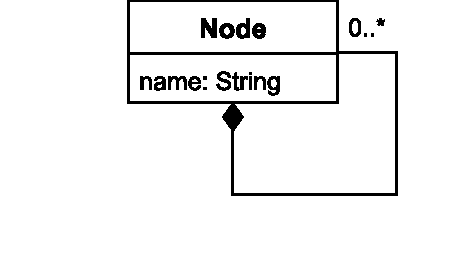
\includegraphics[width=\linewidth]{node_metamodel}
\caption{the tree metamodel (EMF/Ecore)}
\label{fig:tree_metamodel}
\end{subfigure}
\hfill
\begin{subfigure}[t]{0.32\linewidth}
\centering
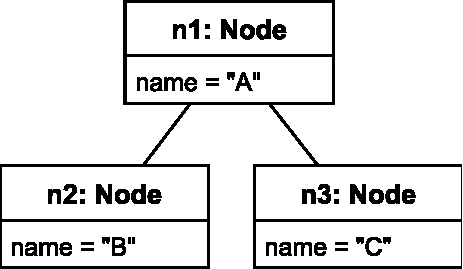
\includegraphics[width=\linewidth]{initial_chart_1}
\caption{the initial state of a tree model}
\label{fig:initial_model}
\end{subfigure}
\hfill
\begin{subfigure}[t]{0.32\linewidth}
  \centering
  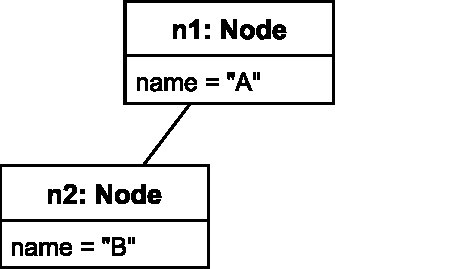
\includegraphics[width=\linewidth]{initial_chart_2}
  \caption{the eventual state after \textsf{n3} is deleted}
  \label{fig:modified_model}
\end{subfigure}
\caption{Running example of a metamodel and a conformant model.}
\label{fig:tree_example}
\end{figure}

The initial state of the model in Figure \ref{fig:initial_model} has three nodes, \textsf{n1}, \textsf{n2}, and \textsf{n3}. It was initially constructed by firstly creating the three nodes (\textsf{n1}, \textsf{n2}, and \textsf{n3}) and nodes \textsf{n2} and \textsf{n3} were added as children of \textsf{n1}. The model then was modified by deleting node \textsf{n3} producing the eventual state in Figure \ref{fig:modified_model}.

\vspace{-20pt}
\begin{minipage}[t]{0.49\linewidth}
\begin{lstlisting}[style=xmi,caption={State-based representation in simplified XMI of the tree model in Figure \ref{fig:initial_model}.},label=lst:xmimodel_0]
<Node id="n1" name="A">
  <children id="n2" name="B"/>
  <children id="n3" name="C"/>
</Node>
\end{lstlisting}
\end{minipage}
\hfill
\begin{minipage}[t]{0.49\linewidth}
\begin{lstlisting}[style=xmi,caption={State-based representation in simplified XMI of the tree model in Figure \ref{fig:modified_model}.},label=lst:xmimodel]
<Node id="n1" name="A">
  <children id="n2" name="B"/>
</Node>
\end{lstlisting}
\end{minipage}

\vspace{-20pt}
\begin{minipage}[t]{0.49\linewidth}
\begin{lstlisting}[style=eol,caption={Change-based representation of the tree model in Figure \ref{fig:initial_model}.},label=lst:cbpmodel_0]
create n1 of Node
set n1.name from null to "A"  
create n2 of Node
set n2.name from null to "B"  
create n3 of Node
set n3.name from null to "C"  
add n2 to n1.children at 0  
add n3 to n1.children at 1
\end{lstlisting}
\end{minipage}
\hfill
\begin{minipage}[t]{0.49\linewidth}
  \begin{lstlisting}[style=eol,caption={Change-based representation of the tree model in Figure \ref{fig:modified_model}.},label=lst:cbpmodel]
create n1 of Node
set n1.name from null to "A"  
create n2 of Node
set n2.name from null to "B"  
create n3 of Node
set n3.name from null to "C"  
add n2 to n1.children at 0  
add n3 to n1.children at 1
remove n3 from n1.children at 1
delete n3
\end{lstlisting}
\end{minipage}

Listings \ref{lst:xmimodel_0} and \ref{lst:xmimodel} show the simplified XMI format of the models in Figures \ref{fig:initial_model} and \ref{fig:modified_model} when they are persisted in state-based representation. Listings \ref{lst:cbpmodel_0} and \ref{lst:cbpmodel} show the change-based representation of both models respectively, using the CBP syntax introduced in Chapter \ref{ch:change_based_model_persistence}. As can be seen in both change-based representation, lines 1-6 record the creation and naming of the three nodes, and lines 7-8 record the addition of \textsf{n2} and \textsf{n3} as children of \textsf{n1}. Change-based representation in Listing \ref{lst:cbpmodel} records two additional rows since it also records the recent changes that produce the eventual state of the tree model in Figure \ref{fig:modified_model}. Lines 9-10 capture the deletion of \textsf{n3} (the \textsf{remove} command removes f \textsf{n3} from its container, and the $delete$ command completely removes \textsf{n3} from its model). Changes in a CBP representation can be uniquely identified by their line numbers.

The example model history illustrates a case where  earlier events (creating \textsf{n3} in line 5, naming it in line 6, making it a child of \textsf{n1} in line 8, removing it from the container in line 9) are superseded by a subsequent event (deletion of \textsf{n3} in line 10).  Loading of the eventual model would arguably be faster if the events in lines 5, 6, 8, 9 and 10 could be ignored.

%\vspace{-10pt}
\section{Towards Efficient Loading of Change-Based Models}
\label{sec:loading_time_optimisation}

%\vspace{-10pt}
The flowchart in Figure \ref{fig:flowchart} provides an overview of the editing lifecycle of a CBP model \cite{DBLP:conf/models/YohannisKP17}, with the proposed extensions shown as starred blocks. A model is loaded (1), edited (2) and saved (3).  During editing, the changes made to the model are recorded in a memory-based data structure, serialised and with the latest events appended at the end (4). The change events are persisted into a CBP file every time the model is saved (5). When a model is re-loaded, the current model state is recreated by replaying the events stored in the CBP file (6).

\begin{figure}[ht]
\centering
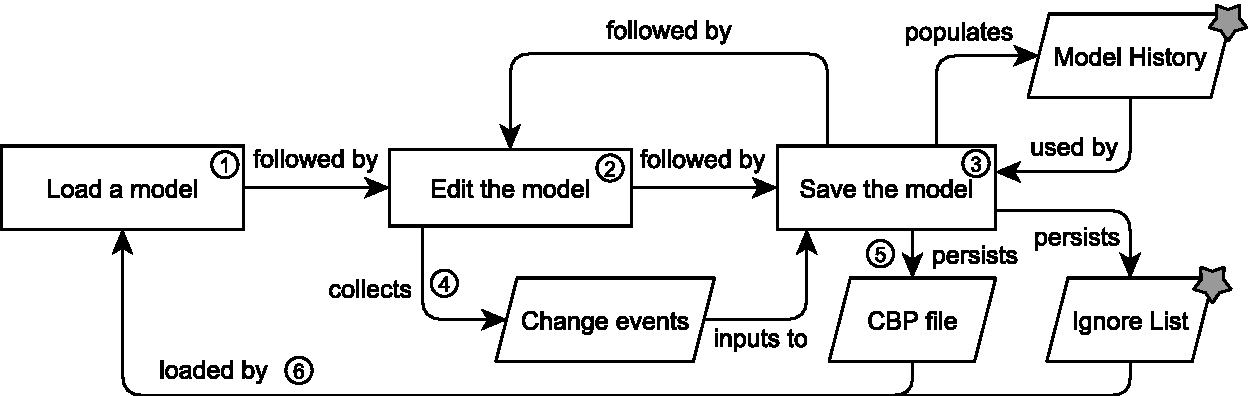
\includegraphics[width=\linewidth]{flowchart}
\caption{CBP workflow, with optimised loading elements indicated by starred blocks.}
\label{fig:flowchart}
\end{figure}

A key principle of CBP is that the editing history is immutable, as this is essential for supporting incremental model management operations. As such, superseded events cannot be simply removed from the CBP file. Therefore, the proposed approach adds two artefacts: a in-memory \textit{Model History} data structure which aggregates change events per model element, and an \textit{Ignore List} file, which persists the position (i.e. line numbers) of superseded events so that the events can be ignored the next time the model is loaded. The Ignore List is saved alongside the CBP file. The rest of this section presents how the Model History is used to detect superseded events and generate the Ignore List.

\subsection{Model History}
\label{subsec:model_history}
The Model History data structure stores events and their line numbers in a CBP representation.  The data can be used to reason about the events of a particular element and to determine which events are superseded. The line number in the CBP representation is referred as the \textit{event number}. The proposed data structure is defined in Figure \ref{fig:object_history} using a class diagram.  

A \textsf{ModelHistory} has a \textsf{URI} attribute to identify the model for which it records changes.  A \textsf{ModelHistory} can link to many \textsf{ElementHistory} objects, each identified by its \textsf{element} field which is queried from the model. An \textsf{ElementHistory} can link to many \textsf{FeatureHistories}, representing the editing histories of individual features -- either references or attributes of the element. A \textsf{FeatureHistory} has a \textsf{type} (attribute or reference) and a \textsf{name}, identifying the feature.

%\vspace{-20pt}    
\begin{figure}[ht]
\centering
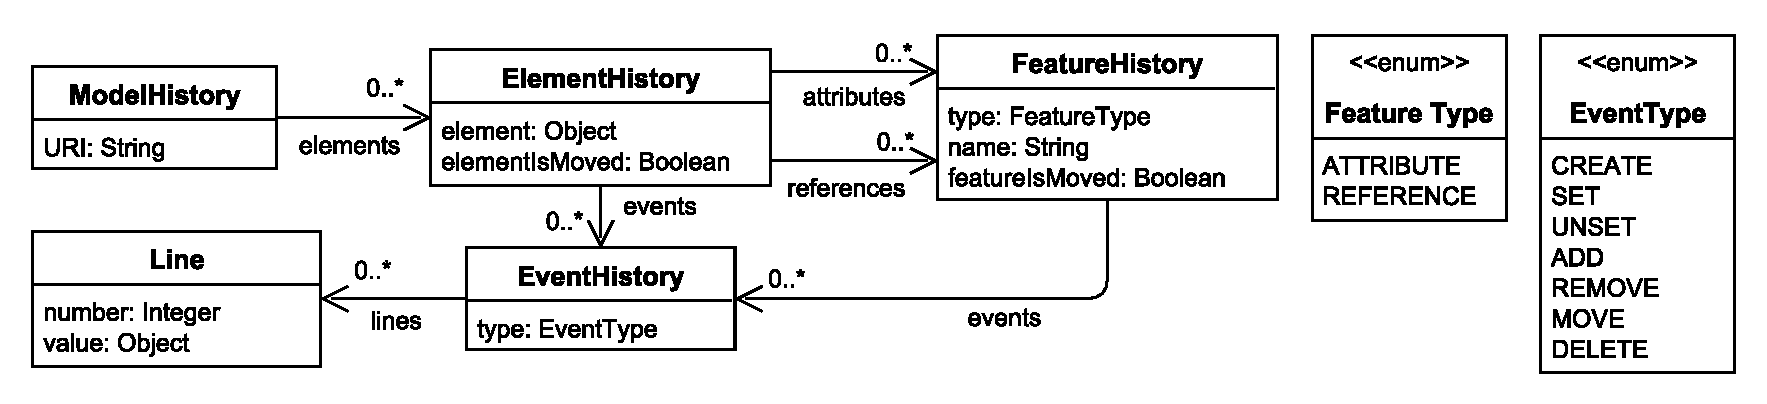
\includegraphics[width=\linewidth]{object_history}
\caption{The class model defining Model History.}
\label{fig:object_history}
\end{figure}

%\vspace{-30pt}
\begin{figure}[ht]
\centering
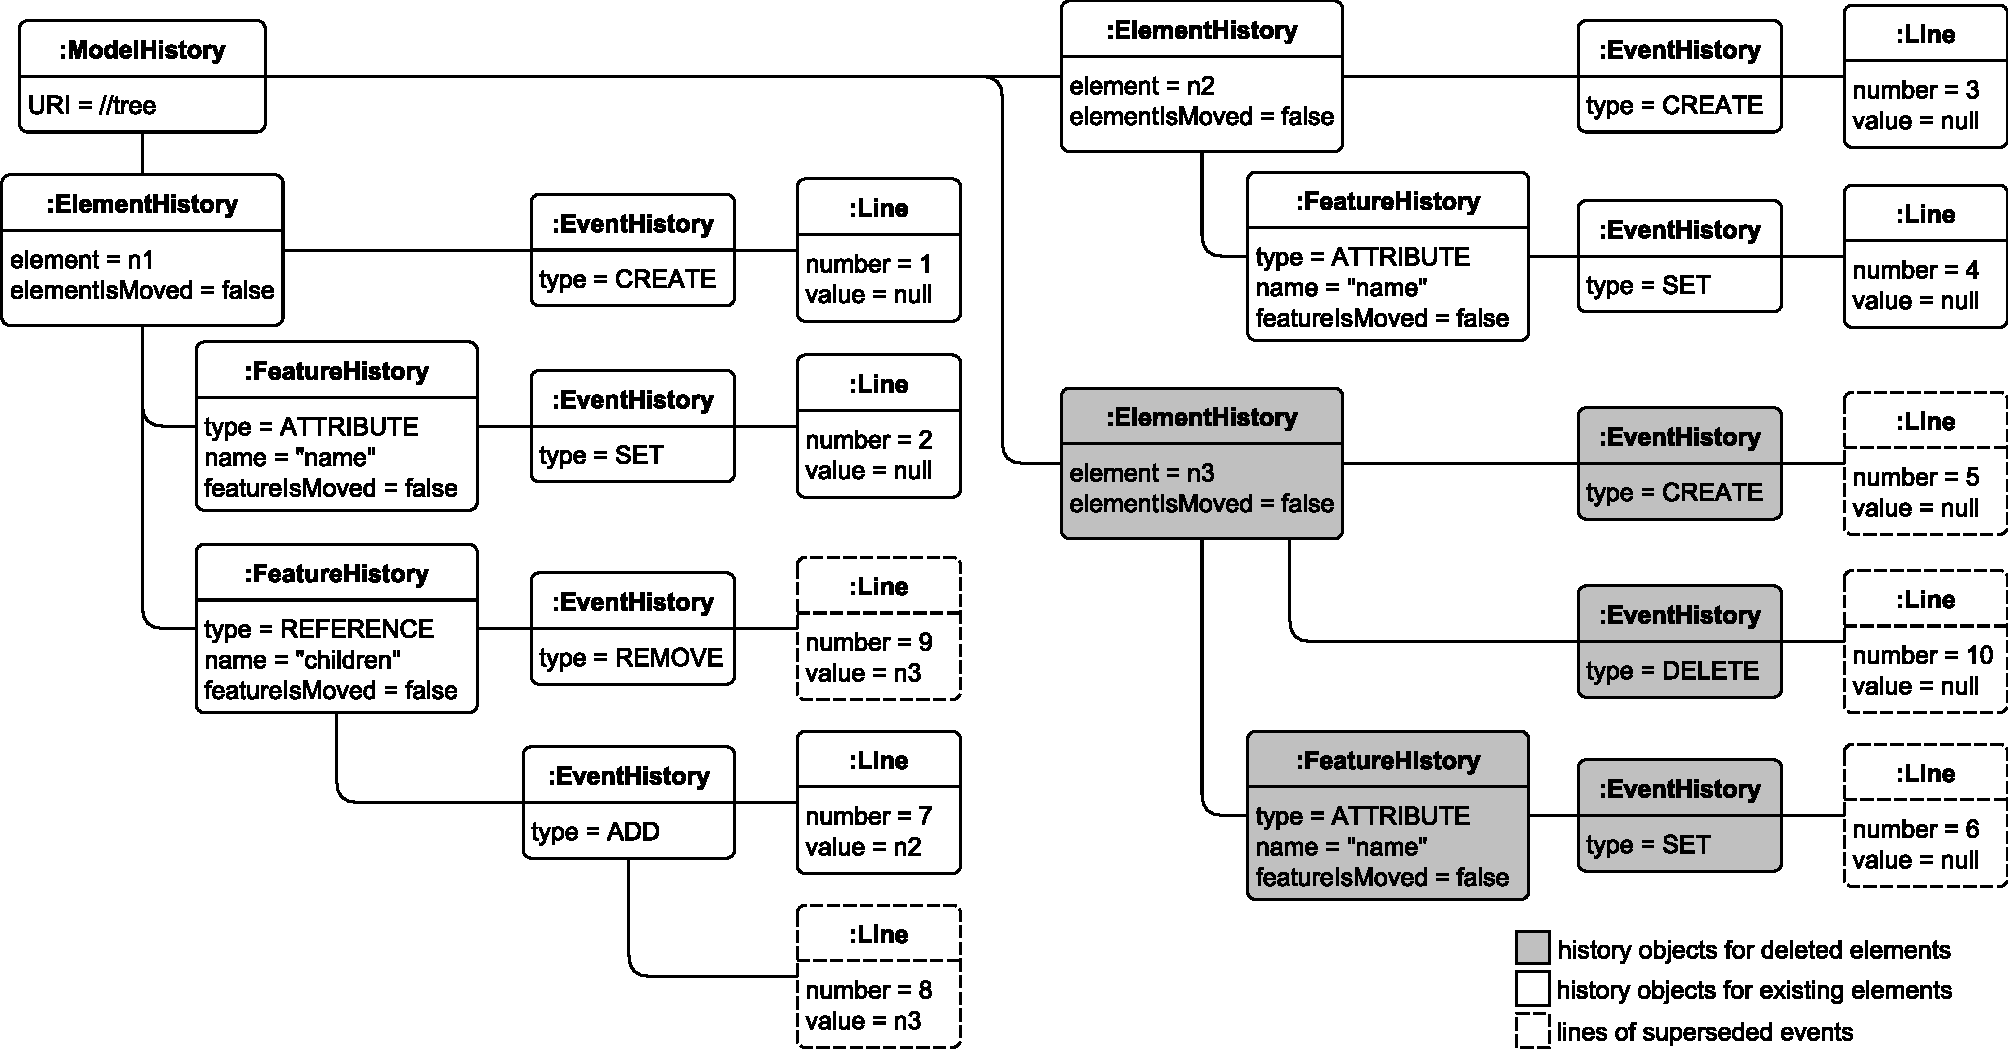
\includegraphics[width=\linewidth]{history_structure}
\caption{The object diagram of the CBP model history in Listing \ref{lst:cbpmodel}.}
\label{fig:history_structure}
\end{figure}

An \textsf{EventHistory} represents series of events of the same type; it has an attribute \textsf{type} to identify the events' type and can have many \textsf{Line}s. A \textsf{Line} has a \textsf{number} attribute, to record the event number and a \textsf{value} that records the element involved in the event (Value is only used for events with types \textsf{add}, \textsf{remove} and \textsf{move}). Each \textsf{FeatureHistory} can have many \textsf{EventHistories}, to represent the events that modify the values of the features. Each \textsf{ElementHistory} can have many \textsf{EventHistories} to represent events that affect the state of the elements (life-cycle and relations to multivalued features). Figure \ref{fig:history_structure} shows an object diagram corresponding to the model in Figure \ref{fig:object_history} that captures the model history shown in Listing \ref{lst:cbpmodel}. The grey rectangles are \textsf{History} objects related to the deleted node \textsf{n3}. The rectangles with the dashed outline are \textsf{Line} objects that represent superseded changes. 

Next, this work presents the different strategies used to identify superseded events that will be added to the Ignore List.   

%\vspace{-10pt}
\subsection{Set and Unset Events}
\label{subsec:set_and_unset_operations}
During the lifecycle of a model, a single-valued feature can have its value set (assigned) or unset many times. Each event is persisted, but only the last assigned value needs to be considered. For example, in Listing \ref{lst:set_unset_example_1}, the feature \textsf{name} is set to the value ``A'', unset, and finally set to the value ``B''.  In the final state of the model, \textsf{n1.name} = ``B''. Thus, only line 4 is significant for the model's final state and therefore lines 2 and 3 can be ignored when loading the model. For a \textsf{set} event, all preceding \textsf{set} and \textsf{unset} events can be ignored, but for an \textsf{unset} event, all \textsf{set} and \textsf{unset} events can be ignored. Executing it does not have any effect on the final state of a model if all the preceding events also have been ignored.

\vspace{-20pt}
\begin{minipage}[t]{0.49\linewidth}
\begin{lstlisting}[style=eol,caption={A CBP representation of attribute \textsf{name} assignments ended with SET.},label=lst:set_unset_example_1]
create n1 of Node
set n1.name from null to "A"
unset n1.name from "A" to null
set n1.name from null to "B"
\end{lstlisting}
\end{minipage}
\hfill
\begin{minipage}[t]{0.49\linewidth}
\begin{lstlisting}[style=eol,caption={A CBP representation of attribute \textsf{name} assignments ended with UNSET.},label=lst:set_unset_example_2]
create n1 of Node
set n1.name from null to "A"
set n1.name from null to "B"
unset n1.name from "B" to null
\end{lstlisting}
\end{minipage}

Based on the Listing \ref{lst:set_unset_example_1}, our approach creates an instance of \textsf{ElementHistory} \textsf{n1} which contains an instance of \textsf{FeatureHistory} \textsf{name}. The \textsf{FeatureHistory} \textsf{name} consists of two \textsf{EventHistory} instances, with types \textsf{set} and \textsf{unset} (the instances are named \textsf{set} and \textsf{unset} respectively for brevity). The \textsf{set} records the $Line$ instances that hold the event numbers where the \textsf{set} events, and similarly for \textsf{unset}.

From Listing \ref{lst:set_unset_example_1}, we can thus infer that \textsf{name}.\textsf{set}.\textsf{lines} = $\{2,4\}$ and \textsf{name}.\textsf{unset}. \textsf{lines} = $\{3\}$. The event numbers in both lists are used to determine that the events represented by lines 2 and 3 are superseded by that in line 4, which is a \textsf{set} event, giving an \textsf{ignoreList} = $\{2, 3\}$.  By the same process, for Listing \ref{lst:set_unset_example_2}, we can reason that \textsf{name}.\textsf{set}.\textsf{lines} = \{2,3\} and \textsf{name}.\textsf{unset}.\textsf{lines} = \{4\}.  However, this case, the highest-numbered event is an \textsf{unset}, all so line numbers are put into the ignoreList (\textsf{ignoreList} = $\{2, 3, 4\}$) (\textsf{unset} event can be ignored along with all preceding {\textsf{set} and \textsf{unset} events). 

%\vspace{-10pt}
\subsection{Add, Remove, and Move Events}\label{subsec:add_remove_and_move_operations}
For a multi-valued feature, add, remove, and move events can be called many times, to modify the feature. If an element is added to the feature, moved multiple times, and finally removed, then all the element's preceding events can be ignored, as long as the order of the feature's elements is not changed. 

Listing \ref{lst:add_move_reference} shows an example without a \textsf{move} event. In the Listing, nodes \textsf{n1}, \textsf{n2}, and \textsf{n3} are added to the \textsf{children} feature of \textsf{p} (lines 5-7), In the latest state of the model, \textsf{children} only contains \textsf{n1} and \textsf{n3}. As a result, the loading process could ignore the events that represent the \textsf{add} and \textsf{remove} events on \textsf{n1}. 

\vspace{-20pt}
\begin{lstlisting}[style=eol,caption={A CBP of add and remove operations.},label=lst:add_move_reference]
create p of Node                // children = []
create n1 of Node               // children = []
create n2 of Node               // children = []
create n3 of Node               // children = []
add n1 to p.children at 0       // children = [n1]
add n2 to p.children at 1       // children = [n1, n2]
add n3 to p.children at 2       // children = [n1, n2, n3]
remove n2 from p.children at 1  // children = [n1, n3]   
\end{lstlisting}

\vspace{-20pt}
\begin{lstlisting}[style=eol,caption={A CBP representation of add, move, and remove operations.},label=lst:add_remove_move_reference]
create p of Node                    // children = []          
create n1 of Node                   // children = []         
create n2 of Node                   // children = []         
create n3 of Node                   // children = []
add n1 to p.children at 0           // children = [n1]
add n2 to p.children at 1           // children = [n1, n2]
add n3 to p.children at 2           // children = [n1, n2, n3]
move n1 in p.children from 0 to 1   // children = [n2, n1, n3] 
remove n2 from p.children at 0      // children = [n1, n3]
\end{lstlisting}

To create the Ignore List for the Listing \ref{lst:add_move_reference}, we can deduce that \textsf{children}.\textsf{add}.\textsf{lines} = \{\{5, \textsf{n1}\}, \{6, \textsf{n2}\} \{7, \textsf{n3}\}\} (5 is the line number and \textsf{n1} is the value) and \textsf{children}.\textsf{remove}.\textsf{lines} = \{\{8, \textsf{n1}\}\}. Since \textsf{n2} is removed from its containing feature (line 8), then executing its preceding add and remove events is unnecessary. Note that we retain the \textsf{create} event (line 3) as \textsf{n2} has not been deleted from the model -- only removed from its containing feature. We can iterate through the add and move structures to identify the events on \textsf{n2} that should be removed, resulting in the \textsf{ignoreList} = \{6, 8\}.

Listing \ref{lst:add_remove_move_reference} shows an example with a \textsf{move} event\footnote{The commented parts  show the end states of \textsf{children} after each event}. A \textsf{move} event is inserted at line 8 thus makes the \textsf{remove} event of \textsf{n2}  moves to line 9. With the introduction of this \textsf{move} event, we now have the \textsf{children}.\textsf{add}.\textsf{lines} = \{\{5, \textsf{n1}\}, \{6, \textsf{n2}\} \{7, \textsf{n3}\}\}, \textsf{children}.\textsf{move}.\textsf{lines} = \{\{8, \textsf{n1}\}\}, and \textsf{children}.\textsf{remove}.\textsf{lines} = \{\{9, \textsf{n2}\}\}. In the final state of the model, the \textsf{children} should have the \textsf{n1} and \textsf{n3} in order, \textsf{children} = [n1, n3].  

However, executing the previous strategy naively leads to an erroneous final state. Using \textsf{ignoreList} = \{6, 8\} produced by the naive strategy leads to a different order of \textsf{n1} and \textsf{n3} in the final state of the model where \textsf{children} = [n3, n1] as shown by the naive optimised CBP in Listing \ref{lst:naive_add_remove_move_reference}. To overcome this problem, *$IsMoved$ flags in Figure \ref{fig:object_history} is used to sign  features and elements if they have been moved -- the flags are set to $true$. If an element's *$IsMoved$ flag is true then all of its line numbers related to \textsf{add}, \textsf{move}, \textsf{remove} events cannot be put into the \textsf{ignoreList}. The flags are set to $false$ if the feature is empty. 

\vspace{-20pt}
\begin{lstlisting}[style=eol,caption={A naive optimised CBP representation of original CBP representation in Listing \ref{lst:add_remove_move_reference} .},label=lst:naive_add_remove_move_reference]
create p of Node                    // children = []
create n1 of Node                   // children = []
create n2 of Node                   // children = []
create n3 of Node                   // children = []
add n1 to p.children at 0           // children = [n1]
add n3 to p.children at 1           // children = [n1, n3]
move n1 in p.children from 0 to 1   // children = [n3, n1]
\end{lstlisting}

\subsection{Create and Delete Events}
\label{subsec:create_and_delete_operations}

When an element is deleted, it is completely removed from the model. Therefore, all previous events ($create$, \textsf{set}, \textsf{unset}, \textsf{move}, \textsf{add}, \textsf{remove}, $delete$) on features of element can be ignored, along with all events on the element's features. For example, when node \textsf{n3} in Listing \ref{lst:cbpmodel} is deleted, the events in lines 5-6 and 8-10 are superseded. If the Listing \ref{lst:cbpmodel} is optimised -- some of its events are ignored -- when loading, it runs as if the Listing \ref{lst:cbpmodel_optimised} are executed.

\vspace{-20pt}
\begin{lstlisting}[style=eol,caption={Change-based representation of the model in Figure \ref{fig:tree_example} after removal of node \textsf{n3}.},label=lst:cbpmodel_optimised]
create n1 of Node
set n1.name from null to "A"
create n2 of Node
set n2.name from null to "B"
add n2 to n1.children at index 0
\end{lstlisting}

Using the Listing \ref{lst:cbpmodel}, we can construct the structure of histories that are related to element \textsf{n3} as follows: \textsf{n3}.$create$.\textsf{lines} = \{5\}, \textsf{n3}.\textsf{name}.\textsf{set}.\textsf{lines} = \{6\}, \textsf{n1}.\textsf{children}.\textsf{add}.\textsf{lines} = \{\{7, \textsf{n2}\}, \{8, \textsf{n3}\}\}, \textsf{n1}.\textsf{children}.\textsf{remove}.\textsf{lines} = \{\{9, \textsf{n3}\}\}, and \textsf{n3}.$delete$.\textsf{lines} = \{10\}. Thus, when element \textsf{n3} is deleted, by iterating through all these history structures, all line numbers associated with \textsf{n3} can be identified and added to \textsf{ignoreList} producing \textsf{ignoreList} = \{5 6, 8, 9, 10\} so they can be ignored in the next model loading.

\section{Evaluation}
\label{sec:evaluation_4}

This work has developed the proposed efficient loading approach on top of the original CBP implementation \cite{DBLP:conf/models/YohannisKP17,epsilonlabs2019emfcbp} and evaluated our approach's model loading performance, as well as its memory footprint and its impact on the time required to save changes made to CBP models. The evaluation was performed on Intel\textsuperscript{\textregistered} Core\textsuperscript{TM} i7-6500U CPU@2.50GHz 2.59GHz, 12GB RAM, and the Java\textsuperscript{TM} SE Runtime Environment (build 1.8.0\textunderscore162-b12).

Given that CBP is a very recent contribution and this work is not aware of any existing datasets containing real-world models expressed in a change-based format, this work has used synthetic change-based models for the experiments. The synthetic models were derived from real-world cases: the BPMN2 \cite{eclipse2017bpmn2,eclipse2018bpmn2git} and Epsilon \cite{eclipse2017epsilon,eclipse2018epsilongit} software projects, and the United States article \cite{wikipedia2018us} on Wikipedia (the article is further referred as Wikipedia). For the first two projects, for each version of the cases, MoDisco \cite{DBLP:journals/infsof/BruneliereCDM14} was used to generate a UML2 \cite{eclipse2017uml2} model that reflects its source code. For the Wikipedia article, a model that conforms to the Modisco XML metamodel \cite{eclipse2018modiscoxml} was generated. Since these cases have many versions -- represented by commits/revisions, different models of the versions can be generated, and to some degree, they reflect the time-ordered changes of the cases. The synthetic change-based model for each case was derived by comparing an initially-empty running model to different versions of the case's models sequentially. All identified differences were then reconciled by performing a unidirectional merging to the running model. All changes made to the running model during the merging process were captured and persisted into a CBP file. EMF Compare was used \cite{eclipse2017compare} to perform the comparison and merging.

Using the synthetic models, this work performed performance evaluation on loading time, saving time, and memory footprint for both loading and saving. To compare the loading time, this work ran the optimised and original (baseline) CBP algorithms to reconstruct the current state of each of the three models (the results are shown in Figure \ref{fig:loadtime}). As discussed in Section \ref{sec:loading_time_optimisation}, optimised CBP also does extra work when saving the changes to a model, in order to save time (relative to original CBP) when loading a model. To analyse the performance effect of optimisation activities, we, therefore, compared the overall time required to save a new version of the models described above, after one single change has been made (The results are shown in Figure \ref{fig:savetime}). This work also compared the memory footprints for both loading and saving since the optimised CBP approach also requires the maintenance of an additional in-memory data structure that keeps track of element and feature editing histories (see Figure \ref{fig:loadmemory} and \ref{fig:savememory} for the results). 

For each combination of dimensions (loading time, saving time, loading memory footprint, saving memory footprint),  persistence types (original CBP, optimised CBP, and XMI), and cases (BPMN2, Epsilon, and Wikipedia), we performed measurement 22 times. The results of the measurement enabled us to perform the Welch's t-test \cite{welch1947ttest} to find the significance of the comparisons for each case. This evaluation used a significance level of 5\%. If t-test' $p$-$value$ $<$ 0.05, the null hypothesis -- the $means$ of the compared persistence types are equal ($H_0$) -- is rejected and the alternative hypothesis -- the $means$ of the compared persistence types are not equal ($H_1$) -- is accepted.

For loading and saving time, this work measured the delta time required to complete the loading and saving. For memory footprint, this work measured the delta of memory used before and after loading and saving completes. The results are presented below.

\subsection{Data Description}
\label{subsec:data_description}

\begin{table} [ht]
\centering
\caption{Description of change-based models generated for evaluation.}
\label{table:data_description}
\begin{tabular}{>{\centering\arraybackslash}p{1.5cm}>{\centering\arraybackslash}p{1.7cm}>{\centering\arraybackslash}p{1.7cm}>{\centering\arraybackslash}p{1.6cm}
>{\centering\arraybackslash}p{1.5cm}>{\centering\arraybackslash}p{2cm}}
\hline 
\textbf{Model} & \textbf{Total Events} & \textbf{Ignored Events} & \textbf{Elements} & \textbf{Total Versions} & \textbf{Processed Versions} \\
\hline
BPMN2 & \multicolumn{1}{r}{1.2 million} & \multicolumn{1}{r}{1.1 million} & \multicolumn{1}{r}{62,062} & \multicolumn{1}{r}{192} & \multicolumn{1}{r}{192 (100.0\%)} \\
Epsilon & \multicolumn{1}{r}{2.6 million} & \multicolumn{1}{r}{1.8 million} & \multicolumn{1}{r}{79,459} & \multicolumn{1}{r}{3,037} & \multicolumn{1}{r}{727 (23.9\%)} \\
Wikipedia & \multicolumn{1}{r}{11.5 million} & \multicolumn{1}{r}{7.8 million} & \multicolumn{1}{r}{12,144} & \multicolumn{1}{r}{37,996} & \multicolumn{1}{r}{3,100 (8.2\%)} \\
\hline 
\end{tabular}
\end{table}

Table \ref{table:data_description} summarises events, elements and saved versions for the Epsilon, BPMN2, and Wikipedia cases. $Total$ $Events$ is the numbers of events that were produced by our approach in generating a change-based model for each case.  $Ignored$ $Events$ is the number of superseded events that do not need to be replayed when reloading the models. $Elements$ is the number of elements contained in each model. $Total$ $Versions$ is the number of commits/revisions made to the cases, taken from the git repositories or Wikipedia at the time this evaluation performed. $Processed$ $Versions$ is the number of commits/revisions that were processed to produce change-based models: since the comparison between versions takes considerable time, not all versions are processed here.

\subsection{Model Loading Time}
\label{subsec:loading_time_test}
This section presents the results of the loading time measurement of change-based models for each pair of the persistence types and cases, and the t-test results of their comparisons (Table \ref{table:ttest_results_loadtime} and Figure \ref{fig:loadtime}). 

\begin{table}[ht]
\footnotesize
\centering
\caption{The t-test results of loading time comparison between original CBP (CBP), optimised CBP (OCBP), and XMI.}
\label{table:ttest_results_loadtime}
\begin{tabular}
{|p{0.08\textwidth}p{0.08\textwidth}p{0.09\textwidth}|p{0.18\textwidth}p{0.10\textwidth}p{0.06\textwidth}p{0.08\textwidth}|}
\hline 
% BPMN2 Load Time
Group & Mean & SD & Comparison & t  & df & p-value \\  
\hline 
\multicolumn{3}{|c|}{\textbf{BPMN2 Load Time ($s$)}} & \multicolumn{4}{c|}{\textbf{BPMN2 Load Time}} \\ 
CBP & 5.81 & 0.08 & CBP vs. XMI & 315.95    &21.46 & $<$ 0.05 \\  
OCBP & 3.02 & 0.13 & CBP vs. OCBP & 87.67 & 35.10  & $<$ 0.05 \\  
XMI & 0.47 & 0.47 & OCBP vs. XMI & 93.86    & 21.18  & $<$ 0.05 \\ 
\hline 

% EPSILON Load Time
\multicolumn{3}{|c|}{\textbf{Epsilon Load Time ($s$)}} & \multicolumn{4}{c|}{\textbf{Epsilon Load Time}} \\
CBP & 16.60    & 0.23 &  CBP vs. XMI & 324.18   &22.78 & $<$ 0.05 \\
OCBP &  8.28  &  0.09 & CBP vs. OCBP & 160.06 & 27.48 & $<$ 0.05 \\  
XMI & 0.60   & 0.05 & OCBP vs. XMI & 354.52   &42.06  & $<$ 0.05 \\ 
\hline 

% WIKIPEDIA Load Time
\multicolumn{3}{|c|}{\textbf{Wiki Load Time ($s$)}} & \multicolumn{4}{c|}{\textbf{Wikipedia Load Time}} \\
CBP & 34.23   & 0.145 & CBP vs. XMI & 1,110.10   &21.00 & $<$ 0.05 \\ 
OCBP & 26.14  & 1.583 & CBP vs. OCBP &  23.90 &21.35 & $<$ 0.05 \\ 
XMI &  0.02  & 0.001 & OCBP vs. XMI & 77.37   & 21.00 & $<$ 0.05 \\ 
\hline
\end{tabular}
\justify
$Mean$ = average, $SD$ = standard deviation, $t$ = t-test's $t$-$value$, $df$ = degree of freedom, $p$-$value$ = significance, $s$ = the unit is seconds
\end{table}

\begin{figure}[ht]
  \begin{subfigure}{0.325\textwidth}
    \centering
    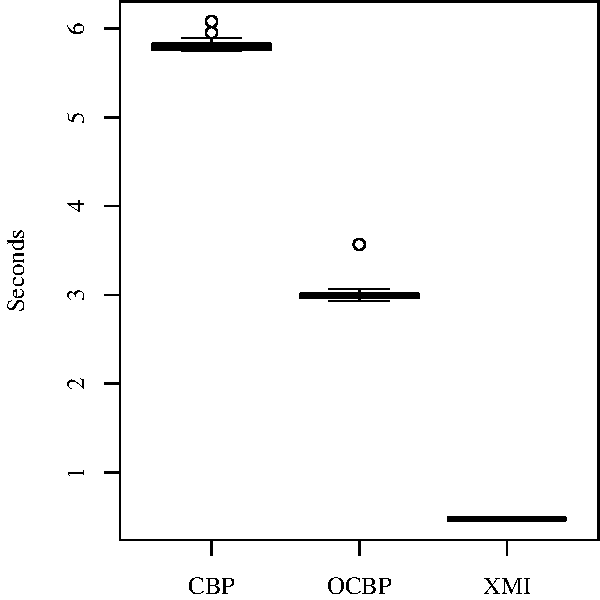
\includegraphics[width=\linewidth]{images/ol_load_time_bpmn2}
    \caption{BPMN2}
    \label{fig:load_time_bpmn2}
  \end{subfigure}
  \hfill
  \begin{subfigure}{0.325\textwidth}
    \centering
    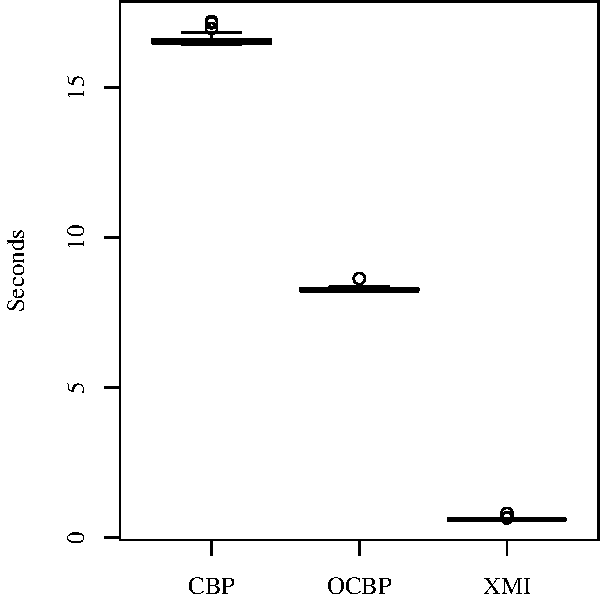
\includegraphics[width=\linewidth]{images/ol_load_time_epsilon}
    \caption{Epsilon}
    \label{fig:load_time_epsilon}
  \end{subfigure}
  \hfill
  \begin{subfigure}{0.325\textwidth}
    \centering
    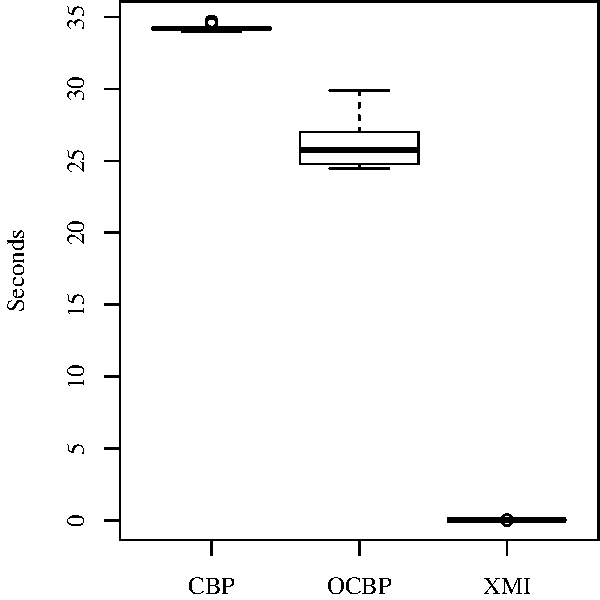
\includegraphics[width=\linewidth]{images/ol_load_time_wikipedia}
    \caption{Wikipedia}
    \label{fig:load_time_wikipedia}
  \end{subfigure}
  \caption{Results for loading a model in original CBP (CBP), optimised CBP (OCBP), and for loading a state-based (XMI) representation.}
  \label{fig:loadtime}
\end{figure}

These loading times show a considerable time saving for optimised CBP: BPMN2 was 48.02\% faster, Epsilon 50.12\% faster, and the Wikipedia page 23.63\% faster than in the original CBP implementation (all optimised CBP's $means$ are  smaller than all original CBP's $means$), which has a positive correlation to the number of ignored events. All the t-test results also show that loading times for all the persistence types are significantly different (all the $p$-$values$ $<$ 0.05). 

For reference, this work also compared CBP loading with the execution time for loading the equivalent state-based model in XMI. Figure \ref{fig:loadtime} shows that, even with the improvements delivered by the new algorithm, loading change-based models is still significantly slower than loading a state-based model (all XMI's means are smaller than other persistence types' means).

\subsection{Model Saving Time}
\label{subsec:saving_time_test}
This subsection presents the results of the saving time measurement of change-based models for each pair of the persistence types and cases, and the t-test results of their comparisons (Table \ref{table:ttest_results_savetime} and Figure \ref{fig:savetime}). As discussed in \cite{DBLP:conf/models/YohannisKP17}, CBP loading time penalties are balanced against the benefits that CBP brings, in terms of  persisting changes (saving time).

\begin{table}[ht]
\footnotesize
\centering
\caption{The t-test results of saving time comparison between original CBP (CBP), optimised CBP (OCBP), and XMI.}
\label{table:ttest_results_savetime}
\begin{tabular}
{|p{0.08\textwidth}p{0.08\textwidth}p{0.09\textwidth}|p{0.18\textwidth}p{0.10\textwidth}p{0.06\textwidth}p{0.08\textwidth}|}
\hline 

% BPMN2 Save Time
Group & Mean & SD & Comparison & t  & df & p-value \\
\hline 
\multicolumn{3}{|c|}{\textbf{BPMN2 Save Time ($s$)}} & \multicolumn{4}{c|}{\textbf{BPMN2 Save Time}}\\
CBP & 0.00097    & 123e-5 & CBP vs. XMI &  -175.58    & 22.01 & $<$ 0.05 \\  
OCBP & 0.00081   & 12e-5 & CBP vs. OCBP & 0.62 & 21.38  & 0.54 \\  
XMI & 0.30122   & 793e-5 & OCBP vs. XMI & -177.76    & 21.01  & $<$ 0.05 \\ 
\hline 

% EPSILON Save Time
\multicolumn{3}{|c|}{\textbf{Epsilon Save Time ($s$)}} & \multicolumn{4}{c|}{\textbf{Epsilon Save Time}}\\
CBP & 0.00069    & 3.4e-5 &  CBP vs. XMI & -6.01   &21.00 & $<$ 0.05 \\
OCBP & 0.00080   & 8.0e-5 & CBP vs. OCBP & 160.06 & 28.24 & $<$ 0.05 \\  
XMI & 0.40025   & 595e-5 & OCBP vs. XMI & -314.80  & 21.01  & $<$ 0.05 \\ 
\hline 

% WIKIPEDIA Save Time
\multicolumn{3}{|c|}{\textbf{Wiki Save Time ($s$)}} & \multicolumn{4}{c|}{\textbf{Wikipedia Save Time}}\\
CBP & 0.00071     & 4.9e-5 & CBP vs. XMI &  -46.19   & 21.08 & $<$ 0.05 \\ 
OCBP &0.00075   &  4.1e-5 & CBP vs. OCBP &   -3.48 & 40.77 & $<$ 0.05 \\ 
XMI &  0.01195   & 114e-5 & OCBP vs. XMI &  -46.01  & 21.06 & $<$ 0.05 \\ 
\hline
\end{tabular}
\justify
$Mean$ = average, $SD$ = standard deviation, $t$ = t-test's $t$-$value$, $df$ = degree of freedom, $p$-$value$ = significance, $s$ = the unit is seconds
\end{table}



As shown in Table \ref{table:ttest_results_savetime} and Figure \ref{fig:savetime}, the performance of the two CBP implementations is not very different. Since the significance level is 5\%, only the BPMN2 case that fails. However, the difference between the $means$ of its original CBP (0.97 ms) and optimised CBP (0.81 ms) is small. This indicates that the cost of the extra work in the optimised CBP algorithm is negligible. On the other hand, both CBP implementations are significantly faster at saving changes than state-based XMI (the $means$ of both CBP implementations are smaller than XMI's $means$, and both CBP implementations have $p$-$values$ $<$ 0.05 when compared to XMI). This is expected, as the CBP implementations only need append the last changes to the existing model file (their performance is thus relative to the number of changes since the last save), while the XMI implementation needs to reconstruct an XML document for the entire state of the model, and replaces the contents of the model file every time (and hence its performance is relative to the size of the entire model). 

\begin{figure}[ht]
\begin{subfigure}{0.325\textwidth}
\centering
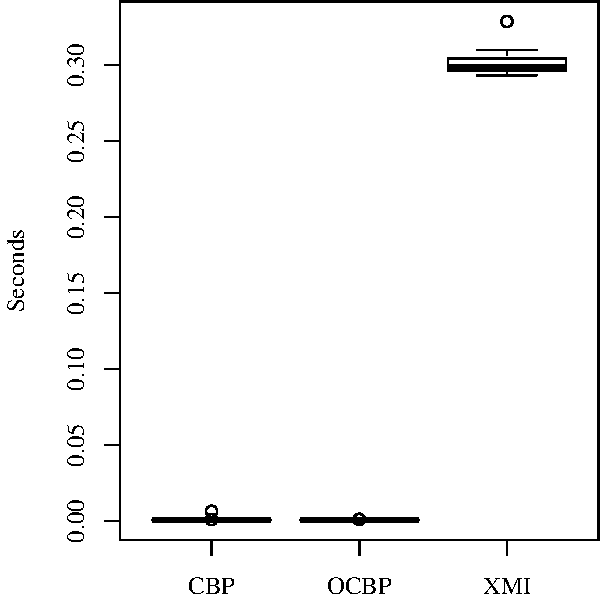
\includegraphics[width=\linewidth]{images/ol_save_time_bpmn2}
\caption{BPMN2}
\label{fig:save_time_bpmn2}
\end{subfigure}
\hfill
\begin{subfigure}{0.325\textwidth}
\centering
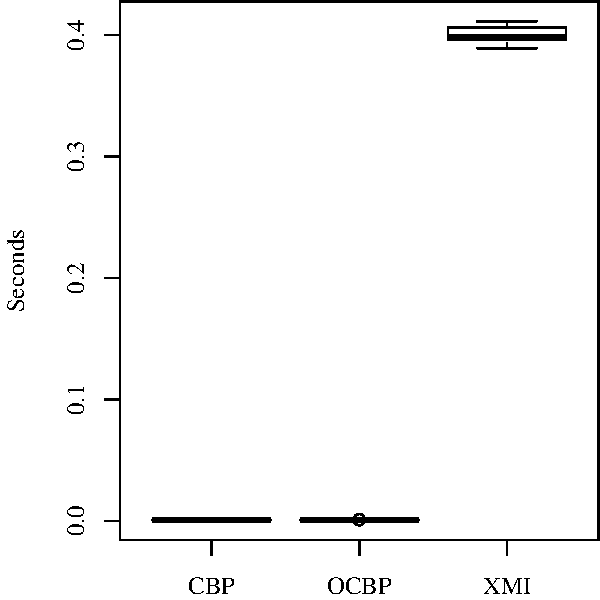
\includegraphics[width=\linewidth]{images/ol_save_time_epsilon}
\caption{Epsilon}
\label{fig:save_time_epsilon}
\end{subfigure}
\hfill
\begin{subfigure}{0.325\textwidth}
\centering
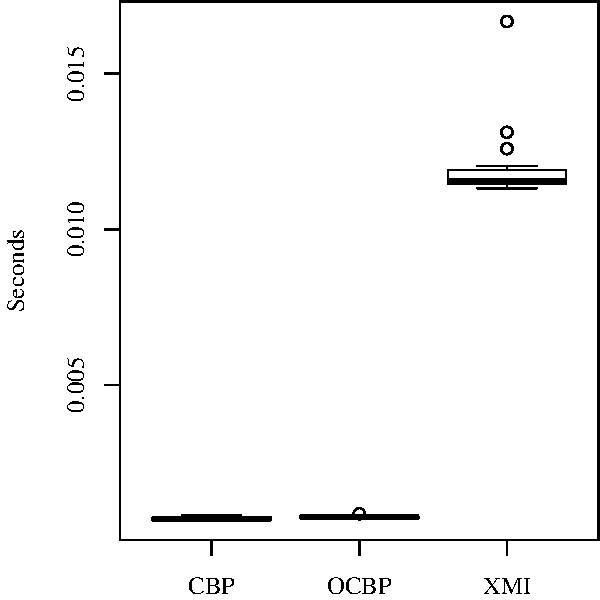
\includegraphics[width=\linewidth]{images/ol_save_time_wikipedia}
\caption{Wikipedia}
\label{fig:save_time_wikipedia}
\end{subfigure}
\caption{A comparison on time required for persisting an event between original CBP (CBP), optimised CBP (OCBP), and XMI.}
\label{fig:savetime}
\end{figure}


%\vspace{-10pt}
\subsection{Memory Footprint}
\label{subsec:memory_consumption}

\begin{table}[t]
\footnotesize
\centering
\caption{The t-test results of memory footprint comparison after loading a model between original CBP (CBP), optimised CBP (OCBP), and XMI.}
\label{table:ttest_results_load_memory}
\begin{tabular}
{|p{0.08\textwidth}p{0.08\textwidth}p{0.09\textwidth}|p{0.18\textwidth}p{0.10\textwidth}p{0.06\textwidth}p{0.08\textwidth}|}
\hline 

% BPMN2 Load Memory
Group & Mean & SD & Comparison & t  & df & p-value \\
\hline 
\multicolumn{3}{|c|}{\textbf{BPMN2 Load Memory ($M$)}} & \multicolumn{4}{c|}{\textbf{BPMN2 Load Memory}} \\
CBP & 9.76     & 76.0e-4 & CBP vs. XMI &  4,392.5   & 21.22 & $<$ 0.05 \\  
OCBP & 22.36   & 0.015 & CBP vs. OCBP & -3,695.7 & 32.28  & $<$ 0.05 \\  
XMI &  2.63   & 5.5e-4 & OCBP vs. XMI &  6,572.4    & 21.06  & $<$ 0.05 \\ 
\hline 

% EPSILON Load Memory
\multicolumn{3}{|c|}{\textbf{Epsilon Load Memory ($M$)}} & \multicolumn{4}{c|}{\textbf{Epsilon Load Memory}} \\
CBP &15.74    & 1.248 &  CBP vs. XMI & 28.16   &  41.99 & $<$ 0.05 \\
OCBP & 43.15   & 0.056 & CBP vs. OCBP & -102.9 &21.08 & $<$ 0.05 \\  
XMI & 5.05   & 1.271 & OCBP vs. XMI & 140.49  & 21.08  & $<$ 0.05 \\ 
\hline 

% WIKIPEDIA Load Memory
\multicolumn{3}{|c|}{\textbf{Wiki Load Memory ($M$)}} & \multicolumn{4}{c|}{\textbf{Wikipedia Load Memory}} \\
CBP & 2.29  & 2.4e-4 & CBP vs. XMI &   4,523.5   & 25.16 & $<$ 0.05 \\ 
OCBP & 126.48 & 0.29 & CBP vs. OCBP &   -2,009.3 & 21.00 & $<$ 0.05 \\ 
XMI &  1.52  & 7.6e-4 & OCBP vs. XMI &  2,021.8  & 21.00 & $<$ 0.05 \\ 
\hline
\end{tabular}
\justify
$Mean$ = average, $SD$ = standard deviation, $t$ = t-test's $t$-$value$, $df$ = degree of freedom, $p$-$value$ = significance, $M$ = the unit is megabytes
\end{table}

\begin{figure}[ht]
  \begin{subfigure}{0.325\textwidth}
    \centering
    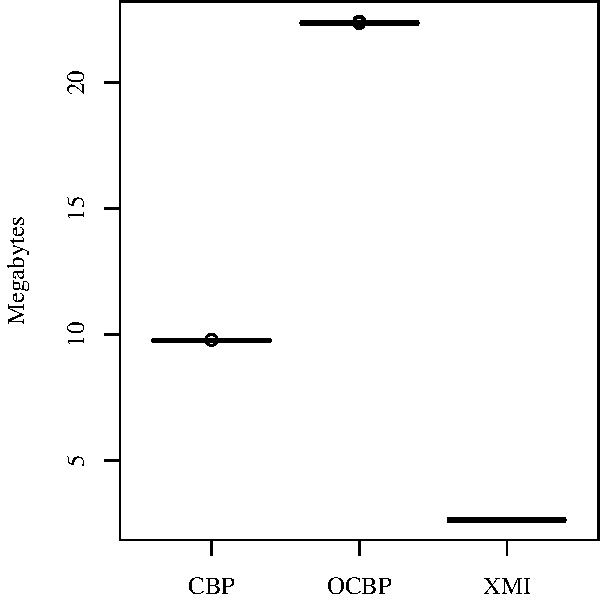
\includegraphics[width=\linewidth]{images/ol_load_memory_bpmn2}
    \caption{BPMN2}
    \label{fig:load_memory_bpmn2}
  \end{subfigure}
  \hfill
  \begin{subfigure}{0.325\textwidth}
    \centering
    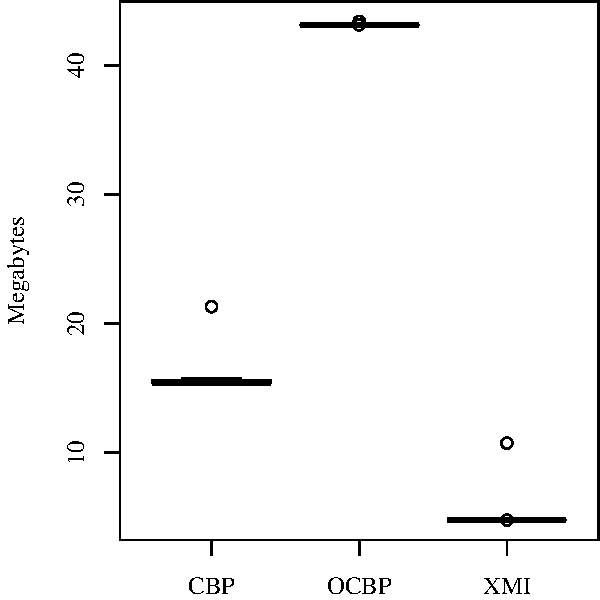
\includegraphics[width=\linewidth]{images/ol_load_memory_epsilon}
    \caption{Epsilon}
    \label{fig:load_memory_epsilon}
  \end{subfigure}
  \hfill
  \begin{subfigure}{0.325\textwidth}
    \centering
    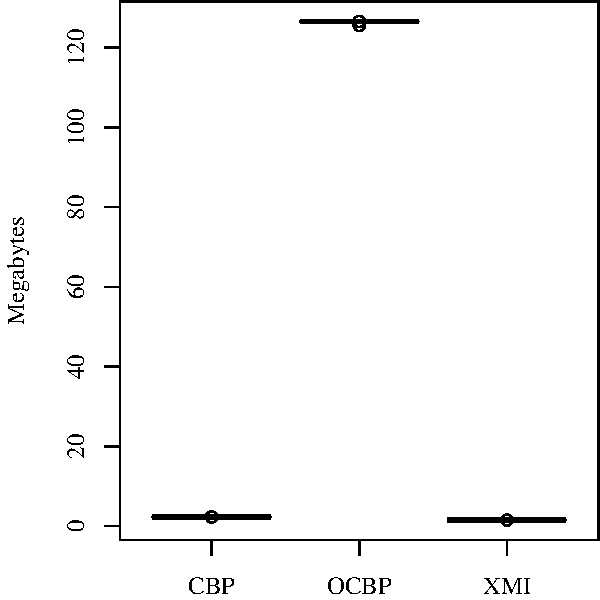
\includegraphics[width=\linewidth]{images/ol_load_memory_wikipedia}
    \caption{Wikipedia}
    \label{fig:load_memory_wikipedia}
  \end{subfigure}
  \caption{A comparison on memory footprint after loading a model between original CBP (CBP), optimised CBP (OCBP), and XMI.}
  \label{fig:loadmemory}
\end{figure}

%------------------------------

\begin{table}[ht]
\footnotesize
\centering
\caption{The t-test results of memory footprint comparison after saving an event between original CBP (CBP), optimised CBP (OCBP), and XMI.}
\label{table:ttest_results_save_memory}
\begin{tabular}
{|p{0.08\textwidth}p{0.08\textwidth}p{0.09\textwidth}|p{0.18\textwidth}p{0.10\textwidth}p{0.06\textwidth}p{0.08\textwidth}|}
\hline 

% BPMN2 Save Memory
Group & Mean & SD & Comparison & t  & df & p-value \\
\hline 
\multicolumn{3}{|c|}{\textbf{BPMN2 Save Memory ($M$)}} & \multicolumn{4}{c|}{\textbf{BPMN2 Save Memory}} \\
CBP &0.0023    & 6.3e-5 & CBP vs. XMI &  -489,170    & 41.49 & $<$ 0.05 \\  
OCBP &0.0029    & 80e-5 & CBP vs. OCBP & -3.22 & 21.26 & $<$ 0.05 \\
XMI & 8.84   & 5.6e-5 & OCBP vs. XMI & -51,180    &  21.21  & $<$ 0.05 \\ 
\hline 

% EPSILON Save Memory
\multicolumn{3}{|c|}{\textbf{Epsilon Save Memory ($M$)}} & \multicolumn{4}{c|}{\textbf{Epsilon Save Memory}}\\
CBP & 0.0025    & 18.8e-6 &  CBP vs. XMI & -4.3e\texttt{+}6   & 21.00 & $<$ 0.05 \\
OCBP & 0.0031    & 279.9e-6 & CBP vs. OCBP & -10.131 & 21.19 & $<$ 0.05 \\ %1.41e-09 \\  
XMI & 17.61   & 2.4e-6 & OCBP vs. XMI & -295,090  &21.00  & $<$ 0.05 \\ 
\hline 

% WIKIPEDIA Save Memory
\multicolumn{3}{|c|}{\textbf{Wiki Save Memory ($M$)}} & \multicolumn{4}{c|}{\textbf{Wikipedia Save Memory}} \\
CBP & 0.0025  &1.9e-5 & CBP vs. XMI &  -391,970   & 40.52 & $<$ 0.05 \\ 
OCBP &  0.0028   & 84.1e-5 & CBP vs. OCBP &  -1.75 & 21.02 &  0.094 \\ 
XMI &  2.0194   & 1.5e-5 & OCBP vs. XMI &  -11,245  & 21.01 & $<$ 0.05 \\ 
\hline
\end{tabular}
\justify
$Mean$ = average, $SD$ = standard deviation, $t$ = t-test's $t$-$value$, $df$ = degree of freedom, $p$-$value$ = significance, $M$ = the unit is megabytes
\end{table}

\begin{figure}[ht]
  \begin{subfigure}{0.325\textwidth}
    \centering
    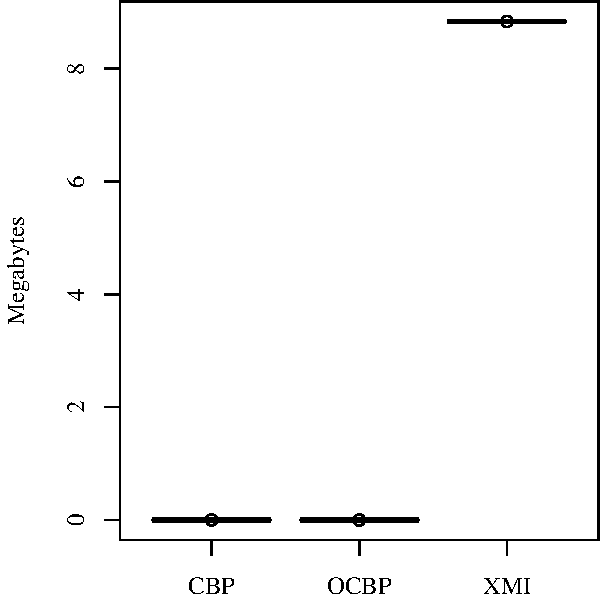
\includegraphics[width=\linewidth]{images/ol_save_memory_bpmn2}
    \caption{BPMN2}
    \label{fig:save_memory_bpmn2}
  \end{subfigure}
  \hfill
  \begin{subfigure}{0.325\textwidth}
    \centering
    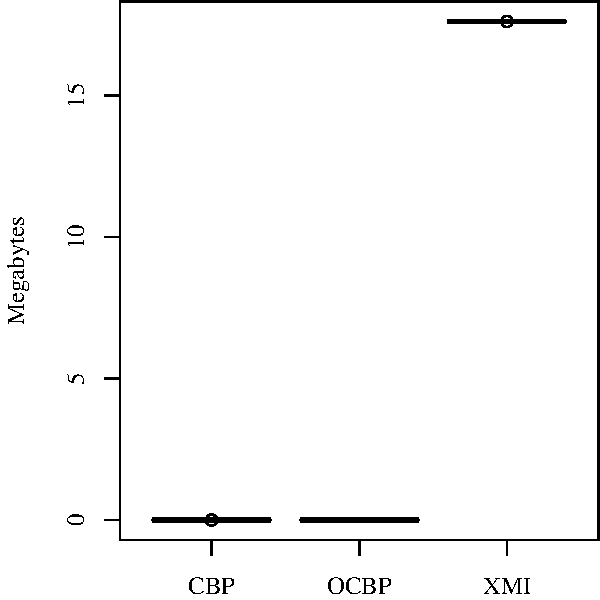
\includegraphics[width=\linewidth]{images/ol_save_memory_epsilon}
    \caption{Epsilon}
    \label{fig:save_memory_epsilon}
  \end{subfigure}
  \hfill
  \begin{subfigure}{0.325\textwidth}
    \centering
    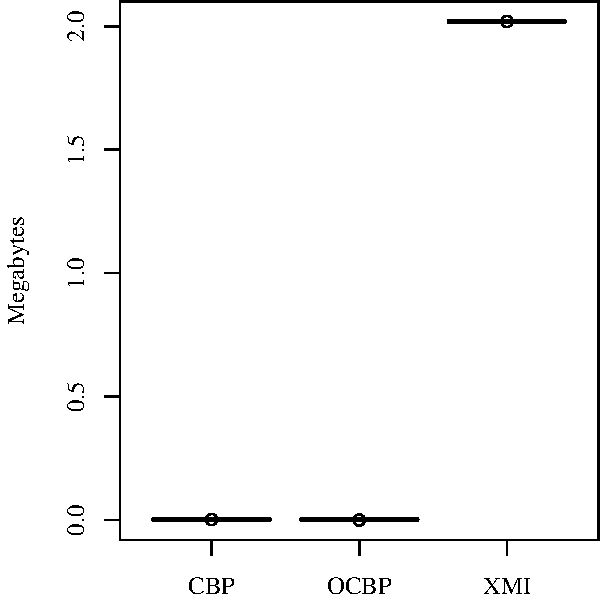
\includegraphics[width=\linewidth]{images/ol_save_memory_wikipedia}
    \caption{Wikipedia}
    \label{fig:save_memory_wikipedia}
  \end{subfigure}
  \caption{A comparison on memory footprint after persisting an event between CBP, optimised CBP, and XMI.}
  \label{fig:savememory}
\end{figure}

Using the models from the three cases, the memory footprint after loading models are presented in Table \ref{table:ttest_results_load_memory} and Figure \ref{fig:loadmemory}, and the memory footprint after persisting single changes are displayed in Table \ref{table:ttest_results_save_memory} and Figure \ref{fig:savememory}. The results show the significant memory overhead of the extra data structure when loading models (all the $means$ of optimised CBP are greater than all the $means$ of original CBP and all comparisons between both CBPs show $p$-$values$ $<$ 0.05, Table \ref{table:ttest_results_load_memory}). Both CBPs are also outperformed by XMI in terms of memory footprint when loading models (all the $means$ of XMI are smaller than all the $means$ of both CBPs and all comparisons against XMIs show all $p$-$values$ $<$ 0.05, Table \ref{table:ttest_results_load_memory}). In loading, XMI uses significantly less memory than the optimised CBP representation and performs slightly better than the original CBP.   

In terms of saving, both CBP implementations persist a single change faster than XMI indicated by their $means$ that are smaller than the $means$ of XMI, and all the CBPs' t-tests with XMI show that their differences are significant at $p$-$value$ $<$ 0.05 (Table \ref{table:ttest_results_save_memory}). The optimised CBP has a larger memory footprint than the original CBP since the means of the optimised CBP for all cases are greater than the means of the original CBP. However, their memory footprints are not very different. Even though the BPMN2 and Epsilon cases have $p$-$values$ $<$ 0.05, the differences of the $means$ of their original and optimised CBPs are small, and the Wikipedia case also shows $p$-$value$ $>$ 0.05 on its original CBP vs. optimised CBP comparison.   

\subsection{Discussion}
\label{sec:discussion}
For the original CBP loading, the total time required to load a model is $T_{CBP}$ = $T_E$ + $T_O$, where $T_E$ is the total time required to complete executing all events, and $T_O$ is the total time needed to complete other required routines (e.g. initialisation, reading files). For the optimised CBP loading, the total time to load a change-based model is reduced by the total time saved-up by ignoring superseded events $T_I$, that is $T_{OCBP}$ = $T_E$ + $T_O$ $-$ $T_I$. Thus, it is expected that optimised CBP can load a model faster than original CBP. This statement is in accordance with our finding in Section \ref{subsec:loading_time_test} that the total saved-up loading time corresponds to the number of ignored events. However, it still requires more investigation to determine the degree of their correlation, which will be addressed in our future work.

%\vspace{-5pt}
\section{Conclusions}
\label{sec:conclusions_4}
Change-based persistence can be slow when it comes to loading a model since its change records have to be replayed. This study has optimised the loading of change-based persistence by only replaying change events that affect the eventual state of a model. In other words, the replay ignores change events that are superseded by later change events.
 
This chapter has proposed an efficient algorithm and supporting data structures for the proposed optimisation. Performance is evaluated on synthesised models, with comparison against the unoptimised change-based implementation, and state-based XMI. Compared to the unoptimised change-based persistence, the optimised version shows considerable savings in terms of loading time with a negligible impact on saving time, but at the cost of a higher memory footprint. However, in terms of loading time and memory footprint, XMI outperforms both approaches but is much less efficient in saving changes. 

This chapter also has addressed the first research question of this study partially, \textbf{How can models be effectively persisted in a change-based format, and how does change-based persistence perform, compared to state-based persistence on loading and saving models?} (RQ1). Based on the evaluation results, we can identify that the performance of change-based persistence on loading models is poor compared state-based persistence. Even though it has been optimised by ignoring replaying change events that superseded by their subsequent change events, it is still significantly outperformed by loading models from their state-based persistence. It also suffers greatly on memory footprint because of the dedicated data structure employed to track change events. In terms of saving, change-based persistence shows more favourable results compared to state-based persistence since we only need to persist the recent changes applied to a model rather than saving the entire model. This condition is very favourable when we work with large models in their mature stage where only small changes occur. 


\chapter{Hybrid Model Persistence}
\label{ch:hybrid_model_persistence}

Reconstructing the state of a change-based model by replaying its editing history every time the model needs to be queried or modified can get increasingly expensive as the model grows in size. In Chapter \ref{ch:optimised_loading}, we proposed a method to speed up the reconstruction by not replaying change events that do not have any effect to the eventual states of a model. However, the method is still substantially outperformed by loading a model directly from its state-based persistence. Thus, in this chapter we report on a novel approach that integrates change-based and state-based model persistence mechanisms in a hybrid model persistence approach that delivers the best of both worlds. This Chapter presents the design of the hybrid model persistence approach and reports on its impact on time and memory footprint for model loading, saving, and storage space usage.

\section{Introduction}
\label{sec:introduction_5}
Saving models in change-based persistence (CBP) comes at the cost of ever-growing model files \cite{DBLP:conf/edoc/KoegelHLHD10,DBLP:journals/entcs/RobbesL07} since all changes (even deleting model elements) are recorded in an editing log, which naturally leads to longer loading times \cite{mens2002state}. 
In Chapter \ref{ch:optimised_loading}, we proposed a method to speed up the reconstruction by not replaying change events that do not have any effect to the eventual state of a model. However, the method is still substantially out performed by loading a model directly from its state-based persistence. Thus, this chapter proposes another solution to address the issue by introducing the concept of hybrid persistence of models. In hybrid model persistence the change-based representation is augmented with a state-based representation (which can be fully derived from the change-based representation) of the latest state of the model which is used to speed up model loading and querying.

This Chapter is structured as follows. Section \ref{sec:change_and_state_based_model_persistence} introduces the concept of change-based model persistence and recent work on state-based model persistence. Sections \ref{sec:hybrid_model_persistence} and \ref{sec:implementation} present the proposed approach to hybrid model persistence and its implementation. Sections \ref{sec:evaluation_5} and \ref{sec:discussion_5} present and discuss experimental results and evaluation. Section \ref{sec:conclusions_5} concludes this Chapter.

\section{Comparing Change and State-based Model Persistence}
\label{sec:change_and_state_based_model_persistence}
Table \ref{table:persistence_comparsion} summarises the benefits (+) and drawbacks (-) of change and state-based model persistence. To load a state-based model, only the elements that exist in the final state need to be loaded into memory. To load a change-based persistence model, all the events that lead to the final state must be replayed to load the model in memory. Loading times for state-based models are proportional to the size of the model. Loading times for change-based models are proportional to the number of events. As a result, loading times of change-based models will always increase over time and are considerably longer than for state-based model persistence \cite{yohannis2018towards,mens2002state}. 

\begin{table}[ht]
  \caption{Comparison of model persistence approaches.}
  \label{table:persistence_comparsion}
  \centering
  \begin{small}
    \begin{tabular}{ c c c c }
      \hline 
      \textbf{Dimensions} & \textbf{Change-based} & \textbf{State-based} \\
      \hline 
      Load Time & $-$ & $+$ \\
      Save Time & $+$ & $-$ \\
%      Comparison Time & $+$ & $-$ \\
      Storage & $-$ & $+$ \\
      \hline 
    \end{tabular}
  \end{small}
\end{table}

To store a state-based model, all the elements that exist in the final state must be persisted. To save a change-based model, only the change events in the last editing session need to be persisted. Storing times of state-based models are proportional to the size of the model. Storing times of change-based models are proportional to the number of events in a session. As a result, storing times of change-based models can be considerably shorter than for state-based models \cite{yohannis2018towards}. Comparing and finding the differences between two versions of a state-based model is expensive \cite{Kolovos:2009:DMM:1564596.1564641} ($O(N^2)$ in the general case) which affects the efficiency of change visualisation and comprehension, and has a substantial impact on downstream activities such as incremental model transformation \cite{DBLP:conf/ecmdafa/OgunyomiRK15} and validation.

%By contrast, in change-based model persistence, changes are first-class entities in the persisted model file and as such, model comparison and differencing is relatively inexpensive. 
The main downsides of change-based model persistence are it's model file sizes \cite{DBLP:journals/entcs/RobbesL07,DBLP:conf/edoc/KoegelHLHD10} and ever-increasing loading times \cite{mens2002state}. Loading times can be reduced by around 50\% by processing the changelog, detecting, memorising and subsequently ignoring change events that have no impact to the final state of the model. The loading times are still substantially longer -- more than 6.4 times slower and even longer as the persisted changes increase -- than loading times for state-based approaches \cite{yohannis2018towards}. 

\section{Hybrid Model Persistence}
\label{sec:hybrid_model_persistence}
To achieve the best of both worlds, this work introduces a hybrid model persistence approach which combines change-based and state-based model persistence, to work together side-by-side. An overview of the proposed approach is illustrated in Fig. \ref{fig:hybrid_persistence}. In the proposed approach a \textit{hybrid} model is stored in two representations at the same time: a change-based (e.g. using EMF CBP \cite{epsilonlabs2019emfcbp} and a state-based representation (e.g. using XMI \cite{omg2018xmi} or a database-backed approach such as NeoEMF \cite{daniel2016neoemf}). The change-based representation is treated as the main representation of a model, while the state-based representation can be fully derived from the change-based representation.

\begin{figure}[t]
  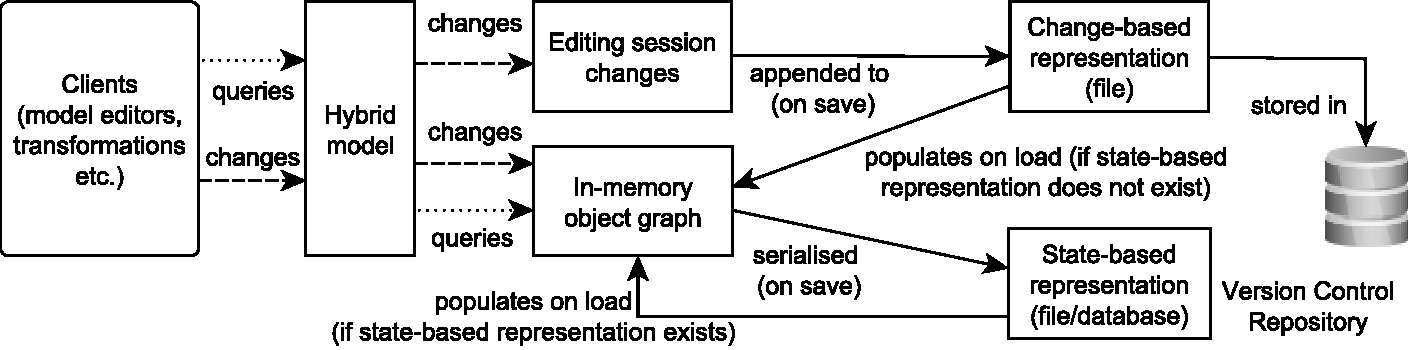
\includegraphics[width=\linewidth]{images/hybrid_persistence}
  \captionof{figure}{The mechanism of hybrid model persistence.}
  \label{fig:hybrid_persistence}
\end{figure}

\textbf{Loading a hybrid model.} Models are loaded into in-memory object graphs that clients (e.g. editors, transformations) can then interact with; depending on the state persistence mechanism, the object graph may be loaded in its entirety at startup (e.g. XMI) or loaded progressively, in a lazy manner (e.g. NeoEMF/CDO \cite{daniel2016neoemf,eclipse2019cdo}). In the proposed hybrid approach, if the state-based counterpart already exists, the in-memory object graph is populated from it; otherwise, it is populated by replaying the complete editing history recorded in the change-based representation.

\textbf{Changing a hybrid model.} When an element in a loaded model is created, modified or deleted, the change is applied to the in-memory object graph and is also recorded in an in-memory list of changes (\textit{Editing session changes} in Fig 2). This work uses the term \emph{editing session} for the period between loading a model and saving back to disk. 

\textbf{Saving a hybrid model.} The current version of the in-memory object graph is stored in the preferred state-based representation. The list of changes recorded in the current editing session (with optional processing, as described above) is appended to the change-based representation.

\textbf{Versioning a hybrid model.} Since the state-based representation is fully derived from the change-based representation, if a model needs to be versioned (e.g. in a Git repository), only the change-based representation needs to be stored. The first time it is loaded after being checked out/cloned, the state-based representation is computed and persisted locally and is used in subsequent model loading steps.

\textbf{Comparing hybrid models.} To compare two hybrid models -- discussed in Chapters \ref{ch:model_differencing} and \ref{ch:conflict_detection}, their change-based representations are used: this is much more efficient than state-based comparison. 

\section{Implementation}
\label{sec:implementation}
This work has implemented the proposed hybrid model persistence approach in a prototype \cite{epsilonlabs2019emfcbp} on top of the Eclipse Modeling Framework (EMF) \cite{steinberg2008emf}. The prototype makes use of an existing implementation of change-based model persistence, the EMF CBP \cite{DBLP:conf/models/YohannisKP17}, augmented with two state-based model persistence implementations: NeoEMF \cite{daniel2016neoemf} and XMI \cite{omg2018xmi}.

\begin{landscape}
\begin{figure}[]
  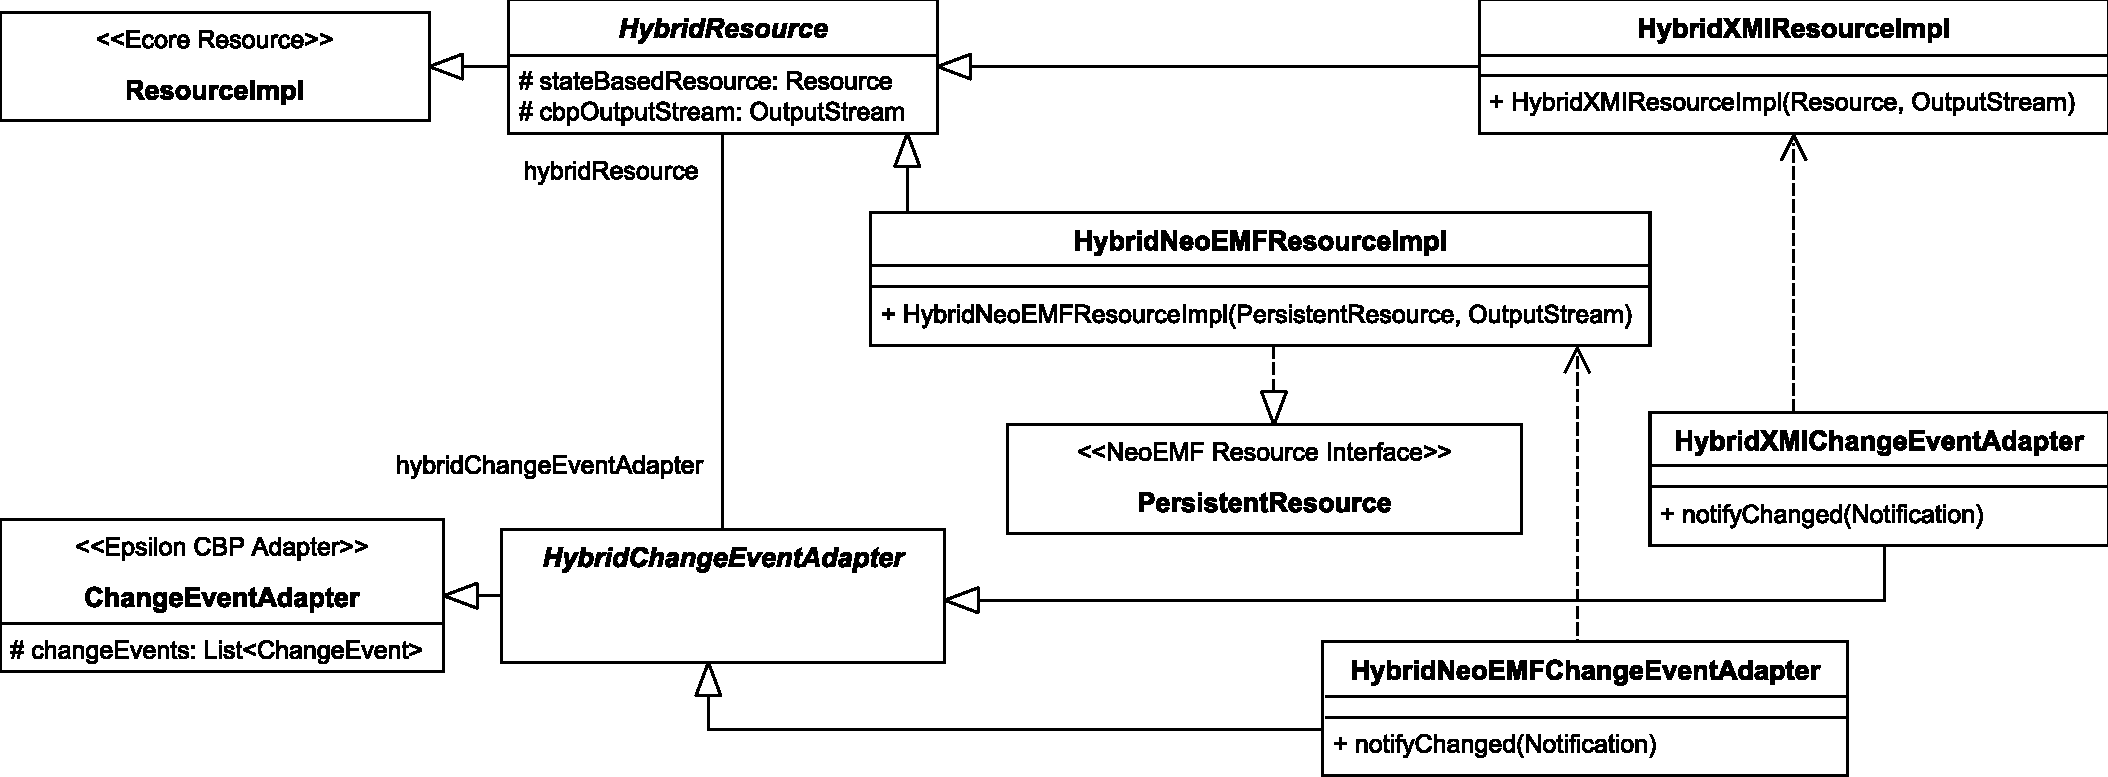
\includegraphics[width=\linewidth]{images/class_diagram}
  \captionof{figure}{Class diagram showing the core components of the hybrid model persistence implementation.}
  \label{fig:class_diagram}
\end{figure}
\end{landscape}

XMI has been selected as a standard state-based model persistence format (natively supported by EMF), and NeoEMF as a best-of-breed representative of database-backed state-based model persistence frameworks. The core components of the prototype are presented in Fig. \ref{fig:class_diagram}. 

The EMF CBP provides a \textsf{ChangeEventAdapter} class \cite{DBLP:conf/models/YohannisKP17} that extends from Ecore's \textsf{EContentAdapter} adapter class \cite{eclipse2018eContentAdapter}
. This class collects changes made to the in-memory object graph of an EMF model in the form of a list of events \textsf{changeEvents}. Based on this class, this work derived an adapter class, \textsf{HybridChangeEventAdapter}, for the hybrid model persistence implementation. It is an abstract class so that it can be further derived to create different implementations of adapter classes for different types of state-based model persistence. The \textsf{HybridNeoEMFChangeEventAdapter} is the adapter class for NeoEMF, and the \textsf{HybridXMIChangeEventAdapter} for XMI. These classes override \textsf{notifyChanged}(\textsf{Notification}) in the \textsf{ChangeEventAdapter} class, to handle events that are specific to NeoEMF and XMI, respectively.

This work also created a resource class for hybrid persistence, \textsf{HybridResource} (a resource class is a class dedicated to interacting with a persistence, e.g. save, load, get contents), derived from the Ecore's \textsf{ResourceImpl} \cite{eclipse2018resourceImpl}
. The class is again abstract so that it can be realised in different resource implementation classes for different state-based model persistence. The \textsf{HybridResource} class contains the \textsf{stateBasedResource} field which is used to refer to a state-based model persistence that is being used, and the \textsf{cbpOutputStream} field that refers to an \textsf{OutputStream} (e.g. file, in-memory) as the representation of the change-based model persistence for saving changes. \textsf{HybridResource} has an association with \textsf{HybridChangeEventAdapater}, so that the former can access the events collected by the latter, and the latter can also use facilities provided by the former (e.g. getting the identity of an element in the resource; saving changes to a change-based model representation).

The resource implementation classes for NeoEMF and XMI are \textsf{HybridNeoEMFResourceImpl} and \textsf{HybridXMIResourceImpl} respectively. \textsf{HybridNeoEMFResourceImpl} also implements the NeoEMF's \textsf{PersistenceResource} interface \cite{atlanmod2018persistentResource}
so that specific NeoEMF's methods can be used (e.g. \textsf{close}(), to close a connection with a backend database).

\section{Evaluation}
\label{sec:evaluation_5}
In this section, this work compares hybrid model persistence (EMF CBP with each of NeoEMF and XMI) vs. state-based model persistence (NeoEMF or XMI only) on storage space usage, loading and saving time and memory footprint, and demonstrate that hybrid model persistence can still perform fast model loading and saving. 

The evaluation was performed on Intel\textsuperscript{\textregistered} Core\textsuperscript{TM} i7-6500U CPU @ 2.50GHz 2.59GHz, 12GB RAM, and the Java\textsuperscript{TM} SE Runtime Environment (build 1.8.0 \textunderscore162-b12). For the evaluation, this work used models reverse-engineered from the Java source code of the Epsilon \cite{eclipse2017epsilon,eclipse2018epsilongit} and BPMN2 \cite{eclipse2017bpmn2} projects. For state-based representation of the models, this work used the MoDisco tool \cite{DBLP:journals/infsof/BruneliereCDM14} to generate XMI-based UML2 \cite{eclipse2017uml2} models that reflect the classes, fields, and operation signatures of the source code of the project and then imported the generated models into NeoEMF. This work also derived MoDiscoXML models \cite{eclipse2018modiscoxml} from the Wikipedia article on the United States \cite{wikipedia2018us}. This work then used reverse-engineering to generate a change-based model persistence for each project based on the differences between consecutive versions of the models.

\begin{table}[ht]
\centering
\begin{footnotesize}
\caption{Space usage for the Epsilon and BPMN2 projects, 
and the Wikipedia's United States article (m = million events, MB = Megabytes, KB = Kilobytes).}
\label{table:space_usage}
\begin{tabular}{| c | c |  c  c c  c  c |}
\hline 
\textbf{Case} & \textbf{\makecell{Generated\\From}} & \textbf{\makecell{Type}} &
\textbf{\makecell{Element\\Count}} & \textbf{\makecell{Event\\Count}} & \textbf{\makecell{Space\\Size}} & \textbf{\makecell{Average\\Space\\Size}}
\\
\hline
%----

\multirow[c]{5}{*}{Epsilon} & \multirow[b]{3}{*}{\makecell{940\\commits}} & XMI & 88,020 & --- &
\makecell{9.44\\MBs} & \makecell{112 bytes/\\element} \\
\hhline{~~-----} 
& & NeoEMF & 88,020 & --- &
\makecell{188\\MBs} & \makecell{2 KBs/\\element} \\
\hhline{~~-----} 
& & \makecell{Epsilon\\CBP} & --- & 4.3 m & \makecell{406\\MBs} & \makecell{98 bytes/\\change event} \\
\hline
%----

\multirow[c]{5}{*}{BPMN2} & \multirow[b]{3}{*}{\makecell{192\\commits}} & XMI & 62,062 & --- & \makecell{6.55\\MBs} & \makecell{110 bytes/\\element} \\
\hhline{~~-----} 
& & NeoEMF & 62,062 & --- &
\makecell{134\\MBs} & \makecell{2 KBs/\\element} \\
\hhline{~~-----} 
& & \makecell{Epsilon\\CBP} & --- & 1.2 m & \makecell{109\\MBs} & \makecell{92 bytes/\\change event} \\
\hline
%----

\multirow[c]{5}{*}{Wikipedia} & \multirow[b]{3}{*}{\makecell{10,187\\versions}} & XMI & 13,112 & --- & \makecell{1.28\\MBs} & \makecell{102 bytes/\\element} \\
\hhline{~~-----} 
& & NeoEMF & 13,112 & --- &
\makecell{31.8\\MBs} & \makecell{2 KBs/\\element} \\
\hhline{~~-----} 
& & \makecell{Epsilon\\CBP} & --- & 62.3 m & \makecell{5.85\\GBs} & \makecell{98 bytes/\\change event} \\
\hline
\end{tabular}
\end{footnotesize}
\end{table}

\subsection{Storage Space Usage}
\label{sec:storage_space_usage}
For the Epsilon project, this work has successfully generated a change-based model persistence from version 1 up to version 940 and also change-based model persistence for the BPMN2 project and Wikipedia article up to version number 192 and 10,187 respectively. The details (element count, event count, space size, and average space size per element or event) of their models, when persisted in XMI, NeoEMF, and EMF CBP are shown in Table \ref{table:space_usage}. The last column of the table derives an average space usage per element (for the state-based model persistence) or event (for the change-based model persistence). Thus, we can estimate the storage space usage for a hybrid model persistence to be the combination of change-based model persistence and the appropriate state-based model persistence space usage.

\subsection{Time and Memory Footprint of Loading and Saving Models}
\label{sec:model_loading_time}
This work evaluated the performance of our hybrid persistence prototype against XMI and NeoEMF regarding time and memory footprint for loading and saving. In the evaluation, experiments were repeated 22 times for each dimension measured. Since the data was not normally distributed, this work used the nonparametric Mann-Whitney U test \cite{doi:10.1002/9780470479216.corpsy0524} with 5\% significance level.

  \begin{table}
    \centering
    \begin{footnotesize}
      \caption{The comparison on time and memory footprint for loading and saving models of the hybrid and state-based-only persistence. The time is in seconds, and the memory footprint is in MBs.}
      \label{table:time_memory_footprint}
      \begin{tabular}{ | c | c | c | c | c | c | c | c | c | }
        \hline
        \multirow{2}{*}{\textbf{\makecell{Dimen\\sion}}} & \multirow{2}{*}{\textbf{Case}} & \multirow{2}{*}{\textbf{Backend}} & \multicolumn{2}{c|}{\textbf{Hybrid}} & \multicolumn{2}{c|}{\textbf{State-based}} & \multicolumn{2}{c|}{\textbf{Significance}} \\
        \hhline{~~~------}
        & & & $mean$ & $sd$ & $mean$ & $sd$ &  $W$ & $p$-$value$ \\
        \hline
        %----------------
        \multirow[c]{6}{*}{\makecell{Loading\\Time}} & \multirow{2}{*}{Epsilon} & NeoEMF & 0.292 & 0.061 & 0.279 & 0.023 & 258 & \textbf{0.72}\\ 
        \hhline{~~-------}
        & & XMI & 0.317 & 0.006 & 0.270 & 0.018 & 26 & $<$ 0.05 \\
        \hhline{~--------}
        &\multirow{2}{*}{BPMN2} & NeoEMF & 0.308 & 0.071 &0.286 & 0.025 & 230 & \textbf{0.79}\\ 
        \hhline{~~-------}
        & & XMI & 0.212 & 0.016 & 0.179 & 0.016 & 37 & $<$ 0.05 \\
        \hhline{~--------}
        &\multirow{2}{*}{Wikipedia}  & NeoEMF & 0.262 & 0.048 & 0.273 & 0.062 & 250 & \textbf{0.86}\\ 
        \hhline{~~-------}
        & & XMI & 0.045 & 0.001 & 0.040 & 0.001 & 0 & $<$ 0.05 \\
        \hline
        \hline
        %--------------------
        
        \multirow[c]{6}{*}{\makecell{Saving\\Time}} & \multirow{2}{*}{Epsilon} & NeoEMF & 0.0892 & 0.0421 & 0.0829 & 0.0494 & 216 & \textbf{0.55}\\ 
        \hhline{~~-------}
        & & XMI & 0.411 & 0.023 & 0.397 & 0.015 & 78 & $<$ 0.05 \\
        \hhline{~--------}
        &\multirow{2}{*}{BPMN2} & NeoEMF & 0.0777 & 0.0424 & 0.0775 & 0.0452 & 213 & \textbf{0.51}\\ 
        \hhline{~~-------}
        & & XMI & 0.33 & 0.007 & 0.28 & 008 & 0 & $<$ 0.05 \\
        \hhline{~--------}
        &\multirow{2}{*}{Wikipedia} & NeoEMF & 0.135 & 0.048 & 0.120 & 0.024 & 218 & \textbf{0.59}\\ 
        \hhline{~~-------}
        & & XMI & 0.024 & 0.048 & 0.020 & 0.002 & 42 & $<$ 0.05 \\
        \hline
        \hline
        %--------------------
        
        \multirow[c]{6}{*}{\makecell{Loading\\Memory\\Footprint}} & \multirow{2}{*}{Epsilon} & NeoEMF & 38.601 & 0.878 & 10.014 & 1.088 & 0 & $<$ 0.05\\ 
        \hhline{~~-------}
        & & XMI & 10.72018 & 0.00022 & 10.72009 & 0.00024 & 0 & $<$ 0.05 \\
        \hhline{~--------}
        &\multirow{2}{*}{BPMN2} & NeoEMF & 40.78 & 1.29 & 27.20 & 1.05 & 0 & $<$ 0.05\\ 
        \hhline{~~-------}
        & & XMI & 6.73367 & 1.29305 & 6.73367 & 0.00056 & 101 & $<$ 0.05 \\
        \hhline{~--------}
        &\multirow{2}{*}{Wikipedia}  & NeoEMF & 35.91 & 1.03 & 27.25 & 0.54 & 27.25 & \textbf{0.54}\\ 
        \hhline{~~-------}
        & & XMI & 8.4079 & 0.0008 & 8.0933 & 0.0009 & 0 & $<$ 0.05 \\
        \hline
        \hline
        %--------------------
        
        \multirow[c]{6}{*}{\makecell{Saving\\Memory\\Footprint}} & \multirow{2}{*}{Epsilon} & NeoEMF & 2.64 & 1.29 & 2.61 & 0.78 & 283 & \textbf{0.34}\\ 
        \hhline{~~-------}
        & & XMI & 1.56355 & 0.0005 & 1.56326 & 0.0018 & 408 & $<$ 0.05 \\
        \hhline{~--------}
        &\multirow{2}{*}{BPMN2} & NeoEMF & 1.86 & 3.86 & 1.52 & 0.77 & 308 & \textbf{0.12}\\ 
        \hhline{~~-------}
        & & XMI & 0.8378 & 0.00361 & 0.8375 & 0.00362 & 58 & $<$ 0.05 \\
        \hhline{~--------}
        &\multirow{2}{*}{Wikipedia}  & NeoEMF & 1.32 & 1.51 & 0.97 & 0.76 & 189 & \textbf{0.22}\\ 
        \hhline{~~-------}
        & & XMI & 0.0010 & 0.00044 & 0.0005 & 0.00001 & 0 & $<$ 0.05\\ 
        \hline
        %--------------------
        
      \end{tabular}
    \end{footnotesize}
  \end{table}

As it can be noticed in Table \ref{table:time_memory_footprint}, all cases experience a slight slowdown on loading and saving time (hybrid approach's $mean$ $>$ state-based approach's $mean$). However, almost for all NeoEMF cases, the slowdown is not significant, which means that the side-effect of the hybrid approach on loading and saving time is still negligible. The hybrid approach also produces a higher memory footprint compared to the state-based-only approach.

\section{Discussion}
\label{sec:discussion_5}
The use of state-based model persistence in hybrid model persistence enables
loading performance that is comparable to the performance of loading only from a state-based persistence, as shown by the result of loading time evaluation in Section \ref{sec:model_loading_time}. In this way, model loading does not have to replay all the changes persisted in its change-based model persistence -- the main challenge for the change-based approach \cite{yohannis2018towards,mens2002state}. Hybrid model persistence performs slightly slower -- statistically significant for Hybrid XMI but insignificant for Hybrid NeoEMF -- compared to loading a state-based model. A slight slowdown also appears on model saving -- statistically significant for Hybrid XMI but insignificant for Hybrid NeoEMF (Section \ref{sec:model_loading_time}). The slowdown is caused by persisting changes into two representations. 

The main drawback of hybrid model persistence is that it consumes more memory when loading and saving and storage space for persisting models compared to state-based representation only (Sections \ref{sec:model_loading_time} and \ref{sec:storage_space_usage}). However, considering the cost of main memory and storage, the trade-off can be acceptable in most real-world scenarios. The summary of the findings can be seen in Table \ref{table:persistence_comparison_conclusion}.

\begin{table}[ht]
  \caption{Hybrid model persistence compared to other persistence approaches.}
  \label{table:persistence_comparison_conclusion}
  \centering
  \begin{small}
    \begin{tabular}{ c c c c }
      \hline 
      \textbf{Dimensions} & \textbf{Change-based} & \textbf{State-based} & \textbf{Hybrid}  \\
      \hline 
      Load Time & $-$ & $+$ & $+$ \\
      Save Time & $+$ & $-$ & $+$ \\
      %      Comparison Time & $+$ & $-$ & $+$ \\
      Storage/Memory & $-$ & $+$ & $-$ \\
      \hline 
    \end{tabular}
  \end{small}
\end{table}

\section{Conclusions}
\label{sec:conclusions_5}
Change-based persistence can be slow when it comes to loading a model since its change records have to be replayed. While in the Chapter \ref{ch:optimised_loading} tried to address by not replaying change events that do not have any effect on eventual states, the performance it gives is not at the level where it outperforms persisting in XMI. This study then implemented a hybrid model persistence -- using change-based and state-based persistence side-by-side -- where models are loaded from its state-based persistence, but changes are saved into both persistence.

This chapter has evaluated hybrid persistence's impact on time and memory footprint for model loading and saving, and storage space usage. Based on the evaluation results, the hybrid model persistence provides benefits on model loading time, since its performance is comparable to loading a model from a change-based persistence only, with trade-offs on increased memory footprint and storage space usage. 

This chapter also has addressed the first research question of this study partially, \textbf{How can models be effectively persisted in a change-based format, and how does change-based persistence perform, compared to state-based persistence on loading and saving models?} (RQ1). Based on the evaluation results, it is best to persist models in hybrid model persistence since it only experiences a slight slowdown, on both loading and saving, compared to persisting models in state-based persistence. In other words, the side-effect of the hybrid approach on loading and saving time is negligible. However, it comes with trade-offs on increased memory footprint and usage of storage space.

\chapter{Efficient Model Differencing of Change-based Models}
\label{ch:model_differencing}


In the previous two chapters, Chapters \ref{ch:optimised_loading} and \ref{ch:hybrid_model_persistence}, this work has proposed two approaches to optimise the loading of change-based model persistence. In this chapter, this research presents a method on how change-based persistence could also be used to identify differences between two versions of a model with much more efficiency in certain circumstances compared to identifying differences in state-based persistence. A detailed discussion on the proposed change-based model differencing and its evaluation are also presented in this chapter.

\section{Introduction}
\label{sec:introduction_06}
In modelling and model management, it is common to find that many versions or variants of a model exist. These versions are commonly persisted as snapshots of the model at a given point in time, in a state-based format such as XMI. Model differencing activities can be applied to the different versions of a model to highlight their differences: changes in properties values, new elements, etc. However, comparing versions of large file-based
%\footnote{Persisting models in databases involves its own challenges which have been discussed extensively in the literature. For the rest of this chapter, we are only concerned with file-based models and we return to database-backed model representations in Section \ref{sec:related_work}.}
models in a state-based format can be computationally expensive since both versions of the model need to be loaded in memory in their entirety before their elements can be matched and diffed. 

In the previous publication part of this research \cite{DBLP:conf/models/YohannisKP17,yohannis2018towards,DBLP:conf/models/YohannisRPK18}, this work proposed change-based model persistence (CBMP) as an alternative approach to state-based model persistence of EMF models \cite{steinberg2008emf}. Instead of persisting models as XMI snapshots, in the proposed approach models are persisted as a complete history of changes. We demonstrated the substantial performance benefits of change-based model persistence in terms of saving changes to large models \cite{DBLP:conf/models/YohannisKP17} as well as the method for reducing model loading time compared to naively replaying all recorded change events \cite{DBLP:conf/models/YohannisRPK18} to reconstruct the state of a change-based model. 
This chapter demonstrates how a change-based representation also enables much more efficient and performant model differencing between versions of the same model. Our experiments, presented in Section \ref{sec:evaluation_6}, demonstrate savings of the order of 90\% for (relatively) small changes made to large models.

This chapter is structured as follows. Section \ref{sec:state-based_model_differencing} presents the state-based model differencing performed in EMF Compare \cite{emfcompare2018developer}. 
Section \ref{sec:change_based_approach_for_comparing_models} presents our change-based approach to speed up model differencing and its implementation. 
Section \ref{sec:evaluation_6} reports on the results of evaluation experiments used to evaluate the proposed approach.

\section{State-based Model Differencing}
\label{sec:state-based_model_differencing}
Referring to the example in Section \ref{sec:running_example_1}, at one time, Bob decides to compare his model to Alice's model because he is interested to analyse the differences between their models. Bob then uses a model differencing tool and perform state-based model differencing. 
In state-based model differencing, comparing models commonly consists of two steps: \emph{matching} and \emph{diffing}.
The matching process establishes matches between the elements of both models, to determine the elements in the left model that correspond to elements in the right model. Generally, the matching process iterates through all the elements of the models being compared and matches them by their identifiers or through a similarity mechanism  \cite{DBLP:conf/sfm/BroschKLSWW12,emfcompare2018developer}. The diffing process then identifies differences between the matched elements \cite{DBLP:conf/sfm/BroschKLSWW12,emfcompare2018developer}. 

In our example, the matching process in state-based comparison -- as performed by EMF Compare \cite{emfcompare2018developer} -- iterates through all the elements of both models and matches them using their identifiers. The matching process yields 10 matches: $m_1$ = (\textsf{character}, \textsf{character}), $m_2$ = (\textsf{attack}, \textsf{attack}), $m_3$ = (\textsf{gem}, \textsf{gem}), $m_4$ = (\textsf{weapon}, \textsf{weapon}), $m_5$ = (\textsf{target}, \textsf{target}), $m_6$ = (\textsf{troll}, \textsf{troll}), $m_7$ = (\textsf{knight}, \textsf{knight}), $m_8$ = (\textsf{smash}, \textsf{smash}), and $m_9$ = (\textsf{mage}, \textsf{mage}), and 3 unmatched elements, $um_1$ = (-, \textsf{giant}), $um_2$ = (-, \textsf{rightGen}), $m_3$ = (-, \textsf{cast}), and $um_4$ = (\textsf{leftGen}, -). 

The diffing process then iterates through all the matches and unmatched elements and uses an LCS algorithm to identify their differences. During iterating the matches, in the second match $m_2$, it identifies that, in order to make the left feature \textsf{parameters} equal to the right feature \textsf{parameters}, parameter \textsf{gem} has to be moved from index 1 to 0 (diff $ds_1$). It is important to note that the employed LCS algorithm does not detect the different position of parameter \textsf{weapon}; it only identifies the minimum number of differences which if all are resolved unidirectionally can make both models equal. Otherwise, the number becomes less optimal -- not minimum.

In the six match $m_6$, The diffing process identifies that the classes \textsf{troll} are different in their \textsf{name}. The left \textsf{troll}'s \textsf{name} is ``Ogre'' while the other \textsf{troll}'s \textsf{name} is ``Orc'' (diff $ds_2$). In the eight match $m_8$, the diffing process identifies that the containers of operation \textsf{smash} are different. Thus, element \textsf{smash} has to be move from \textsf{knight}'s \textsf{operations} to \textsf{giant}'s \textsf{operations} (diff $ds_3$). For the other matches, the diffing process does not identify any differences. 

From the unmatched elements ($um_1$, $um_2$, $um_3$, and $um_4$), the diffing process identifies that, in order to make the left model equal to the right model, class \textsf{giant} has to be added to the left model's resource at index 2 (diff $ds_4$), generalization \textsf{rightGen} has to be added to class \textsf{mage}' s \textsf{generalization} (diff $ds_5$), operation \textsf{cast} has to be added to class \textsf{mage}'s \textsf{operations} (diff $ds_6$), and  generalization \textsf{leftGen} has to be removed from class \textsf{knight}' s \textsf{generalization} (diff $ds_7$).

Differences are commonly expressed as a list of changes that must be applied to a target model so that it is made equal to a reference model. This work treats the left model as a reference model and the right model as the target model. This means that differences are expressed as changes applied to the right model so that it equals the left model. To express differences, this work uses the following terms: \textsf{LeftContainer}, \textsf{RightContainer}, \textsf{LeftFeature}, \textsf{RightFeature}, \textsf{LeftIndex}, \textsf{RightIndex}, \textsf{LeftValue}, \textsf{RightValue}, and \textsf{Kind}. The \textsf{*Container}, \textsf{*Feature}, and \textsf{*Value} are the target element, feature, and value involved in a difference (\textsf{*} symbol can be replaced with \textsf{Left} and \textsf{Right}). \textsf{*Index} is the index of a value in a feature. \textsf{Kind} is the type of difference. It can be one of these types: \textsf{CHANGE}, \textsf{ADD}, \textsf{DELETE}, and \textsf{MOVE}. \textsf{CHANGE} means a pair of single-valued features have different values. \textsf{ADD} indicates that a value does not exist in the right model, thus it requires the addition of the value. \textsf{DELETE} is the opposite of \textsf{ADD}. \textsf{MOVE} indicates that matched elements differ in terms of their containers, containing features, or indexes. A Container is an element that contains a value. A containing feature is a feature owned by a container in which a value is contained. An index is the position of a value in a containing feature.

Based on these definitions, this work can express the result of the diffing process as: $ds_{n}$ = [$LeftContainer_n$, $RightContainer_n$, $LeftFeature_n$, $RightFeature_n$, $LeftIndex_n$, $RightIndex_n$, $LeftValue_n$, $RightValue_n$, $Kind_n$]. Therefore:

$ds_{1}$ =  [\textsf{attack}, \textsf{attack}, \textsf{parameters}, \textsf{parameters}, 0, 1, \textsf{gem}, \textsf{gem}, \textsf{MOVE}]\\
$ds_{2}$ = [\textsf{troll}, \textsf{troll}, \textsf{name}, \textsf{name}, 0, 0, ``Ogre'', ``Orc'', \textsf{CHANGE}]\\
$ds_{3}$ = [\textsf{knight}, \textsf{giant}, \textsf{operations}, \textsf{operations}, 0, 0, \textsf{smash}, \textsf{smash}, \textsf{MOVE}]\\
$ds_{4}$ = [\textsf{resource}, \textsf{resource}, \textsf{null}, \textsf{null}, \textsf{null}, \textsf{null}, \textsf{null}, \textsf{giant}, \textsf{DELETE}]\\
$ds_{5}$ = [\textsf{mage}, \textsf{mage}, \textsf{generalization}, \textsf{generalization}, \textsf{null}, 0, \textsf{null}, \textsf{rightGen}, \textsf{DELETE}] \\
$ds_{6}$ = [\textsf{mage}, \textsf{mage}, \textsf{operations}, \textsf{operations}, \textsf{null}, 0, \textsf{null}, \textsf{cast}, \textsf{DELETE}]\\
$ds_{7}$ = [\textsf{knight}, \textsf{knight}, \textsf{generalization}, \textsf{generalization}, 0, \textsf{null}, \textsf{leftGen}, \textsf{null}, \textsf{ADD}]

This work then can use this information to represent the diffs visually as depicted in Figure \ref{fig:xmi_comparison}. We can also transform these diffs into change events that if the diffs are executed as changes to the right model, they transform it into the left model and generate relevant change events. The change events are presented in Listing \ref{lst:readable_diffs}. Diff $ds_{1}$ produces the change event at line 1 in Listing \ref{lst:readable_diffs}, $ds_{2}$ produces line 2, $ds_{3}$ produces lines 3-4, $ds_{4}$ produces lines 5-7, $ds_{5}$ produces lines 8-10, $ds_{6}$ produces lines 11-13, and $ds_{7}$ produces lines 14-16.

\begin{figure}[ht]
  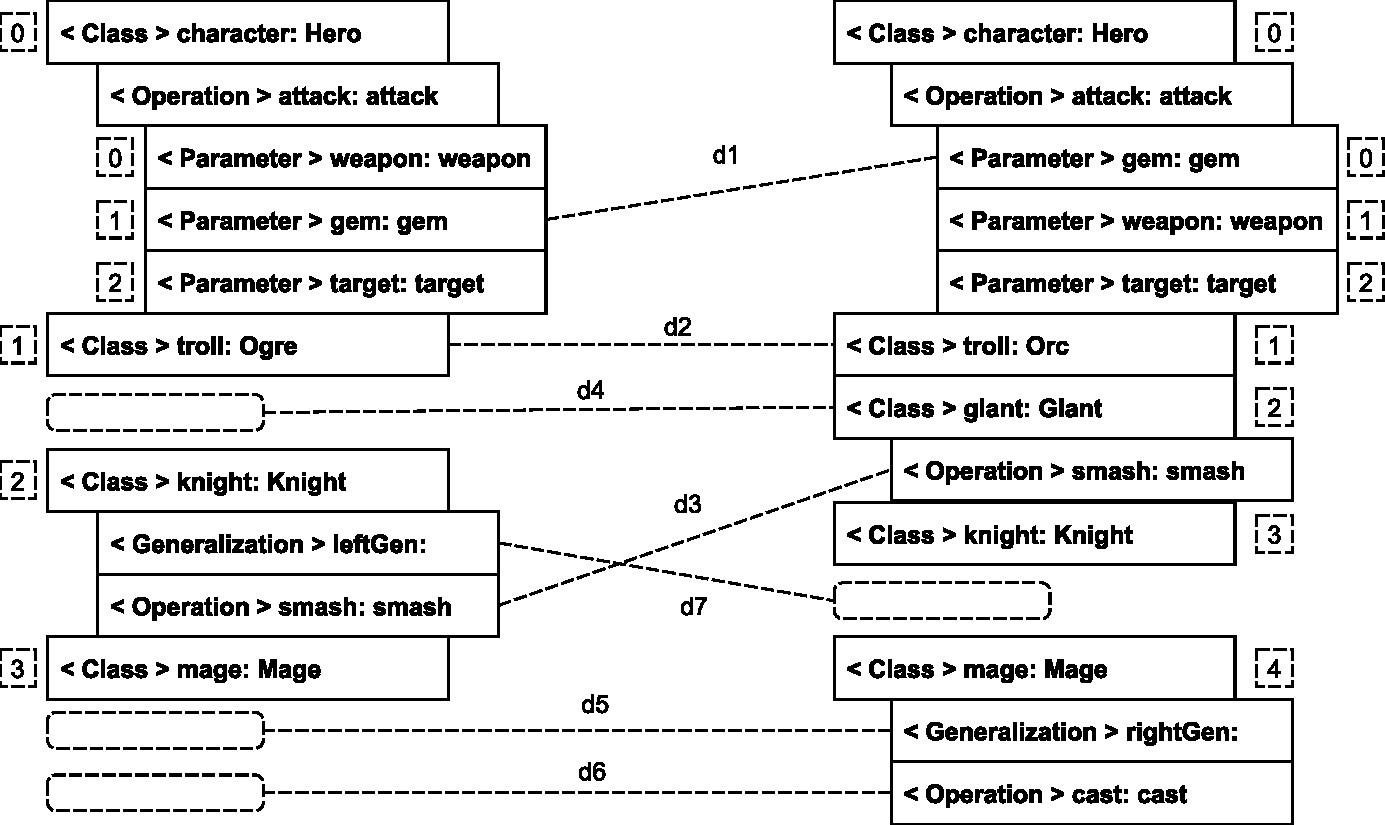
\includegraphics[width=\linewidth]{XmiComparison}
  \caption{A model comparison of the left and right models in Listings \ref{lst:xmimodel_left} and \ref{lst:xmimodel_right}.}
  \label{fig:xmi_comparison}
\end{figure}

\vspace{-20pt}
\begin{lstlisting}[firstnumber=1,style=eol,caption={The identified diffs presented as change events.},label=lst:readable_diffs]
move gem in attack.parameters from 0 to 1
set troll.name from "Orc" to "Ogre"
remove smash from giant.operations at 0 composite c1
add smash to knight.operations at 0 composite c1
unset giant.name from "Giant" to null composite c2
remove giant from resource at 2 composite c2
delete giant composite c2
unset mage.generalization from rightGen to null composite c3
unset rightGen.general from character to null  composite c3
delete rightGen composite c3
unset cast.name from "cast" to null composite c4
remove cast from mage.operations composite c4
delete cast composite c4
create leftGen type Generalization composite c5
set knight.generalization from null to leftGen composite c5
set leftGen.general from null to character composite c5
\end{lstlisting}

\section{Change-based Model Differencing}
\label{sec:change_based_approach_for_comparing_models}
Compared to the state-based model conflict detection of EMF Compare, the change-based model conflict detection proposed in this work consists of three phases: event loading, element tree construction, and conflict computation.
The conflict detection is not performed over all the elements of the model as opposed to state-based model differencing; instead, the approach only needs to compare the last sets of change events of the two models being compared, starting from the lines of both models are different. A simplified class diagram of the approach's implementation \cite{epsilonlabs2019emfcbp} is depicted in Figure \ref{fig:approach_class_diagram}. The three phases are described in detail in the following Sections.

\subsection{Event Loading}
\label{sec:event_loading}
In the event loading phase, the implementation loads change events recorded in two change-based model persistence files into memory.
The most important aspect of this phase is the partial loading as only lines starting from the position where the two files are different are loaded.
Thus, not the whole model needs to be traversed and loaded.
In this case, lines 1-29 in Listing \ref{lst:cbp_origin} are skipped. Only lines starting from line 30 in Listings \ref{lst:cbp_left} and \ref{lst:cbp_right} are loaded, yielding two partial -- left and right -- change-event models. 

\subsection{Element Tree}
\label{sec:tree_construction}
An element tree is a representation of the changes of model elements in the source and reference models. It contains detailed information about elements and their properties. It contains similar information to that captured in change lists in state-based model persistence, but also provides more information about the changes. For example, the element tree can keep track of a feature's old value and element/value's indexes inside multi-valued properties. The element tree only contains the partial states of affected elements of the original, left, and right models as depicted in Figures \ref{fig:left_element_tree_diagram} and \ref{fig:right_element_tree_diagram}.

To better understand the construction of an element tree from change events, we use the following running example using both change events in the Listings \ref{lst:cbp_left} and \ref{lst:cbp_right}. We start from the left change events. 

\begin{landscape}
  \begin{figure}
    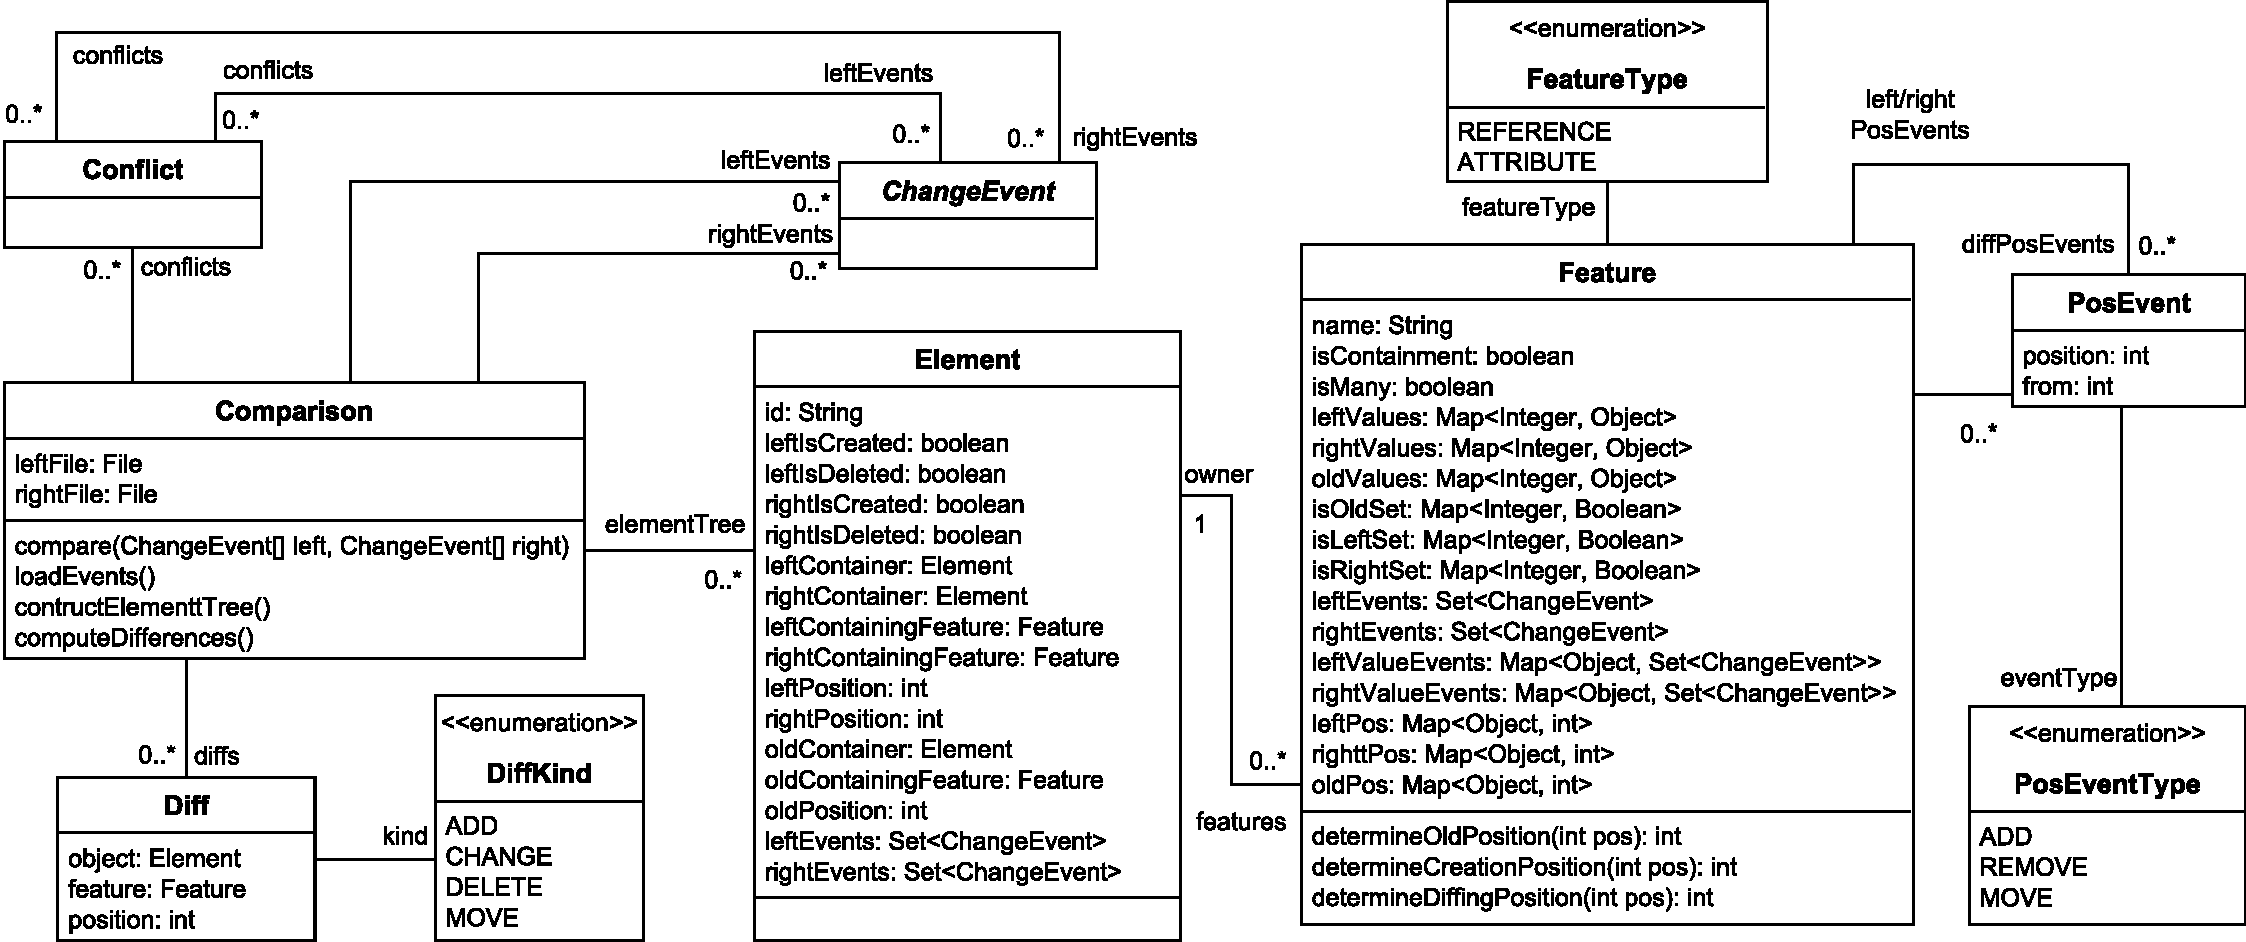
\includegraphics[width=\linewidth]{TreeClassDiagram}
    \caption{A class diagram showing the core components of the change-based approach to speed up model differencing and conflict detection.}
    \label{fig:approach_class_diagram}
  \end{figure}
\end{landscape}

\subsubsection{Left Side}\label{sec:left_side}
In the first change event in Listing \ref{lst:cbp_left} at line \ref{line:cbp_left_30}, the change event is a \textsf{session} event. It marks that the all the following change events until the final line or next \textsf{session} event are persisted in one batch when saving. At line \ref{line:cbp_left_31}, we can identify that Bob created a \textsf{Generalization} with id \textsf{leftGen}. Thus, in \textsf{elementTree}, an element with id \textsf{leftGen} is also created. To mark that an element is newly created in the session, we put a '+' sign at the left lower box of element \textsf{leftGen} in Figure \ref{fig:left_element_tree_diagram}.

\begin{figure}[ht]
  \centering
  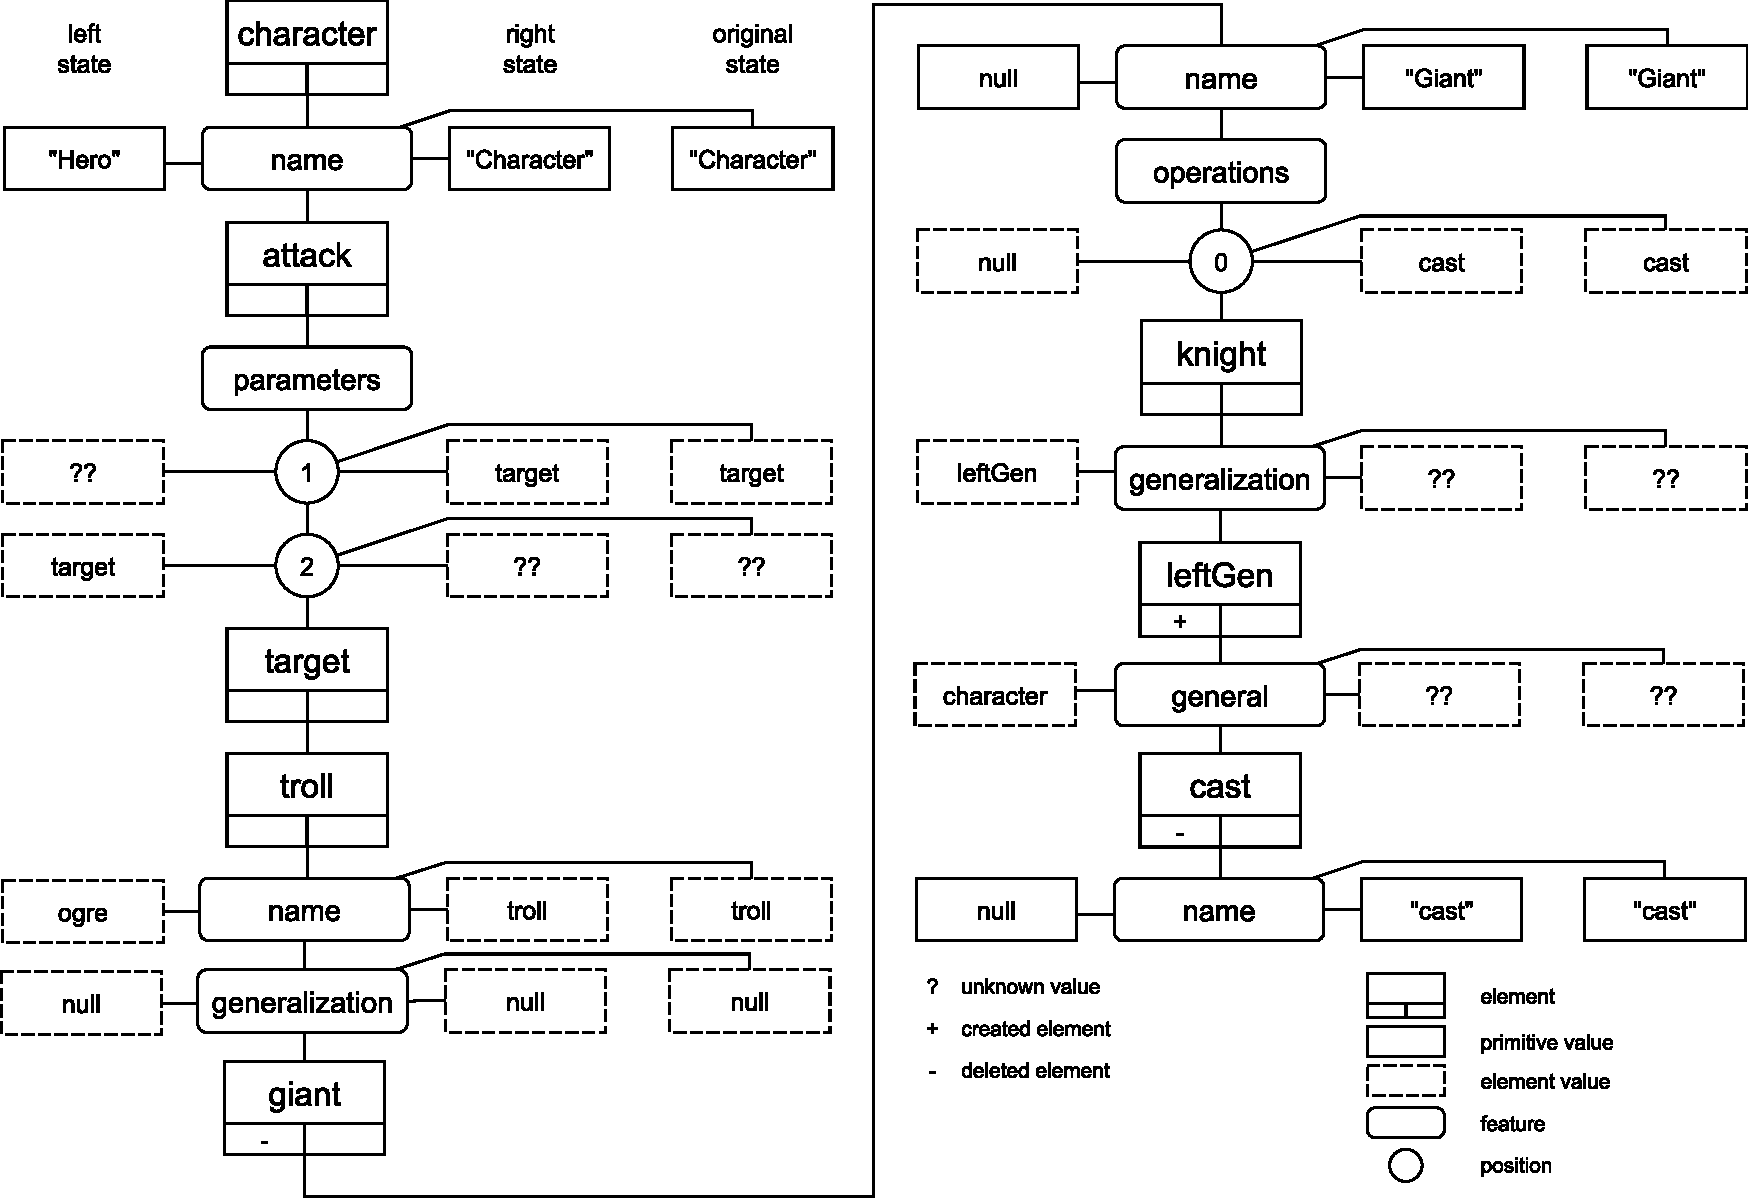
\includegraphics[width=\linewidth]{element_tree_game_left}
  \caption{An element tree constructed using information contained in CBPs in Listing \ref{lst:cbp_left} (all left change events only).}
  \label{fig:left_element_tree_diagram}
\end{figure} 

At line \ref{line:cbp_left_32}, the feature \textsf{general} of \textsf{leftGen} is set to \textsf{character}. From the change event, we can recognise that \textsf{character} has been existed since the previous version since it has never been created in the current editing session. Thus, we create an element with id \textsf{character} as well as the feature \textsf{general} of \textsf{leftGen} and put them in \textsf{elementTree} and then set the value of \textsf{general} to \textsf{character} on the left side. We also do the same routine to \textsf{troll} and \textsf{generalization} at line \ref{line:cbp_left_33}, adding element \textsf{troll} and feature \textsf{generalization} to \textsf{elementTree} and set the value of feature \textsf{generalization} to \textsf{leftGen} on the left side of the \textsf{elementTree}. 

Change event at line \ref{line:cbp_left_34}, change \textsf{character}'s \textsf{name} from ``Character'' to ``Hero''. From the change event, we can identify that \textsf{character} has been existed before. Thus, we create element \textsf{character} and feature \textsf{name} into \textsf{elementTree}. We also set the value of \textsf{name} to ``Hero'' on the left side. Since this set change event is the first event for \textsf{character}'s \textsf{name}, we can infer that original value of \textsf{name} is ``Character''. Thus, we set \textsf{name}'s value to ``Character'' on the original side. The value of \textsf{name} on the right side is also set to ``Character'' but will be modified later once we process the right change events (Alice's change events) if there is any change event that affects it. The same routine is also applied when we process the change event at line \ref{line:cbp_left_43} later.

Lines \ref{line:cbp_left_35} and \ref{line:cbp_left_36} are the changes events of  composite move event \textsf{l1}. Element \textsf{leftGen} is removed (unset) from \textsf{troll}'s \textsf{generalization} and then is assigned (set) to \textsf{knight}'s \textsf{generalization}. From these change events, we can identify that element \textsf{knight} also already existed since the original version. Thus, we add it into \textsf{elementTree} together with its  \textsf{generalization} feature. Element \textsf{troll} and its  \textsf{generalization} feature are not added into \textsf{elementTree} any more since they were already added when processing line \ref{line:cbp_left_33}. In \textsf{elementTree}, we set \textsf{troll}'s \textsf{generalization} to null since element \textsf{leftGen} is moved to \textsf{knight}'s \textsf{generalization}.

At line \ref{line:cbp_left_37}, \textsf{target} is moved from index 1 to 2 in \textsf{attack}'s \textsf{parameters}. From the change event, we can identify that there has been element \textsf{target} contained in \textsf{attack}'s \textsf{parameters} at index 1 since the original version. Thus, we put element \textsf{target} and element \textsf{attack} and its \textsf{parameters} feature into \textsf{elementTree}. We also create a map on the left side with a key `2' and a value that points to element \textsf{target} for feature \textsf{parameters}, indicating \textsf{target} is at index 2 in the left version. Since it is the first change event that moves \textsf{target}, we can decide that \textsf{target} is at index 1 in the original version. Thus, we create another map on the original side a map on the left side with a key `1' and a value that also points to \textsf{target}. We also perform this routine to the right side of feature \textsf{parameters}, creating a map with a key `1' and a value that also points to \textsf{target}. It will be modified later once we process the right change events (Alice's change events) if there is any change event that affects the index of \textsf{target}.

Lines \ref{line:cbp_left_38} to \ref{line:cbp_left_42} are the change events of  composite delete event \textsf{l2}; a deletion of element \textsf{giant}. 
A deletion of an element unsets all the features of the elements and its sub elements, removes the sub elements from their containers, and deletes the sub elements and the element from the model. 
As can be noticed,  at line \ref{line:cbp_left_38}, the value of \textsf{cast}'s \textsf{name}  is unset from ``cast'' to null. From the change event, we know that cast has been existed since the original version. Thus, we add element \textsf{cast} and its feature \textsf{name} to \textsf{elementTree} and set its value null on the left side and ``cast'' on the origin and right sides. 

At line \ref{line:cbp_left_39}, \textsf{cast} is removed from \textsf{giant}'s \textsf{operations} at index 0. From it, we can identify that \textsf{giant} and its feature \textsf{operations} exists, and \textsf{cast} is contained in \textsf{giant}'s \textsf{operations} at index 0 in the original version. Thus, we create element \textsf{giant} and its feature \textsf{operations} in \textsf{elementTree}. Three maps also are created in \textsf{operations} for the three sides. Each map contains a key `0', indicating index, and a value that points to element \textsf{cast} except on the left side the value is null since \textsf{cast} is removed from \textsf{giant}'s \textsf{operations}. The deletion of \textsf{cast} at line \ref{line:cbp_left_40} marks \textsf{cast} in \textsf{elementTree} with `-' sign on the left side indicating that the element is deleted from the model in the left version.

Change event at line \ref{line:cbp_left_41} is similar to change event at line At line \ref{line:cbp_left_38} except that it is applied to \textsf{giant}'s \textsf{name}. Since \textsf{giant} has existed in \textsf{elementTree}, only the feature \textsf{name} is added. Its value is set to null on the left side and ``Giant'' on the origin and right sides. The deletion of \textsf{giant} at line \ref{line:cbp_left_42} marks \textsf{giant} in \textsf{elementTree} with `-' sign indicating that the element is deleted from the model in the left version.

Figure \ref{fig:left_element_tree_diagram} illustrates the state of the \textsf{elementTree} after all left change events have been processed. As can be seen, the \textsf{elementTree} exhibits the partial states of the original, left, and right models at once. 

\subsubsection{Right Side}\label{sec:right_side}
In Listing \ref{lst:cbp_right}, similar to processing the left change events, the processing of the right change events (Alice's version) starts with processing the session event at line \ref{line:cbp_right_30}. At line \ref{line:cbp_right_31}, \textsf{target} is moved from index 1 to 0 in \textsf{attack}'s \textsf{parameters}. Since the index of \textsf{target} is already determined when processing the change event, we only determine the index of \textsf{target} on the right side. We unset the value of key `1' on the right side to null and create a new key `0' that maps its value to \textsf{target}.

Composite move event \textsf{r1} at lines \ref{line:cbp_right_32} and \ref{line:cbp_right_33} moves \textsf{smash} from \textsf{knight}'s \textsf{operations} to \textsf{giant}'s \textsf{operations}. From this move event, we can identify \textsf{smash} is no longer in \textsf{knight}'s \textsf{operations} but contained in \textsf{giant}'s \textsf{operations} on the right side. Element \textsf{smash} has never existed in \textsf{elementTree}. So, we create and add \textsf{smash} to \textsf{knight}'s \textsf{operations} at index 0 on the origin side and to \textsf{giant}'s \textsf{operations} at index 0 on the right side. Since \textsf{smash} is not modified on the left side and no other change events applied to \textsf{knight}'s \textsf{operations}, we can determine that \textsf{smash} is at index 0 in \textsf{giant}'s \textsf{operations} on the left side.

Lines \ref{line:cbp_right_34} to \ref{line:cbp_right_35} are change events that constitute composite move event \textsf{r2}.  It  moves \textsf{cast} from \textsf{giant}'s \textsf{operations} to \textsf{mage}'s \textsf{operations}. From this move event, we can identify \textsf{cast} is no longer in  \textsf{giant}'s \textsf{operations} but now exists in \textsf{mage}'s \textsf{operations} on the right side. Element \textsf{mage} and its feature \textsf{operations} have never existed in \textsf{elementTree}. So, we create and add them to \textsf{elementTree} and add \textsf{cast} to \textsf{mage}'s \textsf{operations} on the right side.

At line \ref{line:cbp_right_36}, we can identify that Alice created a \textsf{Generalization} with id \textsf{rightGen}. Thus, in \textsf{elementTree}, an element with id \textsf{rightGen} is also created. Since it has just been created in the active session, the element is marked with '+' sign in \textsf{elementTree} on the right side. At line \ref{line:cbp_right_37}, we can also identify that feature \textsf{general} should be added to \textsf{rightGen} in \textsf{elementTree} and the value is set to \textsf{character} on the right side. We also set \textsf{mage}'s \textsf{operations} to \textsf{rightGen} on the right side of  \textsf{elementTree} according to the change event at line \ref{line:cbp_right_38}. 

Change event at line \ref{line:cbp_right_39}, change \textsf{character}'s \textsf{name} from ``Character'' to ``Hero''. Since \textsf{character} and its feature \textsf{name} already exists in \textsf{elementTree}, we only set \textsf{name}'s value to ``Hero'' on the right side; the original value has already been assigned when processing left change events. We apply the same routine when processing the change event at line \ref{line:cbp_right_42} later.

\begin{figure}[ht]
  \centering
  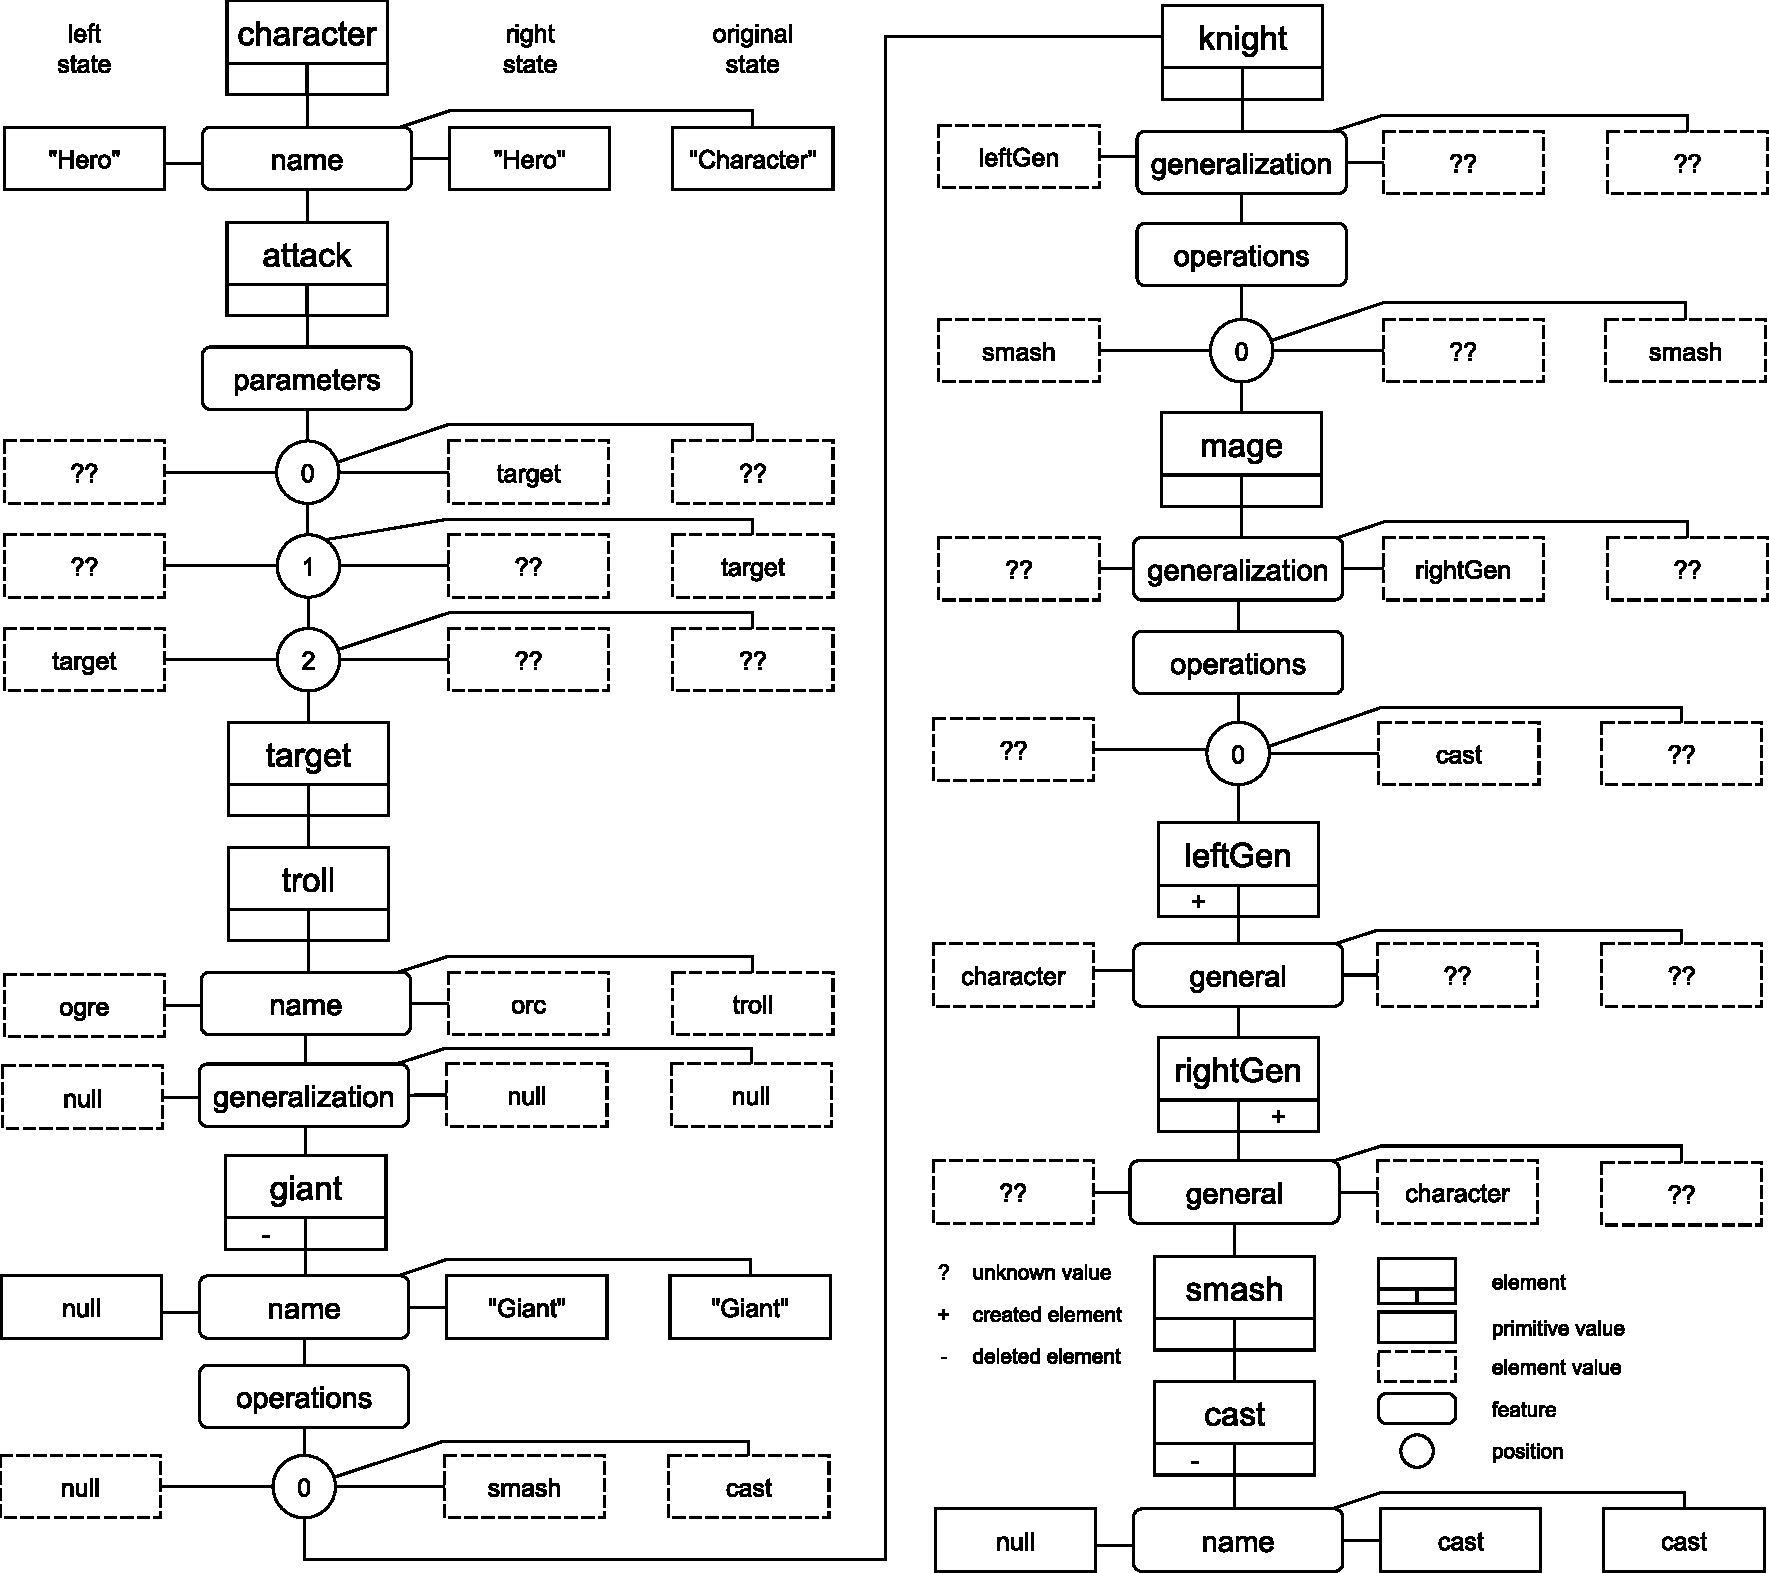
\includegraphics[width=\linewidth]{element_tree_game_right}
  \caption{An element tree constructed using information contained in CBPs in Listings \ref{lst:cbp_left} and \ref{lst:cbp_right} (all left and right change events).}
  \label{fig:right_element_tree_diagram}
\end{figure} 

Composite move event \textsf{r3} at lines \ref{line:cbp_right_40} and \ref{line:cbp_right_41} moves \textsf{rightGen} from \textsf{troll}'s \textsf{generalization} to \textsf{mage}'s \textsf{generalization}. From this move event, on the right side, we can identify \textsf{rightGen} is no longer in \textsf{troll}'s \textsf{generalization} but exists in \textsf{mage}'s \textsf{generalization}. Since it's the first \textsf{mage}'s \textsf{generalization} is modified, we create and add the feature to \textsf{mage} in \textsf{elementTree}. On the right side of \textsf{elementTree}, we unset \textsf{troll}'s \textsf{generalization} to null and assign \textsf{rightGen} to \textsf{mage}'s \textsf{generalization}.

Figure \ref{fig:right_element_tree_diagram} exhibits the state of the \textsf{elementTree} after both sides' change events have been processed.

\begin{figure}
    \centering
    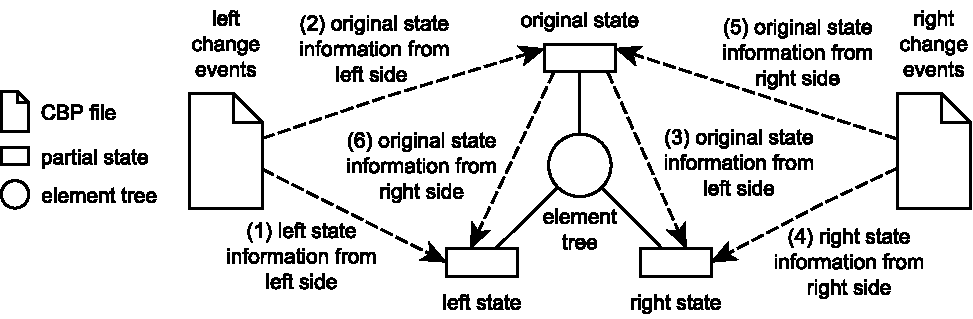
\includegraphics[width=\linewidth]{TreeConstruction}
    \caption{Steps in Element Tree construction.}
    \label{fig:tree_construction}
\end{figure} 

\subsubsection{Construction Procedure}\label{sec:construction_procedure}
The construction of \textsf{elementTree} that has been explained follows the steps shown in Figure \ref{fig:tree_construction}. First, the partial
state $S_{L}$ of the left model in the \textsf{elementTree} is constructed based on the information retrieved from the left change events (step 1). We denote this information as $I_{LL}$. We can also construct the partial 
state $S_{O}$ of the original model using the information related to the original state contained in the left change events $I_{OL}$ (step 2). The information $I_{OL}$ allows us to construct the initial partial 
state $S_{R}$ of the right model 
(step 3). Similarly, using the information from the right change events $I_{RR}$, we update the partial right state $S_{R}$ that has been initialised before using the information $I_{OL}$ (step 4), implying that $I_{OL} \cup I_{RR} \rightarrow S_{R}$. Also, information related to the state of the original model from the right change events $I_{OR}$ is used to update the original state  (step 5). Thus, we have a partial state of the original model constructed using information from both left and right sides, $I_{OL} \cup I_{OR} \rightarrow S_{O}$. Finally, we also use the information $I_{OR}$ to update the partial state of the left model (step 6), implying that $I_{LL} \cup I_{OR} \rightarrow S_{L}$.  

Algorithm \ref{alg:element_tree} describes the steps presented in Figure \ref{fig:tree_construction} in a generic fashion. It iterates through all of a model's change events and uses the information contained in them to construct the relevant partial state. The selection of side, left or right change events, that are executed first depends on the \textsf{Side} enumeration value -- \textsf{left} or \textsf{right} -- passed through the parameter \textsf{side} (the second input parameter). In our implementation, we process the left side first by default. The algorithm also receives an input of the change events \textsf{events} that are to be iterated and the element tree \textsf{elementTree} that has been instantiated before, and then returns the \textsf{elementTree} as output after updating it.

For each \textsf{event} in the \textsf{events}, we collect information needed to build up \textsf{elementTree}  (lines 3-9), such as \textsf{targetElement}, \textsf{feature}, \textsf{value}, \textsf{previousValue}, \textsf{index}, and \textsf{previousIndex}. The \textsf{targetElement} is the element modified by a change event (e.g., \textsf{character} and \textsf{giant} in Listing \ref{lst:cbp_left}). This \textsf{targetElement} -- an instance of class Element in Figure \ref{fig:approach_class_diagram} -- is retrieved from the \textsf{elementTree} if it already exists. Otherwise, a new element is created and added to the \textsf{elementTree} (line 3). In this step we also set the flags \textsf{*IsCreated} and \textsf{*IsDeleted} of the element in Figure \ref{fig:approach_class_diagram}. For example, if the type of the event is \textsf{create} then \textsf{*IsCreated} is set to \textsf{true}. The \textsf{feature} -- an instance of class Feature in Figure \ref{fig:approach_class_diagram} -- represents the target element's feature (e.g., \textsf{name} and \textsf{operations} in Listing \ref{lst:cbp_right}) modified by a change event. It is retrieved from the \textsf{targetElement}'s feature list, and a new one is created and added to the \textsf{targetElement}'s feature list if the feature does exist (line 5). 

\IncMargin{1.5em}
\begin{algorithm}[H]
    \begin{footnotesize}
        \SetKwInOut{Input}{input} 
        \SetKwInOut{Output}{output}
        \Input{a list of ChangeEvent $events$}
        \Input{an enumeration of Side $side$}
        \Input{an instance of ElementTree $elementTree$}
        \Output{an instance of ElementTree $elementTree$}
        \SetKwBlock{Beginn}{beginn}{ende}
        \Begin{
            \ForEach{$event$ in $events$}{
                $targetElement$ $\leftarrow$ getOrCreateNewTargetElement($event$, $elementTree$)\;
                $feature$ $\leftarrow$ getOrCreateNewFeature($event$, $targetElement$)\;
                $value$ $\leftarrow$ getValue($event$)\;
                $previousValue$ $\leftarrow$ getPreviousValue($event$)\;
                $index$ $\leftarrow$ getIndex($event$)\;
                $previousIndex$ $\leftarrow$ getPreviousIndex($event$)\;
                $featureEventList$ $\leftarrow$ getFeatureEventList($feature$, $side$)\;
                
                \BlankLine
                \tcp{put all values to their proper indexes}
                updateTree($targetElement$, $feature$, $value$, $index$, $side$)\;
                $oldIndexes$ $\leftarrow$ calculateOldIndex($featureEventList$, $previousIndex$, $side$)\;
                \If{\Not isCreated($value$, $side$) \AndA \Not isOldValueSet($feature$, $previousValue$, $previousIndex$, $side$)} {
                    setOldValue($feature$, $previousValue$, $oldIndex$, $side$)\;
                    $oppositeFeatureEventList$ $\leftarrow$ getOppositeFeatureEventList($feature$, $side$)\;
                    $oppositeIndex$ $\leftarrow$ calculateOppositeIndex($oppositeFeatureEventList$, $oldIndex$, $side$)\;
                    \If{\Not isDeleted($value$, $side$) \AndA \Not isOppositeSideValueSet($feature$, $value$, $oppositeIndex$, $side$)} {
                        setOppositeSideValue($feature$, $value$, $oppositeIndex$, $side$)\;
                    }
                }   
                
                addEventToFeatureEventList($event$, $featureEventList$)\;
                
            }
            \Return{$elementTree$}\;
        }
    \end{footnotesize}
    \caption{Algorithm to construct an element tree from events.}
    \label{alg:element_tree}
\end{algorithm}
\DecMargin{1.5em}

The \textsf{value} is the value assigned to the feature in a change event (line 5, Algorithm \ref{alg:element_tree}). The \textsf{value} can be the type of \textsf{Element} (e.g., element \textsf{leftGen} line \ref{line:cbp_left_36} in Listing \ref{lst:cbp_left}) or primitive (e.g., the string ``Hero'' at line \ref{line:cbp_left_34} in the Listing \ref{lst:cbp_left}). The \textsf{previousValue} represents the previous value of the modified feature (line 6, Algorithm \ref{alg:element_tree}). The \textsf{previousValue} is not defined if no previous value has been assigned. For \textsf{value} and \textsf{previousValue} with type \textsf{Element}, the elements that they represent are retrieved from the \textsf{elementTree}, and if they do not exist, new instances are created. If the type is primitive, the value is treated as it is. Not every change event has a \textsf{value}, particularly events with type \textsf{create} 
or \textsf{delete} which only modify a target element not the element's feature.

The \textsf{index} is the index assigned by a change event to a value in a feature, while \textsf{previousIndex} is the previous index of the value (lines 7-8, Algorithm \ref{alg:element_tree}). In one change event, we can get both \textsf{index} and \textsf{previousIndex} or only one of them depending on the type of the change event. For example, we can obtain that the \textsf{index} of \textsf{cast} is 0 (line \ref{line:cbp_right_35} in Listing \ref{lst:cbp_right}) as the change event type is \textsf{add}. In a \textsf{remove} change event, we can only get the \textsf{previousIndex} of \textsf{cast}, that is 1 (line \ref{line:cbp_right_35} in Listing \ref{lst:cbp_right}), as the element does not exist anymore in the left model. We can obtain both of them only in a \textsf{move} change event as an element is moved from a previous index to a new one (line \ref{line:cbp_right_31} in Listing \ref{lst:cbp_right}). For a single-valued feature, the \textsf{index} and \textsf{previousIndex} are always 0 as the feature can only contain a single value. 

At line 9, we retrieve the \textsf{featureEventList} from the \textsf{feature} to be added later with the current \textsf{event} (line 19). The \textsf{featureEventList} is a list -- a history -- of change events that have been processed that are specific to the \textsf{feature} on the selected \textsf{side}. Using the obtained \textsf{targetElement}, \textsf{feature}, \textsf{value}, and \textsf{index}, the process then updates the state of the \textsf{elementTree} on the selected \textsf{side} (line 10). After that, it calculates back the original index of a value using the \textsf{featureEventList} and \textsf{previousIndex} (line 11). If the value at \textsf{oldIndex} in the \textsf{feature} has not been set, then the algorithm sets the \textsf{feature} with the \textsf{previousValue} at the \textsf{oldIndex} in the partial state of the original model (lines 12-13). At lines 14-18, the algorithm also does the same thing to the opposite side -- if the current \textsf{side} is \textsf{left} then it is \textsf{right}.  

\subsection{Diff Computation}
\label{sec:diff_computation}
Using the \textsf{elementTree} presented in Figure \ref{fig:right_element_tree_diagram}, we can determine the difference between the left and right models without having to compare all their elements and features. After the \textsf{elementTree} has been constructed, we iterate through elements and features of the \textsf{elementTree} and use the flags, containers, containing features, and indexes on both sides of each element and value to identify differences between both left and right models. We follow the steps in Algorithm \ref{alg:diff_calculation}. The algorithm visits each element and every index of each feature (lines 3-5). At every index, it retrieves the \textsf{leftValue} and \textsf{rightValue} (lines 5-7), passing these, together with the \textsf{element}, \textsf{feature}, and \textsf{index} to a function \textsf{identifyDiffUsingRules} (line 8). The function identifies differences using a set of pre-defined rules which determines differences \textsf{diffs} based on the states of flags of an element, flags and attributes of the element's feature, values of the feature, and indexes of the values. The obtained \textsf{diffs} are then added to the overall list of differences \textsf{diffList} which is output (line 8-9, 13). 

\IncMargin{1.5em}
\begin{algorithm}[H]
    \begin{footnotesize}
        \SetKwInOut{Input}{input}
        \SetKwInOut{Output}{output}
        \Input{an instance of ElementTree $elementTree$}
        \Begin{
            $diffList$ $\leftarrow$  DiffList()\;
            \ForEach{$element$ \In $elementTree$}{
                \ForEach{$feature$ \In getFeatures($element$)}{
                    \ForEach{$index$ \In getIndexes($feature$)}{
                        $leftValue$ $\leftarrow$ getLeftValue($feature$, $index$)\;
                        $rightValue$ $\leftarrow$ getRightValue($feature$, $index$)\;
                        \BlankLine
                        \tcp{rules starts from here}
                        $diffs$ $\leftarrow$ identifyDiffUsingRules($element$, $feature$, $leftValue$, $rightValue$, $index$)\;
                        addToDiffList($diffs$,$diffList$)\;
                    }
                }
            }
            \Return{$diffList$}\;
        }
    \end{footnotesize}
    \caption{Algorithm to determine differences.}
    \label{alg:diff_calculation}
\end{algorithm}
\DecMargin{1.5em}

We illustrate the principles and use of rules by discussing the rules used to identify differences in the running example, which can be found in Algorithm \ref{alg:diff_rules}. The algorithm is the breakdown of the function \textsf{identifyDiffUsingRules} in Algorithm \ref{alg:diff_calculation}. As previously stated, it is important to remember that we use the left model as a reference which means the differences are presented as changes that transform the right model to become equal to the left model. 

The first rule (Rule 1) in Algorithm \ref{alg:diff_rules} is to identify changes in single-valued attributes. A feature has to be of type \textsf{attribute}, both side values have to be different, and the element should have not been created or deleted in both models. The second rule (Rule 2) identifies whether an element is in a different location in both models. The element must not have been deleted and must exist from the previous version -- the original model. Also, its containers, containing features, or indexes of the element have to be different on both sides.The third rule (Rule 3) identifies the deletion of an element. If an element in the left model is not created but exists in the model, it means that the element has been there from the previous version -- the original model. This also means that the element also exists in the right model, unless it has been deleted. Thus, in order to make the right model equal to the left model, the element has to be deleted also in the right model. 

Similar to Rule 3, the fourth rule (Rule 4) in Algorithm \ref{alg:diff_rules_2} also identifies the deletion of an element except that it identify an element that only created in the right model and it has not been deleted. Thus, in order to make the right model equal to the left model, the element has to be deleted from the right model. The fifth rule (Rule 5) identifies the need for an addition of an element. If an element is created in the left model and has not been deleted, it means that the element should be added also to the right model to make both models equal.

\IncMargin{1.5em}
\begin{algorithm}[]
    \begin{footnotesize}
        \SetKwInOut{Input}{input}
        \SetKwInOut{Output}{output}
        \Input{an Element $element$, a Feature $feature$, a variable $leftValue$, a variable $rightValue$, an Integer $index$}
        \Output{a List of Diff $diffs$}
        $diffs$ $\leftarrow$ createDiffList()\;
        \tcp{...}
        \tcp{Rule 1: a rule to determine a change of a single-valued attribute}
        \If{getType($feature$) \Is Attribute \AndA isSingleValued($feature$) \AndA leftValue <> rightValue \AndA \Not leftIsCreated($element$) \AndA \Not leftIsDeleted($element$) \AndA \Not  rightIsCreated($element$) \AndA \Not rightIsDeleted($element$)}{
            $diff$ $\leftarrow$ createNewDiff($element$, $element$, $feature$, $feature$, $index$, $index$, $leftValue$, $rightValue$, DifferenceType.CHANGE)\;
            addDiffToDiffList($diff$, $diffs$)\;
        } 
        \tcp{Rule 2: one of rules to determine movement of an element (only for right value, left value has its own rule)}
        \If{getType($feature$) \Is Containment \AndA \Not isNull($rightValue$) \AndA \Not leftIsCreated($rightValue$) \AndA \Not leftIsDeleted($rightValue$) \AndA \Not rightIsCreated($rightValue$) \AndA \Not rightIsDeleted($rightValue$) \AndA (getLeftContainer($rightValue$) <> getRightContainer($rightValue$) \Or getLeftFeature($rightValue$) <> getRightFeature($rightValue$) \Or getLeftIndex($rightValue$) <> getRightIndex($rightValue$))}{
            $diff$ $\leftarrow$ createNewDiff(getLeftContainer($rightValue$), getRightContainer($rightValue$), getLeftFeature($rightValue$), getRightFeature($rightValue$), getLeftIndex($rightValue$), getRightIndex($rightValue$), $rightValue$, $rightValue$, DifferenceType.MOVE)\;
            addDiffToDiffList($diff$, $diffs$)\;
        }
        \tcp{Rule 3: one of rules to determine deletion of an element}
        \If{getType($feature$) \Is Containment \AndA \Not  leftIsCreated($rightValue$) \AndA leftIsDeleted($rightValue$) \AndA \Not rightIsCreated($rightValue$) \AndA \Not rightIsDeleted($rightValue$) }{
            createNewDiff(getLeftContainer($rightValue$), getRightContainer($rightValue$), getLeftFeature($rightValue$), getRightFeature($rightValue$), null, getRightIndex($rightValue$), null, $rightValue$, DifferenceType.DELETE)\;
            addDiffToDiffList($diff$, $diffs$)\;
        }
        \tcp{...}
        \tcp{continue to part 2}
    \end{footnotesize}
    \caption{Some rules to determine differences (part 1).}
    \label{alg:diff_rules}
\end{algorithm}
\DecMargin{1.5em}


\IncMargin{1.5em}
\begin{algorithm}[]
  \begin{footnotesize}
    \tcp{continuation of part 1}
    \tcp{...}
    \tcp{Rule 4: one of rules to determine deletion of an element}
    \If{getType($feature$) \Is Containment \AndA \Not leftIsCreated($rightValue$) \AndA \Not leftIsDeleted($rightValue$) \AndA rightIsCreated($rightValue$) \AndA rightIsDeleted($rightValue$) }{
      createNewDiff(getLeftContainer($rightValue$), getRightContainer($rightValue$), getLeftFeature($rightValue$), getRightFeature($rightValue$), null, getRightIndex(rightValue), null, $rightValue$, DifferenceType.DELETE)\;
      addDiffToDiffList($diff$, $diffs$)\;
    }
    \tcp{Rule 5: one of rules to determine addition of an element}
    \If{getType($feature$) \Is Containment \AndA leftIsCreated($leftValue$)  \AndA \Not leftIsDeleted($leftValue$) \AndA \Not rightIsCreated($leftValue$) \AndA \Not rightIsDeleted($leftValue$)}{
      $diff$ $\leftarrow$ createNewDiff(getLeftContainer($leftValue$), getRightContainer($leftValue$), getLeftFeature($leftValue$), getRightFeature($leftValue$), getLeftIndex($leftValue$), null, $rightValue$, null, DifferenceType.ADD)\;
      addDiffToDiffList($diff$, $diffs$)\;
    }
    \tcp{...}
    \Return{$diffs$}
  \end{footnotesize}
  \caption{Some rules to determine differences (part 2).}
  \label{alg:diff_rules_2}
\end{algorithm}
\DecMargin{1.5em}

In Figure \ref{fig:right_element_tree_diagram}, when the iteration of \textsf{elementTree}, from element \textsf{character} down to feature \textsf{name} of element \textsf{cast}, reaches index 0 in feature \textsf{parameters} of element \textsf{attack}, we can identify that \textsf{rightValue} has the value element \textsf{target} and the value of  \textsf{leftValue} is unknown. As \textsf{rightValue} is not null and value \textsf{target} exists on both sides -- all its \textsf{*Created} and \textsf{*Deleted} flags are false, and it also has a different index, at 2 in the left state and 0 in the right state. This meets the condition of the second rule.Thus, we can conclude that in order to make the index of element \textsf{target} in the right model equal its index in the left model, element \textsf{target} should be moved from index 0 to 2. Thus, the type of this difference is \textsf{MOVE}. We denote this difference as $dc_{1}$. The same rule is also applied to element \textsf{smash} when the iteration reach index 0 in \textsf{knight}'s \textsf{generalization}. Applying the rule to the element produces difference $dc_{3}$.

When the iteration is at feature \textsf{name} of element \textsf{troll}, we obtain that the type of the feature is a single-valued attribute and both sides of the feature are different in their values. This means that the condition of the first rule is met. Thus, we can conclude that in order to make the left value of the feature equal to the right value, we must override the value ``Orc'' with ``Ogre''; the type of this difference is \textsf{CHANGE}. We denote this difference as $dc_{2}$.

At \textsf{giant}, the element used to exist but has been deleted from the left model (flags \textsf{leftIsCreated} = false, \textsf{leftIsDeleted} = true); it still exists in the right state (flags \textsf{rightIsCreated} = false, \textsf{rightIsDeleted} = false). This condition satisfies the third rule. Therefore, element \textsf{giant} should be deleted from the right model; the type of this difference is \textsf{DELETE}. We denote this difference as $dc_{4}$. The same rule is applied to element \textsf{cast} when the iteration reach the element. Applying the rule to the element produces difference $dc_{6}$.

We can get only one value when the iteration is at index 0 in the element \textsf{knight}'s feature \textsf{generalization}; the \textsf{leftValue} is element \textsf{leftGen}, but the \textsf{rightValue} is unidentified. Thus, we only process the \textsf{leftValue}. Element \textsf{leftGen} is only created in the left model (flags \textsf{leftIsCreated} = true, \textsf{leftIsDeleted} = false, \textsf{rightIsCreated} = false, \textsf{rightIsDeleted} = false). This meets the condition of the fifth rule. Thus, to make element \textsf{leftGen} also exist in the right state, we must add it into element \textsf{knight}'s feature \textsf{generalization} at index 0. Therefore, the type of this difference is \textsf{ADD}. We denote this difference as $dc_{7}$.

When the iteration is at index 0 in the element \textsf{mage}'s feature \textsf{generalization}, We can get only one value; the \textsf{leftValue} is unidentified and the \textsf{rightValue} is element \textsf{rightGen}. Therefore, we only process the \textsf{rightValue}. Element \textsf{rightGen} is only created in the right model (flags \textsf{leftIsCreated} = false, \textsf{leftIsDeleted} = false, \textsf{rightIsCreated} = true, \textsf{rightIsDeleted} = false). This meets the condition of the fourth rule. Thus, to make element \textsf{rightGen} also does not exist in the left state, we must delete it from index 0 in element \textsf{mage}'s feature \textsf{generalization}. Therefore, the type of this difference is \textsf{DELETE}. We denote this difference as $dc_{5}$.

%$ds_{1}$ =  [\textsf{attack}, \textsf{attack}, \textsf{parameters}, \textsf{parameters}, 1, 0, \textsf{gem}, \textsf{gem}, \textsf{MOVE}]\\
%$ds_{2}$ = [\textsf{troll}, \textsf{troll}, \textsf{name}, \textsf{name}, 0, 0, ``Ogre'', ``Orc'', \textsf{CHANGE}]\\
%$ds_{3}$ = [\textsf{knight}, \textsf{giant}, \textsf{operations}, \textsf{operations}, 0, 0, \textsf{smash}, \textsf{smash}, \textsf{MOVE}]\\
%$ds_{4}$ = [\textsf{resource}, \textsf{resource}, \textsf{null}, \textsf{null}, \textsf{null}, 2, \textsf{null}, \textsf{giant}, \textsf{DELETE}]\\
%$ds_{5}$ = [\textsf{mage}, \textsf{mage}, \textsf{generalization}, \textsf{generalization}, \textsf{null}, 0, \textsf{null}, \textsf{rightGen}, \textsf{DELETE}] \\
%$ds_{6}$ = [\textsf{mage}, \textsf{mage}, \textsf{operations}, \textsf{operations}, \textsf{null}, 0, \textsf{null}, \textsf{cast}, \textsf{DELETE}]\\
%$ds_{7}$ = [\textsf{knight}, \textsf{knight}, \textsf{generalization}, \textsf{generalization}, 0, \textsf{null}, \textsf{leftGen}, \textsf{null}, \textsf{ADD}]

Similar to the state-based approach in Section \ref{sec:state-based_model_differencing}, we express identified differences as $dc_{n}$ = [$LeftContainer_n$, $RightContainer_n$, $LeftFeature_n$, $RightFeature_n$, $LeftIndex_n$, $RightIndex_n$, $LeftValue_n$, $RightValue_n$, $Kind_n$]. Thus:

$dc_{1}$ =  [\textsf{attack}, \textsf{attack}, \textsf{parameters}, \textsf{parameters}, 2, 0, \textsf{target}, \textsf{target}, \textsf{MOVE}]\\
$dc_{2}$ = [\textsf{troll}, \textsf{troll}, \textsf{name}, \textsf{name}, 0, 0, ``Ogre'', ``Orc'', \textsf{CHANGE}]\\
$dc_{3}$ = [\textsf{knight}, \textsf{giant}, \textsf{operations}, \textsf{operations}, 0, 0, \textsf{smash}, \textsf{smash}, \textsf{MOVE}]\\
$dc_{4}$ = [\textsf{resource}, \textsf{resource}, \textsf{null}, \textsf{null}, \textsf{null}, 2, \textsf{null}, \textsf{giant}, \textsf{DELETE}]\\
$dc_{5}$ = [\textsf{mage}, \textsf{mage}, \textsf{generalization}, \textsf{generalization}, \textsf{null}, 0, \textsf{null}, \textsf{rightGen}, \textsf{DELETE}] \\
$dc_{6}$ = [\textsf{mage}, \textsf{mage}, \textsf{operations}, \textsf{operations}, \textsf{null}, 0, \textsf{null}, \textsf{cast}, \textsf{DELETE}]\\
$dc_{7}$ = [\textsf{knight}, \textsf{knight}, \textsf{generalization}, \textsf{generalization}, 0, \textsf{null}, \textsf{leftGen}, \textsf{null}, \textsf{ADD}]

This change-based approach might produce differences that are distinct from differences identified using state-based approach. This can be seen between by comparing $ds_{1}$ and $dc_{1}$ ($ds_{1}$ $\neq$ $dc_{1}$,  [\textsf{attack}, \textsf{attack}, \textsf{parameters}, \textsf{parameters}, 0, 1, \textsf{gem}, \textsf{gem}, \textsf{MOVE}] $\neq$ [\textsf{attack}, \textsf{attack}, \textsf{parameters}, \textsf{parameters}, 2, 0, \textsf{target}, \textsf{target}, \textsf{MOVE}]). State-based approach identifies element \textsf{gem} as the element that should be moved to index 0 to resolve difference in \textsf{attack}'s \textsf{parameters} ($ds_{4}$), while in the change-based approach, the difference is attributed to element \textsf{target} ($dc_{4}$). However, in both approaches, if we resolve their differences by performing all-left-to-right merging  -- making the right model equal to the left model, both approaches produce two models that are equivalent. In this way, we can check the correctness of the identified differences produced by the change-based approach.

\vspace{-10pt}
\section{Evaluation}
\label{sec:evaluation_6}
In this section, the method that was employed to evaluate the proposed change-based model differencing approach as well as the evaluation results are presented and discussed. 

\subsection{Method}
\label{sec:method}
In order to assess the performance benefits of the change-based approach in terms of model differencing, we have evaluated it against a mature and widely-used state-based comparison tool (EMF Compare \cite{emfcompare2018developer,eclipse2017compare}). Since there are no manually developed, large models persisted in our change-based format yet, the dataset for our experiments was constructed from a large model reverse-engineered from the Eclipse Epsilon project \cite{eclipse2018epsilongit,eclipse2017epsilon}. This model conforms to the Java metamodel \cite{eclipse2018modiscojava} and consists of more than 1.6 million elements with a size of 224 MBs when persisted in XMI. 

We cloned the original model to produce two new (left and right) models and perform operations (\textsf{add}, \textsf{remove}, \textsf{move}, \textsf{set} with random elements, features, indexes, and values) on both models to create differences. We made 1.1 million artificial changes to each model, generating over 1.1 million events (one operation can generate more than one event, e.g., a \textsf{move} between features generates \textsf{remove} and \textsf{add} events). Events generated by the changes were persisted in our change-based format (to be used later in change-based model differencing). After every 50,000 changes, we made a measurement point. We persisted the last state of the models in state-based format (to be used later in state-based model differencing) and then performed change-based and state-based model differencing and measured their execution time and memory footprint. We created 22 measurement points to capture their trends in one experiment. 

We conducted five experiments. In the first experiment, the ratio of occurrence between \textsf{add}, \textsf{remove}, \textsf{move}, and \textsf{set} changes is set to 1:1:20:40 intuitively in assumption that in a mature model modification -- \textsf{move} and \textsf{set} events -- occurs more frequent than addition and deletion. Since we wanted the change of total elements not to affect our measurement, the number of total elements should be kept constant. For example, it is difficult to tell an increase of time in comparison is caused by an increase in the number of elements or by the number of change events. One way to do this was to exclude \textsf{add} and \textsf{remove} operations. However, excluding both operations made measurement less representative. Thus, we still included both operations but made their probabilities equal so that the number of total elements remain largely unchanged. In the rest of the experiments,
we only performed homogeneous type operations -- isolated from other types -- per experiment (e.g., add-only, move-only operations). In the end, we obtained 5 results of the experiments: mixed, add-only, remove-only, move-only, and set-only measurement results. We did this to asses whether operations of different types have a different impact on model differencing.

For the change-based approach, the comparison time comprises loading change events, constructing an element tree, and identifying differences. The memory footprint is the space used to hold the change events, element tree, and differences in memory. For the state-based approach, the comparison time comprises matching elements and identifying differences, and the memory footprint is the space required to hold the matches and differences in memory. All measurements were performed on the same machine with the following specification: AMD Opteron(tm) Processor 6386 SE @ 2.8 GHz cache size 2 GBs (64 processors), 528 GBs main memory, Ubuntu 16.04.6 LTS operating system, and Java(TM) SE Runtime Environment (build 1.8.0\_201-b09) with JVM \textsf{InitialHeapSize} 2GBs and \textsf{MaxHeapSize} 32 GBs.

\subsection{Results and Discussion}
\label{sec:results_and_discussion}

\begin{wrapfigure}[9]{r}{0.5\textwidth}
  \vspace{-20pt}
  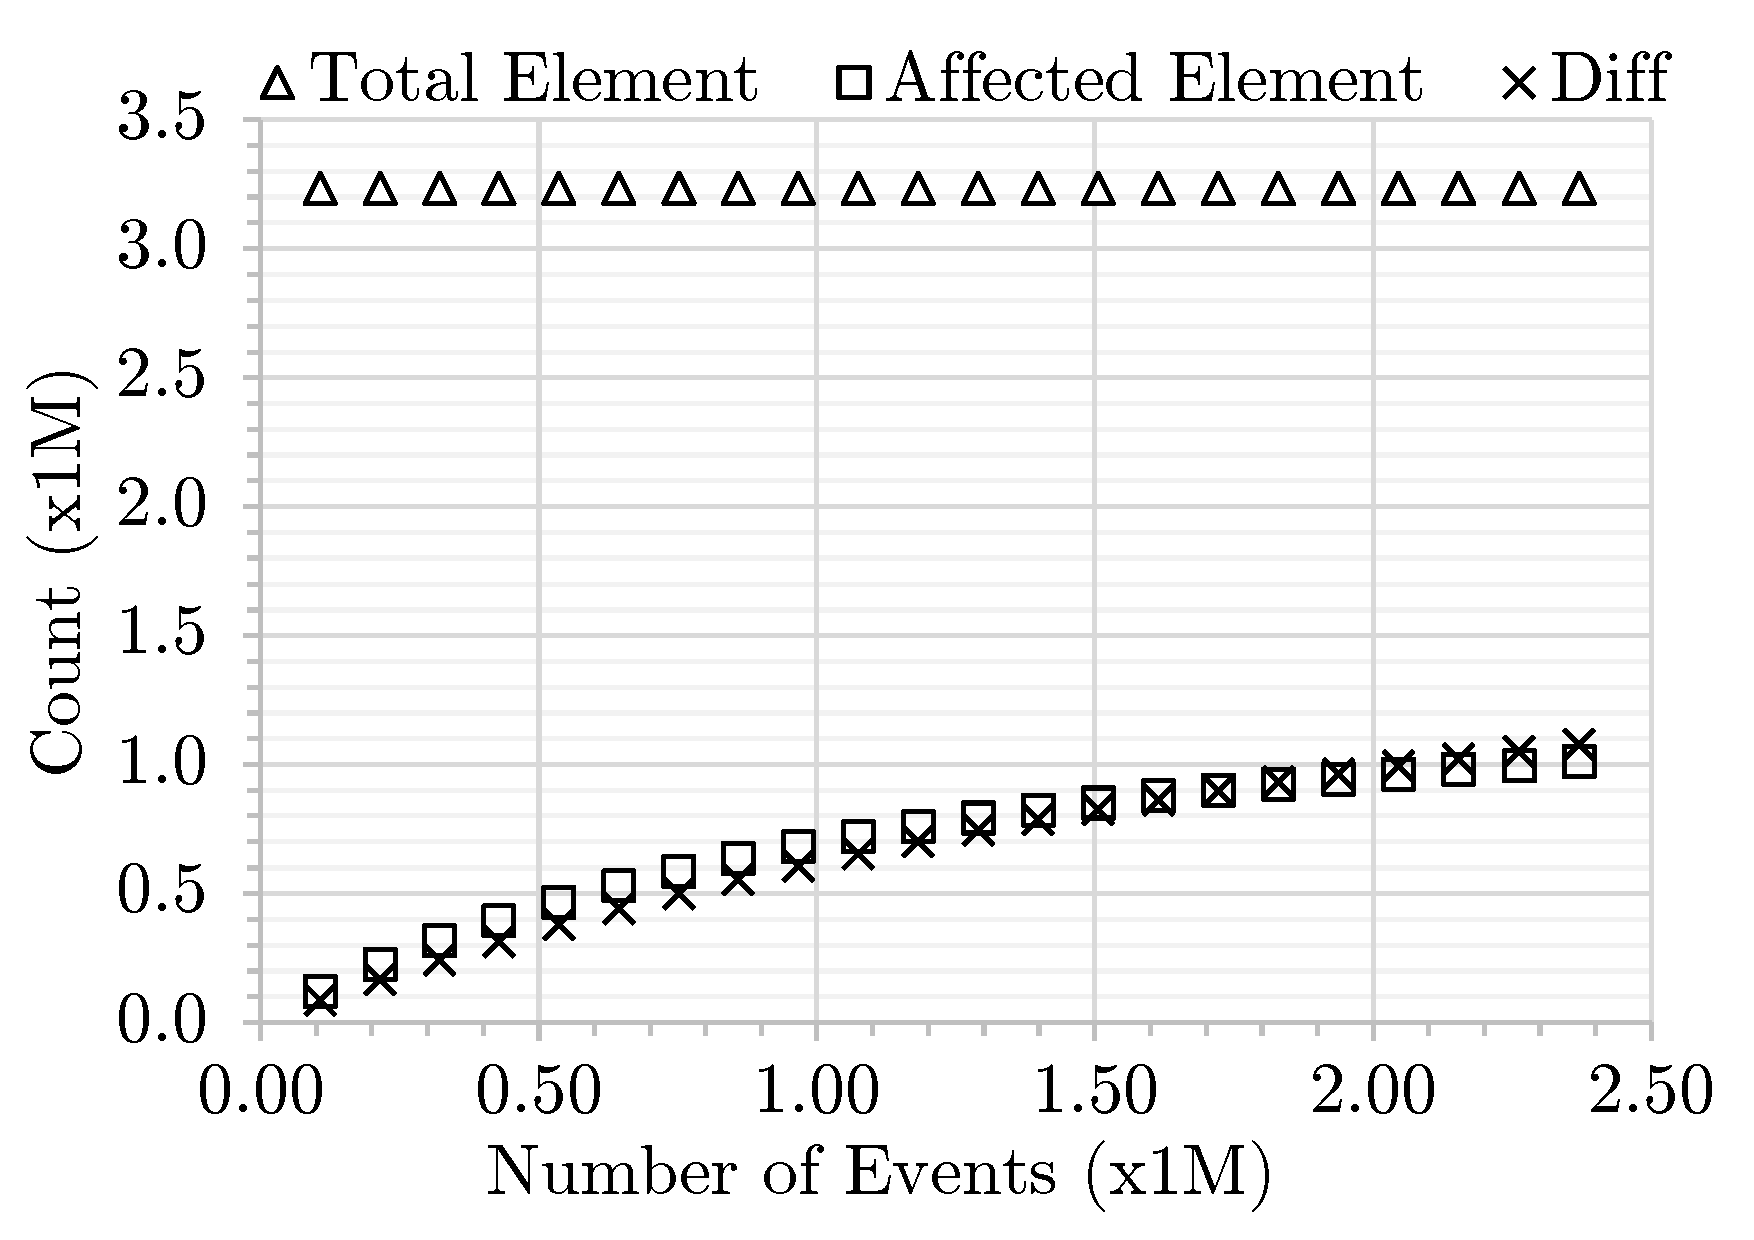
\includegraphics[width=\linewidth]{mixed-count-events}
  \caption{total elements, affected elements, and diffs}
  \label{fig:modification_course}
\end{wrapfigure}

This section reports on the obtained results in terms of comparison time and memory footprint for the mixed and homogeneous operation experiments. 


\vspace{-5pt}
\subsubsection{Mixed Operations}
\label{sec:mixed-operation}
In the mixed operation measurement, we modify two identical models differently by applying random operations. As the number of change events generated by the modification grows, the numbers of affected elements and differences also increase in a logarithmic manner. The patterns can be seen in Figure \ref{fig:modification_course}. The growth is logarithmic since the probability that the random operations modify the same elements also increases. Thus, some change events might not contribute to the addition of new affected elements and differences. In other words, more events are required to increase the number of affected elements or differences. In Figure \ref{fig:modification_course}, the total number of elements remains largely unchanged due to the equal probabilities of addition and deletion as has been set in Section \ref{sec:evaluation_6}. The figure gives us an insight about the characteristics of the modification caused by the random operations in the mixed operation measurement; it supports explaining the implication of the changes on execution time and memory footprints of model differencing.

\begin{figure}[ht]
  \begin{subfigure}[t]{0.495\linewidth}
    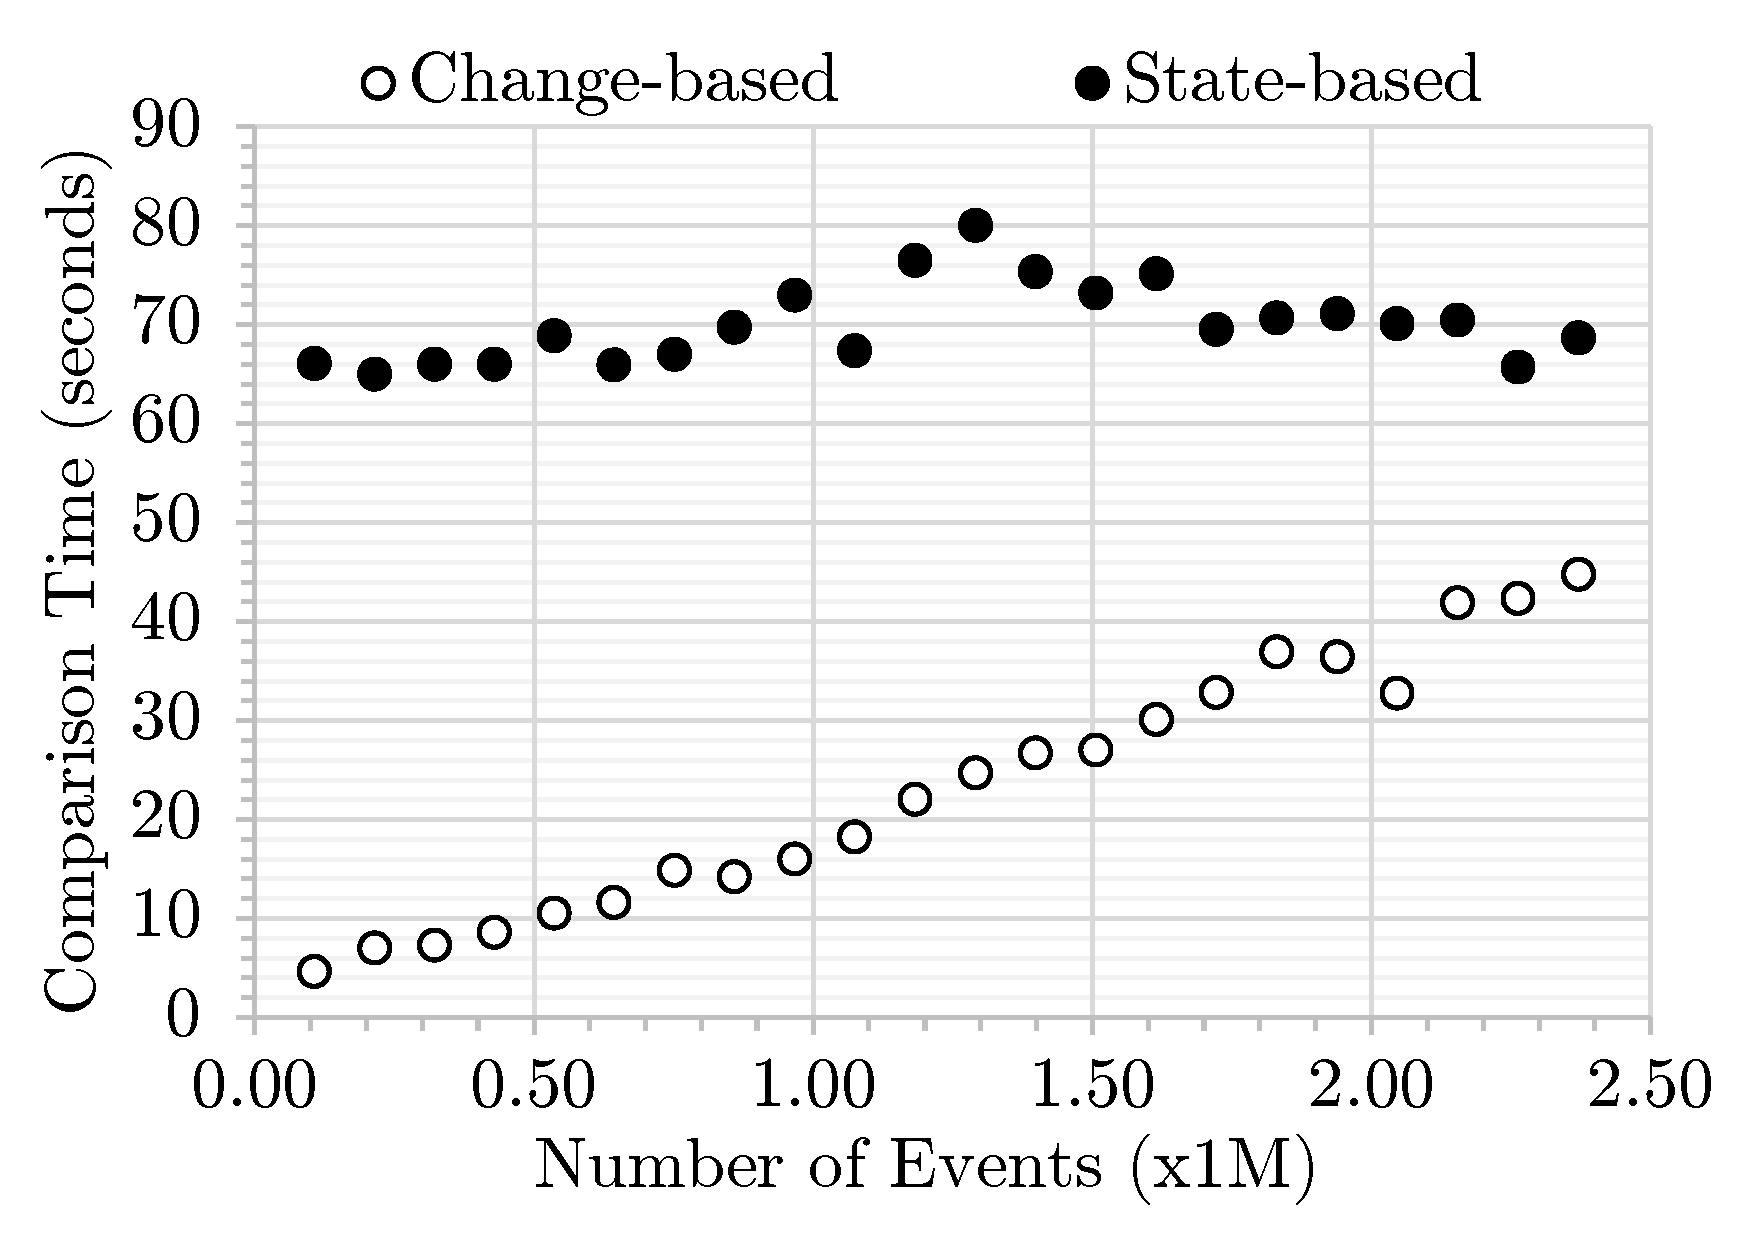
\includegraphics[width=\linewidth]{mixed-time-events}
    \caption{execution time}
    \label{fig:time_diffs}
  \end{subfigure}
  \begin{subfigure}[t]{0.495\linewidth}
    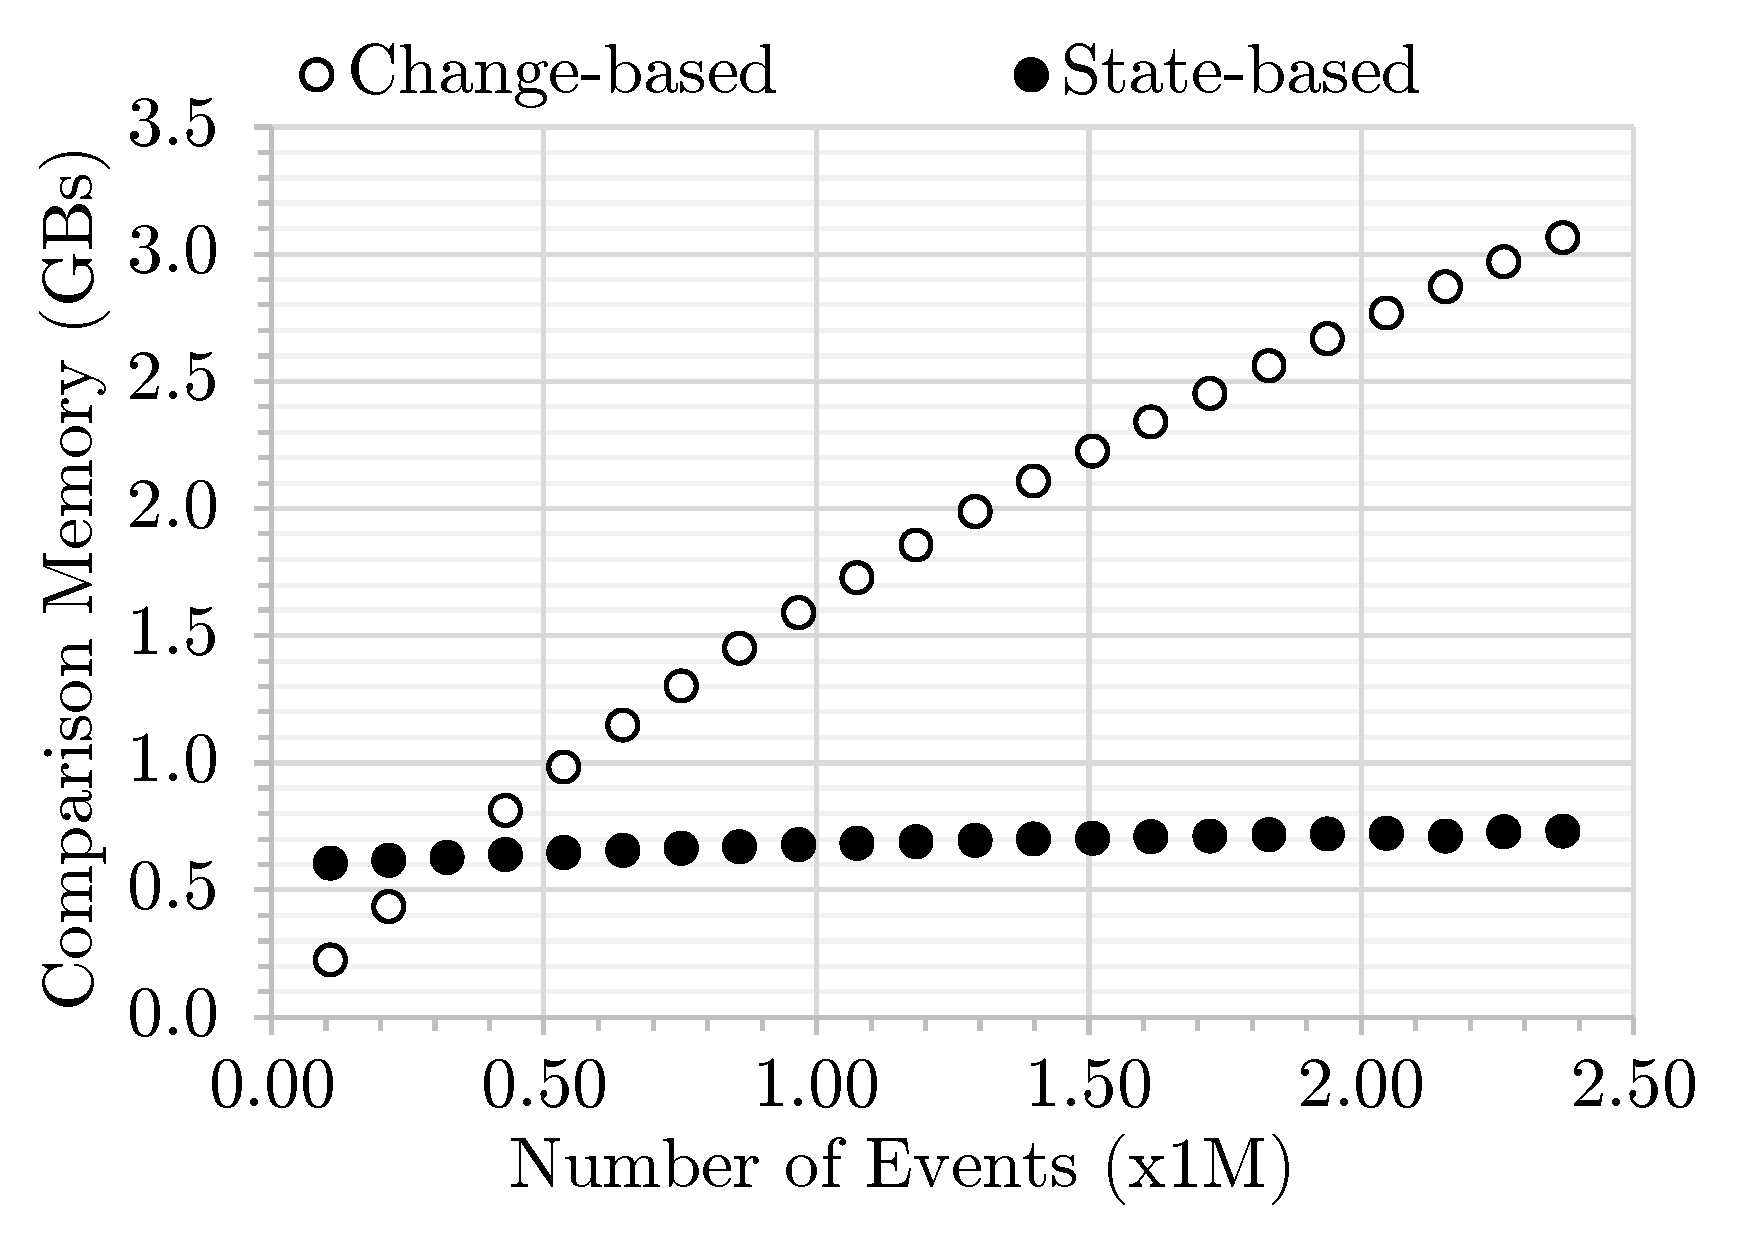
\includegraphics[width=\linewidth]{mixed-memory-events}
    \caption{memory footprint}
    \label{fig:memory_diffs}
  \end{subfigure}
  \caption{Change-based vs. state-based model differencing as differences increase.}
  \label{fig:change_vs_state}
\end{figure}


\begin{figure}[ht]
    \centering
    \begin{subfigure}[t]{0.495\linewidth}
        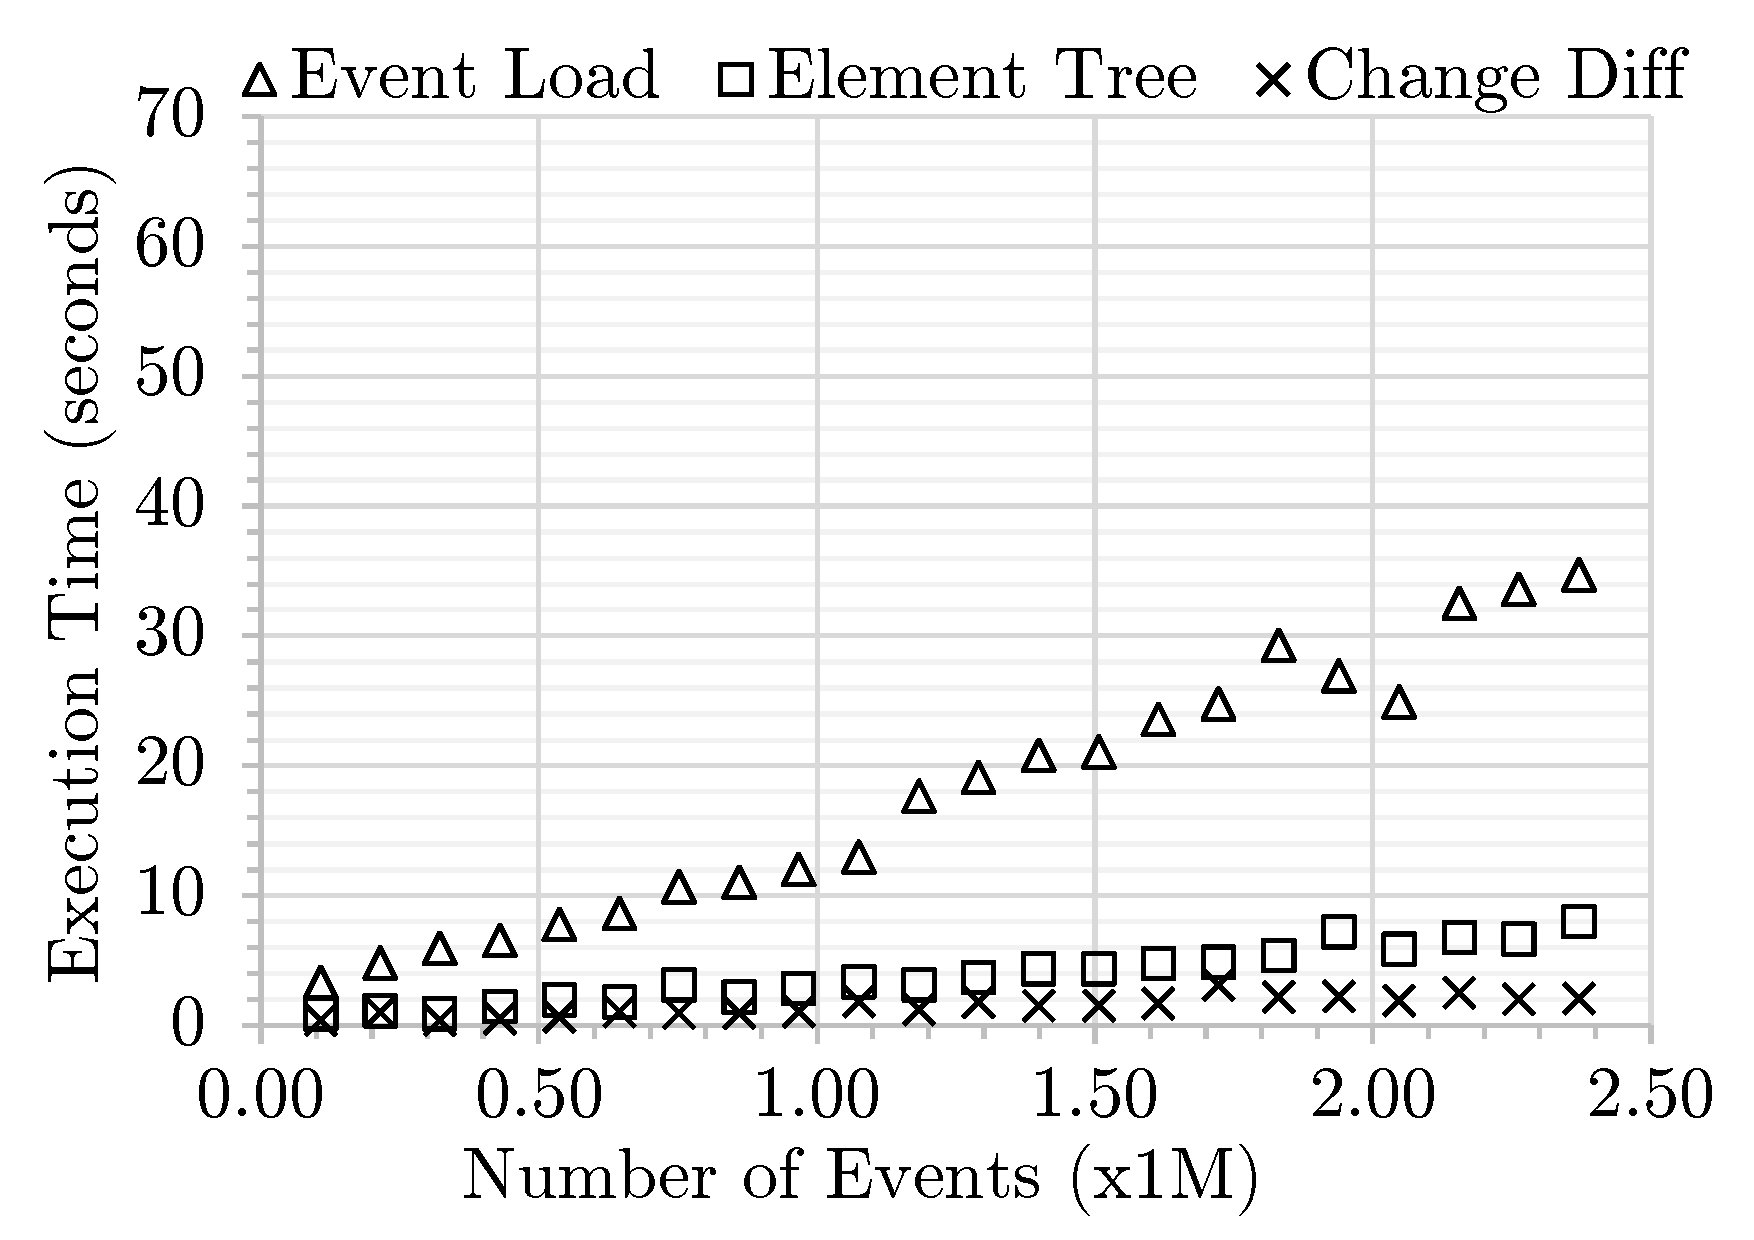
\includegraphics[width=\linewidth]{mixed-time-events-detail}
        \caption{change-based comparison time}
        \label{fig:time_changediff_detail}
    \end{subfigure}
    \hfill
    \begin{subfigure}[t]{0.495\linewidth}
        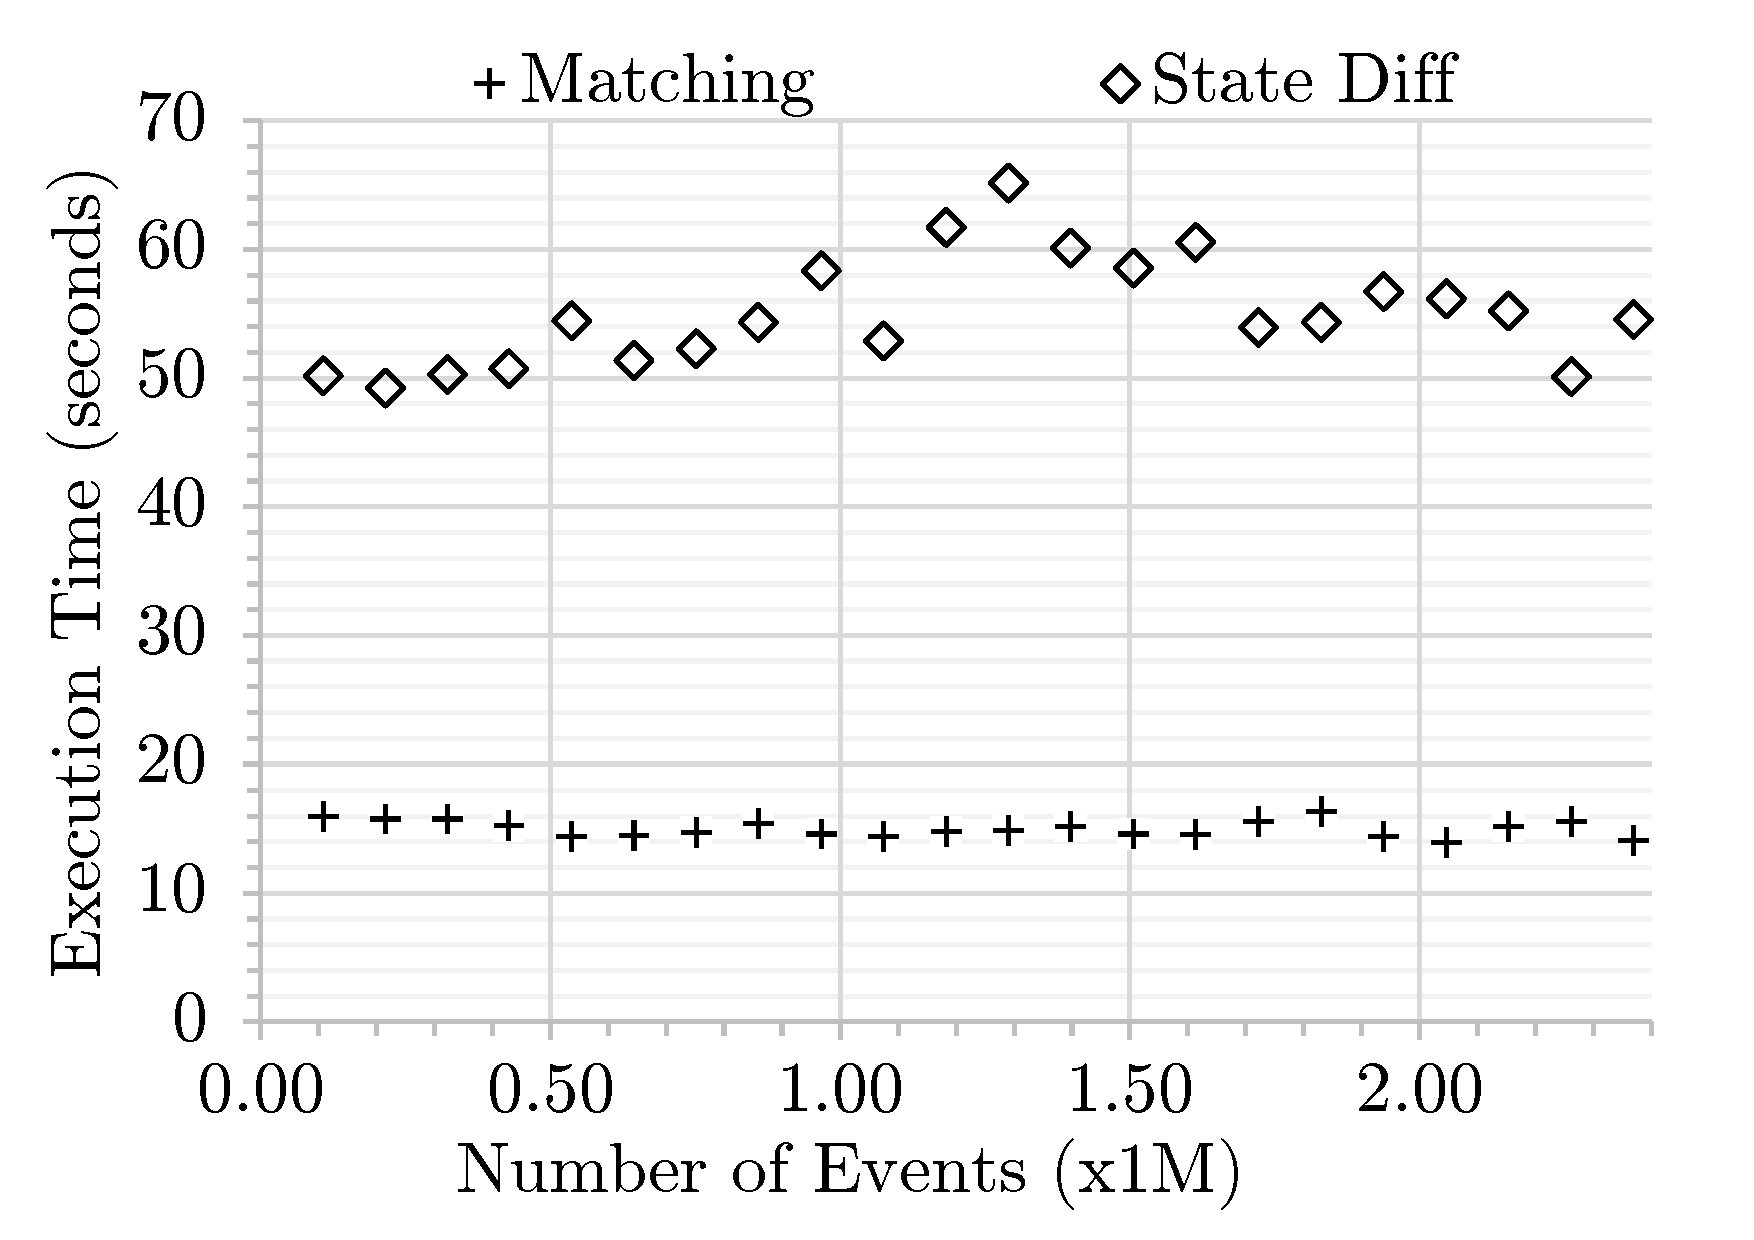
\includegraphics[width=\linewidth]{state-time-events-detail}
        \caption{state-based comparison time}
        \label{fig:time_statediff_detail}
    \end{subfigure}
    \begin{subfigure}[t]{0.495\linewidth}
        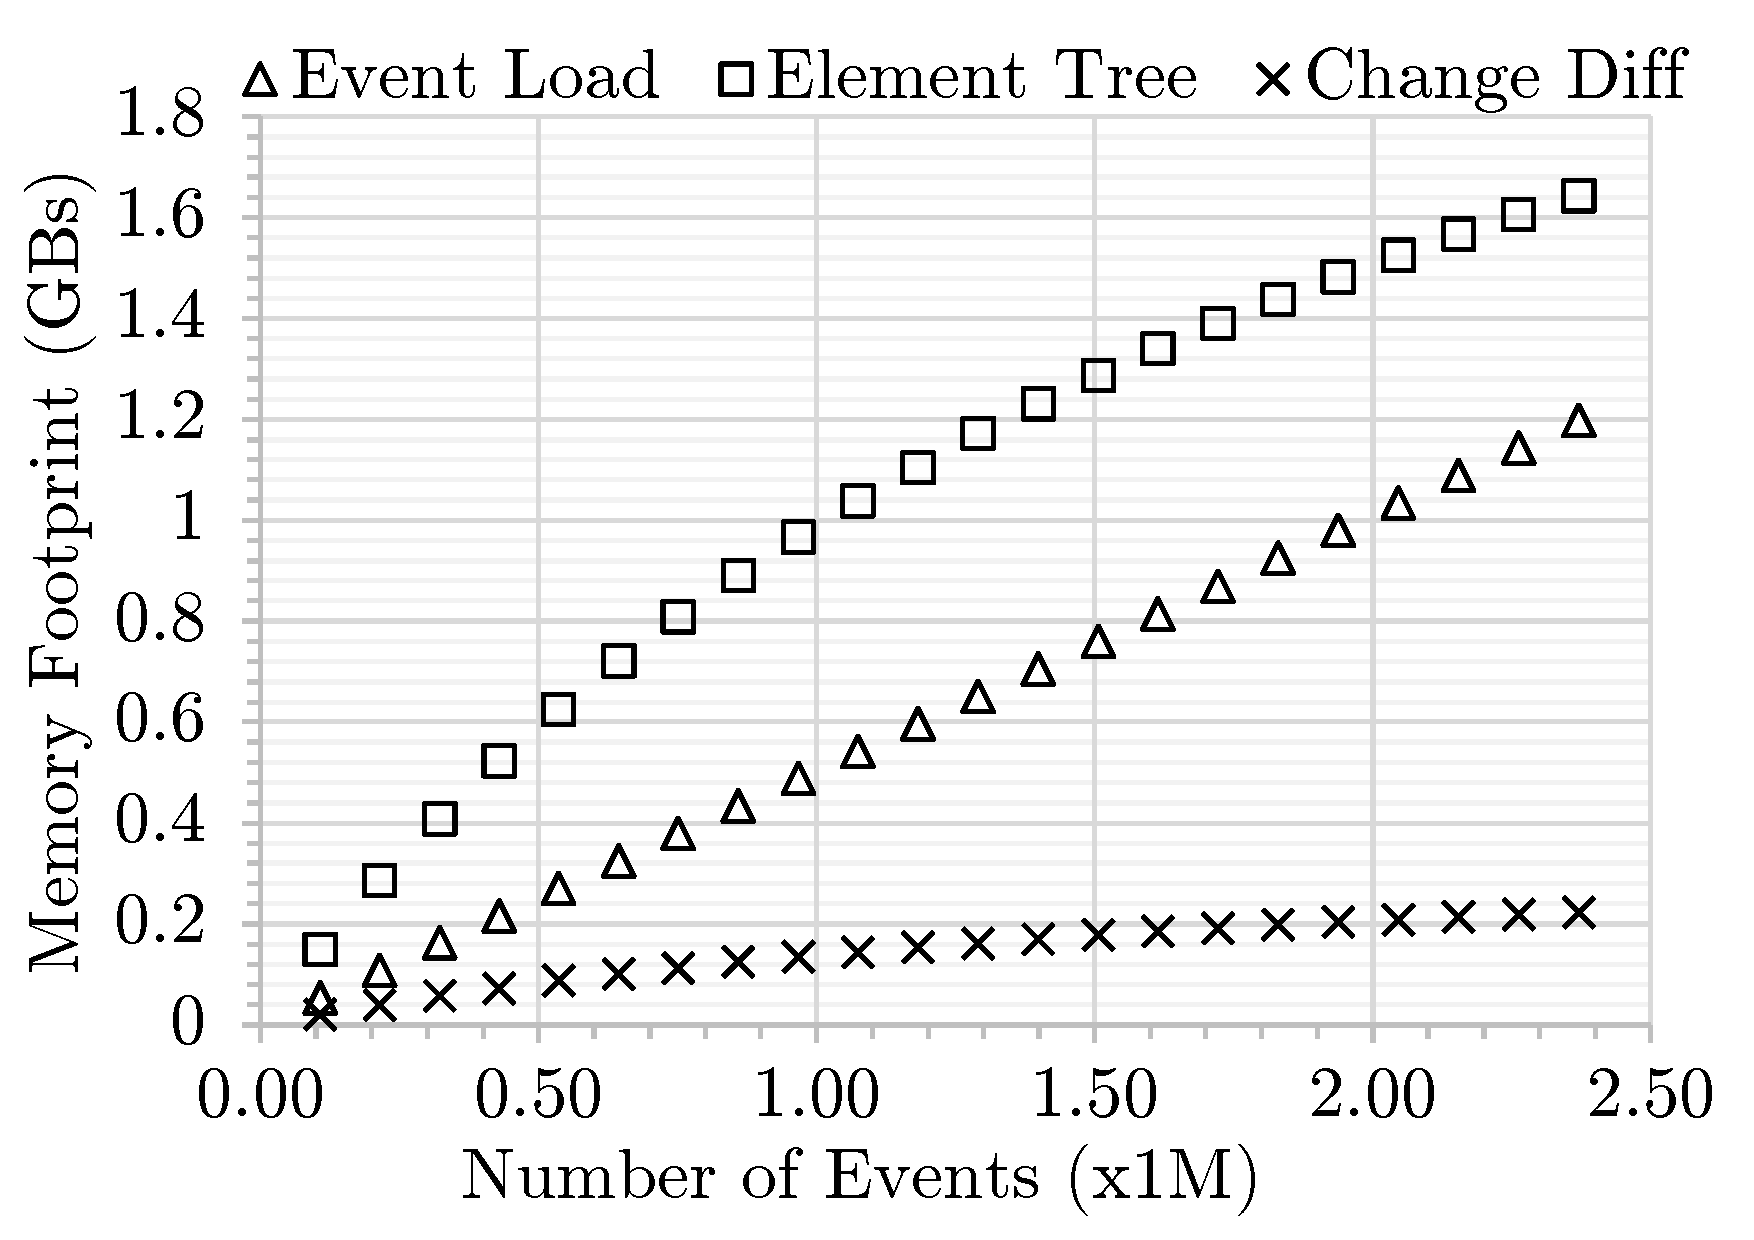
\includegraphics[width=\linewidth]{mixed-memory-events-detail}
        \caption{change-based memory footprint}
        \label{fig:memory_changediff_detail}
    \end{subfigure}
    \hfill
    \begin{subfigure}[t]{0.495\linewidth}
        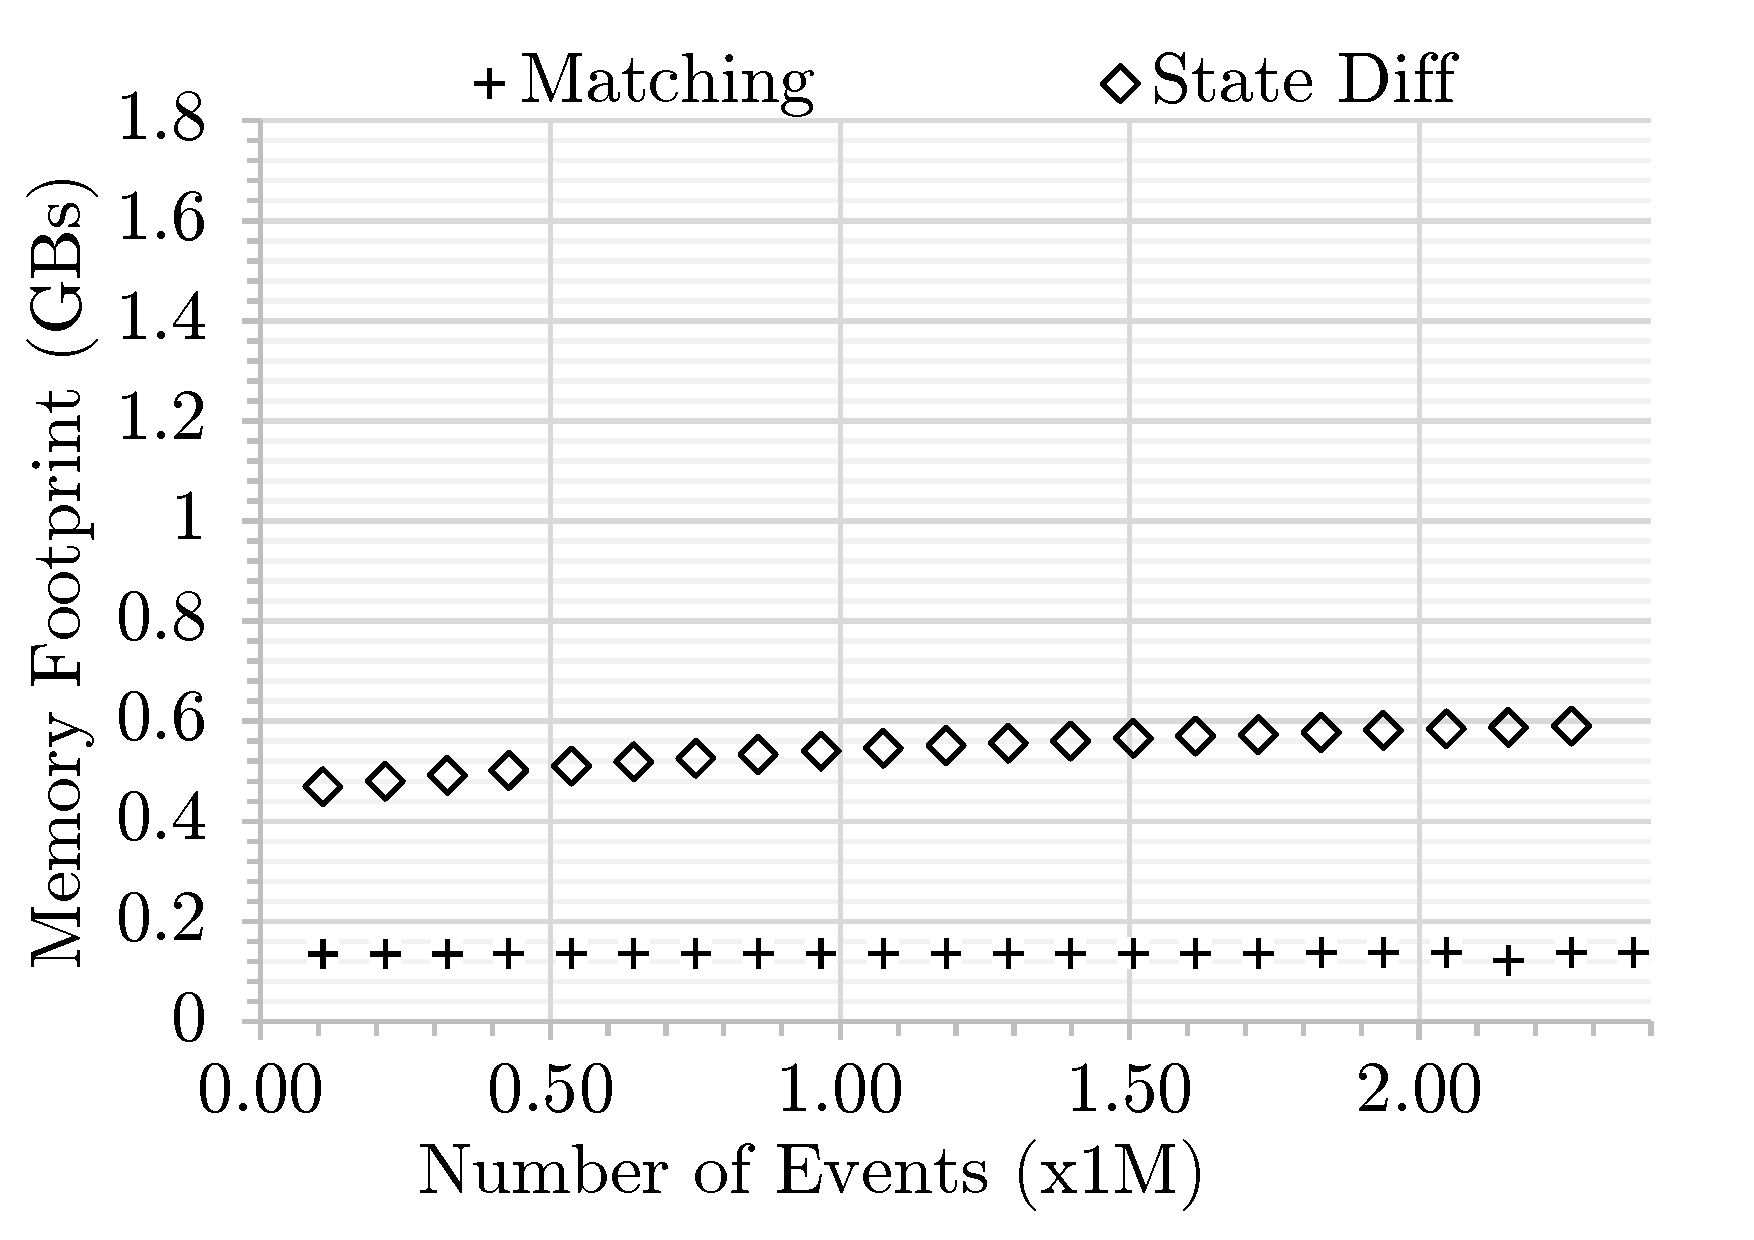
\includegraphics[width=\linewidth]{state-memory-events-detail}
        \caption{state-based memory footprint}
        \label{fig:memory_statediff_detail}
    \end{subfigure}
    \caption{Breakdown view of comparison time and memory footprint in Figure \ref{fig:change_vs_state}.}
    \label{fig:time_memory_detail}
\end{figure}

After applying some random changes on both models, the modification produces 100,000 change events at the first measurement point. Using this amount of events, our change-based comparison only takes 5 seconds to identify around 90,000 differences, in contrast to the state-based comparison that takes 66 seconds (see the first measurement points in Figures \ref{fig:modification_course} and \ref{fig:time_diffs}). If the modification continues, more change events are generated. This growing number of change events has to be loaded into memory and thus slows down the change-based comparison. Nevertheless, the change-based comparison is still faster than the state-based comparison even though the number of change events reaches 2.37 million -- more than 1 million differences at that point; the change-based comparison outperforms the state-based comparison in execution time (Figure \ref{fig:time_diffs}). Figure \ref{fig:time_changediff_detail} breaks down the comparison time in detail. It exhibits that the event loading time is the dominant contributor to the slowdown compared to the element tree's construction time and diffing time. 

For the state-based comparison in Figure \ref{fig:time_statediff_detail}, the comparison time only experiences a slight increase as the number of identified differences also grows.
%\dk{Change to ``grows''?}. 
This slight increase is contributed mainly by the diffing time, while the matching time tends to be constant due to the very small increase of the total elements (Figures \ref{fig:modification_course}).

Nevertheless, change-based comparison generally consumes more memory than the state-based comparison (see Figure \ref{fig:memory_diffs}). It only consumes less memory than its state-based counterpart when the number of events is less than 0.3 million (around less than 0.25 million identified differences at that moment). Figure \ref{fig:memory_changediff_detail} breaks down the memory footprint of change-based comparison into three factors: the loaded change events, element tree, and diffs. As modification continues, an increasing number of events is generated. These events have to be loaded into memory since they contain the required information for the construction of an element tree. The amount of space to keep these change events in memory grows linearly with their number. 

\begin{figure}[ht]
  \centering
  \begin{subfigure}[t]{0.495\linewidth}
    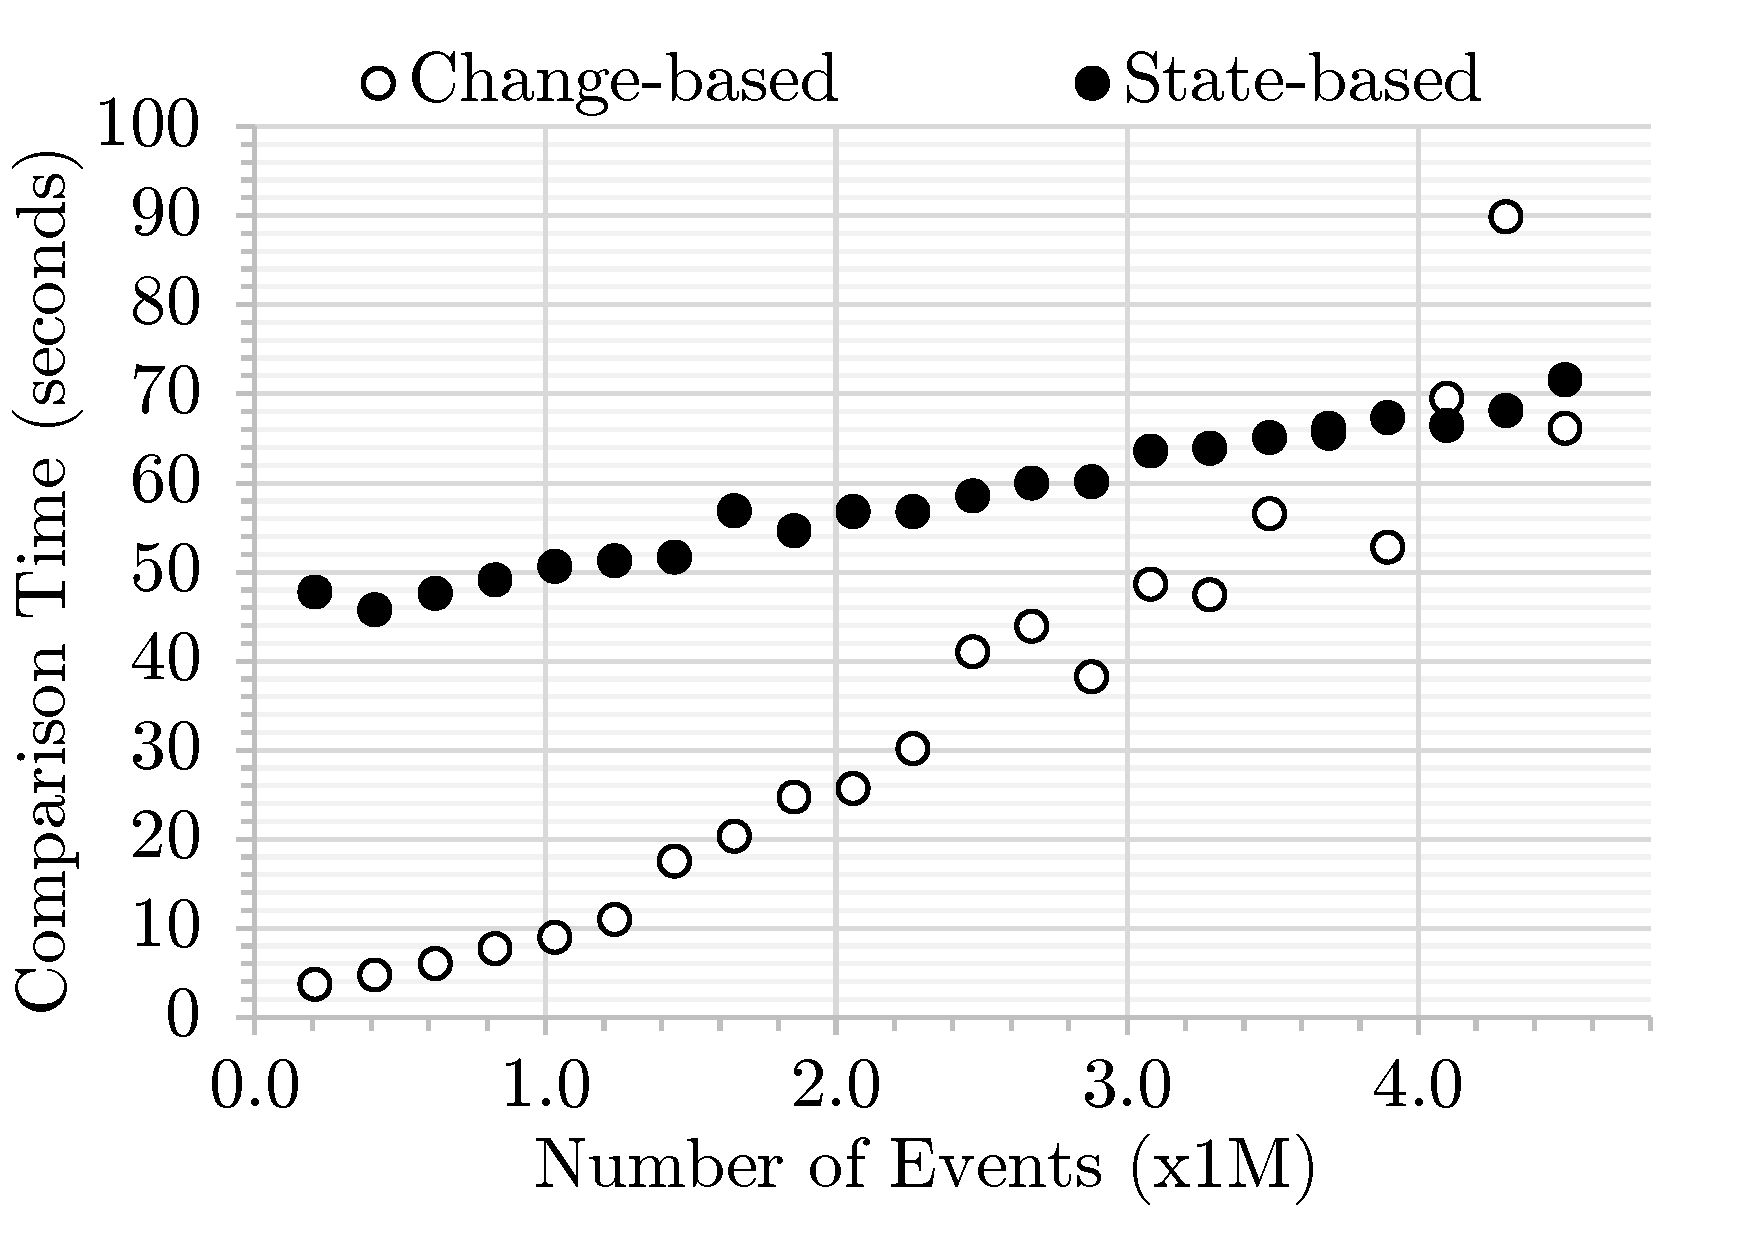
\includegraphics[width=\linewidth]{add-time-events}
    \caption{add-only}
    \label{fig:add-time-events}
  \end{subfigure}
  \hfill
  \begin{subfigure}[t]{0.495\linewidth}
    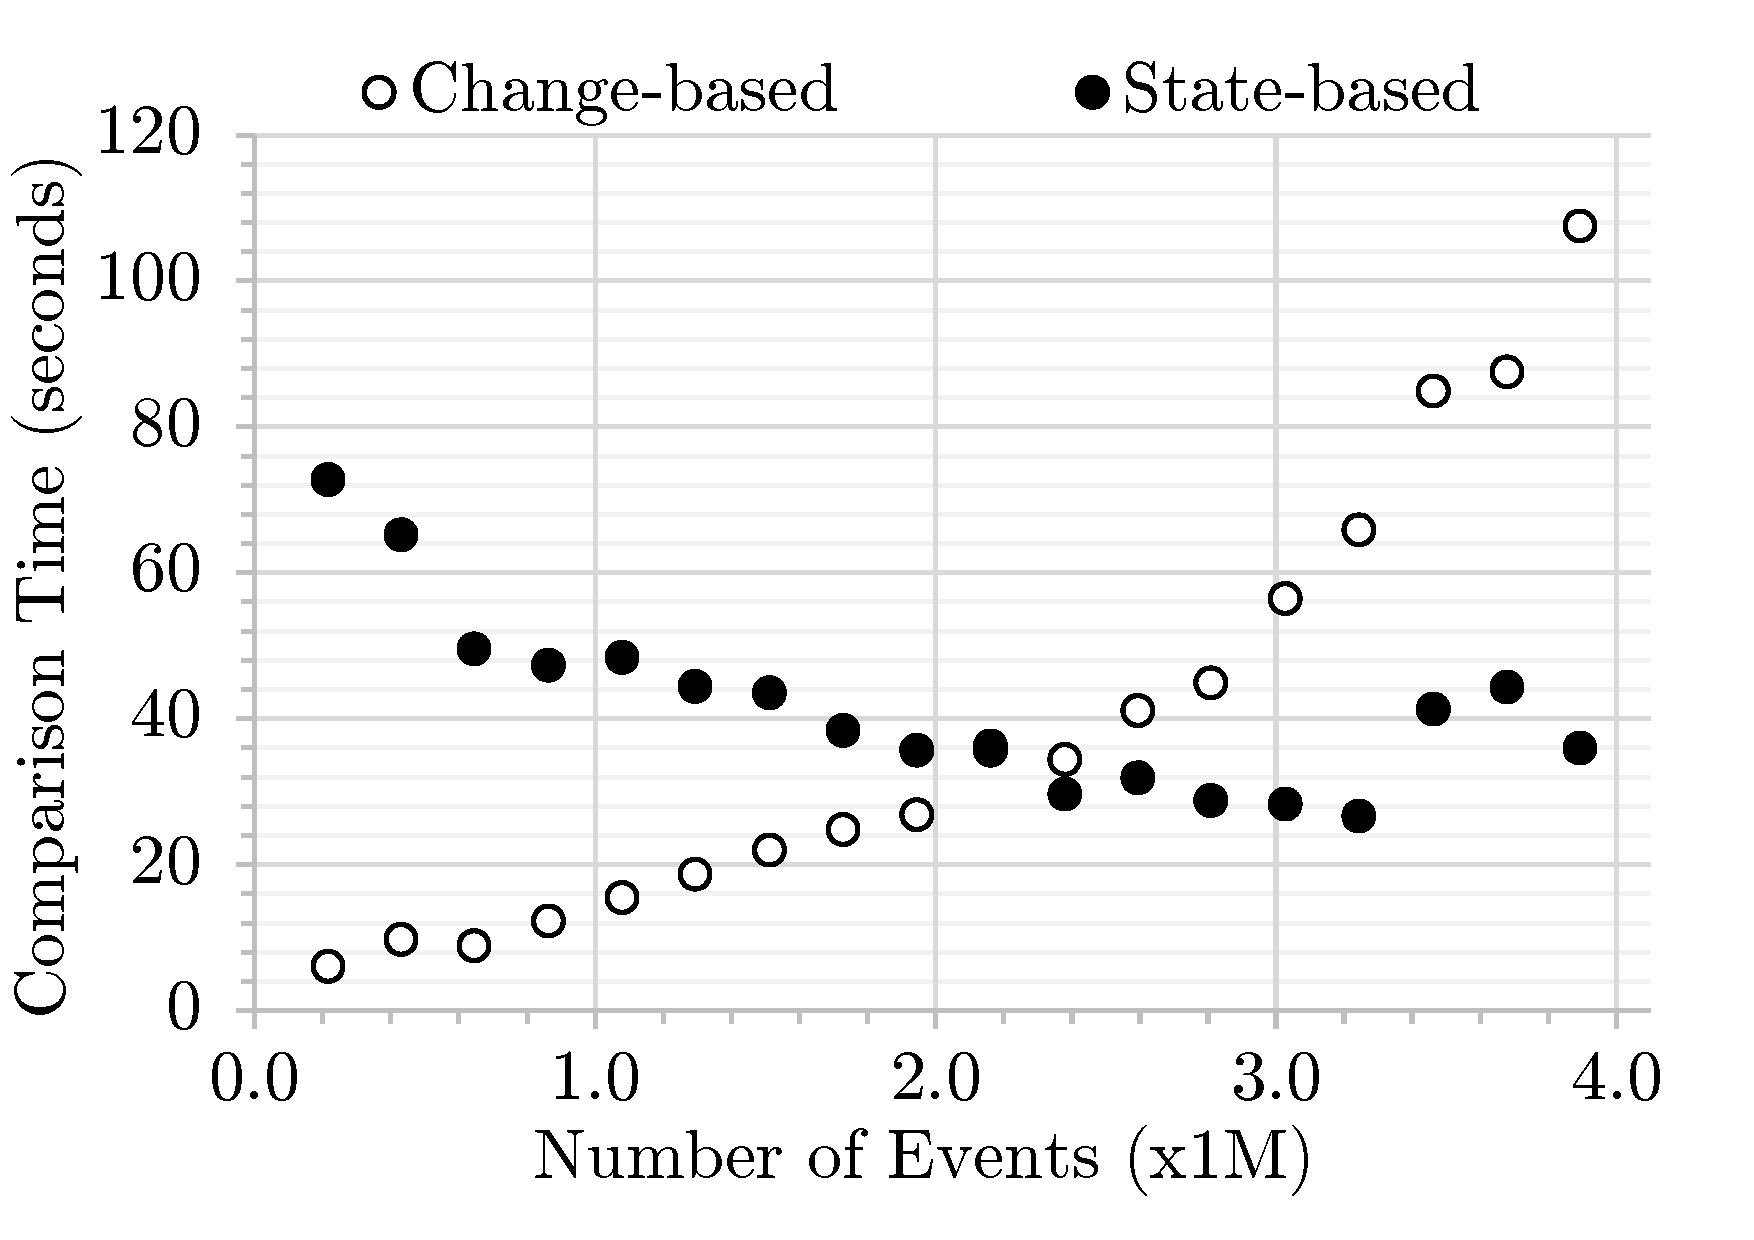
\includegraphics[width=\linewidth]{delete-time-events}
    \caption{delete-only}
    \label{fig:delete-time-events}
  \end{subfigure}
  \begin{subfigure}[t]{0.495\linewidth}
    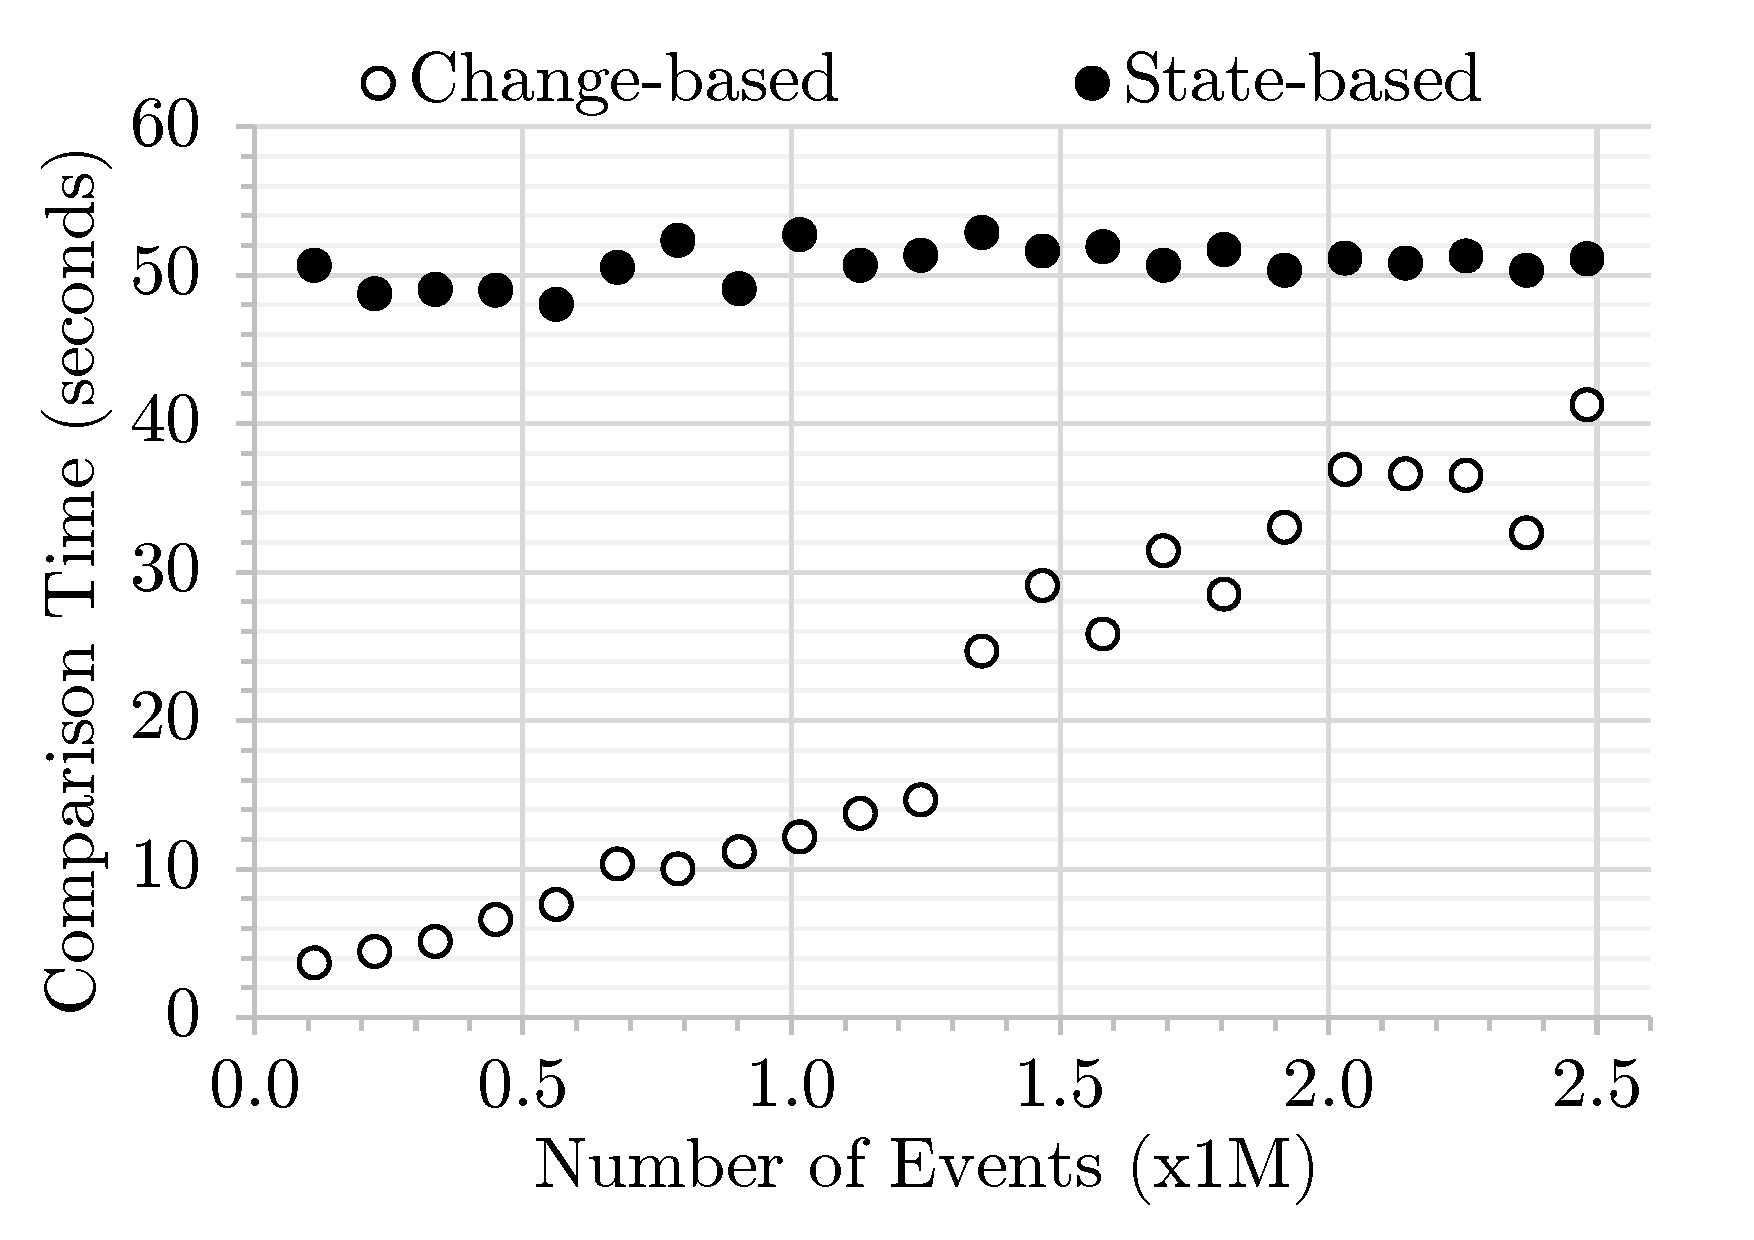
\includegraphics[width=\linewidth]{move-time-events}
    \caption{move-only}
    \label{fig:move-time-events}
  \end{subfigure}
  \hfill
  \begin{subfigure}[t]{0.495\linewidth}
    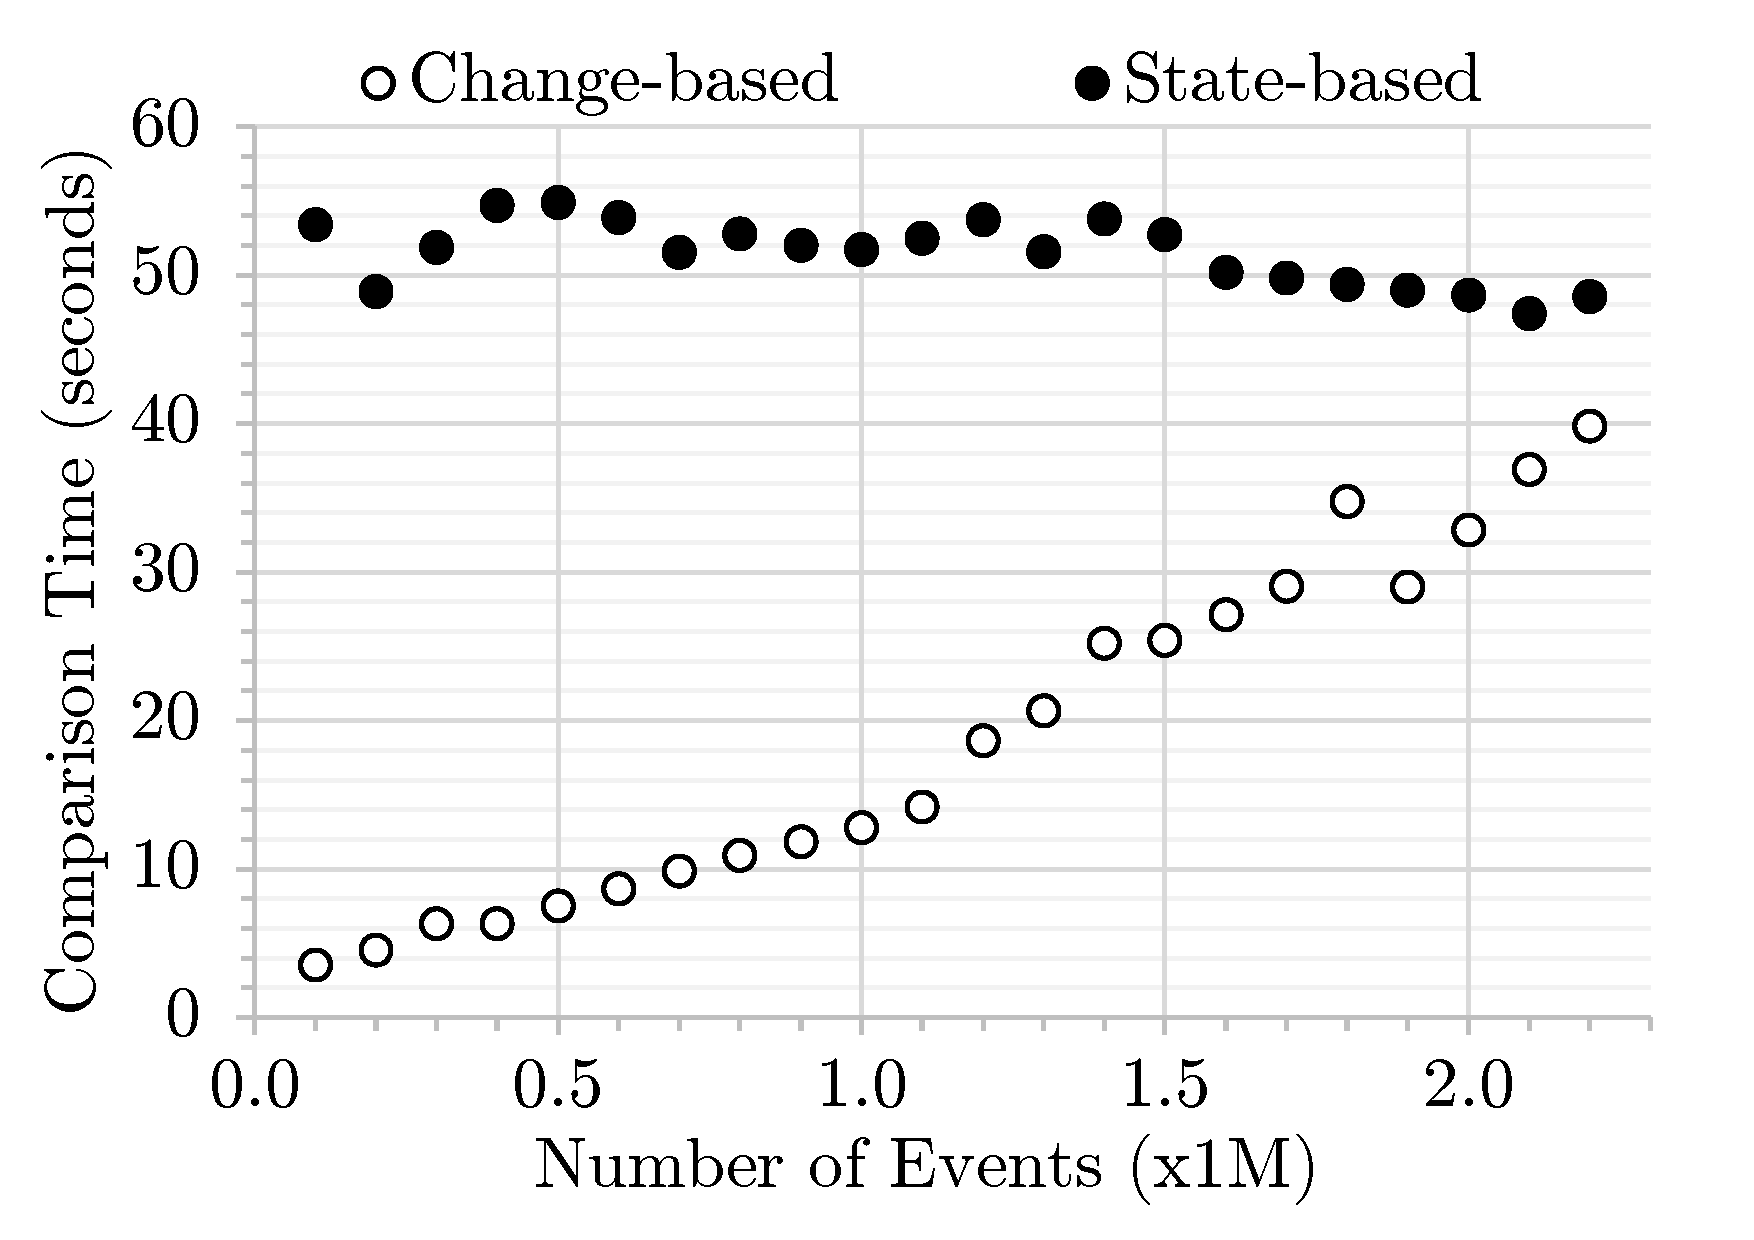
\includegraphics[width=\linewidth]{change-time-events}
    \caption{change-only}
    \label{fig:change-time-events}
  \end{subfigure}
  \caption{Comparison time for homogeneous operations.}
  \label{fig:operation_time_events}
\end{figure}

In contrast, the memory used for the element tree grows logarithmically. As the number of events increases, the probability that events modify already affected elements also increases. Thus, no additional memory allocation is required for the element tree. We can also notice that the element tree occupies most of the memory footprint since it mirrors the partial states -- elements, features, and values -- of the models that are affected by the changes. Moreover, in our technical implementation, a feature can have many instances -- one instance for each element (As a comparison, in the EMF implementation, there is only one instance for a feature. The feature is used as a key so that different elements can have the same feature that maps to different values simultaneously). This contributes to the large memory footprint used by the element tree. The identified change-based diffs, the third factor, are the smallest factor that contributes to the memory footprint of the change-based comparison. 

For the state-based comparison in Figure \ref{fig:memory_statediff_detail}, the memory footprint only grows slightly along the increase of differences. A large part of the memory footprint is used to represent the identified differences, while the memory used for matches tends to be constant as the changes of the total elements are very small -- less new elements means less memory needs to be allocated for new matches (Figures \ref{fig:modification_course}). 

\subsubsection{Homogeneous Operations}
\label{sec:homogeneous-operation}



\begin{figure}[ht]
    \centering
    \begin{subfigure}[t]{0.495\linewidth}
        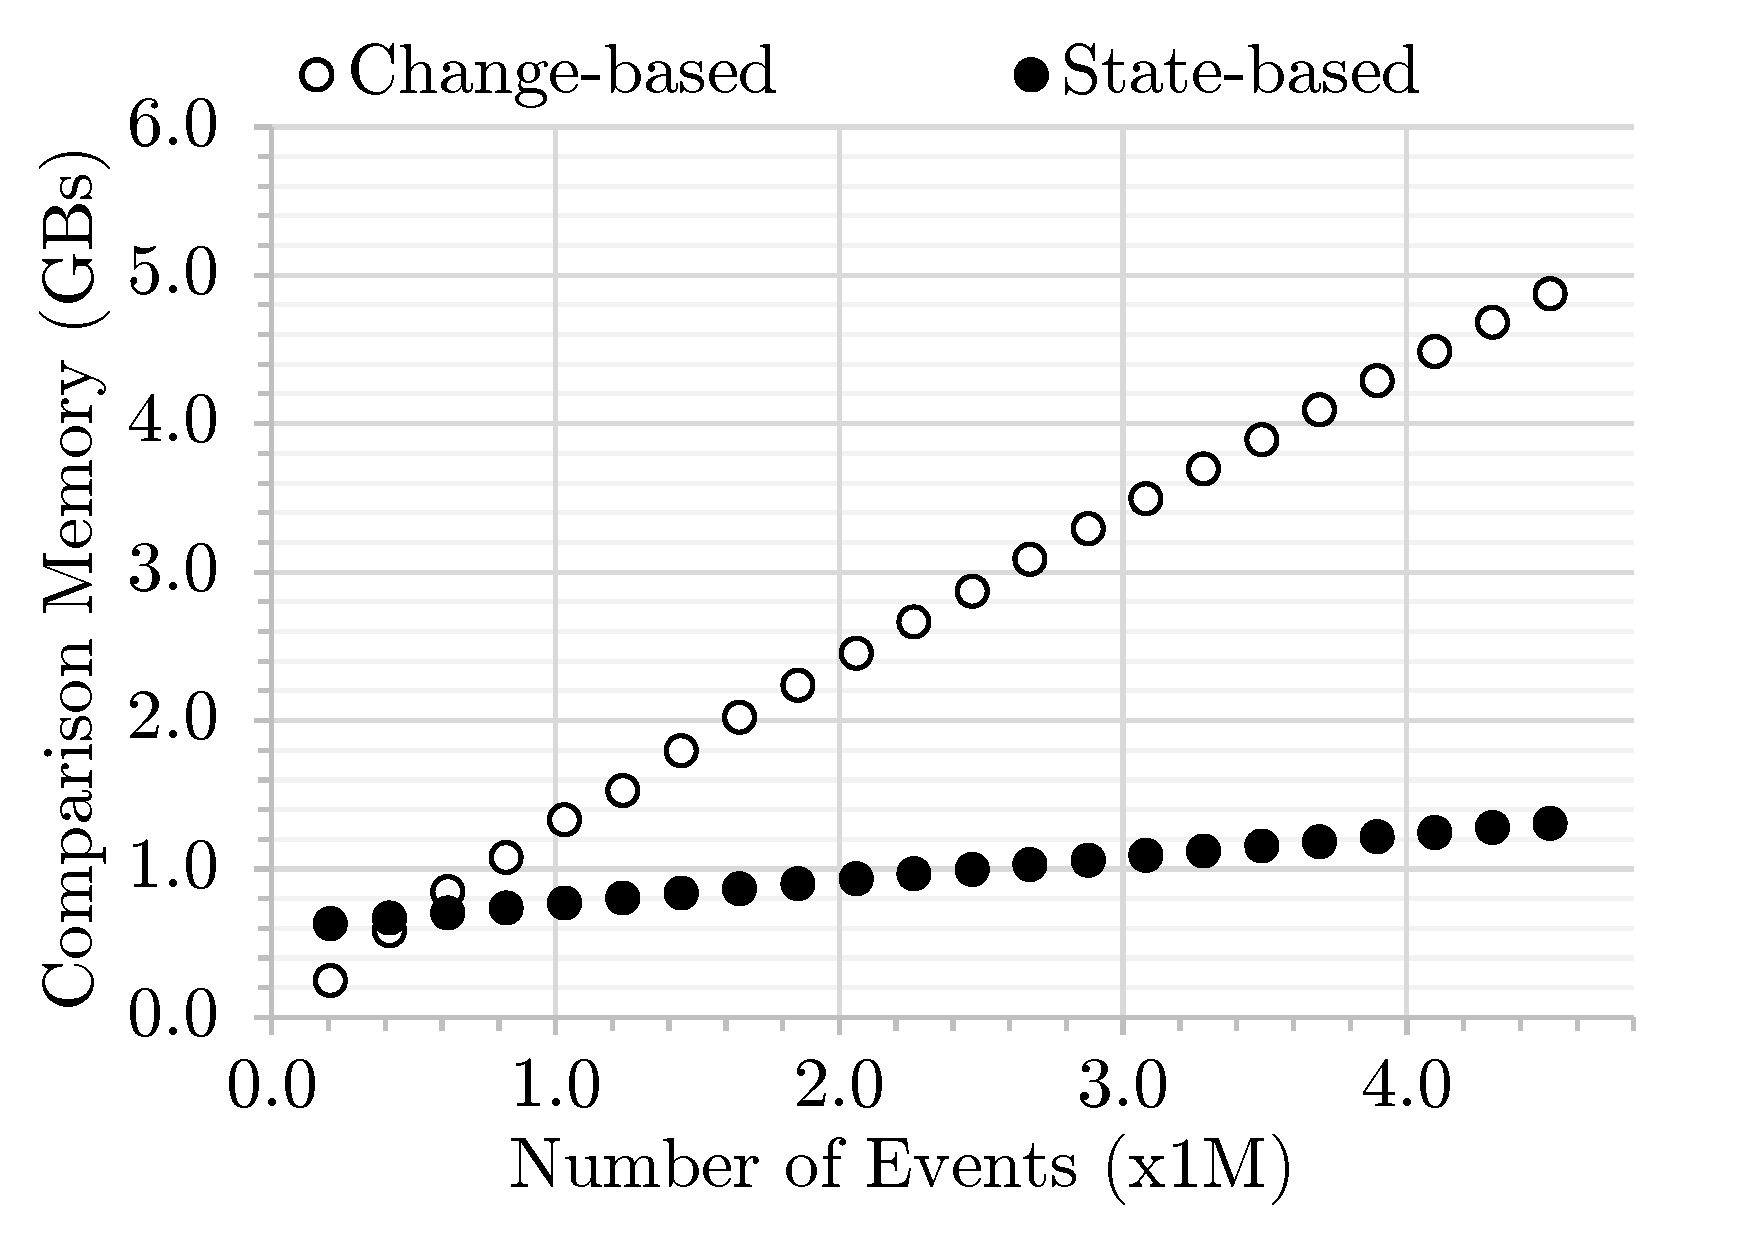
\includegraphics[width=\linewidth]{add-memory-events}
        \caption{add-only}
        \label{fig:add-memory-events}
    \end{subfigure}
    \hfill
    \begin{subfigure}[t]{0.495\linewidth}
        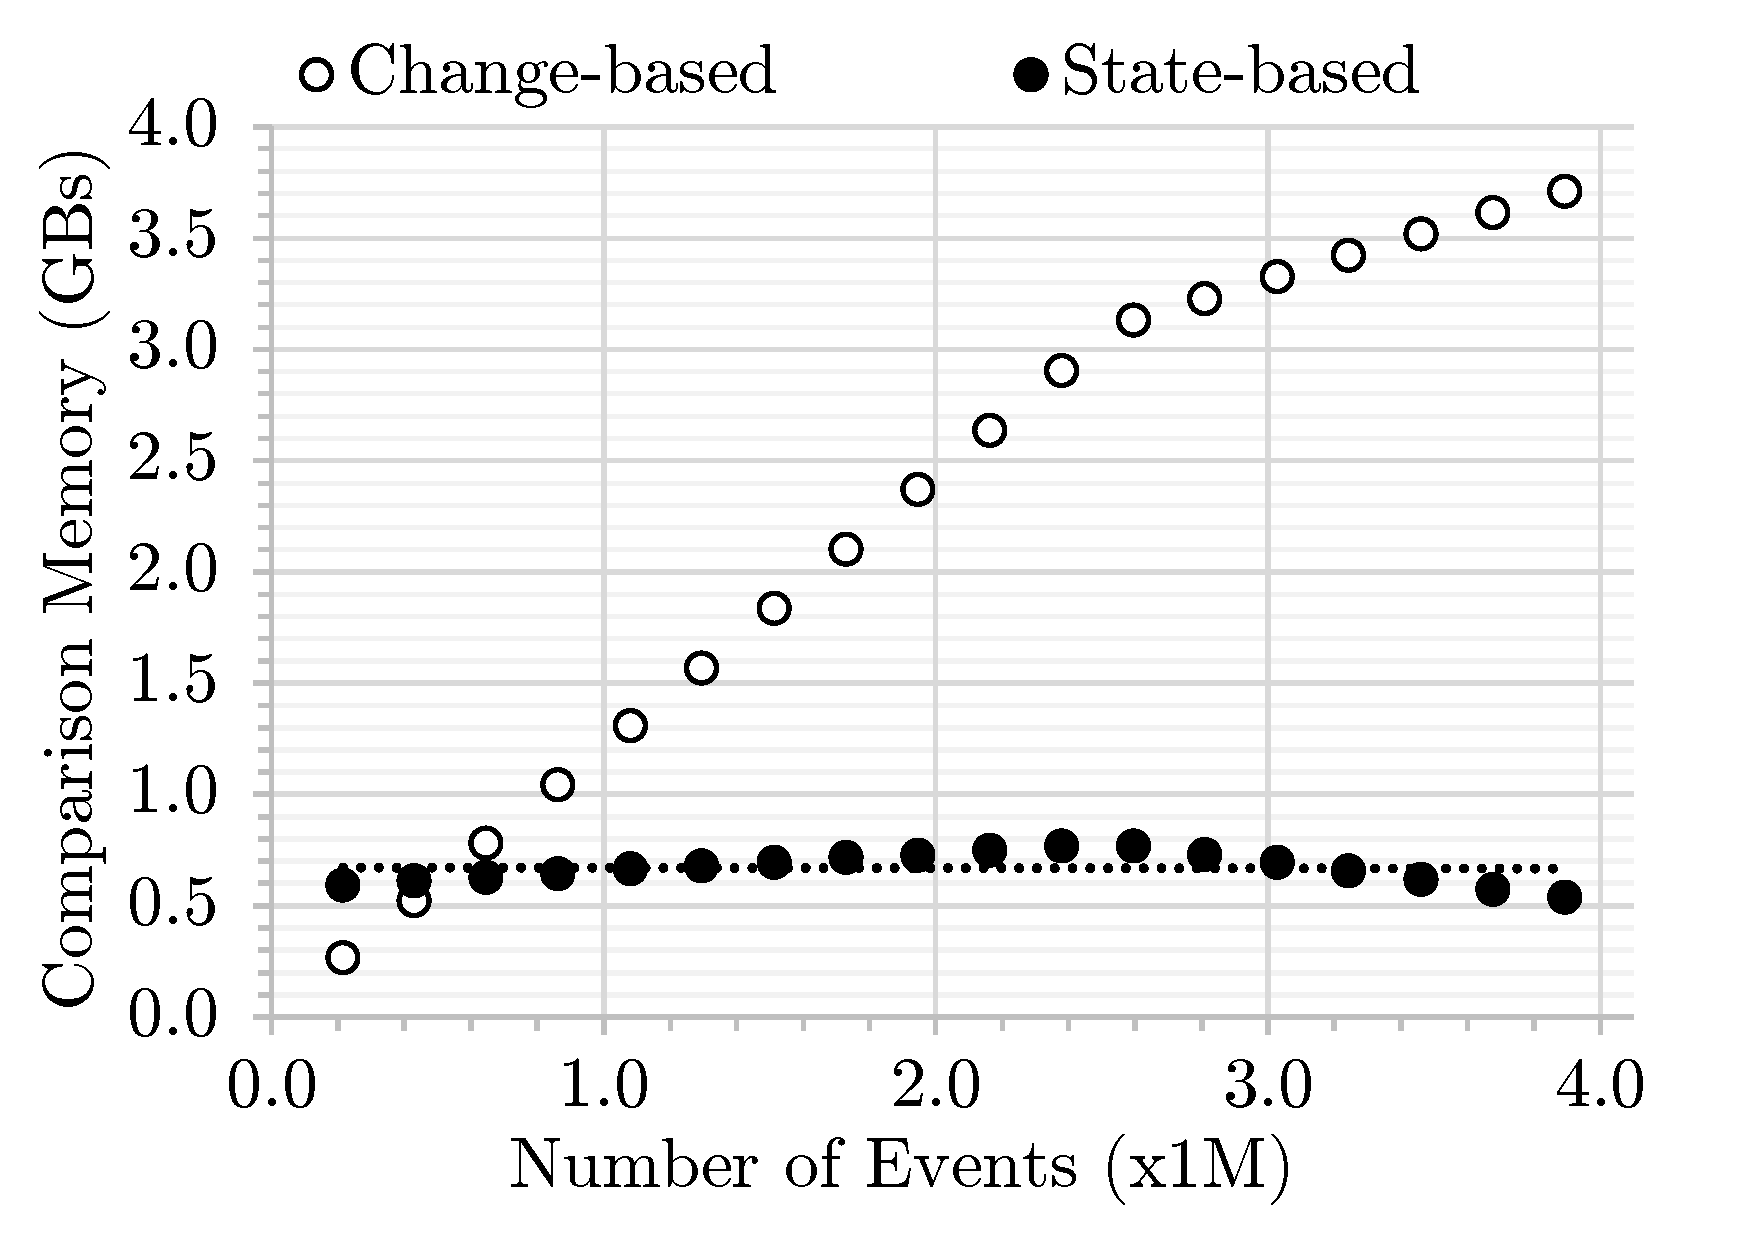
\includegraphics[width=\linewidth]{delete-memory-events}
        \caption{delete-only}
        \label{fig:delete-memory-events}
    \end{subfigure}
    \begin{subfigure}[t]{0.495\linewidth}
        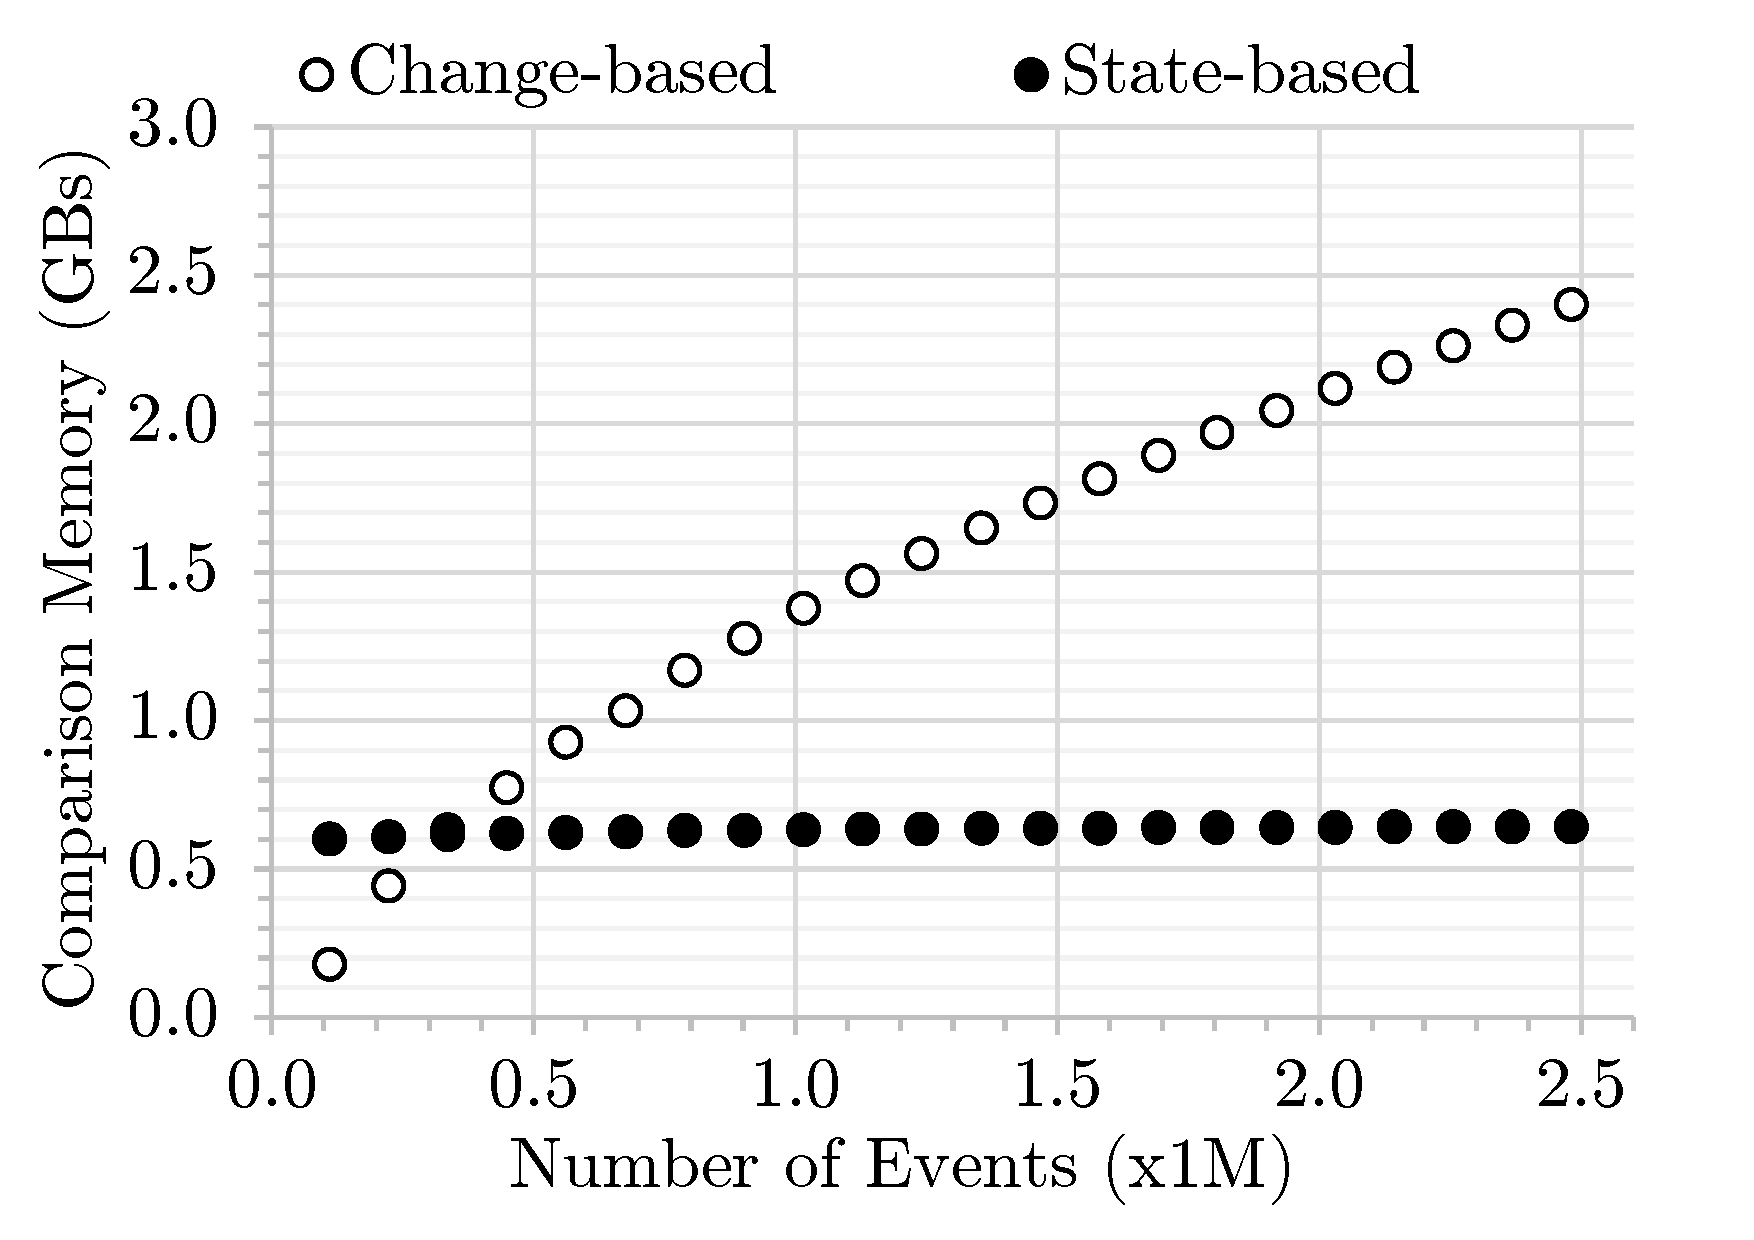
\includegraphics[width=\linewidth]{move-memory-events}
        \caption{move-only}
        \label{fig:move-memory-events}
    \end{subfigure}
    \hfill
    \begin{subfigure}[t]{0.495\linewidth}
        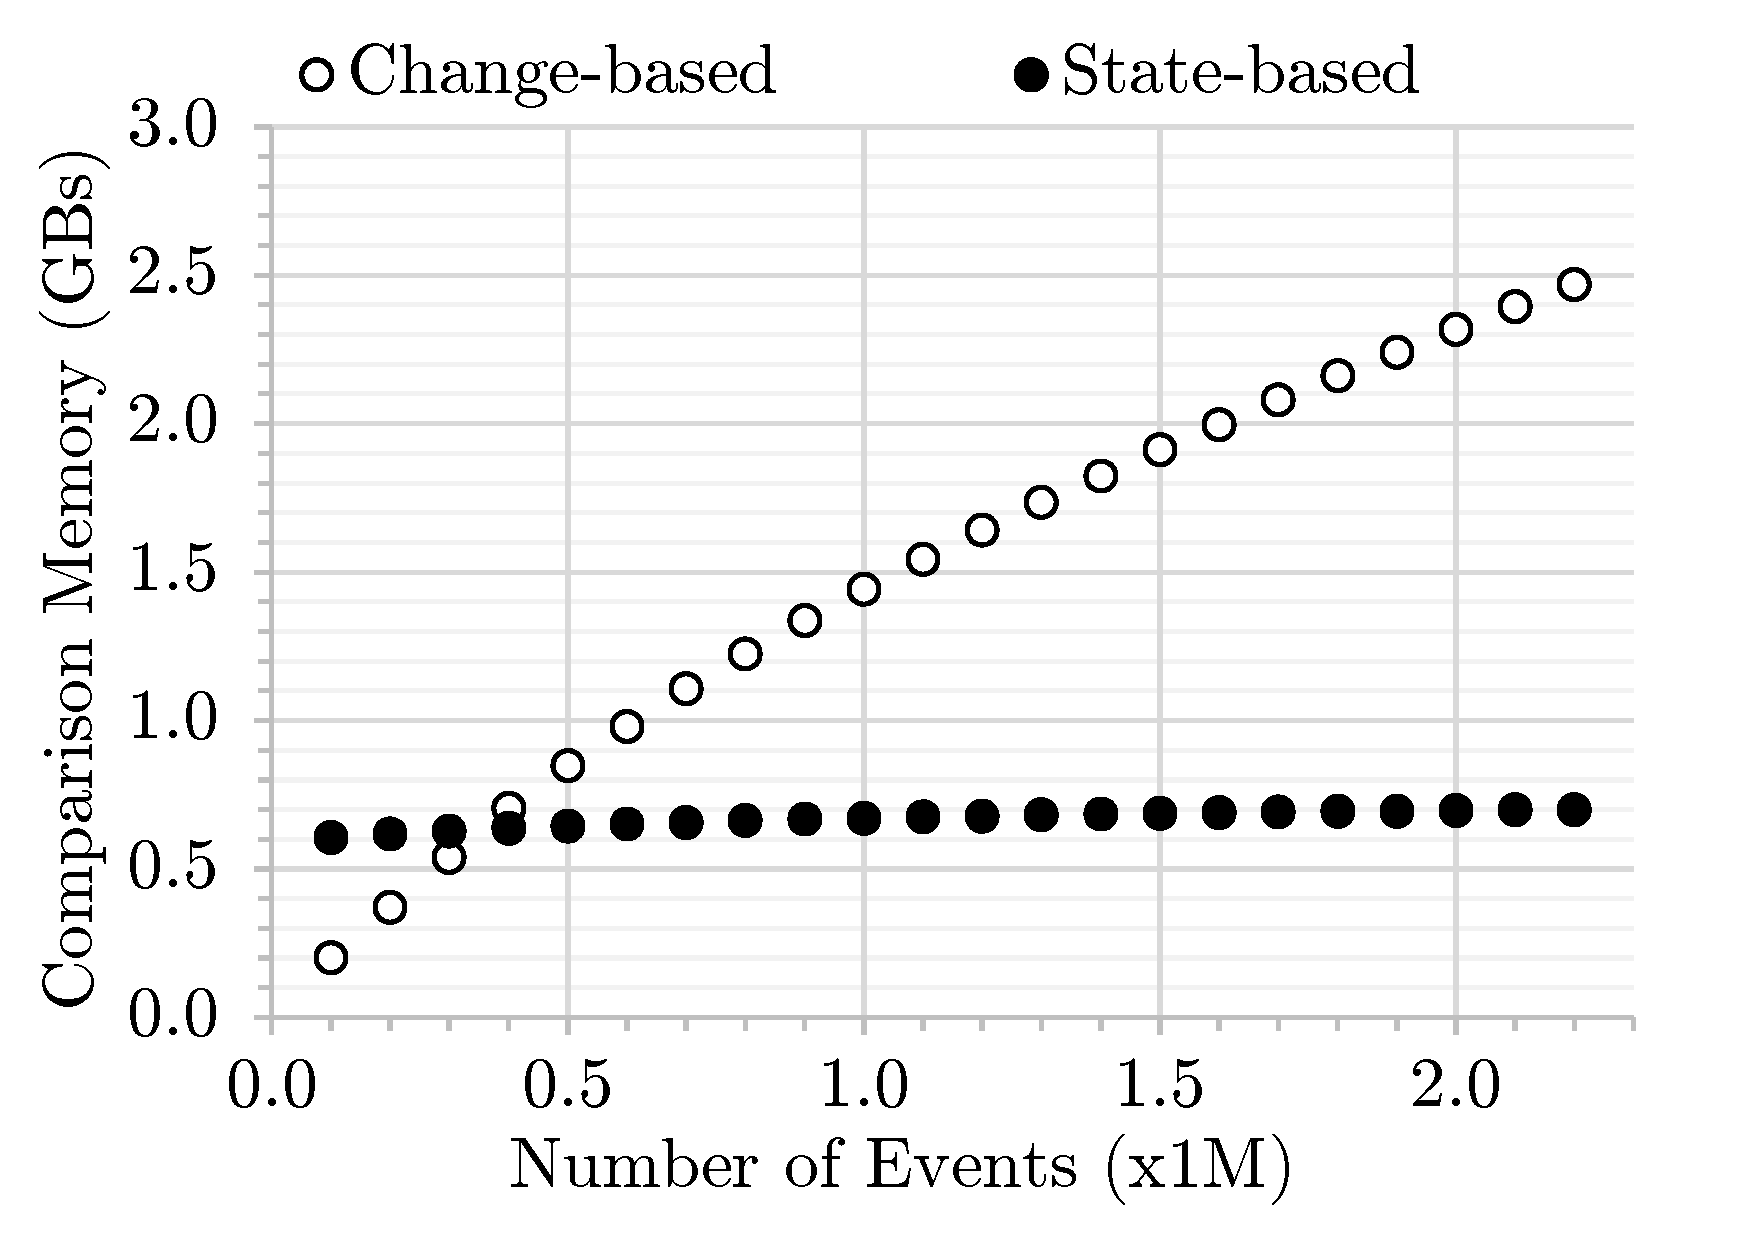
\includegraphics[width=\linewidth]{change-memory-events}
        \caption{change-only}
        \label{fig:change-memory-events}
    \end{subfigure}
    \caption{Memory footprint for homogeneous operations.}
    \label{fig:operation_memory_events}
\end{figure}

Figures \ref{fig:operation_time_events} and \ref{fig:operation_memory_events} exhibit the comparison time and memory footprint of models that have been modified using homogeneous operations -- \textsf{add}, \textsf{remove}, \textsf{move}, or \textsf{set} only. We can notice that in all figures change-based comparison outperforms its state-based counterpart, particularly when the number of change events is small relative to the size of the model. As the number of modifications grows, eventually change-based comparison becomes slower than state-based comparison. In our experiments, this happens when the number of events is greater than 4 million (Figure \ref{fig:add-time-events}). Change-based comparison also becomes slower when the size of models shrinks (due to a large number of delete events) as depicted in Figure \ref{fig:delete-memory-events} as the change-based comparison still needs to load these change events and construct its element tree; in contrast, deletion means less work for state-based comparison. In terms of memory footprint, change-based comparison only performs better than state-based comparison when the number of change events is less than 0.3 millions as depicted in Figure \ref{fig:operation_memory_events}.

\section{Conclusions}
\label{sec:conclusions_6}
This chapter has proposed an approach to identify differences between two versions of a model persisted in change-based format. It works by loading the recent changes, since a last shared version, of both versions into memory, constructing partial states of the versions based on the information in the latest changes, and using specific rules to identify differences between the versions' elements and features.   

Based on the evaluation results, this study argues that the change-based comparison approach works at its best for large models that have been modified a moderate number of times. Models that have been excessively modified and experience a significant reduction on model size could impair the performance of change-based comparison as a high number of change records have to be read and loaded into memory.

This chapter has addressed the second research question of this study, \textbf{In a changed-based format, how can differences between models be identified, and how does change-based model differencing perform, in terms of speed and memory footprint, compared to state-based model differencing?} (RQ2). Change-based persistence can be used to identify differences between two versions of a model. The change-based representation of the two versions contains all the necessary information to identify elements that have been modified since their last shared version. In this way, we can localise the model differencing only to the elements that have been recently modified. In other words, not all elements are necessary to be inspected, matched, and diffed. We can use the information to reconstruct the partial states of the two versions and then compare their elements and features using specific rules to identify their differences.  

The change-based model differencing proposed in this research consists of three phases: event loading, element tree construction, and diff computation. In the event loading phase, the implementation loads change events recorded in two change-based model persistence files into memory starting from the line their change events are different. The information that the loaded change events contains are used to construct an element three. An element three essentially is the partial states -- only the affected elements and features -- of the two versions being compared including the shared original version. It is possible since change events are designed to contain adequate information to construct the element three. A diff computation is then executed to identify the differences using a set of predefined rules (i.e., if an element is created in one of the versions it means that the element does not exist in the other version as well as in the original version).

The evaluation results suggest that the the proposed change-based model differencing executes faster than traditional, state-based model differencing.
However, the change-based model differencing needs to load change events from a change-based persistence into main memory and thus may requires more memory than for state-based state-based model differencing. In our evaluation, this occurs when the number of change events exceeds 400,000. Arguably, diff and merge operations are usually performed on smaller deltas than this work's evaluation.

%Differencing of large models can be time-consuming since every element has to be inspected, matched, and compared with its respective element in other models. This can result in bottlenecks in collaborative modelling environments, where identifying differences between two versions of a model is desirable. Reducing the comparison process to only the elements that have been modified since a previous known state (e.g., previous version) could significantly reduce the time required for large model differencing. 
%
%This Chapter presents how change-based model persistence can be used to localise the differencing of models so that only elements affected by recent changes are compared and to substantially reduce differencing time (up to 90\% in some experiments) compared to state-based model differencing. 
%
%Based on the findings, we argue that the change-based comparison approach works at its best for large models that have been modified a moderate number of times. Models that have been excessively modified and experience significant reduction on model size could impair the performance of change-based comparison as a great number of change records have to be read and loaded into memory. 

\chapter{Efficient Conflict Detection of Change-based Models}
\label{ch:conflict_detection}
  
In Chapter \ref{ch:model_differencing}, this work have demonstrated that  change-based model persistence can be exploited to speed up model differencing. In this Chapter, this work extends the proposed approach in Chapter \ref{ch:model_differencing} also by leveraging change-based model persistence to improve the performance of conflict detection in model versioning. The proposed approach can substantially reduce conflict detection time (up to 90\% in some experiments) compared to state-based model differencing. 

\section{Introduction}
\label{sec:introduction_7}
State- and change-based model conflict detection have been discussed briefly in Sections \ref{sec:emfcompare_conflict_detection} and \ref{sec:emfstore_conflict_detection}. The state-based approach, represented by EMF Compare \cite{emfcompare2018developer}, does come with drawbacks. First, it cannot detect conflicts as accurate as change-based approach can as their changes are derived -- not the real historical changes. Second, EMF Compare uses 3-way model comparison \cite{emfcompare2018developer} thus hypothetically its conflict detection should perform relatively slower than the change-based approach, since it has to perform state-based model differencing twice to derive changes events: changes events between left and original versions, and change events between right and original versions. 

Change-based model conflict detection \cite{koegel2010operation}, represented by EMF Store \cite{emfstore2019what}, also has drawbacks. EMF Store purely works on comparing change events and detects conflicts based on predefined rules; it does not consider the eventual states of two versions that are being compared. Thus, two change events that modifies a same feature are considered in conflict even though both change events produce the same eventual states. This condition can lead EMF Store to oversensitive conflict detection. In terms of performance, as has been presented in Chapter \ref{ch:model_differencing}, the change-based approach is faster than its state-based counterparts in model differencing. Thus, it is expected that it can also performs better that the state-based approach in detecting conflicts.
 
In this Chapter, this work proposes a change-based model conflict detection that also considers the eventual states of modified elements. Thus, the performance and accuracy of model conflict detection can be improved, compared to state-based approach, without being oversensitive.
 
\section{Epsilon Change-based Model Conflict Detection}
\label{epsilon_change_based_model_conflict_detection}
The model conflict detection proposed in this study basically performs similar procedure to the phases of change-based model differencing discussed in Chapter \ref{sec:change_based_approach_for_comparing_models} except that (1) it only executes event loading and element tree construction phases and replaces diff computation phase with conflict computation phase, and (2) during element tree construction, it maps change events to the elements, features, and values that they modify. The change event mapping and conflict computation are discussed in the following Sections.

\subsection{Change Event Mapping}
\label{sec:change_event_mapping}
Using the information contained in change-based model persistence in Listings \ref{lst:cbp_right} and \ref{lst:cbp_left}, we can construct an element tree as depicted in Figure \ref{fig:right_element_tree_diagram} using the construction method presented in Section \ref{sec:tree_construction}. During the the construction, change events in Listings \ref{lst:cbp_right} and \ref{lst:cbp_left} are mapped to the affected elements, features, and values which act as the keys of the mapping. This registration forms many-to-many relationships between the keys and change events. In detail, the keys are \textsf{element} for elements, or a combination of \textsf{element-feature} for single-valued features or \textsf{element-feature-value} for multivalued-features. With this mapping, we can trace all events that affects certain elements, features, and values. The mapping of the events in Listings \ref{lst:cbp_right} and \ref{lst:cbp_left} is in Table \ref{tab:keyeventsmap}.

\begin{table}[ht]
\centering
\caption{The mapping of elements, features, and values in Figure \ref{fig:right_element_tree_diagram} to the events that affect them.}
\label{tab:keyeventsmap}
\begin{scriptsize}
\begin{sffamily}
\begin{tabular}{|m{0.25\linewidth}|m{0.26\linewidth}|m{0.26\linewidth}|}
\hline
\textbf{Key} & \textbf{Left Events} & \textbf{Right Events} \\ \hline
character                          & cl32, cl34                                & cr37, cr39                                 \\ \hline
character.name                     & cl34                                      & cr39                                       \\ \hline
attack                             & cl37                                      & cr31                                       \\ \hline
attack.parameters.target           & cl37                                      & cr31                                       \\ \hline
target                             & cl37                                      & cr31                                       \\ \hline
trcll                              & cl33, cl35                                & cr38, cr40                                 \\ \hline
trcll.name                         & cl43                                      & cr42                                       \\ \hline
trcll.generalizaticn               & cl33, cl35                                & cr38, cr40                                 \\ \hline
giant                              & cl39, cl40, cl41, cl42                    & cr33, cr34                                 \\ \hline
giant.name                         & cl40                                      &                                            \\ \hline
giant.cperaticns.cast              & cl39                                      & cr34                                       \\ \hline
giant.cperaticns.smash             &                                           & cr33                                       \\ \hline
knight                             & cl36                                      & cr32                                       \\ \hline
knight.generalizaticn              & cl36                                      &                                            \\ \hline
knight.cperaticns.smash            &                                           & cr32                                       \\ \hline
mage                               &                                           & cr35, cr41                                 \\ \hline
mage.generalizaticn                &                                           & cr41                                       \\ \hline
mage.cperaticns.cast               &                                           & cr35                                       \\ \hline
leftGen                            & cl31, cl32, cl33, cl35, cl36              &                                            \\ \hline
leftGen.general                    & cl32                                      &                                            \\ \hline
rightGen                           &                                           & cr36, cr37, cr38, cr40, cr41               \\ \hline
rightGen.general                   &                                           & cr37                                       \\ \hline
smash                              &                                           & cr32, cr33                                 \\ \hline
cast                               & cl38, cl39, cl40                          & cr34, cr35                                 \\ \hline
cast.name                          & cl38                                      &                                            \\ \hline
\end{tabular}\\
\end{sffamily}
c: change event; l: left side; r: right side; n: line number in change-based model persistence
\end{scriptsize}
\end{table}

\subsection{Theoretical Foundation} 
\label{sec:theoretical_foundation}
In the proposed conflict detection, we take two strategies from both change and state-based conflict detections to improve the accuracy of our approach. 
First, we exploit change events to accurately address real historical changes -- not derived ones -- of models. Second, we also take into account the original and eventual states of the modified models. Two sequences of change events that produce two eventual states that are equal to an original state are not treated as in conflict. The original and eventual states are already calculated during the construction of the \textsf{element tree} so that we do not to calculate them again in the conflict computation phases. Since all change events are also recorded to every element, feature, and value that they affected, we can retrieve all related change events that produce the eventual state of an element or feature. 

Let's say that we have the original state of an element $e_{o}$. We also have a set of change events $C_{L}$ = $\{$$c_{l1}$, $c_{l2}$, ..., $c_{lg}$$\}$ that we apply to $e_{o}$ that changes its state to element $e_{l}$ and $g = |C_{L}|$. 
\begin{equation} \label{eq:ecbp_left}
e_{o} + c_{l1} + c_{l2} + ... + c_{lg} \rightarrow e_{l}
\end{equation} 
We also have another set of change events $C_{R}$ = $\{$$c_{r1}$, $c_{r2}$, ..., $c_{rh}$$\}$ that we apply to $e_{o}$ that produces element $e_{r}$ and $h = |C_{R}|$.
\begin{equation} \label{eq:ecbp_right}
e_{o} + c_{r1} + c_{r2} + ... + c_{rh} \rightarrow e_{r}
\end{equation} 
\textbf{Non-conflict}. Instead of calculating conflict between change events, we start by checking the equivalency of the left and right states of an element to its original state. If the states of both sides are equivalent to the original state, regardless of how many change events have been applied, we can infer that there is no conflict between the members of the two change event sets, $C_{L}$ and $C_{R}$, since there is no change of eventual states. We also identify no conflict if an element is only modified on one side -- no change events applied on the other side.
\begin{equation} \label{eq:ecbp_nonconflict}
\begin{split}
& (e_{o} \equiv e_{l} \wedge e_{o} \equiv e_{r}) \vee |C_{L}| = 0 \vee |C_{R}| = 0 \Rightarrow\\
& \neg(\forall c_{l} \;!\; \forall c_{r}) \;|\; c_{l} \in C_{L}, c_{r} \in C_{R}
\end{split}
\end{equation} 
\textbf{Conflict}. A conflict occurs when one or both states, $e_{l}$ or/and $e_{r}$, are not equivalent to the original state $e_{o}$, and, at least, there is a change event applied on each side of the element; we can conclude that change event set $C_{L}$ is in conflict with the change event set $C_{R}$.
\begin{equation} \label{eq:ecbp_conflict}
\begin{split}
& (e_{o} \not\equiv e_{l} \vee e_{o} \not\equiv e_{r}) \wedge (|C_{L}| > 0 \wedge |C_{R}| > 0) \Rightarrow\\
& \forall c_{l} \;!\; \forall c_{r} \;|\; c_{l} \in C_{L}, c_{r} \in C_{R}
\end{split}
\end{equation} 
\textbf{Pseudo-conflict}. As in EMF Compare, we also implement pseudo conflict. Pseudo conflict is a conflict where $e_{l}$ and $e_{r}$ are equivalent or one of them is equivalent to $e_{o}$ thus they can be automatically resolved in conflict resolution without user intervention.
\begin{equation} \label{eq:ecbp_pseudoconflict}
\begin{split}
(& e_{o} \equiv e_{l} \vee e_{o} \equiv e_{r} \vee e_{l} \equiv e_{r}) \wedge (|C_{L}| > 0 \wedge |C_{R}| > 0)\\
& \Rightarrow \forall c_{l} \;!_{p}\; \forall c_{r} \;|\; c_{l} \in C_{L}, c_{r} \in C_{R}
\end{split}
\end{equation} 

Figure \ref{fig:conflict_states} are some examples how conflict and non-conflict change events are detected in the proposed approach (dashed arrow = left change event, solid arrow = right change events, circle = state). Figure \ref{fig:statechart_01} shows the initial state of an element is `a'. In the figure, the element has not been modified. Thus, no conflict is detected according to (\ref{eq:ecbp_nonconflict}). In Figure \ref{fig:statechart_02}, the element is modified on the right side (version) only. Thus, using (\ref{eq:ecbp_nonconflict}), no conflict is detected. In the figure, the state of the element is altered from `a' to `b' by change event $cr1$, and then altered again to `c' by change event $cr2$. In Figure \ref{fig:statechart_03}, even though an element has been modified on both sides, using (\ref{eq:ecbp_nonconflict}), no conflict is detected, since both left and right states are equal to the original state after the modification. In the figure, both $C_{L}$ and $C_{R}$ produces eventual states that are equal to the original state, `a'. 

\begin{figure}[ht]
    \begin{subfigure}[t]{0.30\linewidth}
        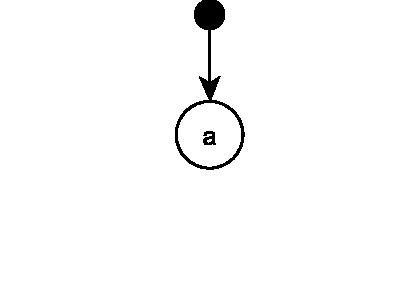
\includegraphics[width=\linewidth]{statechart_01}
        \caption{non-conflict}
        \label{fig:statechart_01}
    \end{subfigure}
    \hfill
    \begin{subfigure}[t]{0.30\linewidth}
        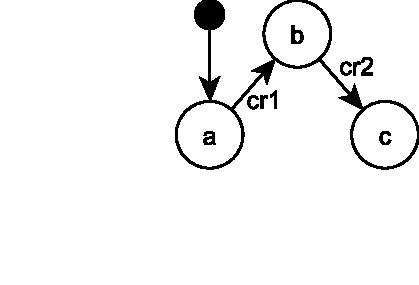
\includegraphics[width=\linewidth]{statechart_02}
        \caption{non-conflict}
        \label{fig:statechart_02}
    \end{subfigure}
    \hfill
    \begin{subfigure}[t]{0.30\linewidth}
        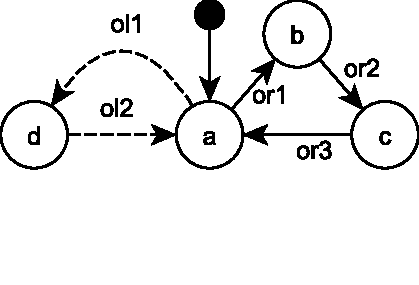
\includegraphics[width=\linewidth]{statechart_03}
        \caption{non-conflict}
        \label{fig:statechart_03}
    \end{subfigure}
    \\
    \begin{subfigure}[t]{0.30\linewidth}
        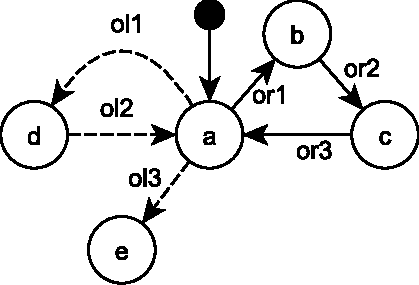
\includegraphics[width=\linewidth]{statechart_04}
        \caption{pseudo-conflict}
        \label{fig:statechart_04}
    \end{subfigure}
    \hfill
    \begin{subfigure}[t]{0.30\linewidth}
        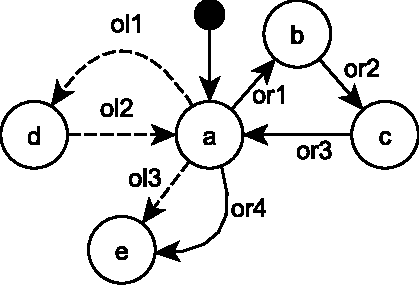
\includegraphics[width=\linewidth]{statechart_05}
        \caption{pseudo-conflict}
        \label{fig:statechart_05}
    \end{subfigure}
    \hfill
    \begin{subfigure}[t]{0.30\linewidth}
        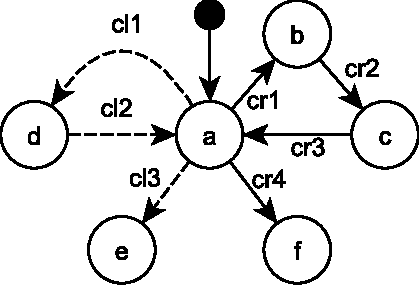
\includegraphics[width=\linewidth]{statechart_06}
        \caption{conflict}
        \label{fig:statechart_06}
    \end{subfigure}
    \caption{Conflicting and non-conflicting change events (dashed arrow = left change event, solid arrow = right change events, circle = state).}
    \label{fig:conflict_states}
\end{figure}

Using (\ref{eq:ecbp_pseudoconflict}), condition in Figure \ref{fig:statechart_04} can be detected as a \textsf{PSEUDO} conflict. \textsf{PSEUDO} conflict means that a conflict can be automatically resolved. This means that we can automatically select one of the two conflicting change event sets as the applied change events without needing for human intervention. Since $C_{R}$ produces the eventual state that is equal to the original state, that is `a'; it does not have any effect -- the changes are not intended or cancelled. Thus, all its change events can be automatically negated. In other words, only change events in $C_{L}$ that are accepted to produce the eventual state, which is `e'. Also using (\ref{eq:ecbp_pseudoconflict}), condition is \ref{fig:statechart_05} can also be detected as another \textsf{PSEUDO} conflict. Both change event sets, $C_{L}$ and $C_{R}$, produce the same eventual state, `e', that is different from the original state, `a'. This condition ca be automatically resolved since selecting one of the sets produces the same outcome. With (\ref{eq:ecbp_conflict}), the condition in Figure \ref{fig:statechart_06} can be detected as a \textsf{REAL} conflict since change event sets, $C_{L}$ and $C_{R}$, produces two different eventual states. The conflict cannot be automatically resolved and requires user intervention to choose which one is the desired eventual state, `e' or `f', and then the appropriate change event set should be selected to produce the eventual state.


\subsection{Conflict Computation} 
\label{sec:conflict_computation} 
We perform procedure in Algorithm \ref{alg:conflict_detection} and employ (\ref{eq:ecbp_conflict}) and (\ref{eq:ecbp_pseudoconflict}) inside it to identify conflicts between two CBPs. Basically, the algorithm works by iterating through all the elements, features, and values in the element three (Figure \ref{fig:right_element_tree_diagram}) and checking the equivalency of their original and eventual states as well the numbers of change events applied to them. The results are then used as inputs to decide whether a conflict has been detected or not.

\begin{table*}[ht]
  \centering
  \caption{Conflicting change events in Listings \ref{lst:cbp_right} and \ref{lst:cbp_left} identified using the proposed conflict detection.}
  \label{table:conflicts_cbp}
  \begin{scriptsize}
    \begin{tabular}{|p{0.04\linewidth}|p{0.38\linewidth}|p{0.38\linewidth}|
        p{0.07\linewidth}|}
      \hline
      \textbf{ID} & 
      \textbf{Left Change Events (Bob)} & 
      \textbf{Right Change Events (Alice)} & 
      \textbf{Type}\\ 
      \hline
      CB1 & 
      set troll.name from "Troll" to "Ogre" & 
      set troll.name from "Troll" to "Orc" & 
      real \\
      \hline
      CB2 & move target in character.parameters from 1 to 2 & 
      move target in character.parameters from 1 to 0 & 
      real \\ 
      \hline
      CB3 & 
      \begin{minipage}[t]{\linewidth}
        \raggedright
        \begin{itemize}[leftmargin=0pt]
          \setlength
          \item[] unset cast.name from "cast" to null
          \item[] remove cast from giant.operations at 0
          \item[] delete cast type Operation
          \item[] unset giant.name from "Giant" to null
          \item[] delete giant
        \end{itemize}
      \end{minipage}
      & 
      \begin{minipage}[t]{\linewidth}
        \raggedright
        \begin{itemize}[leftmargin=0pt]
          \setlength
          \item[] remove cast from giant.operations at 0
          \item[] add cast to mage.operations at 0
          \item[] remove smash from knight.operations at 0
          \item[] add smash to giant.operations at 1
        \end{itemize}
      \end{minipage}
      & 
      real, dependency\\ 
      \hline
      CB4 & 
      set character.name from "Character" to "Hero" & 
      set character.name from "Character" to "Hero" & 
      pseudo\\ 
      \hline
    \end{tabular}
  \end{scriptsize}
\end{table*}

%------------------------------------------------------------------------------

\IncMargin{1.5em}
\begin{algorithm}[]
  \begin{scriptsize}
    \SetKwInOut{Input}{input}
    \SetKwInOut{Output}{output}
    \Input{an instance of ElementTree $elementTree$}
    \Begin{
      $conflictList$ $\leftarrow$ ConflictList()\;
      \ForEach{$element$ \In $elementTree$}{
        \tcp{Handle conflicts with deletion ----------------------------}
        \If{isLeftDeleted($element$) \Or isRightDeleted($element$)}{
          $leftEvents$ $\leftarrow$ getAllRelatedLeftEvents($element$)\;
          $rightEvents$ $\leftarrow$ getAllRelatedRightEvents($element$)\;
          \If{size($leftEvents$) > 0 \AndA size($rightEvents$) > 0}{
            $conflict$ $\leftarrow$ createConflict($leftEvents$, $rightEvents$)\;
            \If{isLeftDeleted($element$) \AndA isRightDeleted($element$)}{
              setPseudo($conflict$)\;
            }
            addConflict($conflict$, $conflictList$)\;
          }
        }
        \tcp{Handle conflicts with cross-container move --------------------------}
        \If{(getOriginalContainer($element$) <> getLeftContainer($element$) \Or getOriginalContainingFeature($element$) <> getLeftContainingFeature($element$)) \Or
          (getOriginalContainer($element$) <> getRightContainer($element$) \Or getOriginalContainingFeature($element$) <> getRightContainingFeature($element$))}{
          $leftEvents$ $\leftarrow$ getAllRelatedLeftEvents($element$)\;
          $rightEvents$ $\leftarrow$ getAllRelatedRightEvents($element$)\;
          \If{size($leftEvents$) > 0 \AndA size($rightEvents$) > 0}{
            $conflict$ $\leftarrow$ createConflict($leftEvents$, $rightEvents$)\;
            \If{getLeftContainer($element$) = getRightContainer($element$) \AndA getLeftContainingFeature($element$) = getRightContainingFeature($element$}{
              setPseudo($conflict$)\;
            }
            addConflict($conflict$, $conflictList$)\;
          }
        }
        \ForEach{$feature$ \In getFeatures($element$)}{
          \tcp{Handle single-valued feature --------------------------}
          handleSingleValuedFeature($element$, $feature$, $conflictList$)\;\label{line:conflict_single_value}
          \tcp{Handle multi-valued feature --------------------------} 
          handleMultiValuedFeature($element$, $feature$, $conflictList$)\;\label{line:conflict_multi_value}
        }
      }
      \Return{$conflictList$}\;
    }
  \end{scriptsize}
  \caption{Algorithm for conflict detection using element tree.}
  \label{alg:conflict_detection}
\end{algorithm}
\DecMargin{1.5em}

The algorithm starts by creating a empty list \textsf{conflictList} to contain identified conflicts at lines 2. The algorithm then iterates through all the elements, features, and values in the element three. 

\subsubsection{Conflict with Deletion} 
\label{sec:delete_conflict} 
At lines 4 to 11 in Algorithm \ref{alg:conflict_detection}, the algorithm checks if there is a conflict related to a deletion of an element.
If an element is deleted on one side or both sides, it means that all events related to the element on both sides should be in conflict. 
To get all the related events, the algorithm use functions \textsf{getAllRelatedLeftEvents($element$)} 
and \textsf{getAllRelatedLeftEvents($element$)} (the element acts as a map key to access the change events) that return two sets of the related events, 
\textsf{leftEvents} and \textsf{rightEvents} respectively. The related events are events applied to the deleted element, including its sub-elements and features, 
and events that are parts of composite events. If both sets of events are not empty then a conflict is created containing both sets of events. 
If the element is deleted on both sides then we set the conflict as \textsf{PSEUDO}. The identified conflict is then added to \textsf{conflictList}.

\IncMargin{1.5em}
\begin{algorithm}[]
  \begin{scriptsize}
    \SetKwInOut{Input}{input}
    \SetKwInOut{Output}{output}
    \Input{an element $element$}
    \Input{a feature $feature$}
    \Input{a list to contain conflicts $conflictList$}
    \Begin{
      \tcp{Handle single-valued feature --------------------------}
      \If{isSingleValued($feature$)}{
        $originalValue$ $\leftarrow$ getOriginalValue($feature$)\;
        $leftValue$ $\leftarrow$ getLeftValue($feature$)\;
        $rightValue$ $\leftarrow$ getRightValue($feature$)\;
        $leftEvents$ $\leftarrow$ getAllRelatedLeftEvents($element$, $feature$)\;
        $rightEvents$ $\leftarrow$ getAllRelatedRightEvents($element$, $feature$)\;
        \If{$originalValue$ <> $leftValue$ \Or $originalValue$ <> $rightValue$ \AndA size($leftEvents$) > 0 \AndA size($rightEvents$) > 0}{
          $conflict$ $\leftarrow$ createConflict($leftEvents$, $rightEvents$)\;
          \If{ $leftValue$ = $rightValue$}{
            setPseudo($conflict$)\;
          }
          addConflict($conflict$, $conflictList$)\;
        }
      }
    }
  \end{scriptsize}
  \caption{Algorithm to handle single-valued feature in conflict detection using element tree -- handleSingleValuedFeature($element$, $feature$, $conflictList$) at line 27 in Algorithm \ref{alg:conflict_detection}.}
  \label{alg:conflict_single_valued_feature}
\end{algorithm}
\DecMargin{1.5em}

As an example, when the iteration reach element \textsf{giant} in Figure \ref{fig:right_element_tree_diagram}, the algorithm identifies that the element has been deleted only on the left side.
The algorithm then collects all the related events from both sides of the element. 
The left events are all events parts of the composite event that deletes the element. 
The right events consist of events that move operation \textsf{smash} from class \textsf{knight} to class \textsf{giant} and events that
move operation \textsf{cast} from class \textsf{giant} to class \textsf{mage}. The algorithm then creates a conflict that consists of these events 
producing conflict \textsf{CB3} in Table \ref{table:conflicts_cbp}. The conflict is not set \textsf{PSEUDO} since, besides deleted on the left side, its feature also has been modified on the right side. 

\subsubsection{Conflict between Cross-container Moves} 
\label{sec:move_conflict} 
Lines 15 to 25 in Algorithm \ref{alg:conflict_detection} are dedicated to identify conflicts related to cross-container moves. 
First, the algorithm checks if an element has been moved from its original container to another container, on one of the sides or both sides. 
If only on one side or both sides the element has been moved to another container, 
it continues to check the number of events related to the element by firstly obtaining change events related to the element on 
both sides using functions \textsf{getAllRelatedLeftEvents($element$)} and \textsf{getAllRelatedLeftEvents($element$)} yielding two sets of events, 
\textsf{leftEvents} and \textsf{rightEvents}. If the element has, at least, one event on each side,
a conflict is created containing \textsf{leftEvents} and \textsf{rightEvents}. 
If on both sides the element is moved to a same container or the element is moved but finally returns to its original container on one of its sides then the conflict is set to \textsf{PSEUDO}. The conflict is then added to \textsf{conflictList}. 

\subsubsection{Single-valued Feature Conflict} 
\label{sec:single_valued_conflict}
Conflicts that involve single-valued features are handled by the procedure at line \ref{line:conflict_single_value} in Algorithm \ref{alg:conflict_detection}, which is elaborated in Algorithm \ref{alg:conflict_single_valued_feature}. The procedure starts by retrieving \textsf{leftValue}, \textsf{rightValue}, and \textsf{originalValue} of a single-valued feature. It then checks the inequality of \textsf{leftValue} and \textsf{rightValue} to \textsf{originalValue}. If one of \textsf{leftValue} and \textsf{rightValue} are not equal to \textsf{originalValue}, it then continues to check the number of change events related to the feature by firstly retrieving them using functions \textsf{getAllRelatedEvents($element$, $feature$)} and \textsf{getAllRelatedRightEvents($element$, $feature$)} (element and feature act as a map key to access the events) yielding two sets of related events, \textsf{leftEvents} and \textsf{rightEvents}. If \textsf{leftEvents} and \textsf{rightEvents} are not empty then a conflict that contains these events is instantiated. The procedure then checks the equality of \textsf{leftValue} and \textsf{rightValue} and set the conflict to \textsf{PSEUDO} if \textsf{leftValue} and \textsf{rightValue} are equal or one of them is equal to \textsf{originalValue}. Finally, the conflict is put into \textsf{conflictList}. 

\IncMargin{1.5em}
\begin{algorithm}[]
  \begin{scriptsize}
    \SetKwInOut{Input}{input}
    \SetKwInOut{Output}{output}
    \Input{an element $element$}
    \Input{a feature $feature$}
    \Input{a list to contain conflicts $conflictList$}
    \Begin{
      \tcp{Handle multi-valued feature --------------------------}
      \If{isMultiValued($feature$)}{
        \uIf{isOrdered($feature$)}{
          $values$ $\leftarrow$ getUnequalLeftAndRightValues($feature$)\;
          \ForEach{$value$ \In $values$}{
            $leftEvents$ $\leftarrow$ getAllRelatedLeftEvents($element$, $feature$, $value$)\;
            $rightEvents$ $\leftarrow$ getAllRelatedRightEvents($element$, $feature$, $value$)\;
            \If{size($leftEvents$) > 0 \AndA size($rightEvents$) > 0}{
              $conflict$ $\leftarrow$ createConflict($leftEvents$, $rightEvents$)\;
              \If{getLeftIndex($value$, $feature$) = getRightIndex($rightValue$, $feature$)}{
                setPseudo($conflict$)\;
              }
              addConflict($conflict$, $conflictList$)\;
            }       
          }
        }\ElseIf{\Not isOrdered($feature$)}{
          $values$ $\leftarrow$ getXORLeftAndRightValues($feature$)\;
          \ForEach{$value$ \In $values$}{
            $leftEvents$ $\leftarrow$ getAllRelatedLeftEvents($element$, $feature$, $value$)\;
            $rightEvents$ $\leftarrow$ getAllRelatedRightEvents($element$, $feature$, $value$)\;
            \If{size($leftEvents$) > 0 \AndA size($rightEvents$) > 0}{
              $conflict$ $\leftarrow$ createConflict($leftEvents$, $rightEvents$)\;
              \If{isExisted($value$, $feature$) = isExisted($rightValue$, $feature$)}{
                setPseudo($conflict$)\;
              }
              addConflict($conflict$, $conflictList$)\;
            }       
          }
        }
      }
    }
  \end{scriptsize}
  \caption{Algorithm to handle multi-valued feature in conflict detection using element tree -- handleMultiValuedFeature($element$, $feature$, $conflictList$) at line 28 in Algorithm \ref{alg:conflict_detection}.}
  \label{alg:conflict_multi_valued_feature}
\end{algorithm}
\DecMargin{1.5em}

For example, when the iteration reach feature \textsf{name} of class \textsf{troll}, the algorithm retrieves the left, right, and original values of the feature, yielding ``Ogre'', ``Orc'', and ``Troll'' respectively. Since ``Ogre'' and Orc'' are not equal to ``Troll'', the algorithm continues to retrieve two sets of events related to the feature. Only one event contained exists in each set. On the left side, the event sets the name of class \textsf{troll} from ``Troll'' to ``Ogre'', while on the right side, the the event sets it from ``Troll'' to ``Orc''. Both event sets are not empty thus a conflict containing them is created. Since ``Ogre'' is not equal to ``Orc'' the conflict is not set to \textsf{PSEUDO}. This conflict is the conflict \textsf{CB1} in Table \ref{table:conflicts_cbp}. This part of the algorithm also identifies conflict \textsf{CB4} except that this conflict is set to \textsf{PSEUDO} since both sides change class \textsf{character}'s \text{name} to ``Hero''.   

\subsubsection{Ordered Multi-valued Feature Conflict} 
\label{sec:ordered_conflict}
Conflicts that involve multi-valued features are handled by the procedure at line \ref{line:conflict_multi_value} in Algorithm \ref{alg:conflict_detection}, which is elaborated in Algorithm \ref{alg:conflict_multi_valued_feature}, where ordered multi-valued features are addressed at lines 3-15. The procedure relies on function \textsf{getUnequalLeftAndRightValues}. The function returns all values from left and right sides that are not equal to their original states in terms of (in)existence and indexes. For example, in Figure \ref{fig:right_element_tree_diagram}, parameter \textsf{target} in feature \textsf{parameters} is at index 2 on the left side but at index 1 in its original state. Thus, the value is included in the returned set. On the right side, this parameter is also at different index to its original index but it is already included the returned set. 

The algorithm then iterates through the values of the set. For each value, it retrieves all events related to the value on this feature (element, feature, and value act as a map key to access the events) using functions \textsf{getAllRelated *Events($element$, $feature$, $value$)}, yielding two sets of events, \textsf{leftEvents} and \textsf{rightEvents}. If both sets of events are not empty then a conflict is created. If the value on both sides is at the same index then the conflict is \textsf{PSEUDO}. Lastly, the conflict is added to \textsf{conflictList}. The parameter \textsf{target} in feature \textsf{parameters} has been concurrently modified; it has one event on each side: parameter \textsf{target} is moved to the last index on the left side and to the first index on the right. Thus, a conflict in detected. This conflict is presented as conflict \textsf{CB2} in Table \ref{table:conflicts_cbp}.

%\begin{figure}[ht]
%    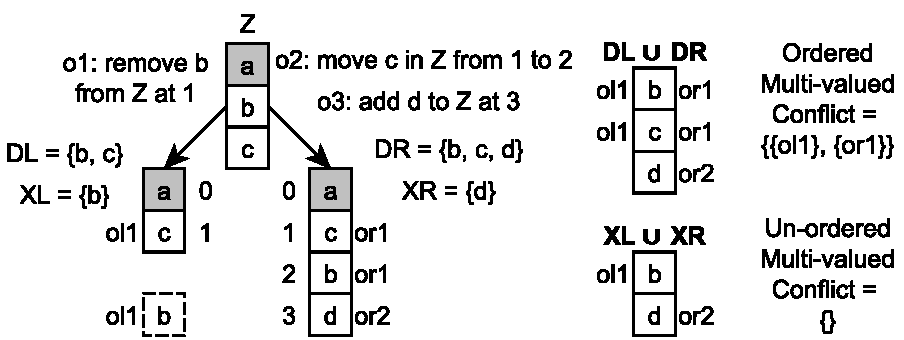
\includegraphics[width=\linewidth]{multi_valued_conflict_detection}
%    \caption{Detecting conflicts in Multi-valued features ($D$: values that are different at every index; $X$: XOR of values).}
%    \label{fig:multi_valued_conflict_detection}
%\end{figure}

\subsubsection{Unordered Multi-valued Feature Conflict} 
\label{sec:unordered_conflict}
Conflict detection for un-odered, multi-valued features is handled at lines 16 to 29 in Algorithm \ref{alg:conflict_multi_valued_feature}. Instead of using function \textsf{getUnequalLeftAndRightValues}, it employs function \textsf{getXORLeftAndRightValues}. The function also returns all values from left and right sides that are not equal to their original states but only in terms of (in)existence since indexing is not important in un-ordered features. The procedure to detect a conflict is similar to the procedure for ordered features. The difference is that, to determine if a conflict is \textsf{PSEUDO} or not, it checks the existence of values (function \textsf{isExisted}).

%\begin{figure*}
%    \begin{tabular}{l|c|r}
%        \begin{subfigure}[t]{0.31\linewidth}
%            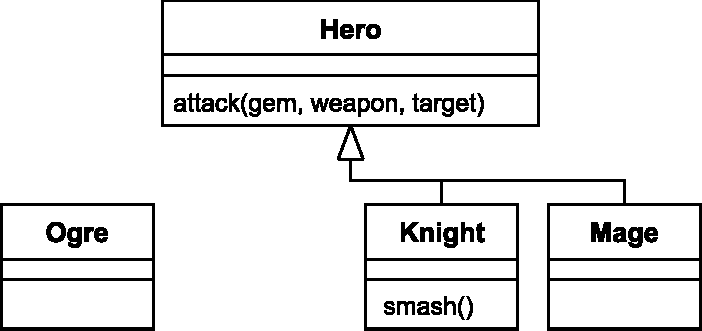
\includegraphics[width=\linewidth]{class_diagram_merged_ecbp}
%            \caption{Epsilon CBP}
%            \label{fig:class_diagram_merged_ecbp}
%        \end{subfigure}
%        &
%        \begin{subfigure}[t]{0.31\linewidth}
%            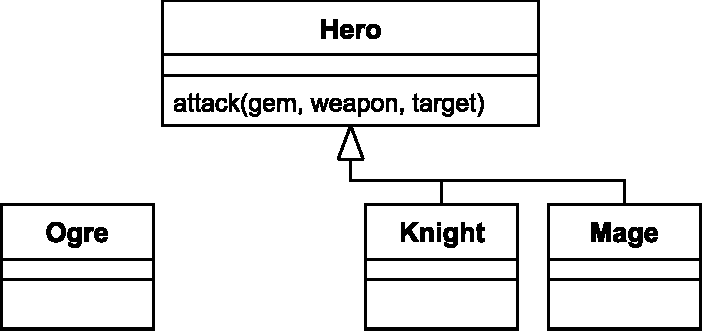
\includegraphics[width=\linewidth]{class_diagram_merged_emfc}
%            \caption{EMF Compare}
%            \label{fig:class_diagram_merged_emfc}
%        \end{subfigure}
%        &
%        \begin{subfigure}[t]{0.31\linewidth}
%            \includegraphics[width=\linewidth]{class_diagram_merged_emfs}
%            \caption{EMF Store}
%            \label{fig:class_diagram_merged_emfs}
%        \end{subfigure}
%    \end{tabular}
%    \caption{Merged models of models in Figure \ref{fig:class_diagram_rpg} after applying all-left-to-right merging.}
%    \label{fig:class_diagram_merged}
%\end{figure*}

%\section{Merging}
%\label{sec:merging}
%Conflict resolution and merging strategies are out of the scope of this paper. However, it is important to present the merged models of these three approaches in order inspect their correctness. Thus, we present the merged models of the models in Figure \ref{fig:class_diagram_rpg} using these three different approaches. The merge is all-left-to-right merge which means the left changes is prioritised above right changes. In other words, the right changes is applied first to the original model so that the left changes can override the right changes. If there is a conflict then the conflicting right changes are cancelled. In EMF Compare, this cancellation means only the left changes are executed, the right changes are \emph{not executed}, while, in Epsilon CBP and EMF Store, the right changes are \emph{reversed} so that the affected elements are brought back to their original states.    
%
%In the default implementation of EMF Compare, the all-left-to-right merge sets the right model as the target and the left model as the source. This means the left changes are not applied to the original model. Instead, they are applied to the right model. Using this strategy, if we resolve all the conflicts in Table \ref{table:conflicts_emfc} using the all-left-to-right merge, we get a merged model as in Figure \ref{fig:class_diagram_merged_emfc}. All the right events are not executed. Instead, in the right model, class \textsf{character}'s feature \text{name} is set to ``Hero'' and class \textsf{troll}'s feature \textsf{name} is set to ``Ogre''. Also, operation \textsf{cast} and class \textsf{giant} are removed from the right model. The removal of class \textsf{giant} also removes operation \textsf{smash} since the operation is contained by the class in the right model. 
%
%For Epsilon CBP and EMF Store, applying the all-left-to-right merging requires all the right events of the conflicts in Tables \ref{table:conflicts_emfs} and \ref{table:conflicts_cbp} to be reversed. This reversal brings back the states of the elements affected by the conflicting right events to their original states which makes the conflicting left events safe to be applied to the original model. All right events are applied first followed by the reversed conflicting right events and then by all left events (see Listings \ref{lst:cbp_merged_emfs} and \ref{lst:cbp_merged_ecbp}). In this order, the events are applied to the original model, not the right model as in the EMF Compare, to produce the merged model.
%
%\begin{lstlisting}[firstnumber=1,style=eol,caption={Merged change events of the models in Figure \ref{fig:class_diagram_rpg} and Listings \ref{lst:cbp_right} and \ref{lst:cbp_left} using EMF Store. The commented lines are added only to improve readability.},label=lst:cbp_merged_emfs]
%#--right events--
%move target in attack.parameters from 1 to 0
%remove smash from knight.operations at 0 composite l1
%add smash to giant.operations at 0 composite l1
%remove cast from giant.operations at 1 composite l2
%add cast to mage.operations at 0 composite l2
%create rightGen type Generalization
%set rightGen.general to character
%set troll.generalization to rightGen
%set character.name from "Character" to "Hero"
%remove rightGen from troll.generalization composite l3
%set mage.generalization to rightGen composite l3
%set troll.name from "Troll" to "Orc"
%#--reversed conflicting right events--
%set troll.name from "Orc" to "Troll"
%remove rightGen from mage.generalization composite l3r
%set troll.generalization to rightGen composite l3r
%set character.name from "Hero" to "Character"
%remove rightGen from troll.generalization
%set rightGen.general from character to null
%delete rightGen
%remove cast from mage.operations at 0 composite l2r
%add cast to giant.operations at 1 composite l2r
%remove smash from giant.operations at 0 composite l1r
%add smash to knight.operations at 0 composite l1r
%move target in attack.parameters from 0 to 1
%#--left events--
%create leftGen type Generalization
%set leftGen.general to character
%set troll.generalization to leftGen
%set character.name from "Character" to "Hero"
%remove leftGen from troll.generalization composite r1
%set knight.generalization to leftGen composite r1
%move target in attack.parameters from 1 to 2
%unset cast.name from "cast" to null composite r2
%remove cast from giant.operations at 0 composite r2
%delete cast composite r2
%unset giant.name from "Giant" to null composite r2
%delete giant comp r2
%set troll.name from "Troll" to "Ogre"
%\end{lstlisting}
%
%\vspace{-20pt}
%\begin{lstlisting}[firstnumber=1,style=eol,caption={Merged change events (operations) of the models in Figure \ref{fig:class_diagram_rpg} and Listings \ref{lst:cbp_right} and \ref{lst:cbp_left} using Epsilon CBP. The commented lines are added only to improve readability.},label=lst:cbp_merged_ecbp]
%#--right events--
%move target in attack.parameters from 1 to 0
%remove smash from knight.operations at 0 composite l1
%add smash to giant.operations at 0 composite l1
%remove cast from giant.operations at 1 composite l2
%add cast to mage.operations at 0 composite l2
%create rightGen type Generalization
%set rightGen.general to character
%set troll.generalization to rightGen
%set character.name from "Character" to "Hero"
%remove rightGen from troll.generalization composite l3
%set mage.generalization to rightGen composite l3
%set troll.name from "Troll" to "Orc"
%#--reversed conflicting right events--
%set troll.name from "Orc" to "Troll"
%remove cast from mage.operations at 0 composite l2r
%add cast to giant.operations at 1 composite l2r
%remove smash from giant.operations at 0 composite l1r
%add smash to knight.operations at 0 composite l1r
%move target in attack.parameters from 0 to 1
%#--left events--
%create leftGen type Generalization
%set leftGen.general to character
%set troll.generalization to leftGen
%set character.name from "Character" to "Hero"
%remove leftGen from troll.generalization composite r1
%set knight.generalization to leftGen composite r1
%move target in attack.parameters from 1 to 2
%unset cast.name from "cast" to null composite r2
%remove cast from giant.operations at 0 composite r2
%delete cast composite r2
%unset giant.name from "Giant" to null composite r2
%delete giant comp r2
%set troll.name from "Troll" to "Ogre"
%\end{lstlisting}
%
%The drawback of the EMF Compare approach is that it set the right model as the target for merging changes resulting the lost of operation \textsf{smash} in the merged model (Figure \ref{fig:class_diagram_merged_emfc}). In contrast, Epsilon CBP and EMF Store reverse the event that moves operation \textsf{smash} from class \textsf{knight} to class \textsf{giant} so that it moves back operation \textsf{smash} from class \textsf{giant} to class \textsf{knight}. The drawback of EMF Store is that it does not concern about the eventual states produced by the conflicting events. It only concern that a feature has been modified concurrently on both sides identified by the presence of, at least, an event on each side. For example, the eventual states of class \textsf{troll}'s feature \textsf{generalization} are \textsf{null} in the original, left, and right models. However, these are not considered by EMF Store. Instead, it only identifies that there are events on both sides associated to this feature. Thus, conflict \textsf{ES1} in \ref{table:conflicts_emfs} is generated. In consequence, all events related to the feature on the right side, and the events that are part of their composite events, are reversed resulting the exclusion of generalization \textsf{rightGen} from the merged model. This drawback has been addressed by the Epsilon CBP by checking the equality of the original, left, and right states of the feature. Since they are all equal then there is no conflict between the events. Thus, Epsilon CBP produces a merged model as in Figure \ref{fig:class_diagram_merged_ecbp}.


\section{Evaluation Method}
\label{sec:evaluation_conflict_Detection}
This section presents the method that was employed to evaluate the change-based conflict detection approach proposed in this study and discuss the results. In order to assess the performance benefits of the proposed conflict detection, this study has evaluated it against a mature and widely-used state-based model comparison tool, EMF Compare \cite{emfcompare2018developer,eclipse2017compare}, and another implementation of change-based model persistence, EMF Store \cite{koegel2010emfstore}. EMF Store is not included in the model differencing evaluation in Chapter \ref{ch:model_differencing} since it works purely on changes, and it is designed to identify conflict between changes; not for finding differences between models. 

Since there are no manually developed, large models persisted in the proposed change-based format yet, the dataset for this experiments was constructed from a large model reverse-engineered from the Eclipse Epsilon project \cite{eclipse2018epsilongit,eclipse2017epsilon}. This model conforms to the Java metamodel \cite{eclipse2018modiscojava} and consists of more than 1.6 million elements with a size of 224 MBs when persisted in XMI. 

The original model was cloned to produce two new (left and right) models and perform operations (\textsf{add}, \textsf{remove}, \textsf{move}, \textsf{set} with random elements, features, indexes, and values) on both models to create differences. In the evaluation, 1.1 million artificial changes were applied to each model, generating over 1.1 million events (one operation can generate more than one event, e.g. a \textsf{move} between features generates \textsf{remove} and \textsf{add} events). Events generated by the changes were persisted in the proposed change-based format (to be used later in change-based model comparison). After every 50,000 changes, a measurement point is made. The eventual state of the models were persisted in state-based format (to be used later in state-based model comparison) and then conflict detection using EMF Compare, EMF Store, and Epsilon CBP were performed and their execution time and memory footprint were measured. In one experiment, 22 measurement points to capture their trends. For EMF Store, the changes persisted in Epsilon CBP format were imported into EMF Store by replaying them in the EMF Store; equivalent changes could be obtained but executed on EMF Store. 

This evaluation conducted five experiments to evaluate the model conflict detection of the proposed approach. In the first experiment, the ratio of occurrence between \textsf{add}, \textsf{remove}, \textsf{move}, and \textsf{set} changes is set to 1:1:20:40 intuitively in assumption that in a mature model modification -- \textsf{move} and \textsf{set} events -- occurs more frequent than addition and deletion. To reduce the effect of the change on the number of total elements to our measurement, the number of total elements should be kept constant. For example, it is difficult to tell an increase of time in comparison is caused by an increase in the number of elements or by the number of change events. One way to do this was to exclude \textsf{add} and \textsf{remove} operations. However, excluding both operations made measurement less representative. Thus, both operations were still included but their probabilities were made equal so that the number of total elements remain largely unchanged. In the rest of the experiments,
homogeneous type change events -- isolated from other types -- were performed per experiment (e.g. add-only, move-only change events). In the end, 5 results of the experiments were obtained: mixed, add-only, remove-only, move-only, and set-only measurement results. They are useful to asses whether operations of different types have a different impact on model comparison. For the delete-only experiment on EMF Store, due to slow execution of replaying \textsf{delete} event in EMF Store, the size of the models was reduced from 1.6 million to only 70 thousand elements each, and the number of changes from 1.1 millions to 550 thousands with 25 thousand changes for each measurement point, still 22 measurement points in total.

For conflict detection in Epsilon CBP, the conflict detection time comprises loading change events, constructing an element tree, and computing conflicts. The memory footprint is the space used to hold the change events, element tree, and conflicts in memory. For EMF Compare, the comparison time comprises matching elements and identifying differences, and the memory footprint is the space required to hold the matches and differences in memory. For EMF Store, the conflict detection time comprises loading and mapping change events and computing conflicts. The memory footprint is the space used to hold the change events and mapping and conflicts in memory.

All measurements were performed on the same machine with the following specification: AMD Opteron(tm) Processor 6386 SE @ 2.8 GHz cache size 2 GBs (64 processors), 528 GBs main memory, Ubuntu 16.04.6 LTS operating system, and Java(TM) SE Runtime Environment (build 1.8.0\_201-b09) with JVM \textsf{InitialHeapSize} 2GBs and \textsf{MaxHeapSize} 32 GBs.

%Since the change-based and state-based approaches can produce a different number of syntactically equivalent differences, in order to evaluate the correctness of the change-based approach, we reconciled all the differences by performing all-left-to-right merging -- making the right model identical to the left model -- based on the identified differences. If the all-left-to-right merging of change-based approach produces a model that is identical to the model produced by the all-left-to-right merging of the state-based approach then it can be said that differences identified by the change-based approach are correct. We performed this correctness checking at every measurement point.

\begin{figure*}[ht]
  \centering
  \begin{subfigure}[t]{0.495\linewidth}
    \includegraphics[width=\linewidth]{conflict-size-events}
    \caption{number of elements}
    \label{fig:conflict-size-events}
  \end{subfigure}
  \hfill
  \begin{subfigure}[t]{0.495\linewidth}
    \includegraphics[width=\linewidth]{conflict-count-events}
    \caption{number of conflicts}
    \label{fig:conflict-count-events}
  \end{subfigure}
  \\
  \begin{subfigure}[t]{0.495\linewidth}
    \includegraphics[width=\linewidth]{conflict-time-events}
    \caption{execution time}
    \label{fig:conflict-time-events}
  \end{subfigure}
  \hfill
  \begin{subfigure}[t]{0.495\linewidth}
    \includegraphics[width=\linewidth]{conflict-memory-events}
    \caption{memory footprint}
    \label{fig:conflict-memory-events}
  \end{subfigure}
  \caption{Epsilon CBP vs. EMF Compare vs. EMF Store comparison as change events increase.}
  \label{fig:conflict_events}
\end{figure*}

\begin{wrapfigure}[9]{r}{0.5\textwidth}
  \vspace{-25pt}
  \includegraphics[width=\linewidth]{ecbp-conflict-time-events}
  \caption{A breakdown view of Epsilon CBP on the time required for conflict detection.}
  \label{fig:ecbp-conflict-time-events}
\end{wrapfigure}

\section{Evaluation Results and Discussion}
\label{sec:evaluation_discussion}
In this section, we report on the obtained results in terms of comparison time and memory footprint for conflict detection. 

\subsection{Mixed Operations}
\label{sec:mixed-operation_conflict}

In the mixed operation measurement, we modify two identical models differently by applying random operations. As the number of change events generated by the modification grows, the numbers of affected elements and differences also increase in a logarithmic manner. The patterns can be seen in Figure \ref{fig:modification_course}. The growth is logarithmic since the probability that the random operations modify the same elements also increases. Thus, some change events might not contribute to the addition of new affected elements and differences. In other words, more events are required to increase the number of affected elements or differences. In Figure \ref{fig:modification_course}, the total elements remains largely unchanged due to the equal probabilities of addition and deletion as has been set in Section \ref{sec:evaluation}. The figure gives us an insight about the characteristics of the modification caused by the random operations in the mixed operation measurement; it supports explaining the implication of the changes on execution time and memory footprints of model comparison.

\begin{figure}[ht]
  \centering
  \begin{minipage}[b]{0.495\textwidth}
    \includegraphics[width=\linewidth]{emfc-conflict-time-events}
    \caption{A breakdown view of EMF Compare on the time required for conflict detection.}
    \label{fig:emfc-conflict-time-events}
  \end{minipage}
  \hfill
  \begin{minipage}[b]{0.495\textwidth}
    \includegraphics[width=\linewidth]{emfs-conflict-time-events}
    \caption{A breakdown view of EMF Store on the time required for conflict detection.}
    \label{fig:emfs-conflict-time-events}
  \end{minipage}
\end{figure}

Similar to the results in the model differencing evaluation (Figure \ref{fig:modification_course}), the growing number of change events in the conflict detection evaluation is also followed by the logarithmic increase of affected elements (Figure \ref{fig:conflict-size-events}). The total number of both elements can also be kept relatively constant due to 1:1 ratio of \textsf{add} and \textsf{delete} operations' occurrence. These change events produce different numbers of conflicts for Epsilon CBP, EMF Compare, and EMF Store as can be seen in Figure \ref{fig:conflict-count-events}. However, the numbers of conflicts detected are slightly different due to their distinct conflict detection approaches. 

Figure \ref{fig:conflict-time-events} exhibits Epsilon CBP outperforms EMF Compare and EMF Store in terms of execution time in detecting conflicts. In a comparison of two models that involves 1.01 million elements in total and 1.3 millions change events (the last measurement point), Epsilon CBP takes only 6.7 seconds to detect all conflicts while EMF Compare requires 21.4 seconds to finish the conflict detection. Both conflict detections are faster than EMF Store that needs 1 minute and 34.6 seconds to complete detecting conflicts. Figure \ref{fig:conflict-memory-events} also shows Epsilon CBP outmatches EMF Compare and EMF Store in terms of memory footprint in conflict detection. At the last measurement point, Epsilon CBP only consumes 5 GBs which is much lesser than EMF Compare and EMF Store that occupy around 16 and 26 GBs of memory footprint respectively.

\begin{wrapfigure}[11]{r}{0.5\textwidth}
  \vspace{-26pt}
  \includegraphics[width=\linewidth]{ecbp-conflict-memory-events}
  \caption{A breakdown view of Epsilon CBP on the memory footprint for conflict detection.}
  \label{fig:ecbp-conflict-memory-events}
\end{wrapfigure}

Figure \ref{fig:conflict-time-events} shows the detailed view of Epsilon CBP, EMF Compare, and EMF Store on the time required to complete conflict detection. As can be seen in the Figure \ref{fig:ecbp-conflict-time-events}, Epsilon CBP takes most of the time used to load change events and construct element tree compared to the time it takes for identifying conflicts. In detecting conflicts, the Epsilon CBP does not requires to perform differencing since changes are already available in the form of change events Thus, the differencing is not included in the diagram. In EMF Compare, at the last measurement point, we can notice that the time taken for matching and identifying conflicts is less than 6 seconds each, which is smaller than the time used for identifying differences that is 12.6 seconds (Figure \ref{fig:emfc-conflict-time-events}). The differencing takes a great portion of the time since it needs to derive differences twice; differences between left and original models and right and original models. The time for for matching and differencing tends to have only slight increase since the sizes of the models are set to be as constant as possible (Figure \ref{fig:modification_course}). In contrast, the time for detecting conflicts tends to grow faster than both due to the increasing number of conflicting (derived) changes as the number of modification -- change events -- increases. In detecting conflicts, EMF Store allocates more than a half of the consumed time for identifying conflicts. The rest of the time is used for loading changes and mapping between affected elements and their ids (Figure \ref{fig:emfs-conflict-time-events}). 

\begin{figure}[ht]
  \begin{minipage}[b]{0.495\textwidth}
    \includegraphics[width=\linewidth]{emfc-conflict-memory-events}
    \caption{A breakdown view of EMF Compare on the memory footprint for conflict detection.}
    \label{fig:emfc-conflict-memory-events}
  \end{minipage}
  \hfill
  \begin{minipage}[b]{0.495\textwidth}
    \includegraphics[width=\linewidth]{emfs-conflict-memory-events}
    \caption{A breakdown view of EMF Store on the memory footprint for conflict detection.}
    \label{fig:emfs-conflict-memory-events}
  \end{minipage}
\end{figure}

In terms of memory footprint, Epsilon CBP allocates most of the memory space for element tree construction and the rest is for the loading change events and identifying conflicts (Figure \ref{fig:ecbp-conflict-memory-events}). The reason for this is due to our technical implementation explained in Section \ref{sec:mixed-operation}. In EMF Compare (Figure \ref{fig:emfc-conflict-memory-events})), the amount of memory used for matching and differencing only increases slightly due the sizes of the models that are set to be as constant as possible (Figure \ref{fig:modification_course}). In contrast, the memory used for detecting conflict increases positively as the number of detected conflicts rises (Figure \ref{fig:conflict-count-events}). For EMF Store, the amount of memory used for loading changes and mapping is slightly above the amount of memory for identifying differences (Figure \ref{fig:emfs-conflict-memory-events}).

\begin{figure*}[ht]
  \centering
  \begin{subfigure}[t]{0.495\linewidth}
    \includegraphics[width=\linewidth]{add-conflict-time-events}
    \caption{add-only}
    \label{fig:add-conflict-time-events}
  \end{subfigure}
  \hfill
  \begin{subfigure}[t]{0.495\linewidth}
    \includegraphics[width=\linewidth]{delete-conflict-time-events}
    \caption{delete-only}
    \label{fig:delete-conflict-time-events}
  \end{subfigure}
  \\
  \begin{subfigure}[t]{0.495\linewidth}
    \includegraphics[width=\linewidth]{move-conflict-time-events}
    \caption{move-only}
    \label{fig:move-conflict-time-events}
  \end{subfigure}
  \hfill
  \begin{subfigure}[t]{0.495\linewidth}
    \includegraphics[width=\linewidth]{change-conflict-time-events}
    \caption{change-only}
    \label{fig:change-conflict-time-events}
  \end{subfigure}
  \caption{Conflict detection time for homogeneous operations.}
  \label{fig:homgeneous_operation_time_events}
\end{figure*}

\subsection{Homogenous Operations}
\label{sec:homogenous-operation_conflict}

\textbf{Detection Time}. Figure \ref{fig:homgeneous_operation_time_events} depicts the results of conflict detection time between Epsilon CBP, EMF Compare, and EMF Store in the context of homogenous operations. The results show that, in all types of homogenous operations, Epsilon CBP is the fastest on detecting conflicts compared to EMF Compare and EMF Store, while EMF Store has the worst performance. 

\textbf{Memory Footprint}. Figure \ref{fig:homgeneous_operation_memory_events} exhibits the memory footprint resulting from conflict detection in Epsilon CBP, EMF Compare, and EMF Store in the context of homogenous operations. The Figure displays that Epsilon CBP also outperforms EMF Compare and EMF Store in in terms of memory footprint. Epsilon CBP only performs worse than EMF Compare in delete-only operation, Figure \ref{fig:delete-conflict-memory-events} at a later stage when the number of events is over 0.22 millions.  

\begin{figure*}[ht]
  \centering
  \begin{subfigure}[t]{0.495\linewidth}
    \includegraphics[width=\linewidth]{add-conflict-memory-events}
    \caption{add-only}
    \label{fig:add-conflict-memory-events}
  \end{subfigure}
  \hfill
  \begin{subfigure}[t]{0.495\linewidth}
    \includegraphics[width=\linewidth]{delete-conflict-memory-events}
    \caption{delete-only}
    \label{fig:delete-conflict-memory-events}
  \end{subfigure}
  \\
  \begin{subfigure}[t]{0.495\linewidth}
    \includegraphics[width=\linewidth]{move-conflict-memory-events}
    \caption{move-only}
    \label{fig:move-conflict-memory-events}
  \end{subfigure}
  \hfill
  \begin{subfigure}[t]{0.495\linewidth}
    \includegraphics[width=\linewidth]{change-conflict-memory-events}
    \caption{change-only}
    \label{fig:change-conflict-memory-events}
  \end{subfigure}
  \caption{Conflict detection memory for homogeneous operations.}
  \label{fig:homgeneous_operation_memory_events}
\end{figure*}

In Figure \ref{fig:move-conflict-memory-events}, Epsilon CBP's memory footprint tends to increase faster than EMF Compare's memory footprint. This is possible since the change events of EMF Compare are actually optimal differences that derived from model differencing which in terms of number is less than real change events recorded in Epsilon CBP. 

\textbf{Conflict Count}. Figure \ref{fig:homgeneous_operation_count_events} displays the number of conflicts, both \textsf{REAL} and \textsf{PSEUDO}, detected by Epsilon CBP, EMF Compare, and EMF Store in the context of homogenous operations. In the add-only experiment as displayed in Figure \ref{fig:add-conflict-count-events}, three of them detect the same number of conflicts.

\begin{figure*}[ht]
  \centering
  \begin{subfigure}[t]{0.495\linewidth}
    \includegraphics[width=\linewidth]{add-conflict-count-events}
    \caption{add-only}
    \label{fig:add-conflict-count-events}
  \end{subfigure}
  \hfill
  \begin{subfigure}[t]{0.495\linewidth}
    \includegraphics[width=\linewidth]{delete-conflict-count-events}
    \caption{delete-only}
    \label{fig:delete-conflict-count-events}
  \end{subfigure}
  \\
  \begin{subfigure}[t]{0.495\linewidth}
    \includegraphics[width=\linewidth]{move-conflict-count-events}
    \caption{move-only}
    \label{fig:move-conflict-count-events}
  \end{subfigure}
  \hfill
  \begin{subfigure}[t]{0.495\linewidth}
    \includegraphics[width=\linewidth]{change-conflict-count-events}
    \caption{change-only}
    \label{fig:change-conflict-count-events}
  \end{subfigure}
  \caption{Conflict detection count for homogeneous operations.}
  \label{fig:homgeneous_operation_count_events}
\end{figure*}

Figure \ref{fig:change-conflict-count-events} shows the results of the change-only experiment. It can be noticed that the number of conflicts detected by EMF Compare is lower than Epsilon. This is due to EMF Compare that detects no change on an element or feature that has been modified but finally changed back to its original state. While in Epsilon CBP, this is counted as a change which is potential to raise a {PSEUDO} conflict as defined and showed in (\ref{eq:ecbp_pseudoconflict}) and Figure \ref{fig:statechart_04}. It can also be noticed that the number of conflicts detected by Epsilon CBP is slightly less than EMF Store detects. It is possible since EMF Store does not consider states in detecting conflicts thus two different change events that are applied to a same element or feature, even though they yield equivalent eventual states, are considered in conflict.

In the delete-only experiment as displayed in Figure \ref{fig:delete-conflict-count-events}, EMF Compare detects more conflicts than the others since it does not put conflicts that depends on other conflicts into one group, while EMF Store and Epsilon can automatically perform this grouping through composite events and the mapping of changes events to elements, features, and values that they affect. For example, the deletion of elements \textsf{cast} and \textsf{giant}, as showed in Table \ref{table:emfc_conflicts} are seperated into two conflicts, EC3 and EC4, while in EMF Store and Epsilon CBP group both deletion into one conflict as they are in in the same composite event \textsf{l2} (see conflict ES4 in Table \ref{table:conflicts_emfs}, conflict CB3 in Table \ref{table:conflicts_cbp}). Also, after deeper investigation, it is found that there is a bug in EMF Store that it cannot detect conflicts that involve deletion of elements in bidirectional features; error on reading element ids. Thus, it detects less conflicts than Epsilon CBP in delete-only experiment. 

Figure \ref{fig:move-conflict-count-events} shows the results of the move-only experiment. With the same reason to the results in the delete-only experiment -- conflicts are not grouped, EMF Compare detects more conflicts than EMF Store and Epsilon CBP. Specifically to EMF Store, it detects less conflicts than Epsilon CBP. After deeper investigation on the technical level, it is found that EMF Store cannot detect conflicts between left and right move events of an element, when they are preceded with other left and right move events of the same element. A conflict can only be detected if the left and right move events is the first events applied to the element.

\subsection{Conclusions}
\label{sec:conclusions_7}
Based on the findings in conflict detection evaluation, this study argues that the proposed change-based model conflict detection approach outperforms the conflict detection approaches in EMF Compare and EMF Store. Models that have been excessively modified and experience significant reduction on model size could impair the performance of the conflict detection as a great number of change records have to be read and loaded into memory. 


\chapter{Conclusions and Future Work}
\label{ch:conclusions_and_future_work}

This section summarises the work that has been performed and the evaluation results obtained in order to answer the research requestions and hypothesis proposed in Section \ref{sec:research_questions}. However, the conclusions also come with limitations and threat to validity which are also presented here. Lastly, this chapter also presents the future work that can be done to address the limitations of this work, to extend the features of the proposed change-based model persistence, or for other research topics.

\section{Conclusions}
\label{conclusions_overall}
\begin{enumerate} 
  \item \textbf{How to persist models in a change-based format? How does it perform compared to state-based persistence on loading and saving models? (RQ1)} 
  
  This research question is addressed in Chapters \ref{ch:change_based_model_persitence}, \ref{ch:optimised_loading}, and \ref{ch:hybrid_model_persistence}. In order to persist models in change-based format, this work captures changes applied to models using the notification facility provided by the EMF framework; an event-listener-like feature that produces notification every time a model is modified. Every relevant change event (set, unset, add, remove, move, create, and delete) is captured and then persisted (appended) to a file when saving operation is performed. The change events are persisted in the XML-like format in order simplify loading and saving them using existing XML library. 
  
  Since change-based models come with a drawback that their changes have to be replayed in order to load them, this work has investigated two approaches to optimise the loading. The first approach is loading optimisation by ignoring replaying change events that superseded by their subsequent change events. This approach employs a tree-based data structure that tracks all changes made to a model and calculates all superseded events identified by their line numbers. These line numbers are also persisted into another file -- \textsf{ignoreList} file -- when the model is saved. So, once the change-based model is reloaded, the loading already knew which change events -- which line numbers -- should be skipped. This approach can reduce significantly the loading time of change-based models compared to the non-optimised loading. However, it is still greatly outperformed by the loading of models from their state-based persistence and suffers greatly on memory footprint because of the dedicated data structure employed to track change events. 
  
  In contrast, saving models in change-based persistence shows more favourable results compared to saving models in state-based persistence since we only need to persist recent changes applied to a model rather than saving the entire model. This is very favourable when we work with large models in their mature stage where only small changes occur. 
  
  Since the results of the first approach are not satisfying, this work also proposed hybrid model persistence -- employing change and state-based persistence side-by-side. In this type of persistence, models are loaded from their state-based persistence but changes are persisted into both change and state-based persistence.  
  
  In the evaluation, the effects of hybrid model persistence are compared against state-based persistence on loading and saving models in terms of time and memory footprint. The results shows that, almost all cases experience a slight slowdown on loading and saving time (hybrid approach's $mean$ $>$ state-based approach's $mean$). However, almost for all hybrid NeoEMF cases, the slowdown is not significant, which means that side-effect of the hybrid approach on loading and saving time is still acceptable. 
  
  The hybrid approach also produces more memory footprint compared to the state-based-only approach. Nevertheless, considering the cost of main memory, this condition is acceptable in almost all real-world scenarios. In terms of storage space usage, in average, persisting one change event only consumes around 100 bytes. This can be used to estimate the growth of storage space usage. For example, persisting 100 million change events consumes around 10 GBs, which of course compressing this persistence can also be another topic for research.  
  
  \item \textbf{How to identify differences between two versions of a change-based model? To what extent does change-based model differencing perform, in terms of speed and memory footprint, compared to state-based model differencing? (RQ2)} 
  
  In this paper, we have presented a novel approach to model comparison by exploiting the nature of change-based persistence which allows us to find differences between versions of a model by only comparing the last set of changes between the source and reference model.
  Our evaluation results suggest that using this approach, we can produce model comparison that is faster than traditional, state-based model comparison.
  However, the change-based comparison approach needs to load change events from a change-based persistence into main memory and thus may requires more memory than for state-based comparison. In our evaluation, this occurs when the number of change events exceeds 400,000.
  Arguably, diff and merge operations are usually performed on smaller deltas than our evaluation.
  
  \item \textbf{How to detect conflicts between two versions of a change-based model? To what extent does change-based model conflict detection perform, in terms of speed and memory, compared to state-based model conflict detection? (RQ3)} 
\end{enumerate}

Based on the answers of the three research questions, this work can finally confirms the hypothesis that, 
\textbf{``Change-based model persistence reduces the execution time of model differencing and conflict detection of large models compared to their execution time in state-based model persistence, with acceptable trade-offs on loading and persisting time, memory footprint, and storage space consumption''}. 


\section{Limitations and Validity}
\label{sec:limitation_and_Threat_to_validity}
This work has only tested the proposed algorithms on synthesised models which were reversed engineered from two real-world software projects Epsilon \cite{eclipse2018epsilongit} and BPMN2 \cite{eclipse2018bpmn2git}, and a collaborative content project, the article of US on Wikipedia \cite{wikipedia2018us}. The generated models may not be representative of the complexity and interconnectedness of models in other domains. Diverse characteristics of models in different domains can affect the effectiveness of the algorithm and therefore yield different outcomes. Moreover, the generated models from the reverse engineering are limited to the UML2 \cite{eclipse2017uml2}, Modisco Java \cite{eclipse2018modiscojava}, and Modisco XML \cite{eclipse2018modiscoxml} metamodels only. Thus, there is no guarantee it will perform in a consistent manner on models conforming to different metamodels.

Specifically in Chapter \ref{ch:optimised_loading}, the proposed loading optimisation of change-based model persistence only supports ordered and unique features. Support for duplicate values means that removal of an item does not necessarily result in the item not being present in the feature value. Additional information must be captured to persist the number of copies and positions of the feature members to properly generate the ignore list. 

For the proposed change-based model differencing and conflict detection in Chapters \ref{ch:model_differencing} and \ref{ch:conflict_detection}, this work has tried to cover as much as common changes made in EMF models (e.g. performing \textsf{add}/\textsf{remove}/\textsf{set}/\textsf{move} operations on \textsf{single}/\textsf{multi}-\textsf{valued} features, \textsf{attribute}/\textsf{reference} features, or \textsf{containment}/\textsf{non}-\textsf{containment} references), the random modification made in the evaluation does not largely reflect the evolution of models in the real world. This is challenging as different domains can have their own patterns of model evolution -- different problems, metamodels, modellers, etc. So far, the most complex composite changes applied to the random modification are limited to \textsf{move} and \textsf{delete} changes only (\textsf{move} event consists of \textsf{remove} and {add} events, while \textsf{delete} event also removes the sub-elements of the deleted element). More complex composite changes, such as refactoring has not been evaluated. Also, the random modification does not consider the correctness of the changes since it might certain constraints of the models. For example, in Java \cite{eclipse2018modiscojava} models, removing a parameter from a function causes errors in the function's body but are ignored in the evaluation.  

\section{Future Work}
\label{future_work}
The proposed change-based model persistence also comes with a number of challenges that this research needs to overcome, such as loading overhead and fast-growing model files. The loading overhead has been addressed in this work by introducing hybrid model persistence -- using state and change-based persistence side-by-side -- in which models are loaded from its state-based persistence. Nevertheless, the proposed approach still needs to load change events in order to construct an \textsf{elementTree} -- Section \ref{sec:tree_construction} -- to perform model differencing and conflict detection, as discussed in Chapters \ref{ch:model_differencing} and \ref{ch:conflict_detection}. The loading can be further optimised to consume less memory and speed up parsing, such as using binary or optimised-text format.

The fast-growing model files challenge has not been addressed in this work. Persisting models in a change-based format means that model files will keep growing in size during their evolution significantly faster than their state-based counterparts. This work proposes two solutions to address the issue: (1) sound change-compression operations (e.g. remove older/unused information) that can be used to reduce the size of a model in a controlled way, (2) a compact textual format that will minimise the amount of space required to record a change (a textual line-separated format is desirable to maintain compatibility with file-based version control systems). 

The information contained in change-based model persistence is also useful for Model Analytics. With appropriate tool support, modellers will be able to ``replay" (part of) the change history of a model (e.g. to understand design decisions made by other developers, for training purposes). In state-based approaches, this can be partly achieved if models are stored in a version-control repository (e.g. Git). However, the granularity would only be at the commit level. By analysing models serialised in the proposed representation, modelling language and tool vendors will be able to develop deeper insights into how modellers actually use these languages/tools in practice and utilise this information to guide the evolution of the language/tool. By attaching additional information to each session (e.g. the id of the developer, references to external documents/URLs), sequences of changes can be traced back to the developer that made them, or to requirements/bug reports that triggered them.

In the future, once the plugin of change-based model persistence has been established, this work intends to evaluate it against state-based model persistence on real-world scenario and complex models.



\begin{appendices}
\end{appendices}

\cleardoublepage
\addcontentsline{toc}{chapter}{Bibliography}
\bibliographystyle{abbrv}
\bibliography{references}


\end{document}